\documentclass[b5paper,10pt,twoside]{book}
%\documentclass[a4paper,10pt,twoside]{book}
\usepackage[spanish]{babel}
\usepackage[latin1]{inputenc}
\usepackage{times}
\usepackage[T1]{fontenc}
\usepackage{tabularx}
\usepackage{hhline}
\usepackage{url}
\usepackage{graphicx}
\usepackage{afterpage}
\usepackage{fancyhdr}
\usepackage{hyperref}
% ftp://tug.ctan.org/pub/tex-archive/macros/latex/contrib/bibtopic/bibtopic.pdf
\usepackage{bibtopic}
%\usepackage{thumbpdf}
\usepackage{appendix}
	\renewcommand{\appendixpagename}{Ap�ndices}
	\renewcommand{\appendixtocname}{Ap�ndices}
% Margenes requeridos
% http://www.cs.brown.edu/system/software/latex/doc/geometry.pdf
% ISO B5 - 176x250
%  Horizontal: 176 = 20+141+15
%  Vertical: 250 = 15+220+15
\usepackage[left=2cm,right=1.5cm,top=1.5cm,bottom=1.5cm,includeheadfoot]{geometry}
% ISO A4 - 210x297
%  Horizontal: 210 = 20+141+49
%  Vertical: 297 = 20+220+57
%\usepackage[left=2cm,right=4.9cm,top=2.0cm,bottom=5.7cm,includeheadfoot]{geometry}

% Un salto de l�nea despu�s de cada t�tulo de una secci�n parapgraph
% http://www.texnik.de/space/space.phyml
\makeatletter
\renewcommand\paragraph{\@startsection{paragraph}{4}{\z@}%
	{-3.5ex\@plus -1ex \@minus -.2ex}%
	{1.5ex \@plus .2ex}%
	{\normalfont\normalsize\bfseries}}
\makeatother

\author{A. Javier Gonel Crespo \thanks{Alumno de Ingenier�a T�cnica en Inform�ti
ca de Sistemas. Universidad de Valladolid}}
\title{Benchmark TPC-C}
% �apas especiales
\frenchspacing
\global\emergencystretch = .9\hsize
% Para que babel no piense que escribimos mal las comas
\decimalpoint

\begin{document}
% Titulo bonito
\thispagestyle{empty}
\begin{figure}[p]
\begin{center}
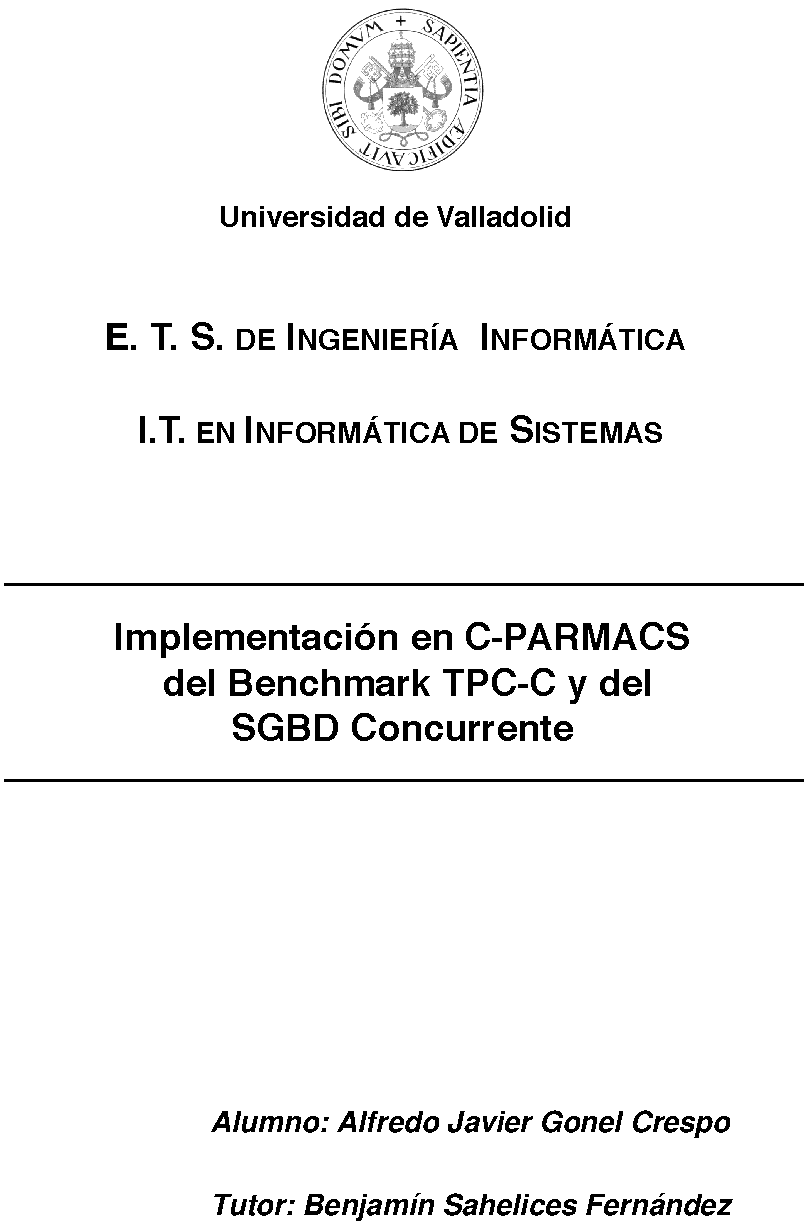
\includegraphics[width=\textwidth,height=\textheight]{portada/portada-orig.pdf}
\end{center}
\end{figure}
\clearpage
% P�gina en blanco
\thispagestyle{empty}
\clearpage

% Para los capitulos
\fancypagestyle{plain}{% 
\fancyhf{} % clear all header and footer fields 
\fancyfoot[RO,LE]{\bfseries \thepage} % except the center 
\renewcommand{\headrulewidth}{0pt} 
\renewcommand{\footrulewidth}{0.6pt}} 

% Para el resto del documento.
\pagestyle{fancy}
\fancyhf{}
\fancyhead[RO]{\rightmark}
\fancyhead[LE]{\leftmark}
\fancyfoot[RO,LE]{\bfseries \thepage}
\renewcommand{\chaptermark}[1]{\markboth{\textbf{\thechapter. #1}}{}} % Formato para el cap�tulo: N. Nombre
\renewcommand{\sectionmark}[1]{\markright{\textbf{\thesection. #1}}} % Formato para la secci�n: N.M. Nombre
\renewcommand{\headrulewidth}{0.6pt} % Ancho de la l�nea horizontal bajo el encabezado
\renewcommand{\footrulewidth}{0.6pt} % Ancho de la l�nea horizontal sobre el pie (que en este ejemplo est� vac�o)
\setlength{\headheight}{1.5\headheight} % Aumenta la altura del encabezado en una vez y media

%Contenidos
\tableofcontents % Tabla de contenido 
\newpage 
\listoffigures % �ndice de figuras 
\newpage 
\listoftables % �ndice de tablas 
\newpage

\chapter{Introducci�n}
Dentro del Departamento de Inform�tica, en el grupo de investigaci�n de
Arquitectura y Tecnolog�a de Computadores (conocido como ATC), se realizan
simulaciones de aplicaciones paralelas (como las que se se pueden encontrar en
Splash-2 \cite{woo95splash}) con el simulador RSIM \cite{pai97rsim}, para 
probar sus trabajos de
protocolos de coherencia cach� \cite{Sahelices00a,Sahelices00b,Llanos00}. Esta
investigaci�n a su vez est� integrada dentro del proyecto {\em Computaci�n de 
Altas Prestaciones IV. Jerarqu�a de Memoria de Altas Prestaciones} de la 
Universidad de Zaragoza (Ref. TIN2004-00739-C02-02). En base a esto y para
mejorar la fiabilidad de los resultados obtenidos se hace necesario ampliar y 
completar el repertorio de aplicaciones y n�cleos disponibles en las simulaciones.

El prop�sito de este proyecto de fin de carrera es m�ltiple:
\begin{itemize}
\item Primero, colaborar con la aplicaci�n que se ha implementado a lo largo del
desarrollo del proyecto, y as� aumentar la gama de aplicaciones disponibles para
las simulaciones del grupo ATC.
\item A la vez que se hace disponible al resto de la comunidad inform�tica un
programa capaz de cuantificar el rendimiento de un sistema paralelo, basado en
un est�ndar y que funciona independientemente de otros sistemas software.
\item Por �ltimo, completar la formaci�n acad�mica de la carrera de Ingenier�a
T�cnica de Inform�tica de Sistemas dando una aplicaci�n a un gran n�mero de
conceptos adquiridos durante la misma.
\end{itemize}

La aplicaci�n que aqu� se detalla es un software de medida de rendimiento,
com�nmente conocido por su nombre en ingl�s \textit{benchmark}. Este benchmark
pretende ser una aplicaci�n ejecutable en entornos UNIX y similares, en los que es
muy com�n encontrarse m�quinas con m�ltiples procesadores. La poder ejecutar la
aplicaci�n en estos entornos UNIX, se ha aplicado la compatibilidad a trav�s del
c�digo fuente, utilizando:
\begin{itemize}
\item El lenguaje de programaci�n C, muy extendido en entornos UNIX, permite
obtener la aplicaci�n ejecutable en dichos entornos UNIX sin cambiar el c�digo
gracias a las especificaciones ANSI-C y POSIX \cite{posix}.
\item La biblioteca de macros PARMACS \cite{parmacs}, para una programaci�n
paralela transportable entre sistemas paralelos con diferente arquitectura de
memoria.
\end{itemize}

\subsubsection{TPC-C}
Este benchmark est� basado en las especificaciones del TPC (\textit{Transaction
Processing Performance Council}) \cite{tpc} conocidas como TPC-C; adem�s 
est� destinado a medir el rendimiento del procesamiento de transacciones en
l�nea simulando diferentes tipos de transacciones y una compleja base de datos
en un entorno empresarial com�n y gen�rico pero que se aproxima bien al uso
actual de los sistemas de bases de datos existentes hoy en d�a.

En la industria de sistemas servidores dicho benchmark es un punto de
referencia;
si bien TPC-C son s�lo unas especificaciones, que aplicadas correctamente dan lugar
a un sistema de medida del rendimiento con unidades comparables entre distintos
sistemas. En el caso del TPC-C, la unidad de medida es la transacci�n, y la
capacidad de los sistemas se compara en transacciones por minuto (tpmC). En
cuanto a los sistemas paralelos, dada la clasificaci�n de las transacciones en 5
tipos, en base a unas reglas de unicidad (ACID), y gracias a la concurrencia de
peticiones , el benchmark TPC-C se convierte en un buen candidato para medir el 
rendimiento de estos sistemas paralelos.

Las especificaciones TPC-C dan lugar a un benchmark, que normalmente es
implementado por empresas propietarias ya sea para medir el rendimiento de los
sistemas que ponen a la venta o para venderlo a las empresas que lo necesiten.
Esto implica que hay muy pocas implementaciones de uso libre y/o con c�digo
abierto para poder investigar, por lo que es interesante ampliar el repertorio
tanto con un dise�o como con una implementaci�n libre.

\subsubsection{Notas del dise�o}
Uno de los objetivos es proporcionar al grupo ATC un sistema m�s para sus
simulaciones usando RSIM.  Uno de los principales problemas de RSIM es el
reducido n�mero de bibliotecas que soporta, luego simular programas complejos
que utilizan un gran n�mero de funciones externas resulta algo inviable, y se
hace necesario que los programas no dependan m�s que de la biblioteca est�ndar de
funciones.

Aunque el dise�o s�lo se ha orientado a PARMACS, si se quiere tener la
posibilidad de trasladar la aplicaci�n de manera sencilla a RSIM, hay que tener
en cuenta que aplicarlo en el dise�o implica que:
\begin{itemize}
\item Hay que analizar m�s all� de las especificaciones, buscando todos los
subsistemas necesarios para la implementaci�n, ya que no podemos depender de
bibliotecas externas.
\item Hay que buscar una arquitectura que abarque todos los subsistemas:
analizar y dise�ar el sistema desde 0.
\item Dado que hemos hablado de una \textit{compleja base de datos} habr� que
dise�arla directamente y no sobre un sistema gestor de bases de datos ya
existente.
\end{itemize}

\subsubsection{Aspectos de la implementaci�n}
Las implicaciones que supone el dise�o de una aplicaci�n desde cero, adem�s del
dise�o de un sistema de almacenamiento, se reflejan fielmente en la
implementaci�n. En cuanto al sistema de almacenamiento, supone la tarea de
codificar un gestor de bases de datos, que aun partiendo de un buen dise�o, es
una traba a superar.

Al estar toda la aplicaci�n implementada en C y usando bibliotecas
est�ndar, este proyecto se convierte en un buen candidato tanto para ser
adaptado a RSIM y poderlo utilizar en las simulaciones;
como para la medici�n de rendimiento, de manera
independiente, de sistemas mono y multiprocesador.

No hay que olvidar que el lenguaje C, sin ser un lenguaje de tan bajo nivel como el
ensamblador, no implementa ni facilita ciertos paradigmas de la programaci�n que
en este caso podr�an ser de mucha ayuda: orientaci�n a objetos, manejo autom�tico de
memoria, etc. Por lo que es necesario una implementaci�n cuidadosa e
ingeniosa en algunos momentos para resolver estos problemas. Aunque de la misma
manera que hace falta dise�ar soluciones ingeniosas, existe el problema de
encontrar fallos en momentos finales del desarrollo.

\subsubsection{Requerimientos}
Por �ltimo, comentar algunos de los conocimientos m�s importantes que han hecho
falta para solucionar todos los problemas encontrados.
\begin{itemize}
\item Ingenier�a del software: necesaria para analizar los requisitos del
est�ndar TPC-C y poder dise�ar una arquitectura sostenible para el sistema. Se
ha hecho un esfuerzo especial en dejar claros los requisitos iniciales y en formar
el dise�o arquitect�nico que define los subsistemas.
\item Programaci�n estructurada: para dar forma a las necesidades del dise�o.
Dado que no se va a utilizar un lenguaje orientado a objetos, hace falta dar
forma a las necesidades del an�lisis mediante las estructuras disponibles en la
programaci�n estructurada.
\item Lenguaje de programaci�n C: usado para reflejar el dise�o en un programa
compilable y ejecutable. Se ha usado este lenguaje sobre todo por la necesidad de utilizarlo m�s tarde en
RSIM, pero tambi�n por la compatibilidad entre sistemas.
\item Estructuras de datos: concretamente �rboles de b�squeda y derivados de
dichos �rboles que sean utilizados actualmente en sistemas gestores de bases de
datos reales.
\item Sistemas operativos y programaci�n paralela: se aplican a la hora de
implementar un sistema de almacenamiento concurrente, que servir� de base s�lida
para el funcionamiento paralelo de la aplicaci�n.
\end{itemize}


\chapter{Fundamentos}
\section{An�lisis de rendimiento}
Las especificaciones del est�ndar TPC-C no son m�s que las especificaciones de
un an�lisis de rendimiento que incluyen la realizaci�n de una herramienta de
medida de rendimiento, pero tambi�n la preparaci�n de una documentaci�n adecuada
as� como una elecci�n de par�metros y factores que analizar. Para entender mejor
qu� es y qu� influye en un an�lisis de rendimiento se va a detallar en qu�
consiste y qu� factores influyen de una manera general.

\subsection{Objetivos del an�lisis de rendimiento}

Los objetivos de cualquier an�lisis de rendimiento de un sistema inform�tico o
de uno de sus componentes dependen del la situaci�n concreta y de la capacidad,
habilidad e intereses de la persona encargada de realizar ese an�lisis (el
analista). Aun con estas dependencias se pueden se�alar varios objetivos
\cite{cambridge00} que
suelen buscar en los an�lisis de rendimiento los cuales son �tiles tanto para
dise�adores de sistemas inform�ticos como para el usuario final.

\begin{itemize}
\item\textbf{Comparar alternativas.} Cuando se necesita adquirir un nuevo
sistema inform�tico, uno se enfrenta a diferentes sistemas con diferentes
caracter�sticas entre los que elegir. Cada caracter�stica de un solo sistema
puede afectar al rendimiento y al precio: memoria, n�mero de procesadores,
interfaz de red, n�mero de discos, sistema operativo, etc. El objetivo de un
an�lisis de rendimiento en este caso es proporcionar informaci�n cuantitativa
sobre qu� configuraci�n es la m�s adecuada bajo unas determinadas condiciones.

\item\textbf{Determinar el impacto de una caracter�stica concreta.} Cuando se
dise�a un nuevo sistema, o cuando se actualiza uno ya existente, se suele
necesitar determinar el impacto causado al a�adir o eliminar una caracter�stica
concreta; por ejemplo, el dise�ador de un nuevo procesador puede querer
determinar cuando es �til a�adir una unidad de punto flotante a la arquitectura,
o si el tama�o de la cach� incluida en el chip es el adecuado. Este es el
an�lisis llamado \textit{comparaci�n antes y despu�s}, ya que se cambia un
componente bien definido del sistema.

\item\textbf{Ajustar el sistema.} El objetivo de un an�lisis de rendimiento
cuando se quieren optimizar los ajustes de un sistema, es encontrar el conjunto
de par�metros con sus valores que producen en su totalidad el mejor rendimiento. En
los sistemas operativos de tiempo compartido, por ejemplo, es posible controlar
el n�mero de procesos que pueden compartir el procesador; el impacto sobre el
rendimiento que perciben los usuarios del sistema puede verse muy afectado por
este n�mero y tambi�n por la cantidad de tiempo asignado a cada proceso. Muchos
otros par�metros del sistema como los tama�os de los almacenes intermedios de
red y disco pueden tambi�n alterar el rendimiento de un sistema, ya que los
impactos en el rendimiento de estos par�metros pueden estar interconectados; el
hecho de encontrar el mejor conjunto de par�metros con sus valores adecuados
puede ser una tarea dif�cil.

\item\textbf{Identificar el rendimiento relativo.} El rendimiento de un sistema
inform�tico s�lo suele tener un significado concreto dentro del contexto de su
rendimiento relativo a alguna otra \textit{cosa}, como otro sistema u otra
configuraci�n del sistema; por eso el objetivo en esta situaci�n puede ser
cuantificar el cambio en el rendimiento relativo a las antiguas
versiones/generaciones del sistema. Otro objetivo puede ser cuantificar
el rendimiento relativo a las necesidades de un cliente o el de los sistemas de la
competencia.

\item\textbf{B�squeda de fallos en el rendimiento.} Buscar fallos en un programa
para que su funcionamiento sea lo m�s correcto posible es lo b�sico en cualquier
aplicaci�n, sin embargo, el an�lisis de rendimiento se convierte en un problema
de b�squeda tambi�n, aunque en este caso de rendimiento. Un programa funciona
correctamente pero lo hace m�s lentamente de lo deseado, por lo que el analista
en este punto busca identificar las causas por las que el programa no cumple con
los requisitos de rendimiento que se esperan de �l; una vez los problemas de
rendimiento se identifican, puede que exista alguna posibilidad de resolverlos. 

\item\textbf{Establecer unas expectativas.} Los usuarios de un sistema
inform�tico pueden hacerse una idea de la capacidad de, por ejemplo, la nueva
generaci�n de sistemas inform�ticos, gracias a que se ha realizado un an�lisis
de rendimiento indicando lo que dichos sistemas son capaces de hacer.

\end{itemize}

En todas estas situaciones, el esfuerzo involucrado en el trabajo de un an�lisis
de rendimiento debe ser proporcional al coste de escoger la decisi�n equivocada;
por ejemplo, si se est�n comparando diferentes fabricantes de sistemas
inform�ticos para conocer cual de ellos es mejor en una decisi�n de compra de
muchos equipos, el coste monetario de escoger la empresa equivocada puede ser
importante, tanto el coste del sistema en si como las �reas de la empresa que se
vean afectadas por esa mala decisi�n. Se ve claramente que en este caso el
an�lisis tiene que ser muy detallado. Aunque por ejemplo, si se est� buscando el
mejor PC para un uso personal, el coste de escoger la opci�n equivocada es
m�nimo, y el an�lisis de rendimiento puede limitarse a leer unos pocos art�culos
de una revista.

\subsection{T�cnicas generales}
Cuando uno se enfrenta a un problema de an�lisis de rendimiento, hay tres
t�cnicas fundamentales que se pueden usar para encontrar la soluci�n adecuada.
Estas son: \textit{medidas} de los sistemas actuales, \textit{simulaci�n} y
\textit{modelado anal�tico}. Las medidas de los sistemas existentes normalmente proporcionan los mejores
resultados ya que teniendo las herramientas de medida adecuadas, no hace falta
hacer ninguna simplificaci�n, s�lo queda utilizarlas; lo que hace que los
resultados basados en las medidas de un sistema existente sean m�s cre�bles
cuando se presentan a otras personas. Aun as� las medidas de estos sistemas no
suelen ser flexibles y s�lo proporcionan informaci�n del sistema analizado. Un
objetivo com�n del an�lisis de rendimiento es caracterizar c�mo el rendimiento
de un sistema cambia al variar ciertos par�metros; en un sistema existente
puede ser dif�cil, si no imposible, cambiar alguno de estos par�metros, por lo que
evaluar el impacto en el rendimiento de dicho par�metros es tambi�n imposible.
Medir ciertos aspectos del rendimiento en un sistema actual puede suponer una
tarea costosa en tiempo y dif�cil, as� que aunque las medidas de sistemas
reales nos ofrezcan datos muy fiables, las dificultades y limitaciones
existentes hacen que sean necesarias otras t�cnicas para buscar soluciones.


La simulaci�n de un sistema inform�tico es un programa escrito para modelar
caracter�sticas importantes del sistema que est� siendo analizado; ya que el
simulador no es nada m�s que un programa, puede modificarse f�cilmente para
estudiar el impacto de cambios en casi cualquiera de los componentes que se
simulan. El coste de una simulaci�n incluye el tiempo requerido para escribir y
depurar el programa de simulaci�n as� como el tiempo de cada simulaci�n;
dependiendo de la complejidad del sistema que se esta simulando, y el nivel de
detalle del modelo, estos costes pueden ser relativamente bajos o moderados
comparados con el coste de comprar una m�quina real en la cual realizar los
experimentos.

La principal limitaci�n de un an�lisis de rendimiento basado en simulaciones es
que es imposible modelar hasta el m�s m�nimo detalle del sistema que se est�
estudiando, por lo que se necesita simplificar algunos conceptos y realizar
algunas asunciones para que sea posible escribir un modelo que se pueda
ejecutar en un tiempo razonable. Estas simplificaciones pueden limitar la
exactitud de los resultados y por lo tanto reducir la confianza que se puede
tener en el modelo comparado con un sistema real, sin embargo, la simulaci�n
disfruta de una gran popularidad para el an�lisis de sistemas inform�ticos
(V�ase RSIM por ejemplo) dado el alto grado de flexibilidad y su relativa
facilidad de implementaci�n.

La tercera t�cnica disponible para el analista es el modelado anal�tico; el
modelo anal�tico es una descripci�n matem�tica del sistema, que comparada con
una simulaci�n o unas medidas de un sistema real, obtiene unos resultados menos
cre�bles y menos precisos. No obstante, un modelo anal�tico simple puede
proveernos r�pidamente de peque�os detalles dentro del conjunto general del
sistema o de alguno de sus componentes; estos peque�os detalles internos pueden
ser usados para ayudar a centrar unas medidas m�s detalladas o un modelo de
simulaci�n m�s concreto. Un modelo anal�tico puede ayudar a discernir si los
resultados producidos por un simulador o los valores obtenidos de un sistema
real son razonables o no.

\subsubsection{Un ejemplo}

El retraso que se observa en una aplicaci�n cuando accede a memoria puede tener
un gran impacto sobre el tiempo de ejecuci�n total; medidas directas de dicho
retraso en una m�quina existente pueden ser dif�ciles de obtener, aunque dado
que los pasos que se ejecutan para acceder a una sistema de memoria complejo no
est�n accesibles normalmente desde una aplicaci�n de usuario, un programador
avanzado puede ser capaz de escribir un simple programa que ejecute porciones
espec�ficas de c�digo en dicha arquitectura de memoria para poder obtener algunos
par�metros importantes del sistema. Por ejemplo, el tiempo de ejecuci�n de un
programa sencillo que referencia una y otra vez la misma variable puede usarse
para estimar el tiempo que se necesita para acceder al primer nivel de cach�; de
la misma manera, un programa que siempre fuerza fallos en la cach� puede servir
para medir indirectamente el tiempo de acceso a  la memoria principal.
Desafortunadamente, el impacto de esos par�metros del sistema en el tiempo de
ejecuci�n de una aplicaci�n completa es muy dependiente de las referencias a
memoria que realice dicha aplicaci�n, y obtener un patr�n de esas referencias
puede ser dif�cil.


Por otro lado, la simulaci�n es una potente t�cnica para estudiar el
comportamiento de los sistemas de memoria, dado su alto grado de flexibilidad,
cualquier par�metro de la memoria incluida la granularidad de la cach�, los
tiempos de acceso relativos, los tama�os de la cach� y la memoria, etc, puede
ser f�cilmente alterado para estudiar su impacto en el rendimiento. Puede ser
todo un reto modelar completamente el solapamiento de los retrasos de memoria, y
la ejecuci�n de otras instrucciones en procesadores que tiene sistemas como la
ejecuci�n fuera de orden, predicci�n de saltos, acceso a cach� no bloqueantes,
etc. Aun con las simplificaciones y asunciones, los resultados de una
simulaci�n detallada proporcionan detalles internos �tiles del efecto de la
memoria en el rendimiento de un programa concreto.

Por �ltimo, se puede desarrollar un modelo anal�tico simple: Sea $t_c$ el retardo
observado al acceder a una direcci�n de memoria si la memoria a la que accedemos
se encuentra en la cach�, sea $t_m$ el retardo al acceder a la memoria principal,
sea h el ratio de aciertos de la cach� (la cantidad de accesos a memoria que son
resueltos por la cach� sin acceder a la memoria principal), por lo que el ratio
 de fallos en la memoria ser� $h - 1$. Podemos concluir que el tiempo medio
 necesario para un acierto en la cach� es $h * t_c$, mientras que el tiempo medio
 para los fallos es $t_m * (h - 1)$. El modelo simple del tiempo medio de acceso
 a memoria es:
\begin{equation}
t_avg = h*t_c + (1 - h)*t_m
\label{modelosimple}
\end{equation}

Para aplicar este modelo simple a un programa espec�fico se necesita conocer el
ratio de aciertos (h) para ese programa; as� como los valores de $t_c$ y $t_m$
para el sistema, que se pueden encontrar en las especificaciones del fabricante
o pueden ser obtenidos mediante medidas como se describi� anteriormente; por
�ltimo el ratio de aciertos para un programa normalmente es m�s dif�cil de
obtener. En definitiva, un modelo simple puede aportar informaci�n sobre los
efectos de incrementar ciertos par�metros en el sistema.

\subsubsection{Resumen}

Vamos a ver un resumen de estas 3 t�cnicas as� como de los par�metros que las
diferencian (\tablename\ \ref{tab:resumentecnicas}).

\begin{table}[htb]
\begin{center}
\begin{tabularx}{\linewidth}{XXXX}
\hline
\textbf{Caracter�stica} & \textbf{Modelo anal�tico} & 
\textbf{Simulaci�n}     & \textbf{Medidas reales} \\
\hline
Flexibilidad & Alta & Alta  & Baja \\
Coste        & Bajo & Medio & Alto\\
Credibilidad & Baja & Media & Alta\\
Exactitud    & Baja & Media & Alta\\
\hline
\end{tabularx}
\end{center}
\caption{Tabla resumen de las t�cnicas de an�lisis}\label{tab:resumentecnicas}
\end{table}

La \textit{flexibilidad} de una t�cnica indica c�mo de f�cil es cambiar la
configuraci�n del sistema que se est� estudiando; el \textit{coste} corresponde
al tiempo y dinero necesario para realizar el experimento adecuado dependiendo
de la t�cnica; la \textit{credibilidad} de una t�cnica es alta si los resultados
producidos usando esa t�cnica son lo m�s reales que se pueda. Es m�s f�cil para
alguien creer que el tiempo de ejecuci�n de una aplicaci�n estar� dentro de un
rango que uno puede demostrar en una m�quina actual que el rango obtenido de una
simulaci�n; por la misma regla, son m�s reales los resultados obtenidos de una
simulaci�n que de un modelo anal�tico. Por �ltimo, la \textit{exactitud} de una
t�cnica indica c�mo de cercanos son los resultados a los de un sistema real.

La elecci�n de una soluci�n espec�fica depende del problema que se quiera
resolver; por lo que una de las  habilidades que debe desarrollar un analista
del rendimiento de sistemas inform�ticos, es la de determinar la t�cnica m�s
apropiada dada una situaci�n concreta.

\subsection{Errores comunes en los an�lisis de rendimiento}
Para favorecer el uso de la metodolog�a adecuada para evaluar el rendimiento,
en esta secci�n se van a exponer una serie de errores que en los que se incurre de manera
habitual en muchos proyectos de evaluaci�n de rendimiento. La mayor�a de errores
listados no se cometen de manera intencionada, sino que ocurren por errores de
concepci�n, suposiciones o falta de conocimiento de las t�cnicas de medida de
rendimiento.

\begin{enumerate}
\item \textbf{No tener objetivos.} Tener alguna meta es la parte m�s importante
de cualquier esfuerzo, y sin ella dicho esfuerzo esta avocado al fracaso; en
este aspecto los proyectos de medida de rendimiento no son ninguna excepci�n.
La necesidad de una meta puede sonar
obvio pero muchos proyectos comienzan sin ning�n objetivo definido; por ejemplo,
una persona dedicada a analizar el rendimiento que es contratada e insertada en
el equipo de dise�o, puede empezar a modelar un dise�o, pero cuando
se le pregunta por los objetivos el analista suele contestar que el modelo es el
que ayudar� a resolver las preguntas que puedan surgir. Es muy com�n o�r que los
modelos son lo suficientemente flexibles para ser adaptados a diferentes
problemas, pero la realidad es que se hacen necesarios modelos concreto con
objetivos concretos; las medidas utilizadas y la carga de trabajo empleada
dependen al final del objetivo. Qu� parte del sistema necesite ser estudiada
var�a dependiendo del problema, por ello antes de escribir la primera l�nea de
c�digo o formula de un modelo, o antes de establecer un experimento que haga una
medici�n, es importante que el analista entienda el sistema e identifique el
problema que necesita ser resuelto, lo que ayudar� a elegir correctamente: la
m�trica, la carga de trabajo y la metodolog�a en general.Establecer unos
objetivos no es un trabajo sencillo, ya que los problemas que se presentan en
las medidas de rendimiento suelen ser vagos y abstractos.

\item\textbf{Objetivos parciales.} Otro error com�n es declarar de manera impl�cita o
explicita cierto \textit{partidismo} a la hora de indicar los objetivos
iniciales. Por ejemplo, si nuestro objetivo es ``Mostrar que nuestro sistema es
mejor que los dem�s'', el problema se convierte en la b�squeda de medidas y
cargas de tal manera que nuestro sistema salga siempre vencedor, en vez de
buscar las medidas y cargas de trabajo que comparan realmente los dos sistemas.
Por ello una regla muy importante es ser imparcial y no tener ideas
preconcebidas para obtener unas conclusiones independientes y no guiadas por
ciertas creencias iniciales.

\item\textbf{Mala aproximaci�n al problema.} Normalmente un analista adopta una
aproximaci�n mala cuando no tiene ning�n sistema o metodolog�a para entender el
problema; escoger par�metros, factores, medidas y cargas de trabajo de manea
aleatoria, lo que lleva a conclusiones imprecisas. Hace falta un m�todo para
comprender el problema paso por paso, para identificar los objetivos,
par�metros, factores, medidas y cargas de trabajo de manera adecuada.

\item\textbf{No entender el problema.} Un analista con poca experiencia siente que no
se ha hecho nada hasta que se ha construido un modelo y se tienen algunos
resultados num�ricos; pero con el tiempo uno se da cuenta de que gran parte del
esfuerzo del an�lisis se invierte en definir correctamente el problema, pudiendo
consumir hasta un 40\% del tiempo \cite{theart91}. Como dice el refr�n \textit{un
problema bien explicado ya tiene la mitad resuelto}, del resto, una gran parte
del tiempo se invierte en alternativas de dise�o, interpretaci�n de resultados y
presentaci�n de conclusiones; el desarrollo del modelo en si es una peque�a
parte del proceso. As� como un coche o un tren es un medio para llegar a un
lugar concreto, y no un fin en si mismos, los modelos son los medios para
alcanzar las conclusiones, no son el resultado final. Un analista experto en el
modelado de medidas de rendimiento pero que no se esfuerza en entender el
problema concreto, encuentra que sus modelos son ignorados por aquellas personas
que necesitan unos datos para tomar decisiones, ya que ellos necesitan una ayuda
en sus decisiones, no un modelo.

\item\textbf{M�trica de rendimiento mal elegida.} Una m�trica se refiere al criterio
usado para cuantificar el rendimiento del sistema, por ejemplo las m�tricas m�s
utilizadas son la capacidad de procesar datos (throughput) y el tiempo de
respuesta. La elecci�n de las m�tricas adecuadas depende de los servicios que
sistema vaya a proveer; por ejemplo el rendimiento de una CPU se compara
bas�ndose en su capacidad de procesar datos, lo que se suele medir en t�rminos
de millones de instrucciones por segundo (MIPS); aun as�, comparar los MIPS de
dos CPU de diferente arquitectura como RISC (Reduced Instruction Set Computers)
y CISC (Complex Instruction Set Computers), no tiene mucho sentido ya que las
instrucciones de cada CPU son totalmente distintas. El error usual es utilizar
m�tricas f�cilmente calculables en vez de m�tricas relevantes que son m�s
dif�ciles de calcular.

\item\textbf{Carga de trabajo no representativa}. La carga de trabajo usada para
comparar dos sistemas debe ser representativa del uso actual y real del
sistema; por ejemplo, si los paquetes en una red son una mezcla de dos tama�os:
cortos y largos, la carga de trabajo para comparar dos redes debe consistir
tanto en paquetes cortos como largos.
La elecci�n de la carga de trabajo tiene un impacto significativo en los
resultados del estudio de rendimiento, ya que la carga equivocada puede dar
conclusiones err�neas.

\item\textbf{T�cnica de evaluaci�n equivocada}. Hay tres t�cnicas de evaluaci�n:
medir, simular y modelar anal�ticamente. Los analistas normalmente tienen
preferencia por una de estas tres t�cnicas, y la utilizan constantemente;
aplicando otro refr�n \textit{Cuando aprendes a manejar un martillo todos los
problemas son clavos}, pero el basarse en una sola t�cnica produce un modelo
que aunque sea el que mejor se sabe resolver no tiene que ser el que mejor
resuelva el problema, introduciendo fen�menos que no est�n en el sistema real y
dejando fuera par�metros que pueden ser importantes.

  
\item\textbf{Pasar por alto par�metros importantes.}  
Es una buena idea hacer una lista lo m�s completa posible de componentes del
sistema y de la carga de trabajo que afecta a su rendimiento, estas
caracter�sticas son los denominados par�metros; por ejemplo, para un sistema
operativo los par�metros pueden ser: la cantidad de tiempo que un proceso esta
en la CPU, o el tama�o de memoria ocupado por el trabajo actual. Estos
par�metros de carga pueden incluir el n�mero de usuarios, patrones de llegada de
peticiones, prioridad, etc; es trabajo del analista escoger un grupo de valores
para cada uno de esos par�metros; ya que los resultados finales del estudio
dependen de esa elecci�n, el hecho de pasar por alto un solo par�metro
importante puede hacer que los resultados no tengan ninguna validez.

\item\textbf{Pasar por alto factores importantes.} Cuando un par�metro var�a en
el estudio, se le llama factor; por ejemplo, de los par�metros del punto
anterior, el n�mero de usuarios puede ser un factor y el resto de par�metros
permanecer fijos. No todos los par�metros tienen el mismo efecto en el
rendimiento, por lo que es importante identificar aquellos par�metros que si
var�an afectan de manera importante al rendimiento del sistema, y usar esos
par�metros como factores. Un ejemplo, si la tasa de llegada de paquetes en
una red afecta m�s al tiempo de respuesta que el tama�o de los paquetes, ser�
mejor utilizar varias tasas de llegada de paquetes en el estudio que varios
tama�os de paquetes.

A la hora de elegir un factor entre los par�metros, aquellos factores que est�n
bajo el control del usuario o la persona que toma las decisiones y que pueden
ser f�cilmente cambiados, son los mejores factores posibles ya que no merece la
pena malgastar tiempo comparando alternativas que el usuario final no puede
adoptar debido a que no puede cambiarlas de ninguna manera. Tambi�n es importante
entender las caracter�sticas aleatorias de algunos componentes del sistema que
pueden afectar en el rendimiento, y muy probable que algunos de esos par�metros
sean desconocidos para el analista (por ejemplo el funcionamiento del
programador de acceso a disco del sistema), por lo que aunque puedan tener
importancia, el analista los desechar� por no conocerlos. La elecci�n de
factores debe basarse en su importancia no en el conocimiento que se tenga sobre
ellos.

\item\textbf{Dise�o del experimento mal realizado.} Este dise�o est�
relacionado con el n�mero de medidas o de simulaciones que se van a realizar y
los valores de los par�metros en cada experimento. La elecci�n correcta de estos
valores ayuda a sacar m�s informaci�n de cada experimento, de esta manera no se
desperdicia el tiempo ni los recursos utilizados. Por ejemplo:
dise�ando los experimentos de manera ingenua, en cada experimento se altera cada
factor de uno en uno, lo que puede llevar a equivocaciones si dos par�metros son
dependientes y no se cambian a la vez.
\item\textbf{Nivel de detalle inadecuado.} El nivel de detalle usado a la hora
de modelar un sistema tiene un gran impacto en la formulaci�n del problema,
debido al exceso de datos o a la falta de datos. Para comparar alternativas que
simplemente son peque�as variaciones de un mismo modelo es mejor indicar esas
variaciones que hacer un modelo de m�s alto nivel. Por otro lado, cuando se
comparan alternativas muy diferentes, es bueno usar un modelo de alto nivel que
permita comparar alternativas muy diferentes de manera r�pida. El error que se
suele cometer es detallar demasiado cuando se necesita un modelo de alto nivel,
y abstraerse cuando se necesita un modelo de bajo nivel.

\item\textbf{Ignorar el an�lisis de los resultados.} Uno de los mayores
problemas con las medidas en los proyectos de medida de rendimiento, es que los
analistas que los realizan son buenos con las t�cnicas de medici�n pero no
tienen base, conocimientos y/o experiencia analizando los datos. Recogen gran
cantidad de datos pero no saben qu�  analizar o c�mo interpretarlos, de tal
manera que no se obtiene un resumen de los datos y solo se entregan los datos en
bruto. Por lo que se hace necesario tener un equipo que conozca c�mo analizar
esos datos.

\item\textbf{An�lisis equivocado.} Hay un buen n�mero de errores comunes a la
hora de realizar medidas, simulaciones y modelos anal�ticos, como por ejemplo
simulaciones cortas, medias demasiado alteradas, etc.

\item\textbf{An�lisis insensible.} Es habitual que los analistas pongan
demasiado �nfasis en los resultados de sus an�lisis, present�ndolos como hechos
m�s que como evidencias. El hecho es que los resultados pueden ser sensibles a
la carga de trabajo y a par�metros del sistema, y esto se suele obviar; por lo
que sin un an�lisis sensible a estos par�metros uno no puede estar seguro si las
conclusiones cambiar�an si el an�lisis se realiza con una configuraci�n
ligeramente diferente, adem�s sin un an�lisis sensible a los par�metros, es
dif�cil acceder a la importancia relativa de los diferentes par�metros.
 
\item\textbf{Ignorar los errores en la entrada.} Los par�metros de inter�s
algunas veces no pueden ser medidos directamente, por lo que se toman medidas de
otra variable y se usa para estimar el par�metro deseado; por ejemplo, en una red
de ordenadores donde los paquetes son almacenados en una lista enlazada de almacenes
temporales (buffers), y cada almac�n tiene un tama�o determinado, dado el n�mero
de almacenes requerido para almacenar los paquetes es imposible predecir el
n�mero de paquetes o lo que ocupa exactamente cada paquete. Estas situaciones
introducen cierto desconocimiento de los datos de entrada, y el analista
necesita ajustar el nivel de confianza de los datos de salida de ese modelo ya
que los datos de entrada no son muy fiables. 

\item\textbf{Valores extremos.} Tambi�n hay que tener cuidado con valores extremos, 
los llamados outliers, a la
hora de realizar la estad�stica correspondiente, ya que pueden afectar mucho a
los resultados; pero para poder descubrir esos valores extremos, y sobre todo
cuales se pueden ignorar y cuales no, hace falta un
conocimiento profundo y cuidadoso del sistema que esta siendo analizado.

\item\textbf{Asumir un futuro sin cambios.} Normalmente se asume que el futuro
ser� el mismo que el pasado, por lo que se usa un modelo basado en la carga y
rendimiento observado en el pasado para predecir el rendimiento en el futuro. Se
asume que en el futuro la carga y el rendimiento del sistema ser� el mismo, pero
dependiendo de la cantidad de tiempo y de que se quiera asumir, esto puede no
ser verdad.

\item\textbf{Ignorar la variabilidad.} Analizar s�lo la media de rendimiento y
no analizar la variabilidad es lo m�s sencillo, pero no es imposible analizarla.
Si la variaci�n es alta, la media por si sola no ayuda en nada a la hora de
tomar decisiones; por ejemplo, el uso diario de ancho de banda puede no
significar nada, pero el uso por horas puede aportar informaci�n �til.

\item\textbf{An�lisis demasiado complejo} Si dos an�lisis dan la misma
conclusi�n, es preferible utilizar aquel an�lisis que es m�s simple y f�cil de
explicar. Metas demasiado ambiciosas y modelos demasiado complejos dan lugar a
an�lisis dif�cilmente entendibles; es mejor empezar con modelos o experimentos
simples, e ir introduciendo complicaciones poco a poco hasta llegar a un nivel
de detalle aceptable.

Hay que tener cuidado a veces con los modelos que se realizan en el �mbito
acad�mico; muchas veces en estos c�rculos se tiende a intentar modelar y
resolver problemas complejos, m�s que a intentar dar soluciones a modelos
simples. En el mundo industrial, donde la gente que toma decisiones no tiene
ning�n inter�s por las t�cnicas utilizadas y donde existe hay poco tiempo para
realizar los an�lisis, se necesitan modelos simples y gente capaz de sacar
conclusiones aceptables de esos modelos simples.

\item\textbf{Presentaci�n inadecuada de los resultados.} Una lista que no
produce resultados �tiles es un fallo, y esto normalmente se debe a que el
an�lisis expone unos resultados que no son entendibles por aquellos que los van
a utilizar. Desde dise�adores de un sistema, compradores o patrocinadores de un
proyecto; vender los resultados a los que tomas las decisiones es labor del
analista, por lo que se necesita un especial cuidado a la hora de usar palabras,
im�genes y gr�ficos para explicar los resultados. La medida correcta para el
rendimiento de un sistema no es el n�mero de an�lisis realizado sino aquellos
an�lisis que han servido de algo a las personas que los han utilizado.

\item\textbf{Ignorar aspectos sociales.} Para presentar correctamente los
resultados hacen falta dos habilidades: por una lado saber hablar y escribir y
por otro saber modelar y analizar. Debido a que es importante que los resultados
sean aceptados y entendidos se requiere cierta ingenier�a social para que los
destinatarios puedan creer, entender y aceptar los resultados. Tambi�n existe la
necesidad de comunicaci�n entre miembros del equipo, exponer e intercambiar
resultados, de ah� que una de las habilidades necesarias del analista sea la de
tener facilidad de intercambiar resultados con otras personas. 

\item\textbf{Omitir asunciones y limites.} Todo an�lisis tiene aspectos asumidos
y limitaciones que normalmente no se incluyen en el informe final, lo que puede
llevar al usuario a aplicar el an�lisis en otro contexto donde esas asunciones
no son v�lidas; a veces los analistas listan las asunciones al principio del
informe, pero olvidan las limitaciones al final y hacen conclusiones sobre
entornos en los que el an�lisis no es aplicable.
\end{enumerate}

Esta peque�a discusi�n sobre errores comunes hace posible presentar una lista de
preguntas que se pueden realizar de manera general sobre cualquier an�lisis de
rendimiento; todas estas cuestiones tienen que responderse afirmativamente.  

\begin{enumerate}
\item �Est� el sistema definido correctamente?
\item �Est�n los objetivos definidos de manera imparcial?
\item �Se han seguido sistem�ticamente todos los pasos del an�lisis?
\item �Se entiende el problema correctamente antes de analizarlo?
\item �Son relevantes las medidas de rendimiento en el problema actual?
\item �Es la carga de problema la adecuada para este problema?
\item �Se ha escogido correctamente la t�cnica de evaluaci�n?
\item �Est� completa la lista de par�metros que afectan al sistema?
\item �Est�n todos los par�metros que afectan al rendimiento marcados como
factores que ser�n variados?
\item �El experimento dise�ado es eficiente en t�rminos de tiempo y resultados?
\item �Es el nivel de detalle adecuado?
\item �Los resultados obtenidos est�n presentados con un an�lisis y con una
interpretaci�n?
\item �La estad�stica del an�lisis es correcta?
\item �Es el an�lisis sensible a los par�metros y carga del sistema?
\item �Los errores en la entrada producen solamente peque�os cambios en los
resultados?
\item �Se han identificado y tratado correctamente los valores extremos?
\item �Se han modelado los posibles cambios que pueden ocurrir en un futuro en
el sistema y en el modelo?
\item �Se ha tenido en cuenta que cantidad de variaci�n de la entrada existe?
\item �Se ha tenido en cuenta que cantidad de variaci�n hay en los datos
analizados?
\item �Es el an�lisis f�cil de explicar?
\item �Est� la presentaci�n adaptada a la audiencia?
\item �Se han presentado los resultados de manera gr�fica tanto como se ha
podido?
\end{enumerate}

\section{M�tricas del rendimiento}
\subsection{�Qu� es una m�trica de rendimiento?}

Antes de entender cualquier aspecto del rendimiento de un sistema inform�tico,
hay que concretar exactamente que cosas es �til e interesante medir. Normalmente
las caracter�sticas b�sicas que se miden en un sistema inform�tico son:
\begin{enumerate}
\item La cantidad de veces que ocurre un evento.
\item La duraci�n de un intervalo de tiempo.
\item El valor de un par�metro concreto.
\end{enumerate}

Por ejemplo, puede que necesitemos contabilizar cu�ntas veces un procesador
inicia una petici�n de entrada/salida, cu�nto tiempo dura cada una de esas
peticiones, o cu�ntos bits se transmiten o almacenan en cada petici�n.

Para esos valores que deseamos medir, podemos obtener el valor actual
del par�metro adecuado para describir el rendimiento del sistema. Dicho valor se
llama \textit{m�trica de rendimiento} o unidad de medida del rendimiento.

Si estamos interesados concretamente en el tiempo, cantidad o tama�o del valor
medido, podemos usar el valor directamente como nuestra unidad de medida del
rendimiento del sistema, aunque lo normal es normalizar y relacionar dichos
datos, como por ejemplo: operaciones por segundo. Este tipo de unidad se llama
\textit{unidad de ratio} o \textit{capacidad de proceso}, y se calcula
dividiendo la cantidad de eventos que ocurren en un intervalo de tiempo entre
dicho intervalo de tiempo. Ya que estas medidas est�n normalizadas a una unidad
de tiempo com�n, como pueden ser los segundos, son �tiles para comparar
diferentes mediciones realizadas a lo largo de diferentes intervalos de tiempo.


El escoger una m�trica de rendimiento adecuada depende de los objetivos y del
contexto actual, as� como del coste que se requiere para obtener la informaci�n
necesaria para dicha m�trica. Por ejemplo, suponiendo que se necesita escoger
entre dos sistemas inform�ticos para usar durante un corto periodo de tiempo y
una tarea especifica (como usar un procesador de texto); dado que la
penalizaci�n por hacer una mala elecci�n no es mucha, el escoger la frecuencia
de reloj como m�trica de rendimiento puede ser una buena opci�n; pero desde que
la frecuencia de reloj no es una m�trica aceptable de rendimiento, hay que
escoger una unidad mejor, sobre todo si se necesita comparar una gran cantidad de
esos sistemas inform�ticos. Hay que tomarse un tiempo para escoger una unidad de
medida que sea rigurosa y real, lo que nos lleva a preguntarnos �Cual es una
buena unidad de medida?

\subsection{Caracter�sticas de una buena m�trica de rendimiento}
Se pueden utilizar muchas y muy diferentes unidades de medida de rendimiento
para describir un sistema inform�tico; algunas han sido y son muy utilizadas,
como los MIPS (Millones de instrucciones por segundo) y los MFLOPS (Millones de
operaciones en punto flotante por segundo). Pero el tiempo demuestra que no
todas estas medidas son buenas, en el sentido que pueden llevar a confusi�n y/o
errores; por ello es necesario entender las caracter�sticas de una
\textit{buena} m�trica de rendimiento, lo que nos ayudar� a decidir qu� unidades
de las que est�n disponibles se utilizaran en cada situaci�n particular, o si es
necesario desarrollar una nueva unidad de medida.

Una unidad de medida que satisfaga todos los requisitos \cite{cambridge00} 
que se exponen a continuaci�n, es una unidad de medida �til para un analista, y
le permite realizar comparaciones precisas y detalladas entre diferentes
mediciones. Este criterio fue desarrollado observando los resultados de muchos
an�lisis de rendimiento a lo largo de muchos a�os; no es que sean unos
requerimientos absolutos sino que al no cumplirse pueden inducir a conclusiones
err�neas.
\begin{enumerate}
\item\textbf{Linealidad.} Desde que los humanos tendemos a pensar en t�rminos
lineales, el valor de la unidad de medida debe ser proporcional al rendimiento
de la m�quina; esto quiere decir que si el valor cambia una cierta proporci�n,
el rendimiento del sistema debe variar en dicha proporci�n. Esto es lo m�s obvio
de las medidas, por ejemplo, si un sistema es el doble de r�pido (usando una
unidad de medida de velocidad) que otro, uno
espera que sus tareas se ejecuten en la mitad de tiempo, y si fuera el triple de
r�pido, se esperar�a completar las tareas en un tercio del tiempo original.


No todas las m�tricas son lineales, las m�tricas logar�tmicas como los dB usados
para describir la intensidad, por ejemplo del sonido; esta unidad no es lineal,
y el incremento de una unidad significa el incremento en 10 de la magnitud
observada. Estas medidas no son malas, pero las medidas lineales son m�s
intuitivas a la hora de presentar resultados en los an�lisis de rendimiento.

\item\textbf{Confianza.} Una unidad de medida de rendimiento se considera de
confianza si un sistema A siempre adelanta a otro sistema B cuando los valores
correspondientes en dicha unidad para los dos sistemas indican que A debe
adelantar a B. Pongamos un ejemplo, tenemos una unidad nueva llamada PICS que
mide el rendimiento de programas de procesamiento de texto; medimos un sistema A
y encontramos que los PICS para ese sistema son 128, y el PICS para el sistema B
es 97; la unidad de medida PICS es de confianza si siempre el sistema A es mejor
que el sistema B a la hora de ejecutar programas de procesamiento de texto.

Mientras que esta caracter�stica parezca obvia y no necesaria, muchas veces se
usan unidades de medida que no satisfacen este requerimiento; por ejemplo los
MIPS o la velocidad de reloj, son unidades de medida que no dan confianza. No es
raro encontrar procesadores que aun teniendo una frecuencia de reloj m�s baja,
son mucho m�s potentes que otros que tienen frecuencias de reloj m�s altas.

\item\textbf{Repetibilidad.} Una unidad de medida es repetible si el mismo valor
usando esa unidad es medible cada vez que se ejecuta el mismo experimento, lo
que tambi�n implica que dicha unidad sea determinista.

\item\textbf{Facilidad de medida.} Si una unidad no es f�cil de medir, es
dif�cil que alguien la use; y cuanto m�s dif�cil sea de medir directa o
indirectamente, m�s posibilidades hay de que dicha medida sea tomada de manera
incorrecta; y es peor un valor mal medido (que se contabiliza en los resultados)
que una mala unidad de medida (que no se escoge para contabilizar el
rendimiento).

\item\textbf{Consistencia.} Una unidad de medida consistente es aquella en la que
sus unidades y su definici�n permanecen constantes a lo largo de muchos
sistemas diferentes y configuraciones diferentes del mismo sistema. Si las
unidades no son consistentes, es imposible utilizarlas para comparar el
rendimiento de sistemas distintos o de distintas configuraciones. Unidades como
los MIPS o MFLOPS, no satisfacen ese requerimiento.

\item\textbf{Independencia.} Mucha gente compra sistemas inform�ticos bas�ndose
en la comparaci�n de valores de m�tricas de rendimiento muy comunes, por lo que
no es normal encontrar cierta presi�n en los fabricantes para desarrollar y
optimizar sus sistemas y que dicho valor de esa m�trica mejore sustancialmente.
Para prevenir esta influencia negativa una buena m�trica tiene que ser
resistente a estos trucos.
\end{enumerate}

\subsection{Procesadores y sus unidades de rendimiento}
Una gran variedad de m�tricas de rendimiento han sido propuestas y usadas en el
mundo de la inform�tica; desgraciadamente muchas de esas unidades de medida no
son buenas (como se defini� en la secci�n anterior), o se usan y/o interpretan
de manera incorrecta. Se va a listar una serie de m�tricas muy comunes y se va a
analizar su \textit{bondad} respecto a las caracter�sticas anteriores.

\subsubsection{La frecuencia de reloj}
En muchos anuncios de sistemas inform�ticos, uno de las partes que m�s se
enfatiza es la frecuencia de reloj del procesador central, lo que implica que se
intenta convencer al comprador que un sistema a 250MHz ser� siempre m�s r�pido
que otro a 200MHz. Esta unidad de medida ignora completamente como se realizan
los c�lculos en cada ciclo de reloj, ignora las complejas interacciones del
procesador con el sistema de memoria y la entrada/salida, y sobre todo, ignora
que puede que el procesador sea realmente el cuello de botella del rendimiento
del resto del sistema.

Analizando las caracter�sticas de la frecuencia de reloj en busca de una buena
unidad de rendimiento, encontramos que es una unidad repetible ya que es
constante para un sistema dado, es f�cil de obtener porque aparece en las
especificaciones, es consistente ya que el valor de los MHz se define de la
misma manera en todos los procesadores, y es independiente ya que ninguna
aplicaci�n puede alterar eso. Pero existen varios problemas y es que no es una
unidad lineal y no es una unidad de confianza; ya que como mucha gente puede
demostrar, el tener un procesador con un reloj m�s r�pido no significa que el
ordenador vaya m�s r�pido que otro con velocidad de reloj inferior. En
definitiva, esta unidad no es una buena unidad para medir el rendimiento.

\subsubsection{MIPS}
La cantidad de datos procesados o la proporci�n de datos ejecutados es una
medida basada en dicha cantidad de datos entre una unidad de tiempo; dado que
dicho tiempo suele estar siempre en segundos, estas medidas son �tiles para
comparar velocidades relativas: un coche a $50 m/seg$ va m�s r�pido que uno a
$35 m/seg$.

La unidad de medida MIPS es un intento de desarrollar una medida proporcional
para los sistemas inform�ticos que permita una comparaci�n directa de su
velocidad. Mientras que en el mundo f�sico la velocidad es medida mediante la
distancia recorrida por unidad de tiempo, los MIPS definen la distancia como la
ejecuci�n de una instrucci�n, siendo los MIPS: millones de instrucciones por
segundo, y se definen como:
\begin{equation}
MIPS = \frac{n}{t_e * 10^6}
\end{equation}

De esta manera, los MIPS son f�ciles de calcular (punto 4), repetibles (punto 3)
e independientes (punto 6); desgraciadamente no satisfacen ninguno de los otros
puntos que identifican a una buena medida de rendimiento. No es lineal, ya que
doblando los MIPS no se dobla el rendimiento, y no es de confianza ni
consistente debido a que no se relaciona mucho con el rendimiento.

El problema estriba en que la unidad MIPS en cada procesador significa una
cantidad diferente de proceso realizado, ya que no todos los procesadores
realizan el mismo trabajo con una instrucci�n. Por ejemplo, un procesador puede
tener una instrucci�n de salto que compruebe un bit de condici�n, y otro en esa
misma instrucci�n adem�s decremente un contador; en este ejemplo se ve
claramente como el segundo procesador realiza m�s trabajo en una misma
instrucci�n. Las diferencias entre la cantidad de proceso de cada instrucci�n
son las diferencias entre los procesadores RISC y CISC, que hacen de MIPS algo
inservible como medida de rendimiento; MIPS no es mejor unidad de medida que la
frecuencia de reloj.

\subsubsection{MFLOPS}
Los MFLOPS (Millones de operaciones en punto flotante por segundo) intentan
corregir el principal problema de los MIPS, definiendo de
manera m�s precisa  la unidad de ``distancia'' de un ordenador cuando ejecuta
un programa. Se define una operaci�n aritm�tica entre dos n�meros en punto flotante
como unidad b�sica y se calcula:

\begin{equation}
MFLOPS=\frac{f}{t_e * 10^6}
\end{equation}

Donde $f$ es el n�mero de operaciones en punto flotante ejecutadas en $t_e$
segundos.

Si bien los MFLOPS son una mejora de los MIPS ya que los resultados son m�s
claros y f�cilmente comparables entre varios sistemas; aun existe un problema
con los MFLOPS, y es que pueden dar un valor a un sistema que ejecuta programas
que no realizan operaciones en punto flotante. Este programa puede ser la carga
real del sistema y no tener relaci�n alguna con esta unidad de medida.

Un problema m�s sutil que existe en los MFLOPS, es a la hora de ponerse de
acuerdo en c�mo medir exactamente el n�mero de operaciones en punto flotante en
un programa; ordenadores como los Cray, realizan una divisi�n en punto flotante
usando aproximaciones sucesivas que implican varias multiplicaciones y c�lculos;
de manera similar un procesador puede calcular el valor de un seno o un coseno
en una instrucci�n y otro necesitar varias instrucciones. �c�mo contabilizar
estas operacionesi?, �como una o como m�ltiples?. Esta cierta flexibilidad a la
hora de establecer el n�mero total de operaciones en punto flotante, hace que los
MFLOPS no cumplan la caracter�stica de independencia de una buena unidad de
medida; tampoco resulta de confianza y es inconsistente.

\subsubsection{SPEC}
Para realizar un est�ndar de la definici�n del trabajo realizado por un sistema
inform�tico durante un uso t�pico, un grupo de fabricantes se puso de acuerdo
para crear el SPEC (Cooperativa de evaluaci�n del rendimiento de sistemas); este
grupo identific� una serie de programas que realizan medidas de operaciones
enteras y en punto flotante y que reflejan la mayor�a de las veces el uso
habitual de una estaci�n de trabajo. Adem�s, y quiz�s lo m�s importante, tambi�n
estandarizaron la metodolog�a para medir y realizar informes de los rendimientos
obtenidos ejecutando estos programas

La metodolog�a consiste en estos puntos clave:
\begin{itemize}
\item Medir el tiempo necesario para ejecutar cada programa sobre el sistema que
est� siendo analizado.
\item Dividir el tiempo medido para cada programa en el primer paso por el
tiempo necesario para ejecutar cada programa en una m�quina base, y as�
normalizar los tiempos de ejecuci�n.
\item La media geom�trica de todos estos valores produce un solo n�mero que es
usado como medida de rendimiento.
\end{itemize}

Mientras que la metodolog�a SPEC es m�s rigurosa que usar MIPS o MFLOPS, aun
produce una unidad de medida ligeramente problem�tica, ya que la media de los
valores normalizados de los tiempos de ejecuci�n, no est� linealmente
relacionada con el tiempo de ejecuci�n de un programa normal. Esto hace que el
SPEC sea poco intuitivo, y si nos centramos en un programa concreto, puede
ocurrir que se ejecute m�s r�pido en una m�quina que en otra, teniendo la
primera menos SPEC que la segunda, lo que hace que esta medida no sea de
confianza.

Por �ltimo, y aunque la m�trica parezca independiente de influencias externas,
es habitual encontrar que los desarrolladores de compiladores optimizan la
salida de los mismos para este tipo de aplicaciones, por lo que los tiempos
reales se ven a veces muy alterados para un mismo procesador simplemente
variando el compilador. Por otro lado, los programas que se incluyen en este
benchmark los decide un comit� de representantes de fabricantes, que est�
sometido a mucha presi�n externa por parte de sus compa��as, lo que implica un
inter�s por introducir o modificar aplicaciones para que se ejecuten mejor en
ciertos sistemas. Aunque SPEC es un paso adelante, aun falla en llegar al
objetivo de una buena m�trica de rendimiento.

\subsubsection{QUIPS}
La unidad de medida QUIPS se ha desarrollado conjuntamente con el programa de
benchmark HINT, y es una unidad de medida muy diferente: en vez de definir el
esfuerzo utilizado para alcanzar un resultado como medida de rendimiento, la
m�trica QUIPS define la calidad de una soluci�n como un indicador m�s
significativo; defini�ndose la calidad rigurosamente en base a caracter�sticas
matem�ticas del problema que quiere ser resuelto. Si se divide esta medida entre
el tiempo necesario para alcanzar dicho nivel de calidad, se producen los QUIPS
(Mejoras de calidad por segundo).

Esta nueva unidad de medida tiene muchas de las caracter�sticas necesarias para
ser una buena unidad; la precisi�n matem�tica de calidad definida para el
problema hace que esta unidad sea insensible a influencias externas y la hace
consistente cuando se necesita trasladar a otros sistemas. Tambi�n es f�cilmente
repetible y es lineal, ya que la medida de la calidad est� linealmente
relacionada con el tiempo necesario para obtener la soluci�n.

Estos aspectos son muy positivos, pero como siempre, existen unas posibles
dificultades cuando se usa esta m�trica como unidad de prop�sito general. El
principal problema es que no siempre es una unidad fiable debido a que abarca
pocas cosas: sistema de memoria y unidades de punto flotante; aunque es una
buena medida para predecir como se comportar� un sistema inform�tico a la hora
de realizar tareas matem�ticas, no nos dice nada de otro tipo de aplicaciones
como las relacionadas con la entrada/salida, cach� de instrucciones, o incluso
funcionalidades del sistema operativo como la multiprogramaci�n. Los
desarrolladores han hecho un buen trabajo con HINT ya que es una unidad f�cil de
medir y transportable a otros sistemas, pero es dif�cil cambiar la definici�n de
calidad, lo que hace dif�cil desarrollar nuevos problemas para centrarse en
otros aspectos del rendimiento de un sistema, ya que la definici�n de calidad
est� muy relacionada con el problema que se desea resolver; y resolver un nuevo
problema es dif�cil debido a que debe de cumplir todas estas caracter�sticas.

Aun con estos peque�os problemas, QUIPS es un nuevo e importante tipo de medida
que define rigurosamente aspectos interesantes del rendimiento a la vez que
proporciona suficiente flexibilidad para permitir que nuevas arquitecturas
demuestren su capacidad (gracias a su portabilidad). No es que sea una unidad de
medida de uso general al 100\% pero funciona en cuanto a capacidad de
procesamiento num�rico se refiere. Adem�s ha contribuido de manera importante en
el desarrollo de medidas de rendimiento m�s rigurosas.

\subsubsection{Tiempo de ejecuci�n}

Dado que en �ltima instancia estamos interesados en conocer lo r�pido que un
programa se ejecuta, la medida fundamental y b�sica en las medidas de
rendimiento es el tiempo necesario que requiere una aplicaci�n para ejecutarse.
Es simple, el sistema que tarda menos es el que tiene m�s rendimiento, y podemos
comparar tiempos directamente o derivar de esos tiempos las proporciones
necesarias; aun as�, sin un modo preciso de medir el tiempo, es imposible
analizar o comparar cualquier caracter�stica. Es importante conocer c�mo medir
el tiempo de ejecuci�n de un programa o un trozo de c�digo, y entender las
limitaciones de nuestra herramienta de medida.

La t�cnica m�s b�sica para medir el tiempo en un sistema inform�tico es la misma
que se utiliza para medir cualquier otro tiempo; con un cron�metro empezar�amos
desde cero, aunque en un sistema inform�tico el tiempo suele comenzar desde que
el sistema fue encendido o desde una fecha concreta. Medimos un intervalo de
tiempo leyendo los valores de dicho contador al principio del proceso que quiere
ser medido y al final; siendo el intervalo de tiempo la diferencia entre ambos
valores. Si usamos los pasos
de reloj del sistema, contabilizaremos dicha diferencia entre los pasos y luego
multiplicaremos por el tiempo necesario para un paso del reloj.

Por poner un ejemplo m�s significativo, vamos a ver un pseudo-programa de c�mo
se realizar�a este c�lculo. Considerando la funci�n inicio\_contadores() como
aquella que inicializa las estructuras necesarias para acceder a los contadores
internos del sistema; este temporizador es un simple contador que es
incrementado continuamente cada periodo de tiempo definido en la variable
ciclo\_reloj; leer la variable contador\_ciclos significa obtener el valor actual
del temporizador.

\begin{verbatim}
main()
{
     int   i;
     float a;

     inicio_contadores();

     /* Leemos el contador al principio */
     comienzo=contador_ciclos;
	
     /* C�lculos a medir */
     for(i=0;i<100;i++) 
          a=i*a/10;
	
     /* Contador al final de los c�lculos */
     fin=contador_ciclos;

     tiempo_transcurrido=(fin-comienzo)*ciclo_reloj;
}
\end{verbatim}

Para empezar a contabilizar una porci�n de c�digo, se obtiene el valor actual
del contador y es almacenado en la variable comienzo; al final del c�digo se
vuelve a obtener dicho valor. La diferencia entre esos dos valores es el n�mero
total de ciclos de reloj que se han necesitado para completar el trabajo, y el
tiempo total no es m�s que esa cantidad de ciclos multiplicada por el tiempo que
necesita cada ciclo para ejecutarse.

Esta t�cnica para medir el tiempo necesario para la ejecuci�n de un c�digo se la
suele llamar \textit{wall clock}, ya que mide el tiempo total
que un usuario debe esperar para obtener los resultados producidos por una
aplicaci�n. Esta medida incluye el tiempo necesario en acceder a memoria,
esperar entrada/salida, nueva memoria y otras necesidades del sistema que se
ejecutan para este proceso; esto nos da una pista de un problema, si el sistema
donde se ejecuta esta prueba es de tiempo compartido, puede que los contadores
reflejen el tiempo en el que la aplicaci�n ha estado esperando por tiempo de
procesador mientras otras tareas del sistema se han ejecutado.

Hay gente que opina que a�adir este tiempo extra a las medidas no es justo, y
que es mejor medir el tiempo exacto que el proceso utiliza la CPU, el llamado
tiempo de uso de CPU, que no incluye el tiempo que el programa est� a la espera
de la CPU a consecuencia de que otra aplicaci�n est� ejecut�ndose. Lo malo de esta medida
es que a veces la aplicaci�n no est� en la CPU debido a que esta esperando por
datos, y ese tiempo no se contabiliza. Lo importante es dejar bien claro lo
que se est� midiendo para que el lector del informe pueda valorar si esa
informaci�n le es o no �til.

Adem�s del consumo extra del sistema, el tiempo de ejecuci�n del mismo programa
de una medici�n a otra puede variar mucho si utiliza datos generados
aleatoriamente, o del estado del sistema: ocupaci�n de memoria, estado de los
buffers, etc. Lo que hace que el tiempo de ejecuci�n del programa no sea
determinista, y hace necesario medir el tiempo de ejecuci�n varias veces e
incluir la media y la varianza de dichos tiempos en el informe.

El tiempo medido de esta manera proporciona una unidad de medida que es
intuitiva, fiable, repetible, f�cil de medir, consistente entre sistemas e
independiente de influencias externas; satisface todas las caracter�sticas de
una buena medida de rendimiento, por lo que el tiempo de ejecuci�n es una de las
mejores m�tricas de rendimiento que se pueden utilizar a la hora de analizar el
rendimiento de un sistema inform�tico.

\subsection{Otros tipos de medidas de rendimiento}

Adem�s de las medidas de rendimiento basadas en tareas del procesador, hay
muchas otras medidas que se utilizan en los an�lisis de rendimiento; por
ejemplo, el tiempo de respuesta del sistema, que indica el tiempo necesario en
atender una petici�n del usuario; esta m�trica se suele usar para analizar
sistemas dedicados al procesamiento de transacciones en l�nea. La capacidad de
procesar trabajo es una medida del n�mero de trabajos u operaciones que son
completados por unidad de tiempo; el rendimiento de un sistema de procesamiento
de v�deo en tiempo real puede ser medido en t�rminos del n�mero de fotogramas
que puede procesar en un segundo; el ancho de banda de una red de comunicaciones
cuantifica el n�mero de bits que pueden ser transmitidos a trav�s de la red en
un segundo. Como se ha visto, se pueden definir muchas unidades de medidas para
adecuarse al problema que se quiere analizar.


\subsection{Ganancia y mejora relativa}
La \textit{Ganancia} (Speedup) y la \textit{mejora relativa} son m�tricas �tiles para
comparar sistemas ya que normalizan el rendimiento entorno a una base; aunque
normalmente se definan en t�rminos de capacidad de procesamiento o velocidad,
tambi�n se pueden usar directamente con tiempos de ejecuci�n.

\subsubsection{Ganancia}
La ganancia de un sistema B respecto a un sistema A esta definida por $S_B,A$
de tal manera que $R_B = S_B,A * R_A$, donde $R_A$ y $R_B$ son las unidades de
velocidad (m�tricas de velocidad) que estamos comparando. Podemos decir que el
sistema B es $S_B,A$ veces m�s r�pido que el sistema A. Si definimos la
velocidad como la ``distancia'' entre el tiempo (recordemos que la distancia
pueden ser las instrucciones procesadas), tenemos $R_A=D_A/T_A$ y $R_B=D_B/T_B$
donde  $D_A$ y $D_B$ son las distancias y $T_A$ junto con $T_B$ es el tiempo; si
suponemos que la distancia (trabajo realizado) es el mismo $D = D_A = D_B$,
tenemos la siguiente definici�n de ganancia del sistema B sobre el sistema A:

\begin{equation}
S_B,A=\frac{R_B}{R_A}=\frac{D/T_B}{D/T_A}=\frac{T_A}{T_B}
\end{equation}

\subsubsection{Mejora relativa}
La mejora relativa es otra t�cnica para normalizar el rendimiento, expresando la
mejora de un sistema a otro a trav�s de tantos por ciento. Si usamos las medidas
de velocidad $R_A$ y $R_B$ con los sistemas A y B, la mejora relativa del
sistema B sobre el sistema A se define como:

\begin{equation}
\triangle_B,A = \frac{R_B - R_A}{R_A}
\end{equation}

Si asumimos como antes que el tiempo de cada medida se hace ejecutando el mismo
programa y por lo tanto la ``distancia'' es la misma, $R_A=D/T_A$ y $R_B=D/T_B$,
definimos la mejora relativa como:

\begin{equation}
\triangle_B,A = \frac{R_B - R_A}{R_A}=\frac{D/T_B - D/T_A}{D/T_A}=\frac{T_A -
T_B}{T_B}=S_B,A - 1
\end{equation}

Lo m�s normal es que el valor de $\triangle_B,A$ se multiplique por 100 para
expresar la mejora relativa como un porcentaje respecto al sistema base. Esta
definici�n produce valores positivos si el sistema B es m�s r�pido que el
sistema A, y valores negativos si el sistema B es m�s lento.

\subsubsection{Ejemplo}

Por poner un ejemplo de como aplicar estas dos maneras de normalizar datos,
vamos a exponer los datos de  cuatro sistemas (\tablename\
\ref{tab:acelcambio}), cada uno de los cuales tarda un tiempo
distinto en realizar una misma tarea; utilizaremos como sistema base el sistema
n�mero uno.

\begin{table}[htb]
\begin{center}
\begin{tabularx}{\linewidth}{XXXX}
\hline
Sistema & Tiempo de Ejecuci�n & Ganancia & Cambio relativo \\
$x$ & $T_x$ & $S_x,1$ & $\triangle_x,1$ \% \\
\hline
1 & 480 & 1 & 0 \\ 
2 & 360 & 1,33 & +33 \\
3 & 540 & 0,89 & -11 \\
4 & 210 & 2,89 & +129 \\
\hline
\end{tabularx}
\end{center}
\caption{Ejemplo de aceleraci�n y cambio relativo}
\label{tab:acelcambio}
\end{table}

\subsection{M�tricas de medias y m�tricas de objetivos}

Una de las caracter�sticas m�s importantes de una m�trica de rendimiento es que
se pueda confiar en sus valores, por lo que un problema con muchas de las
medidas que hemos comentado es que los valores que se obtienen pueden no ser
�tiles. Lo que hace a una unidad de medida que sea de confianza es la precisi�n
y la consistencia con que la que se realiza cada medici�n hasta llegar al
objetivo; aquellas m�tricas que lo miden todo, sea �til o no para nuestro
an�lisis, se llaman \textit{M�tricas de medias}, frente a aquellas que miden
s�lo el trabajo �til que son las \textit{m�tricas de objetivos}.

Para ver la diferencia entre estos dos tipos de m�tricas, vamos a considerar un
problema consistente en el producto de un vector; este problema ejecuta N sumas
en punto flotante y N multiplicaciones, con un total de 2N operaciones en punto
flotante. Si el tiempo para ejecutar las sumas es $t_+$ ciclos y el tiempo de
las multiplicaciones es $t_*$ ciclos, el tiempo total es $t_1=N(t_+ +
t_*)$ ciclos.
\begin{verbatim}
s=0;
for(i=1;i<N;i++)
     s=s+x[i]*y[i];
\end{verbatim}

El ratio de ejecuci�n de operaciones es:
\begin{equation}
R_1=\frac{2N}{N(t_+ + t_*)}=\frac{2}{(t_+ + t_*)}FLOPS/ciclo
\end{equation}

Ya que no es necesario realizar la suma en las multiplicaciones en la que alguno
de sus miembros es cero, es posible reducir el tiempo total de ejecuci�n si
evitamos sumar y multiplicar dichos casos.

\begin{verbatim}
s=0;
for(i=1;i<N;i++)
     if(x[i]!=0 && y[i]!=0)
          s=s+x[i]*y[i];
\end{verbatim}

Si la condici�n requiere $t_if$ ciclos adicionales para ejecutarse, el tiempo
total necesario para ejecutar el programa es: $t_2=N[t_if + f*(t_+ + t_*)]$
ciclos,
donde f es la proporci�n de N cuyos $x[i]$ e $y[i]$ no son cero. Dado que ahora
el n�mero total de sumas y multiplicaciones ejecutado es $2Nf$, el ratio de
ejecuci�n actual es:
\begin{equation}
R_1=\frac{2Nf}{N[t_if + f*(t_+ + t_*)]}=\frac{2f}{t_if + f*(t_+ + t_*)}FLOPS/ciclo
\end{equation}

Demos valores concretos: $t_if=4 ciclos$,$t_+=5 ciclos$,$t_*=10 ciclos$,
$f=10\%$, y cada ciclo son 4ns (una velocidad de 250Mhz):
\begin{itemize}
\item $t_1=N(t_+ + t_*) =N(5 + 10)*4ns = 60N ns$
\item $t_2=N[t_if + f*(t_+ + t_*)]=N[4+0.1(5+10)]*4ns=22N ns$
\end{itemize}

Para realizar el mismo trabajo vemos que la ganancia del programa 2, en base al
primer programa es $S_2,1=60N/22N=2.73$.

Pero vamos a calcular los ratios de ejecuci�n de instrucciones de cada programa:
\begin{itemize}
\item $R_1=2/(60 ns)=33 MFLOPS/ciclo$
\item $R_2=2(0.1)/(22 ns)= 9,09 MFLOPS/ciclo$
\end{itemize}

Por lo que usando m�trica de objetivos tenemos que el programa es un 173\% m�s
r�pido ya que ejecuta el mismo trabajo en menos tiempo: 60 ns a 22 ns. Pero si
utilizamos una m�trica de medias, que indica las operaciones realizadas por
ciclo, el primer programa es el \textit{m�s potente} ya que tiene m�s MFLOPS que
el segundo; esto �ltimo ocurre porque las m�tricas basadas en simples medias dan
un cr�dito a cualquier trabajo realizado, sea �til o no. Con este ejemplo se han
visto los problemas de elegir la m�trica incorrecta para obtener unas
conclusiones.

\section{Arquitecturas paralelas}
No hay que olvidar que, aunque las especificaciones del benchmark TPC-C est�n
destinadas a un an�lisis de rendimiento, el rendimiento que vamos a estudiar es
el de m�quinas multiprocesador; donde en un mismo instante puede haber 16 o 32
procesos ejecut�ndose de manera simultanea.

Estas arquitecturas paralelas son muy variadas, ser�a imposible discutir todas y
cada una de ellas con detalle: puntos fuertes, caracter�sticas que las
distinguen, problemas, etc, por lo que normalmente se trata con modelos
abstractos y simples que son aplicables a un bueno n�mero de m�quinas existentes
(y futuras). El problema es que con estos modelos no se puede predecir el
rendimiento de manera precisa, y son tan simples que no representan ninguna
m�quina real; aun as� estos modelos ayudan conceptualmente al desarrollo de
algoritmos y al an�lisis de bastantes problemas de manera que resultan mucho m�s
manejables.

\subsection{Clasificaci�n b�sica}
De cara al programador hay dos maneras de ver las cosas, el paralelismo
\textit{impl�cito} y el paralelismo \textit{expl�cito}. El paralelismo impl�cito
no requiere la intervenci�n del programador, ya que el propio c�digo que teclea
es paralelo sin necesidad de indicar que parte lo es; en cambio en el
paralelismo expl�cito, el programador tiene constancia de dicho paralelismo e
interviene en �l de alguna manera.

En cuanto a los sistemas paralelos se pueden dividir en dos grandes categor�as:
\textit{Flujo de control} y \textit{Flujo de datos} \cite{parhami02}; los primeras est�n
basados en los mismos principios que la m�quina de von Neumann, excepto porque
m�ltiples instrucciones pueden ejecutarse a la vez. Los sistemas paralelos de
flujo de datos son totalmente diferentes ya que no hay ning�n puntero a un grupo
de instrucciones que se est�n ejecutando en un momento dado; el control est�
totalmente distribuido. 

\begin{figure}
\begin{center}
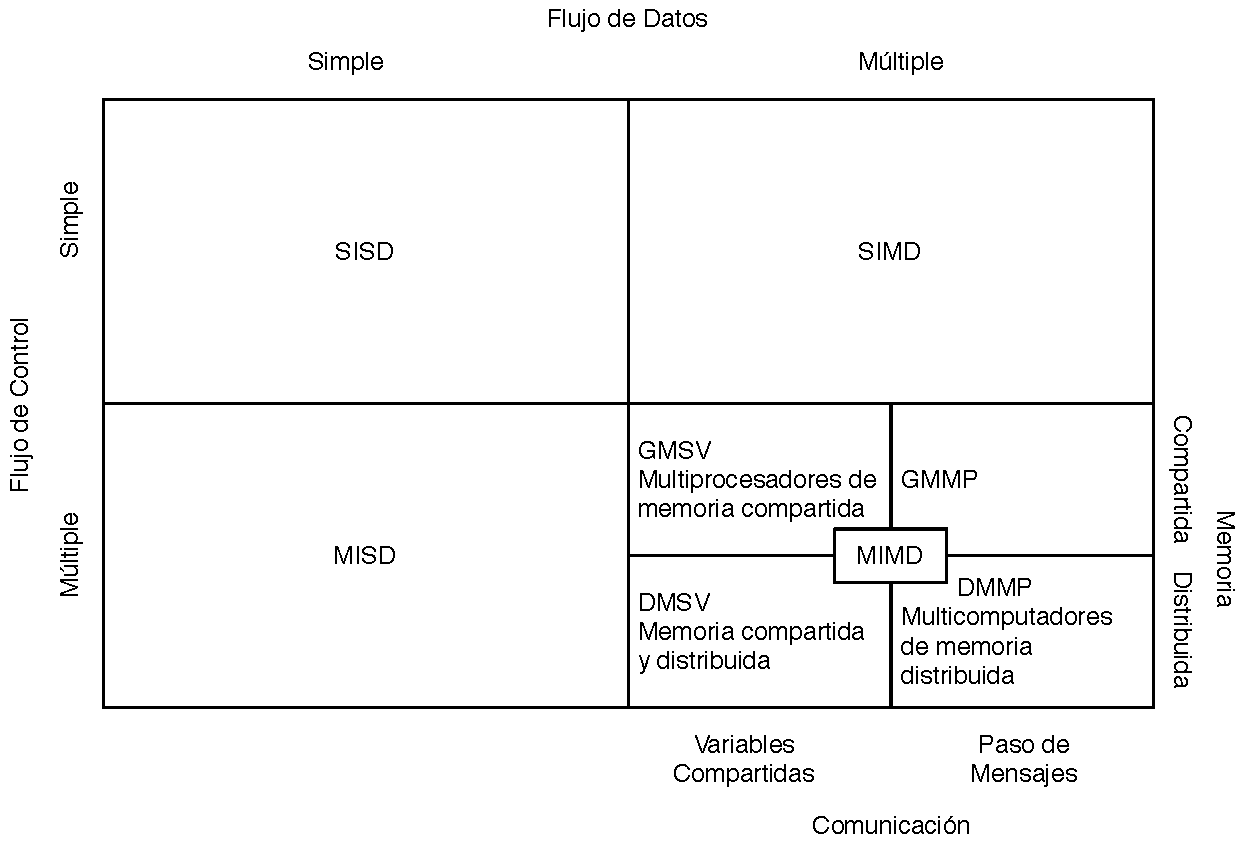
\includegraphics[width=10cm]{cap2/flynn.pdf}
\caption{La clasificaci�n de Flynn-Johnson de los sistemas inform�ticos}
\label{fig:flynn}
\end{center}
\end{figure}


En 1996, M. J. Flynn propuso una clasificaci�n en 4 categor�as de los sistemas
inform�ticos bas�ndose en el flujo de datos y el flujo de instrucciones; esta
clasificaci�n se ha convertido en un est�ndar y se usa en muchos �mbitos. Flynn
acu�� cuatro abreviaturas para estas 4 clases: SISD, SIMD, MISD y MIMD,
bas�ndose en el n�mero de flujos de instrucciones (simple o m�ltiple) y en los
flujos de datos (simples o m�ltiples) \cite{Flyn96}, Fig.
\ref{fig:flynn}.

Una breve descripci�n de cada tipo \cite{bastida}, \cite{pardo02}:
\begin{enumerate}
\item \textbf{SISD.} (Single Instruction stream, Single Data stream) Flujo �nico
de instrucciones y flujo �nico de datos. Este es el concepto de arquitectura serie
de Von Neumann donde, en cualquier momento, s�lo se est� ejecutando una �nica
instrucci�n. A menudo a los SISD se les conoce como computadores serie escalares. Todas las 
m�quinas SISD poseen un registro simple que se llama contador de programa 
que asegura la ejecuci�n en serie del programa. Conforme se van leyendo las 
instrucciones de la memoria, el contador de programa se actualiza para que
apunte a la siguiente instrucci�n a procesar en serie. Pr�cticamente ning�n
sistema puramente SISD se fabrica hoy en d�a ya que la mayor�a de procesadores
modernos incorporan alg�n grado de paralelismo como es la segmentaci�n de
instrucciones o la posibilidad de lanzar dos instrucciones al mismo tiempo (superescalares). 
Fig.\ref{figsisd}.
\begin{figure}[hp]
\begin{center}
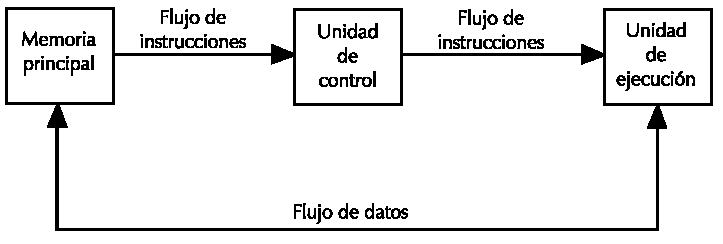
\includegraphics[width=9cm]{cap2/sisd.pdf}
\caption{Organizaci�n Simple Instruction Simple Data (SISD)}
\label{figsisd}
\end{center}
\end{figure}

\item \textbf{SIMD.} (Single Instruction stream, Multiple Data stream) Flujo de
instrucci�n simple y flujo de datos m�ltiple. Esto significa que una �nica
instrucci�n es aplicada sobre diferentes datos al mismo tiempo. En las m�quinas de este tipo, varias unidades 
de procesado diferentes son invocadas por una �nica unidad de control. Al igual 
que las MISD, las SIMD soportan procesamiento vectorial (matricial) asignando 
cada elemento del vector a una unidad funcional diferente para procesamiento 
concurrente. Por ejemplo, el c�lculo de la paga para cada trabajador en una
empresa, es repetir la misma operaci�n sencilla para cada trabajador; si se
dispone de un arquitectura SIMD esto se puede calcular en paralelo para cada
trabajador. Por esta facilidad en la paralelizaci�n  de vectores de datos (los
trabajadores formar un vector) se les llama tambi�n procesadores vectoriales. 
, Fig. \ref{figsimd}.
\begin{figure}
\begin{center}
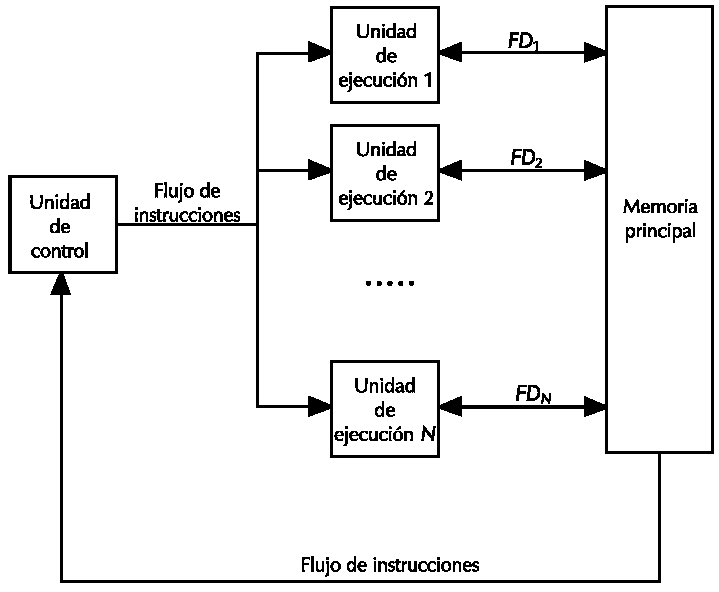
\includegraphics[width=9cm]{cap2/simd.pdf}
\caption{Organizaci�n Simple Instruction Multiple Data (SIMD)}
\label{figsimd}
\end{center}
\end{figure}

\item \textbf{MISD.} 
(Multiple Instruction stream, Single Data stream) Flujo m�ltiple de
instrucciones y �nico flujo de datos. Esto significa que varias instrucciones
act�an sobre el mismo y �nico trozo de datos. Este tipo de m�quinas se pueden 
interpretar de dos maneras. Una es considerar la clase de maquinas que
necesitando unidades  de procesamiento diferentes recibieran instrucciones
distintas operando sobre
los mismos datos. Esta clase de arquitectura ha sido clasificada por numerosos
arquitectos de computadores como impracticable o imposible, y en estos momentos no 
existen ejemplos que funcionen siguiendo este modelo. Otra forma de interpretar 
los MISD es como una clase de m�quinas donde un mismo flujo de datos fluye 
a trav�s de numerosas unidades de proceso. Arquitecturas altamente segmentadas, 
como los procesadores vectoriales, son clasificados a 
menudo bajo este tipo de m�quinas. Las arquitecturas segmentadas, o
encauzadas, realizan el procesamiento vectorial a trav�s de una serie de etapas, cada
una ejecutando una funci�n  particular produciendo un resultado intermedio. La
raz�n por la cual dichas arquitecturas son clasificadas como MISD es que los elementos 
de un vector pueden ser considerados como pertenecientes al mismo dato, y todas 
las etapas del flujo representan m�ltiples instrucciones que son aplicadas
sobre ese vector, Fig. \ref{figmisd}.
\begin{figure}[ht]
\begin{center}
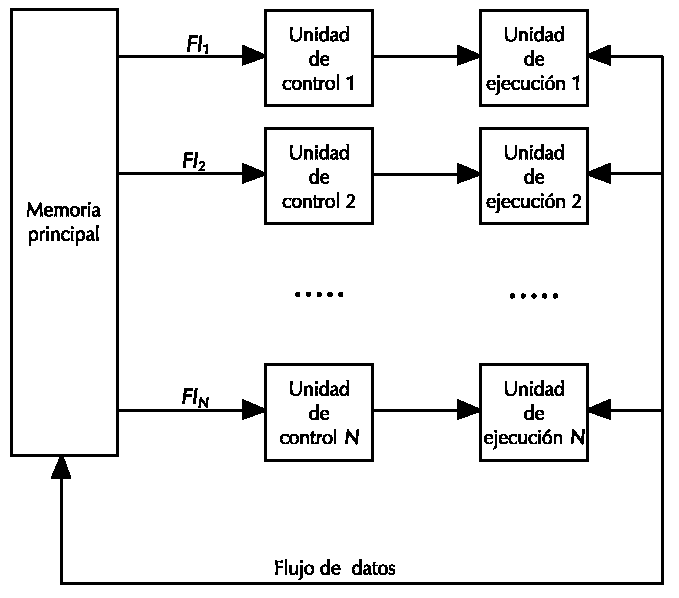
\includegraphics[width=9cm]{cap2/misd.pdf}
\caption{Organizaci�n Multiple Instruction Simple Data (MISD)}
\label{figmisd}
\end{center}
\end{figure}
\afterpage{\clearpage}
\item \textbf{MIMD.} (Multiple Instruction stream, Multiple Data stream) Flujo
de instrucciones m�ltiple y flujo de datos m�ltiple. Son m�quinas que poseen varias unidades
de proceso en las cuales se pueden realizar m�ltiples instrucciones sobre datos
diferentes de forma simult�nea. Las MIMD son las m�s complejas, pero son tambi�n 
las que potencialmente ofrecen una mayor eficiencia en la ejecuci�n concurrente
o paralela. Aqu� la concurrencia implica que no solo hay varios
procesadores operando simult�neamente, sino que adem�s hay varios programas
(procesos) ejecut�ndose tambi�n al mismo tiempo, Fig. \ref{figmimd}.
\begin{figure}[h]
\begin{center}
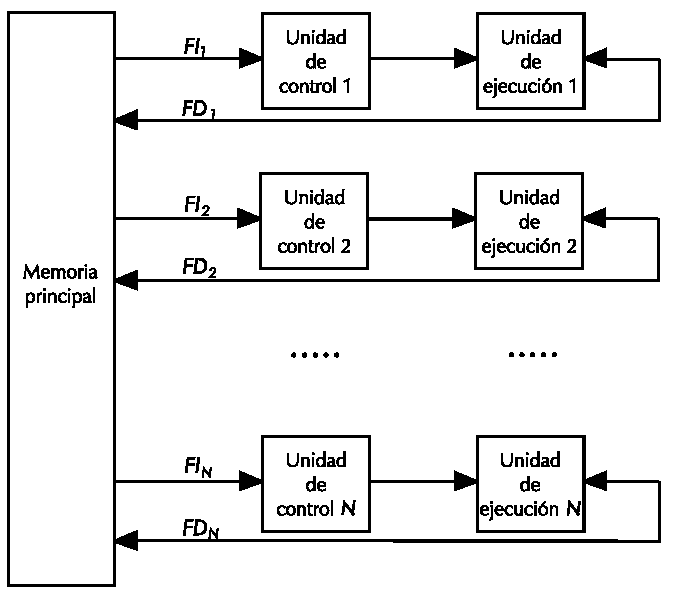
\includegraphics[width=9cm]{cap2/mimd.pdf}
\caption{Organizaci�n Multiple Instruction Multiple Data (MIMD)} 
\label{figmimd}
\end{center}
\end{figure}
\end{enumerate}

\subsection{Otras clasificaciones}
La clasificaci�n de Flynn ha demostrado funcionar bastante bien para la
tipificaci�n de sistemas, y se ha venido usando desde d�cadas por la mayor�a de
la comunidad inform�tica. Sin embargo, los avances en tecnolog�a y diferentes
topolog�as, han llevado a sistemas que no son tan f�ciles de clasificar dentro de los 4 tipos
de Flynn. Por ejemplo, las arquitecturas h�bridas. Para solucionar esto se han
propuesto otras clasificaciones, donde los tipos SIMD y MIMD de Flynn se suelen conservar, pero
que sin duda no han tenido el �xito de la de Flynn.

La figura \ref{figclascompleta} muestra una clasificaci�n ampliada que incluye alguno de los avances 
en arquitecturas de computadores en los �ltimos a�os. No obstante, tampoco
pretende ser una caracterizaci�n completa de todas las arquitecturas paralelas
existentes. 
\begin{figure}[h]
\begin{center}
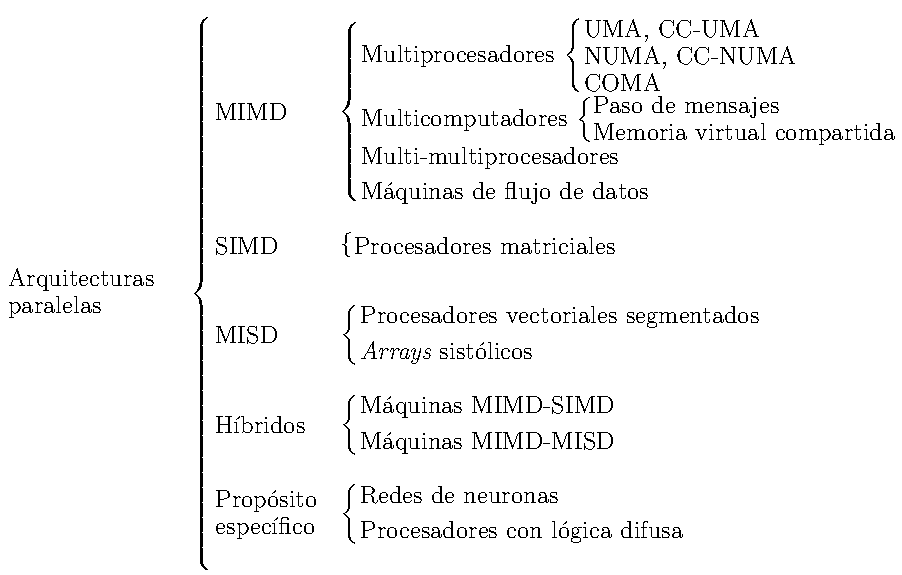
\includegraphics[width=9cm]{cap2/clascompleta.pdf}
\caption{Clasificaci�n extendida de las arquitecturas paralelas}
\label{figclascompleta}
\end{center}
\end{figure}

\subsubsection{Multiprocesadores}
De todas estas arquitecturas se va a hacer una menci�n especial a los
\textbf{multiprocesadores}. Un multiprocesador se puede ver como un computador
paralelo compuesto por varios procesadores interconectados que pueden compartir un mismo sistema de memoria.
Los procesadores se pueden configurar para que ejecute cada uno una parte de un
programa o varios programas al mismo tiempo. 

Dado que los multiprocesadores comparten los diferentes m�dulos de memoria, 
pudiendo acceder varios procesadores a un mismo m�dulo, a los multiprocesadores
tambi�n se les llama sistemas de memoria compartida. Dependiendo de la forma en
que los procesadores comparten la memoria, podemos hacer una subdivisi�n de los
multiprocesadores: 
\begin{itemize}
\item\textbf{UMA.} (Uniform Memory Access) En un modelo de Memoria de Acceso Uniforme, la 
memoria f�sica est� uniformemente compartida por todos los procesadores. Esto 
quiere decir que todos los procesadores tienen el mismo tiempo de acceso a todas 
las palabras de memoria. Cada procesador puede tener su cach� privada, y los 
perif�ricos son tambi�n compartidos de alguna manera. A estos computadores se les suele 
llamar sistemas fuertemente acoplados dado el alto grado de compartici�n de los recursos. 
La red de interconexi�n toma la 
forma de bus com�n, conmutador cruzado, o una red multietapa.
Cuando todos los procesadores tienen el mismo acceso a todos los perif�ricos,
el sistema se llama \textit{multiprocesador sim�trico}. En este caso, todos los
procesadores 
tienen la misma capacidad para ejecutar programas, tal como el Kernel o las 
rutinas de servicio de entrada/salida. En un \textit{multiprocesador asim�trico}
, s�lo un subconjunto de los procesadores pueden ejecutar programas. A los que pueden, 
o al que puede ya que muchas veces es s�lo uno, se le llama maestro. Al resto de procesadores 
se les llama procesadores adheridos (attached processors). La figura
\ref{figuma} muestra el modelo UMA de un multiprocesador. 
Es frecuente encontrar arquitecturas de acceso uniforme que adem�s tienen coherencia 
 cach�, a estos sistemas se les suele llamar \textbf{CC-UMA} (Cache-Coherent 
Uniform Memory Access). 
\begin{figure}
\begin{center}
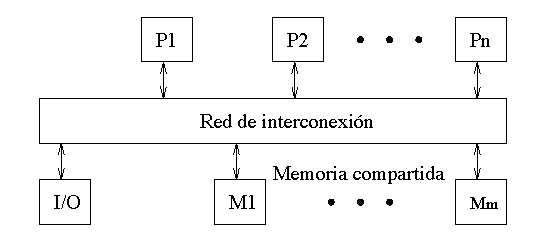
\includegraphics[width=9cm]{cap2/uma.pdf}
\caption{Modelo UMA de multiprocesador}
\label{figuma}
\end{center}
\end{figure}

\item\textbf{NUMA.} Un multiprocesador de tipo NUMA es un sistema de memoria
compartida donde el tiempo de acceso var�a seg�n el lugar donde se encuentre localizado
el acceso. La figura \ref{fignuma} muestra una posible configuraci�n de tipo NUMA, 
donde toda la memoria es compartida pero local a cada m�dulo procesador. Otras posibles 
configuraciones incluyen los sistemas basados en agrupaciones (clusters) de
sistemas como el de la figura que se comunican a trav�s de otra red de
comunicaci�n que puede incluir una memoria compartida global.

La ventaja de estos sistemas es que el acceso a la memoria local es m�s r�pido
que en los UMA aunque un acceso a memoria no local es m�s lento. Lo que se 
intenta es que la memoria utilizada por los procesos que ejecuta cada
procesador, se encuentre en la memoria de dicho procesador para que los accesos
sean lo m�s locales que se pueda.

Aparte de esto, se puede a�adir al sistema una memoria de acceso global. En 
este caso se dan tres posibles patrones de acceso. El m�s r�pido es el acceso
a memoria local. Le sigue el acceso a memoria global. El m�s lento es el acceso
a la memoria del resto de m�dulos.

Al igual que hay sistemas de tipo CC-UMA, tambi�n existe el modelo de acceso 
a memoria no uniforme con coherencia de cach� \textbf{CC-NUMA} (Cache-Coherent 
Non-Uniform Memory Access) que consiste en memoria compartida distribuida y 
directorios de cache.

\begin{figure}
\begin{center}
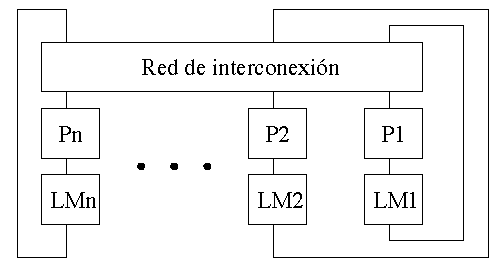
\includegraphics[width=9cm]{cap2/numa.pdf}
\caption{Modelo NUMA de multiprocesador}
\label{fignuma}
\end{center}
\end{figure}

\item\textbf{COMA.} (Cache Only Memory Access) Un multiprocesador que solo use
cach� como memoria es considerado de tipo COMA. La figura \ref{figcoma} muestra
el modelo COMA de multiprocesador. En realidad, el modelo COMA es un caso especial del 
NUMA donde las memorias distribuidas se convierten en cach�s. No hay jerarqu�a de 
memoria en cada m�dulo procesador. Todas las cach�s forman un mismo espacio 
global de direcciones. El acceso a las cach�s remotas se realiza a trav�s de los 
directorios distribuidos de las cach�s. Dependiendo de la red de interconexi�n 
empleada, se pueden utilizar jerarqu�as en los directorios para ayudar en la
localizaci�n de copias de bloques de cach�. El emplazamiento inicial de datos no es 
cr�tico puesto que el dato acabar� estando en el lugar en que se use m�s. 
\begin{figure}
\begin{center}
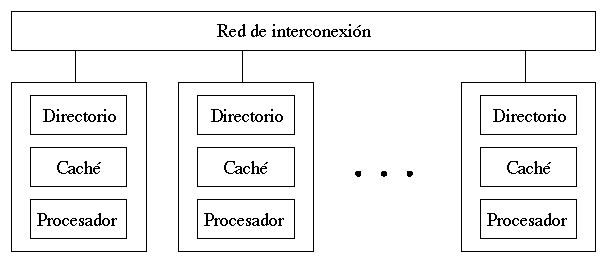
\includegraphics[width=9cm]{cap2/coma.pdf}
\caption{Modelo COMA de multiprocesador}
\label{figcoma}
\end{center}
\end{figure}
\end{itemize}

\section{El benchmark TPC-C}

Los \textbf{benchmarks} producidos por el TPC son est�ndares industriales; el
TPC distribuye gratuitamente las especificaciones de estas pruebas, por lo que
cualquiera es libre de implementar y publicar un resultado TPC. Sin embargo, hay
que aclarar que todos los datos de la implementaci�n tienen que ser enviados al
TPC para ser revisados, ya que si un fabricante realiza su prueba TPC de manera
incorrecta o de una manera parcial y subjetiva deber� retirar los resultados y
no los podr� usar p�blicamente, por lo que estas reglas protegen a los usuarios
de resultados falsos o confusos a la vez que mantienen la credibilidad de los
resultados de un benchmark TPC.
 
Las especificaciones de los \textit{benchmarks}  TPC son documentos de unas
30-50 p�ginas que definen como configurar, ejecutar y documentar un benchmark
TPC; adem�s y aparte de las pruebas de rendimiento, los benchmarks TPC necesitan
varias pruebas independientes de fiabilidad y seguridad que garanticen a los
usuarios que el sistema que est� siendo probado se asemeje a uno de un entorno
real de producci�n, por lo que normalmente los benchmark TPC son bastante m�s
complejos y requieren de m�s tiempo para implementar que otras pruebas m�s
sencillas que pueden realizarse contra una simple cinta de datos.


\subsection{Caracter�sticas del benchmark TPC-C}
 
El benchmark TPC-C es una carga de trabajo \textit{de procesado de transacciones
en l�nea (OLTP)}; OLTP (online transaction processing) es una clase de trabajo
que facilita y dirige ciertas aplicaciones orientadas a transacciones,
normalmente para entrada y obtenci�n de datos en un gran n�mero de industrias,
como por ejemplo: bancos, pedidos por correo, l�neas �reas, supermercados y
fabricantes.

Esta prueba es una mezcla de transacciones intensivas de s�lo lectura y
actualizaci�n que simulan el trabajo que se puede encontrar en entornos
complejos con aplicaciones OLTP, que suelen tener las siguientes
caracter�sticas:

\begin{itemize}
\item La ejecuci�n simultanea de varios tipos de transacciones que resultan en una gran complejidad.
\item Ejecuci�n de transacciones en l�nea (on-line) y diferidas
\item M�ltiples terminales conectados.
\item Tiempos de ejecuci�n de aplicaciones moderados.
\item Gran cantidad de entrada y salida en disco.
\item Transacciones que cumplan las propiedades ACID 
(Atomic, Consistent, Isolation, and Durable - At�micas, Consistentes, Aisladas 
y Resistentes).
\item Distribuci�n no uniforme del acceso a los datos a trav�s de claves primarias y secundarias.
\item Bases de datos con varias tablas, de varios tama�os, diferentes tipos de atributos y relaciones.
\item Con conflictos entre el acceso a datos y la actualizaci�n.
\end{itemize} 

La m�trica del rendimiento que obtiene el TPC-C es un indicador del rendimiento
a la hora de procesar transacciones midiendo el n�mero de pedidos procesados por
minuto. Varias transacciones son usadas para simular la actividad que se produce
en un negocio a la hora de procesar un pedido, y cada transacci�n est� sujeta a
tiempos de respuesta. Las unidades a utilizar para el rendimiento ser�n
\textit{transacciones por minuto} \textbf{tpmC}. Si se quiere cumplir
estrictamente con el est�ndar TPC-C aparte de los resultados en unidades tpmC,
se debe incluir el precio por cada unidad tpmC as� como la disponibilidad y el
precio de la configuraci�n usada.

Aunque estas especificaciones expresen la implementaci�n en t�rminos de un
modelo de datos relacional con un esquema convencional de bloqueos, la base de
datos puede ser implementada usando cualquier sistema de bases de datos, sistema
de ficheros, o sistema de almacenamiento de datos que proporcione una
implementaci�n funcionalmente equivalente; por lo que aunque en las
especificaciones del est�ndar se digan las palabras ``tabla'', ``fila'' o
``columna'' no implica un uso de un sistema relacional.

A la hora de comparar los resultados obtenidos por un benchmark TPC-C, hay que
indicar que s�lo los resultados de una prueba son comparados con los de otra
prueba si ambas pruebas son conformes a la misma revisi�n del TPC-C; por lo que
aunque la terminolog�a que se extrae del est�ndar pueda parecerse a otros
benchmarks del TPC o de otras entidades, no implica que estos resultados sean
comparables con otros benchmarks.

Este benchmark ofrece un entorno rico que intenta emular muchas aplicaciones
OLTP, aunque no siempre es posible reflejar todo el rango de aplicaciones OLTP
as� como sus necesidades, es necesario indicar que los resultados obtenidos por
este benchmark en un sistema pueden no acercarse a las necesidades reales de un
sistema/aplicaci�n concreto debido a que el TPC-C no se aproxima a esas
necesidades. Con esto se puede afirmar que el rendimiento obtenido en un sistema
aplicando este benchmark no se aplica necesariamente a otras cargas de trabajo o
entornos, por lo que no se recomienda extrapolar los resultados m�s all� del
sistema donde fueron obtenidos.

Los resultados del benchmark dependen mucho de la carga de trabajo, necesidades de la aplicaci�n y dise�o e implementaci�n del sistema, por lo que el rendimiento relativo variar� como resultado de estos y otros factores; por lo tanto, TPC-C no debe ser usado como un sustituto para sacar resultados de una aplicaci�n concreta, y mucho menos cuando contemplamos aspectos cr�ticos como planificaci�n de capacidad o evaluaci�n de un producto final.

\subsection{Algunas pautas para la implementaci�n}
Como ya dijimos el objetivo de las pruebas TPC es obtener datos de rendimiento relevantes y objetivos para la industria, para alcanzar estos objetivos hace falta que las pruebas, los sistemas y las tecnolog�as empleadas:
\begin{itemize}
\item Est�n disponibles al p�blico.
\item Contemplen aspectos importantes en el �rea de negocio que intenta simularse.
\item Exista un n�mero de usuarios importante que implementar�a lo que se intenta simular.
\end{itemize} 

Estas caracter�sticas se usan para saber si una implementaci�n particular es un benchmark especial, y son muy generales, se pueden listar otras caracter�sticas m�s concretas que pueden indicar en mayor o menor medida si el benchmark que se realiza es especifico:

\begin{itemize}
\item �Est� la implementaci�n p�blicamente disponible, documentada y soportada?
\item La implementaci�n tiene restricciones importantes o su uso est� muy
limitado m�s all� del TPC-C.
\item La implementaci�n o parte de ella se integra muy mal en un producto final.
\item La implementaci�n se aprovecha de la naturaleza limitada del benchmark TPC-C de tal manera que no puede ser aplicada generalmente al entorno que intenta simular.
\item El fabricante del sistema no aprueba la implementaci�n.
\item La implementaci�n necesita de ciertos aspectos excepcionales por parte del usuario final, programador o administrador.
\item La implementaci�n no se usa por usuarios finales en el �rea de mercado que el benchmark simula.
\end{itemize} 

No es necesario que todas estas condiciones sean evitadas/cumplidas para que una implementaci�n pueda tildarse de espec�fica, pero ayudan en menor o mayor grado a clasificarla.


\chapter{An�lisis del sistema TPC-C}
\section{Requisitos}\label{sec:requisitos}
Normalmente en un an�lisis de requisitos se recogen las necesidades del proyecto
y se organizan de tal manera que se obtienen una serie de requisitos funcionales y
no funcionales. En el caso de un est�ndar ya escrito, los requisitos vienen ya
descritos en el documento del est�ndar.

Pueden existir requisitos que no se vayan a implementar; pero aqu� se plantear�n
y se analizar�n las especificaciones del benchmark TPC-C, por lo que puede que
haya ciertos aspectos que aunque debieran de estar en un dise�o se presenten en
este an�lisis.

El an�lisis est� realizado en base a las especificaciones del \textit{TPC
benchmark C} con versi�n 5.2 de diciembre del 2003, que se pueden encontrar en
\url{http://www.tpc.org}

\subsection{Descripci�n general}
El benchmark TCP-C se centra en analizar el rendimiento de entornos OLTP, por lo
que se centra en un ejemplo lo m�s general posible basado en la actividad de una
 empresa de distribuci�n a gran escala, con el prop�sito de analizar las
caracter�sticas principales de una aplicaci�n de este tipo a la vez que nos
centramos en un conjunto m�s reducido de operaciones, y evitar analizar ciertas
operaciones que son poco utilizadas o los recursos que utilizan no son de
inter�s.

La empresa que vamos a analizar con este benchmark es un distribuidor mayorista
que dispone de una serie de almacenes distribuidos geogr�ficamente; cada almac�n
da servicio a 10 zonas, y en cada zona se sirve a 3000 clientes. Tambi�n, un
almac�n debe de controlar las existencias de 100.000 productos vendidos por la
empresa.

Los clientes contactan con la empresa para realizar pedidos o consultar su
estado; estos pedidos est�n compuestos de una media de 10 elementos distintos, y
de un 1\% de estos elementos no se dispone de existencias en el almacen local
teni�ndose que encargar a otro almac�n. Este sistema tambi�n se usa para anotar
los pagos de los clientes, procesar los pedidos y observar las existencias de
los productos para anticiparse a la escasez de estos.

\subsection{Entidades y relaciones de la base de datos}
Los componentes de la base de datos del TPC-C son 9 tablas relacionadas entre
si, cuya estructura podemos observar en la figura \ref{figer}. No se indican los
atributos de cada entidad ya que ser�n detallados m�s tarde junto con el tipo de
atributo y la clave de la entidad.

\begin{figure}
\begin{center}
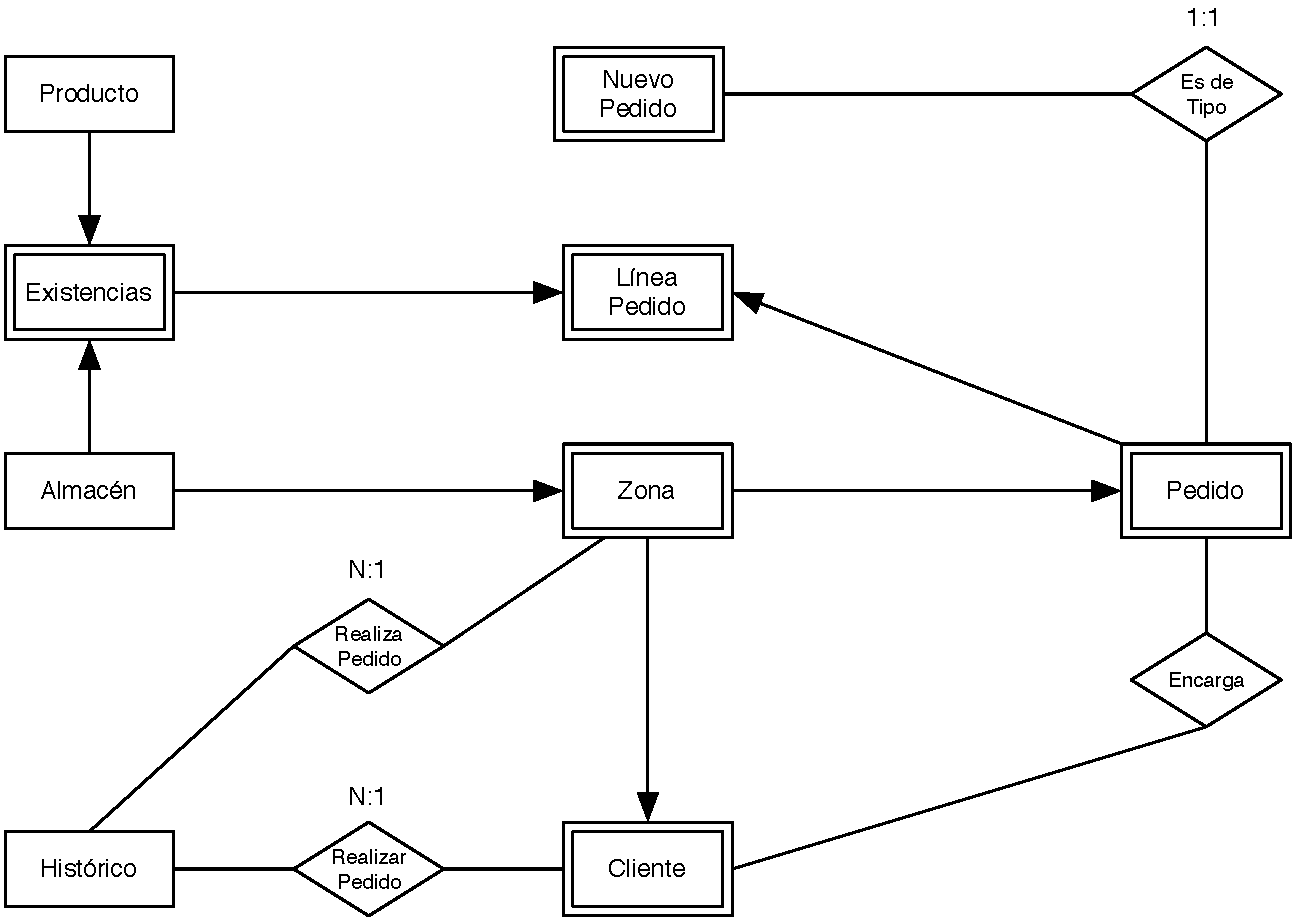
\includegraphics[width=\textwidth]{cap3/er.pdf}
\caption{Diagrama entidad-relaci�n del sistema de almacenamiento}
\label{figer}
\end{center}
\end{figure}
\subsubsection{Relaciones}
Como se puede ver la mayor�a de relaciones son de entidad d�bil, y muchas
entidades dependen de otras; se puede decir que las �nicas entidades que siempre
perduran son los almacenes y los productos, as� como el hist�rico que es
simplemente un historial de operaciones realizadas.
\begin{itemize}
\item Un \textit{almac�n} est� compuesto de 10 \textit{zonas}, por lo que zona
es entidad d�bil de almac�n.
\item Una \textit{zona} tiene asociados \textit{clientes} y \textit{pedidos};
como antes, clientes y pedidos se convierten en entidades d�biles que dependen
de zona.
\item Un \textit{cliente encarga pedidos} y esos pedidos los encarga en una zona
determinada (la suya u otra) por lo que en el \textit{hist�rico} se almacenan
tanto los datos del cliente que realiza el pedido como los de la zona donde se
ha realizado el pedido.
\item Un \textit{pedido} puede ser de tipo \textit{nuevo pedido}, que indica que
aun no se ha enviado al cliente.
\item El \textit{pedido} se compone de m�ltiples \textit{l�neas de pedido}, por
lo que dichas l�neas son entidades d�biles de pedido.
\item Cada \textit{l�nea de pedido} indica un producto y su cantidad pero se
relaciona con \textit{productos} a trav�s de \textit{existencias}.
\item Las \textit{existencias} indican la cantidad de cada \textit{producto} que
resta en un \textit{almac�n}.
\end{itemize}

\subsubsection{Tipos de atributos}
Los tipos de atributos empleados para describir los atributos de las entidades de la base de datos son los siguientes:
\begin{itemize}
\item\textbf{N Identificadores �nicos}: Un atributo que es capaz de almacenar
cualquier identificador (ID) dentro de un conjunto m�nimo de N identificadores
�nicos, independientemente de la representaci�n real del atributo: binario,
decimal, letras, etc.
\item\textbf{Texto de tama�o variable, N}: El atributo debe ser capaz de
almacenar cualquier cadena de caracteres de longitud variable con una longitud
m�xima de N caracteres. Si el atributo es almacenado como una cadena de longitud
fija, y su longitud es m�s corta que N, se debe rellenar con espacios.
\item\textbf{Texto de tama�o fijo, N}: El atributo debe ser capaz de almacenar
cualquier cadena de caracteres de longitud N fija.
\item\textbf{Fecha y hora}: El atributo es capaz de almacenar una fecha entre el
1 de Enero de 1900 y el 31 de Diciembre de 2100 con una resoluci�n de al menos
un segundo.
\item\textbf{Numero, N d�gitos}: El atributo debe ser capaz de almacenar
cualquier valor de N d�gitos decimales. Para el caso de valores monetarios,
tiene que asegurarse la precisi�n en los decimales de la unidad m�s peque�a de
dinero: en el caso de euros, la precisi�n m�nima est� en 1 c�ntimo.
\item\textbf{Nulo}: significa fuera del rango de los valores aceptados para un
atributo conocido adem�s de ser siempre el mismo valor para ese atributo. 
\end{itemize} 

En las tablas, los atributos tendr�n una de estas definiciones, para definir que son capaces de contener; esto no implica ninguna dependencia con la implementaci�n f�sica a utilizar m�s tarde cuando se implemente el sistema.

\subsubsection{Entidades}
Dado el diagrama relacional anterior, y listados los tipos de atributos de los
que disponemos, vamos a listar todas las entidades con sus atributos y sus
campos clave.
% Definicion de las tablas sql
\newlength{\lineaparrafo}
\setlength{\lineaparrafo}{\linewidth}
\addtolength{\lineaparrafo}{-15.1pt}
\newenvironment{tablasql}
	{\tabularx{\lineaparrafo}{|l|l|X|}
	\hline
	\textbf{Nombre del campo} & \textbf{Tipo de campo} & \textbf{Comentarios} \\
	\hline  \hline}
	{\endtabularx}

\paragraph{Almac�n (WAREHOUSE)}
Ver cuadro \ref{tab:desc-almacen}.
\begin{table}
\begin{tablasql}
W\_ID & 2*W identificadores �nicos & Siendo W el n�mero de almacenes\\
W\_NAME & Texto de tama�o variable, 10 & \\
W\_STREET\_1 & Texto de tama�o variable, 20 & \\
W\_STREET\_2 & Texto de tama�o variable, 20 & \\
W\_CITY & Texto de tama�o variable, 20 &\\
W\_STATE & Texto de tama�o fijo, 2 &\\
W\_ZIP & Texto de tama�o fijo 9 &\\
W\_TAX & N�mero, 4 d�gitos & Impuestos de ventas \\
W\_YTD & N�mero,  12 d�gitos & Balance total anual \\
\hline \hline
\multicolumn{3}{|l|}{Clave primaria: W\_ID} \\
\hline 
\end{tablasql} 
\caption{Descripci�n de la tabla Almac�n}
\label{tab:desc-almacen}
\end{table}

\paragraph{Zona (DISTRICT)}
Ver cuadro \ref{tab:desc-zona}.
\begin{table}
\begin{tablasql}
D\_ID & 20 identificadores �nicos & 10 poblados por almac�n\\
D\_W\_ID & 2*W identificadores �nicos&\\
D\_NAME & Texto de tama�o variable, 10&\\
D\_STREET\_1 &  Texto de tama�o variable, 20&\\
D\_STREET\_2 &Texto de tama�o variable, 20&\\
D\_CITY & Texto de tama�o variable, 20&\\
D\_STATE & Texto de tama�o fijo, 2 &\\
D\_ZIP & Texto de tama�o fijo 9 &\\
D\_TAX & N�mero, 4 d�gitos & Impuestos de ventas \\
D\_YTD & N�mero,  12 d�gitos & Balance total anual\\
D\_NEXT\_O\_ID & 10.000.000 identificadores �nicos&Siguiente n�mero de orden disponible\\
\hline \hline
\multicolumn{3}{|l|}{Clave primaria: D\_ID, D\_W\_ID} \\
\multicolumn{3}{|l|}{(D\_W\_ID) clave for�nea de Almac�n (W\_ID)}\\
\hline
\end{tablasql}
\caption{Descripci�n de la tabla Zona}
\label{tab:desc-zona}
\end{table}

\paragraph{Cliente (CUSTOMER)}
Ver cuadro \ref{tab:desc-cliente}.
\begin{table}
\begin{tablasql}
C\_ID     & 96.000 identificadores �nicos & 3.000 poblados por zona\\
C\_D\_ID  & 20 identificadores �nicos & \\
C\_W\_ID  & 2*W identificadores �nicos & \\
C\_FIRST  & Texto de tama�o variable, 16 & \\
C\_MIDDLE & Texto de tama�o fijo, 2 & \\
C\_LAST   & Texto de tama�o variable, 16 & \\
C\_STREET\_1 & Texto de tama�o variable, 20 & \\
C\_STREET\_2 & Texto de tama�o variable, 20 & \\
C\_CITY  & Texto de tama�o variable, 20 & \\
C\_STATE & Texto de tama�o fijo, 2 & \\
C\_ZIP   & Texto de tama�o fijo, 9 & \\
C\_PHONE & Texto de tama�o fijo 16 & \\
C\_SINCE & Fecha y hora & \\
C\_CREDIT        & Texto de tama�o fijo 2 & ``GC''=bueno, ``BC''=malo \\
C\_CREDIT\_LIM   & N�mero, 12 d�gitos & \\
C\_DISCOUNT      & N�mero, 4 d�gitos & \\
C\_BALANCE       & N�mero con signo, 12 d�gitos & \\
C\_YTD\_PAYMENT  & N�mero, 12 d�gitos & \\
C\_PAYMENT\_CNT  & N�mero, 4 d�gitos & \\
C\_DELIVERY\_CNT & N�mero, 4 d�gitos & \\
C\_DATA          & Texto de tama�o variable, 500 & Informaci�n variada \\
\hline \hline
\multicolumn{3}{|l|}{Clave primaria: C\_W\_ID, C\_D\_ID, C\_ID} \\
\multicolumn{3}{|l|}{(C\_W\_ID, C\_D\_ID) clave for�nea de Zona (D\_W\_ID, D\_ID)}\\
\hline
\end{tablasql}
\caption{Descripci�n de la tabla Cliente}
\label{tab:desc-cliente}
\end{table}

\paragraph{Hist�rico (HISTORY)}
Ver cuadro \ref{tab:desc-historico}.
\begin{table}
\begin{tablasql}
H\_C\_ID    & 96.000 identificadores �nicos & \\
H\_C\_D\_ID & 20 identificadores �nicos & \\  
H\_C\_W\_ID & 2*W identificadores �nicos & \\
H\_D\_ID  & 20 identificadores �nicos & \\
H\_W\_ID  & 2*W identificadores �nicos & \\
H\_DATE   & Fecha y hora & \\
H\_AMOUNT & Numero, 6 d�gitos & \\
H\_DATA   & Texto de tama�o variable, 24 & Informaci�n variada \\
\hline \hline
\multicolumn{3}{|l|}{Clave primaria: ninguna, en este contexto no es necesario identificar �nicamente a cada tupla.} \\
\multicolumn{3}{|l|}{(H\_C\_W\_ID, H\_C\_D\_ID, H\_C\_ID) clave for�nea de Cliente (C\_W\_ID, C\_D\_ID, C\_ID)}\\
\multicolumn{3}{|l|}{(H\_W\_ID, H\_D\_ID) clave for�nea de Almac�n (D\_W\_ID, D\_ID)}\\
\hline
\end{tablasql}
\caption{Descripci�n de la tabla Hist�rico}
\label{tab:desc-historico}
\end{table}

\paragraph{Nuevo-Pedido (NEW-ORDER)}
Ver cuadro \ref{tab:desc-nuevopedido}.
\begin{table}
\begin{tablasql}
NO\_O\_ID & 10.000.000 identificadores �nicos & \\  
NO\_D\_ID & 20 identificadores �nicos & \\  
NO\_W\_ID & 2*W identificadores �nicos & \\
\hline \hline
\multicolumn{3}{|l|}{Clave primaria: NO\_W\_ID, NO\_D\_ID, NO\_O\_ID} \\
\multicolumn{3}{|l|}{(NO\_W\_ID, NO\_D\_ID, NO\_O\_ID) clave for�nea de Pedido (O\_W\_ID, O\_D\_ID, O\_ID)}\\
\hline
\end{tablasql}
\caption{Descripci�n de la tabla Nuevo-Pedido}
\label{tab:desc-nuevopedido}
\end{table}

\paragraph{Pedido (ORDER)}
Ver cuadro \ref{tab:desc-pedido}.
\begin{table}
\begin{tablasql}
O\_ID    & 10.000.000 identificadores �nicos & \\
O\_D\_ID &20 identificadores �nicos & \\
O\_W\_ID &2*W identificadores �nicos & \\
O\_C\_ID &96.000 identificadores �nicos & \\
O\_ENTRY\_D & Fecha y hora & \\
O\_CARRIER\_ID &10 identificadores �nicos o nulo & \\  
O\_OL\_CNT & N�mero, 2 d�gitos & De 5 a 15 l�neas de pedido \\ 
O\_ALL\_LOCAL & N�mero, 1 d�gito & \\
\hline \hline
\multicolumn{3}{|l|}{Clave primaria: O\_W\_ID, O\_D\_ID, O\_ID} \\
\multicolumn{3}{|l|}{(O\_W\_ID, O\_D\_ID, O\_C\_ID) clave for�nea de (C\_W\_ID, C\_D\_ID, C\_ID)}\\
\hline
\end{tablasql}
\caption{Descripci�n de la tabla Pedido}
\label{tab:desc-pedido}
\end{table}

\paragraph{L�nea-Pedido (ORDER-LINE)}
Ver cuadro \ref{tab:desc-lineapedido}.
\begin{table}
\begin{tablasql}
OL\_O\_ID  & 10.000.000 identificadores �nicos & \\ 
OL\_D\_ID  & 20 identificadores �nicos & \\  
OL\_W\_ID  & 2*W identificadores �nicos & \\  
OL\_NUMBER & 15 identificadores �nicos & \\ 
OL\_I\_ID  & 200.000 identificadores �nicos & \\
OL\_SUPPLY\_W\_ID & 2*W identificadores �nicos & \\  
OL\_DELIVERY\_D   & Fecha y hora o nulo & \\
OL\_QUANTITY      & N�mero, 2 d�gitos & \\  
OL\_AMOUNT        & N�mero, 6 d�gitos  & \\
OL\_DIST\_INFO    & Texto de tama�o fijo, 24 & \\  
\hline \hline
\multicolumn{3}{|l|}{Clave primaria: OL\_W\_ID, OL\_D\_ID, OL\_O\_ID, OL\_NUMBER} \\
\multicolumn{3}{|l|}{(OL\_W\_ID, OL\_D\_ID, OL\_O\_ID) clave for�nea de Pedido (O\_W\_ID, O\_D\_ID, O\_ID)}\\
\multicolumn{3}{|l|}{(OL\_SUPPLY\_W\_ID, OL\_I\_ID) clave for�nea de Existencias (S\_W\_ID, S\_I\_ID)}\\
\hline
\end{tablasql}
\caption{Descripci�n de la tabla L�nea-Pedido}
\label{tab:desc-lineapedido}
\end{table}

\paragraph{Producto (ITEM)}
Ver cuadro \ref{tab:desc-producto}.
\begin{table}
\begin{tablasql}
I\_ID     & 200.000 identificadores �nicos & Poblado con 100.000 productos \\ 
I\_IM\_ID & 200.000 identificadores �nicos & Identificador de imagen asociada \\ 
I\_NAME   & Texto de tama�o variable, 24 & \\
I\_PRICE  & N�mero, 5 d�gitos  & \\
I\_DATA   & Texto de tama�o variable, 50 & Nombre de la marca \\
\hline \hline
\multicolumn{3}{|l|}{Clave primaria: I\_ID} \\
\hline
\end{tablasql}
\caption{Descripci�n de la tabla Producto}
\label{tab:desc-producto}
\end{table}

\paragraph{Existencias (STOCK)}
Ver cuadro \ref{tab:desc-existencias}.
\begin{table}
\begin{tablasql}
S\_I\_ID    & 200.000 identificadores �nicos & 100.000 poblados por almac�n \\ 
S\_W\_ID    & 2*W identificadores �nicos & \\
S\_QUANTITY & N�mero, 4 d�gitos  & \\
S\_DIST\_01 & Texto de tama�o variable, 24 & \\
S\_DIST\_02 & Texto de tama�o variable, 24 & \\
S\_DIST\_03 & Texto de tama�o variable, 24 & \\
S\_DIST\_04 & Texto de tama�o variable, 24 & \\
S\_DIST\_05 & Texto de tama�o variable, 24 & \\
S\_DIST\_06 & Texto de tama�o variable, 24 & \\
S\_DIST\_07 & Texto de tama�o variable, 24 & \\
S\_DIST\_08 & Texto de tama�o variable, 24 & \\
S\_DIST\_09 & Texto de tama�o variable, 24 & \\
S\_DIST\_10 & Texto de tama�o variable, 24 & \\
S\_YTD & N�mero, 8 d�gitos & \\  
S\_ORDER\_CNT & N�mero, 4 d�gitos & \\ 
S\_REMOTE\_CNT & N�mero, 4 d�gitos & \\
S\_DATA & Texto de tama�o variable, 50 & Informaci�n variada \\ 
\hline \hline
\multicolumn{3}{|l|}{Clave primaria: S\_W\_ID, S\_I\_ID} \\
\multicolumn{3}{|l|}{(S\_W\_ID) clave for�nea de Almac�n (W\_ID)}\\
\multicolumn{3}{|l|}{(S\_I\_ID) clave for�nea de Producto (I\_ID)}\\
\hline
\end{tablasql}
\caption{Descripci�n de la tabla Existencias}
\label{tab:desc-existencias}
\end{table}

\section{Transacciones}\label{sec:transacciones}
\subsection{Introducci�n}
Vamos a utilizar ciertos t�rminos y funciones estad�sticas que conviene definir
antes de explicar detalladamente qu� trabajos se van a realizar sobre la base de
datos.
\begin{itemize}
\item \textbf{Transacci�n:} Hablamos de transacci�n como la unidad de trabajo de nuestro sistema, aunque cada transacci�n se divide en m�ltiples operaciones en la base de datos.
\item \textbf{Rango:} Especificamos un rango de valores entra a y b como [a..b]
\item \textbf{Elemento aleatorio uniforme:} entre un rango de valores [a..b], como un elemento seleccionado de manera independiente y uniforme entre a y b, ambos incluidos.
\item \textbf{Elemento aleatorio no-uniforme:} tambi�n representado por la
funci�n NURAND(X,a,b), un n�mero aleatorio entre un rango de valores [a..b],
seleccionado de manera no uniforme. La f�rmula utilizada para su c�lculo es:
\texttt{NURAND(A, x, y)=( ((random(0, A) | random(x, y) ) + C) modulo (y - x +
1) ) + x} donde:
	\begin{itemize}
	\item \textbf{a | b} Es la operaci�n l�gica OR entre los bits de a y b.
	\item \textbf{random([a..b])} Es un n�mero aleatorio entre a y b.
	\item \textbf{La constante A} Depende del rango [a..b], cuyo valor ser�:
		\begin{itemize}
		\item Para el rango [0..999], usando en C\_LAST: A=255
		\item Para el rango [0..3000], usando en C\_ID: A=1023
		\item Para el rango [0..100000], usando en OL\_I\_ID: A=8191
		\end{itemize}
	\item \textbf{La constante C} Se encuentra dentro del rango [0..A], se elige aleatoriamente en tiempo de ejecuci�n, y puede ser variada sin alterar el rendimiento, aunque debe usarse la misma constante C durante toda la ejecuci�n de la prueba.
	Las normas para tener una buena constante C, son las siguientes:
		\begin{itemize}
		\item Llamemos C-Load a la constante C usada para generar C\_LAST cuando se pobl� la base de datos.
		\item Llamemos C-Run la constante C usada para generar C\_LAST en ejecuci�n.
		\item Obtenemos el valor C-Delta como el valor absoluto de la diferencia entre C-Load y C-Run.
		\item El valor de C-Delta debe estar en el rango de [65..119] excepto los valores 96 y 112.
		\end{itemize}
	\end{itemize}
\item \textbf{Aplicaci�n:} Es el software que, no formando parte del incluido en el sistema de prueba, sirve para implementar los perfiles de transacci�n que se especifican en el est�ndar TPC-C; desde procedimientos, estructuras hasta restricciones de integridad referencial (seg�n el sistema de almacenamiento que se use).
\item \textbf{Terminal:} Se refiere al dispositivo capaz de mostrar caracteres y de recoger las entradas del usuario; dicho dispositivo no debe tener ning�n conocimiento de la aplicaci�n excepto el formato de los campos y su posici�n en la terminal.
\end{itemize}

\subsection{Nuevo pedido}
La transacci�n de \emph{Nuevo Pedido} consiste en introducir un pedido completo
en el sistema. Es una operaci�n con una carga media de lectura y escritura; y
dado que es una de las m�s frecuentes, es el n�cleo de la carga de trabajo, e
intenta simular un comportamiento de carga variable en un sistema real.
\subsubsection{Datos de entrada}\label{sec:nuevopedido-datosdeentrada}
\begin{itemize}
\item El n�mero de almac�n local (W\_ID) permanece constante durante la transacci�n.
\item El n�mero de la zona (D\_ID) donde realizar el pedido es aleatorio entre [1..10]
\item El n�mero de l�neas de pedido (O\_OL\_CNT) es aleatorio entre [5..15], con
una media de 10 l�neas.
\item Para cada l�nea de pedido:
	\begin {enumerate} 
	\item Se selecciona un n�mero de producto entre 1 y 10000 para OL\_I\_ID con una distribuci�n NURAND(8191,1,100000).
	\item Para el almac�n que provee ese producto (OL\_SUPPLY\_W\_ID), el
	99\% de las veces es el almac�n local, pero un 1\% es otro almac�n
	distinto. Esto se puede solucionar f�cilmente con un n�mero aleatorio
	entre [1..100], de tal manera que si ese n�mero es 1, se escoja un
	almac�n local (OL\_SUPPLY\_W\_ID=W\_ID) y en el resto de casos el
	almac�n remoto (OL\_SUPPLY\_W\_ID es aleatorio entre los almacenes
	restantes).
	\item Una cantidad de producto (OL\_QUANTITY) es seleccionada aleatoriamente entre [1 ..10].
	\end{enumerate}
\item Una fecha para el pedido (O\_ENTRY\_D), usando la fecha actual del sistema.
\end{itemize}	

Hay que recordar que puede haber pedidos \textbf{locales}: aquellos en los que el almac�n desde donde se realiza el pedido (O\_W\_ID) es igual al almac�n que provee los productos (OL\_SUPPLY\_W\_ID); y \textbf{remotos}: en los que no coinciden.

\subsubsection{Perfil de la transacci�n}\label{sec:nuevopedido-perfil}

Resumen de acciones lectura/escritura a realizar:
\begin{itemize}
\item \textbf{Lectura}
	\begin{itemize}
	\item Almac�n (WAREHOUSE), mediante W\_ID (clave)
	\item Zona (DISCTRICT), mediante D\_W\_ID, D\_ID (clave)
	\item Cliente (CUSTOMER), mediante C\_W\_ID, C\_D\_ID, C\_ID (clave)
	\item Producto (ITEM), mediante I\_ID (clave)
	\item Existencias (STOCK), mediante S\_I\_ID, S\_W\_ID (clave)
	\end{itemize}
\item \textbf{Escritura}: inserci�n y actualizaci�n
	\begin{itemize}
	\item Nueva inserci�n en nuevo pedido (NEW\_ORDER)
	\item Nueva inserci�n en pedido (ORDER)
	\item Actualizaci�n de zona (DISTRICT)
	\item Actualizaci�n de cliente (CUSTOMER)
	\item Actualizaci�n de existencias (STOCK)
	\item Nueva inserci�n en l�nea de pedido (ORDER\_LINE)
	\end{itemize}
\end{itemize}

Para un n�mero de almac�n (W\_ID), n�mero de zona (D\_W\_ID, D\_ID), n�mero de
cliente (C\_W\_ID, C\_D\_ID, C\_ID), n�mero de l�neas de pedido \emph{num\_lp},
y sus correspondientes productos (OL\_I\_ID) provenientes de un almac�n
(OL\_SUPPLY\_W\_ID) y en una determinada cantidad (OL\_QUANTITY):
\begin{enumerate}
\item Buscamos el almac�n W\_ID (en WAREHOUSE) y obtenemos los impuestos de ese almac�n: W\_TAX.
\item Buscamos la zona D\_W\_ID, D\_ID (en DISTRICT), obtenemos sus impuestos
D\_TAX, obtenemos el n�mero del siguiente pedido O\_NEXT\_O\_ID, y lo
incrementamos en uno.
\item Buscamos el cliente C\_W\_ID, C\_D\_ID, C\_ID (en CUSTOMER) y obtenemos: su descuento C\_DISCOUNT, su apellido C\_LAST y su cr�dito C\_CREDIT.
\item Insertamos una nueva fila en NEW\_ORDER y ORDER donde: O\_CARRIER\_ID es
puesto a nulo, si todas las l�neas de pedido son locales O\_ALL\_LOCAL es puesto
a 1 y el n�mero de l�neas de pedido O\_OL\_CNT es puesto a \emph{num\_lp}.
\item Para cada l�nea de pedido O\_OL\_CNT:
	\begin{enumerate}
	\item Buscamos el producto I\_ID (en ITEM) y obtenemos: su precio I\_PRICE, su nombre I\_ITEM y sus datos I\_DATA.
	\item Buscamos la l�nea en existencias (STOCK) del producto
	S\_I\_ID,S\_W\_ID, donde S\_W\_ID = W\_ID, y obtenemos: la cantidad en
	almac�n S\_QUANTITY, e informaci�n variada S\_DATA, S\_DIST\_xx (donde
	xx es el n�mero de zona: D\_ID). \\
	Si el valor de lo que tenemos S\_QUANTITY supera el de lo que pedimos OL\_QUANTITY en 10 o m�s unidades, S\_QUANTITY = S\_QUANTITY - OL\_QUANTITY; si no, S\_QUANTITY = (S\_QUANTITY - OL\_QUANTITY) + 91 (stock infinito). \\
	La cantidad total de producto servido S\_YTD se incrementa con la
	cantidad de producto pedido OL\_QUANTITY, y en el caso de que el pedido
	sea local, el n�mero de pedidos sobre las existencias S\_ORDER\_CNT aumenta en uno; si no es local se aumenta S\_REMOTE\_CNT en uno.
	\item El precio total de la l�nea de pedido OL\_AMOUNT es OL\_QUANTITY * I\_PRICE.
	\item Se inserta una nueva tupla en ORDER\_LINE para reflejar la nueva
	l�nea del pedido donde: OL\_DELIVERY\_D es puesto a nulo, OL\_NUMBER es
	�nico entre el resto de l�neas de pedido que tienen el mismo
	identificador de orden OL\_O\_ID, el n�mero de zona OL\_D\_ID se
	establece a D\_ID,y la informaci�n de zona OL\_DIST\_INFO es el valor de
	S\_DIST\_xx (donde xx es OL\_D\_ID).
	\end{enumerate}
\end{enumerate}

\subsection{Pago}
La transacci�n de pago actualiza el balance econ�mico del cliente y actualiza las estad�sticas de pagos en la zona y el almac�n. Es una transacci�n ligera, de lectura/escritura y con bastante frecuencia de ejecuci�n. Adem�s incluye un acceso a la tabla de clientes (CUSTOMER) sin usar la clave primaria.
\subsubsection{Datos de entrada}\label{sec:pago-datosdeentrada}
\begin{itemize}
\item El n�mero de almac�n (W\_ID) permanece constante durante la transacci�n.
\item El n�mero de zona (D\_ID) se selecciona aleatoriamente entre [1..10] (teniendo en cuenta que D\_W\_ID = W\_ID).
\item El cliente es seleccionado aleatoriamente con un n�mero [1..100] de dos maneras:
	\begin{itemize}
	\item Si <=60 (el 60\%): mediante su apellido (C\_W\_ID, C\_D\_ID, C\_LAST) usando NURand (255, 0, 999) para C\_LAST.
	\item Si es >60 (el 40\% restante): por su n�mero (C\_W\_ID, C\_D\_ID,
	C\_ID), y se usa una probabilidad NURand (1023, 1, 3000) para C\_ID.
	\end{itemize}
\item Independientemente de como haya sido seleccionado un cliente, el pago
puede ser local o remoto, mediante otro n�mero aleatorio entre [1..100]:
	\begin{itemize}
	\item Si es <=85 (el 85\%): el cliente paga localmente, por lo que C\_D\_ID = D\_ID y C\_W\_ID = W\_ID.
	\item Si es >85 (el 15\% restante): el cliente paga a traves de una zona
	y un almac�n que no es el suyo, por lo que se selecciona una zona
	(C\_D\_ID) aleatoriamente entre [1..10], y un almac�n aleatoriamente
	entre los disponibles.
	\end{itemize}
\item La cantidad a pagar (H\_AMOUNT) es seleccionada entre [1..5000]
\item Para fecha del pago (H\_DATE) se usa la hora actual.
\end{itemize}
Aqu� tambi�n recordamos que un pago puede ser \emph{local}, si el cliente pertenece al almac�n desde el cual se hace el pago; y es \emph{remoto}, si el almac�n desde el que se hace el pago no es el almac�n al que pertenece el cliente (C\_W\_ID es distinto de W\_ID).

\subsubsection{Perfil de la transacci�n}\label{sec:pago-perfil}
Resumen de acciones lectura/escritura a realizar:
\begin{itemize}
\item \textbf{Lectura}
	\begin{itemize}
	\item Almac�n (WAREHOUSE), mediante W\_ID (clave).
	\item Zona (DISTRICT), mediante D\_W\_ID, D\_ID (clave).
	\item Cliente (CUSTOMER), mediante C\_W\_ID, C\_D\_ID, C\_ID (clave).
	\item Cliente (CUSTOMER), mediante mediante C\_W\_ID, C\_D\_ID, C\_LAST (\textbf{NO} clave).
	\end{itemize}
\item \textbf{Escritura}: inserci�n y actualizaci�n
        \begin{itemize}
	\item Nueva l�nea del hist�rico (HISTORY).
	\item Actualizaci�n de almac�n (WAREHOUSE).
	\item Actualizaci�n de la zona (DISTRICT).
	\end{itemize}
\end{itemize}

Para un almac�n (W\_ID), una zona del almac�n (D\_W\_ID, D\_ID), un cliente (C\_W\_ID, C\_D\_ID, C\_ID o C\_W\_ID, C\_D\_ID, C\_LAST) y una cantidad a pagar (H\_AMOUNT).
\begin{enumerate}
\item Obtenemos los datos del almac�n W\_ID y actualizamos el balance econ�mico del almac�n: W\_YTD = W\_ITD + H\_AMOUNT.
\item Obtenemos los datos de la zona D\_W\_ID, D\_ID y actualizamos el balance econ�mico de la zona: D\_YTD = D\_YTD + H\_AMOUNT.
\item Si el cliente es seleccionado mediante su apellido C\_LAST, puede ocurrir
que tengamos m�s de un cliente, por lo que ordenaremos por el campo C\_FIRST y
cogeremos el cliente de la mitad de la lista.
\item Para el cliente indicado:
	\begin{enumerate}
	\item Disminuimos el balance actual: C\_BALANCE = C\_BALANCE - H\_AMOUNT.
	\item Aumentamos el balance anual: C\_YTD\_PAYMENT = C\_YTD\_PAYMENT + H\_AMOUNT.
	\item El n�mero de pagos C\_PAYMENT\_CNT es incrementado en uno.
	\end{enumerate}
\item Si el valor de C\_CREDIT es ``BC'', hay que actualizar el campo C\_DATA de la siguiente manera:
	\begin{enumerate}
	\item Obtenemos los siguientes datos: C\_ID, C\_D\_ID, C\_W\_ID, D\_ID, W\_ID y H\_AMOUNT.
	\item Los insertamos por la izquierda de C\_DATA, desplazando a la derecha lo que hubiera.
	\item C\_DATA nunca debe sobrepasar los 500 caracteres.
	\end{enumerate}
\item El campo H\_DATA se construye concatenando W\_NAME, 4 espacios y D\_NAME.
\item Insertamos una nueva tupla en el historial (HISTORY) de esta manera: H\_C\_ID = C\_ID, H\_C\_D\_ID = C\_D\_ID, H\_C\_W\_ID = C\_W\_ID, H\_D\_ID = D\_ID y H\_W\_ID = W\_ID.
\end{enumerate}

\subsection{Estado de un pedido}
La transacci�n de consulta de estado de un pedido, informa sobre el estado del �ltimo pedido del cliente. Es una transacci�n de solo lectura e incluye acceso a la tabla de clientes (CUSTOMER) sin usar un campo clave.
\subsubsection{Datos de entrada}\label{sec:estado-datosdeentrada}
\begin{itemize}
\item El n�mero de almac�n (W\_ID) permanece constante durante la transacci�n.
\item La zona es seleccionada aleatoriamente entre [1..10] del almac�n dado.
\item El cliente es seleccionado, generando un n�mero aleatorio entre [1..100]:
	\begin{itemize}
	\item Si es <=60 (el 60\%): usando su apellido, y para ello utilizaremos
	una distribuci�n NURand (255, 0, 999).
	\item Si es > 60 (el 40\% restante): usando su n�mero de cliente
	mediante la distribuci�n NURand (1023, 0 ,3000).
	\end{itemize}
\end{itemize}
\subsubsection{Perfil de la transacci�n}\label{sec:estado-perfil}
Resumen de acciones de lectura a realizar:
\begin{itemize}
\item \textbf{Lectura}
        \begin{itemize}
	\item Cliente (CUSTOMER), mediante C\_W\_ID, C\_D\_ID, C\_ID (clave).
	\item Cliente (CUSTOMER), mediante mediante C\_W\_ID, C\_D\_ID, C\_LAST (\textbf{NO} clave).
	\item Pedido (ORDER), mediante O\_W\_ID, O\_D\_ID, O\_C\_ID, O\_ID (clave)
	\item L�neas de pedido(ORDER\_LINE), mediante OL\_W\_ID, OL\_D\_ID, OL\_O\_ID (clave).
	\end{itemize}
\end{itemize}

Para un almac�n (W\_ID), una zona (C\_W\_ID, D\_ID) y un cliente (C\_W\_ID, C\_D\_ID, C\_ID o C\_W\_ID, C\_D\_ID, C\_LAST) dados.
\begin{enumerate}
\item Si el cliente es seleccionado mediante su apellido C\_LAST, puede ocurrir
que tengamos m�s de un cliente, por lo que ordenaremos por el campo C\_FIRST y
cogeremos el cliente de la mitad de la lista.
\item Obtenemos el pedido del cliente con el mayor O\_ID
\item Obtenemos todas las l�neas del pedido.
\end{enumerate}
\subsection{Env�o}
La transacci�n de env�o consiste en procesar 10 pedidos nuevos. Es una transacci�n que no requiere mucha lectura y escritura aunque en los sistemas reales tiene poca frecuencia y no importa el tiempo que tarde.
\subsubsection{Datos de entrada}\label{sec:envio-datosdeentrada}
\begin{itemize}
\item El n�mero de almac�n (W\_ID) permanece constante durante la transacci�n.
\item El n�mero de la empresa de transportes (O\_CARRIER\_ID) se selecciona aleatoriamente entre [1..10]
\item La fecha de env�o (OL\_DELIVERY\_D) es la fecha actual del sistema.
\end{itemize}
\subsubsection{Perfil de la transacci�n}\label{sec:envio-perfil}
Para el env�o de un pedido:
\begin{itemize}
\item \textbf{Lectura}
        \begin{itemize}
	\item Nuevo pedido (NEW\_ORDER), mediante NO\_W\_ID, NO\_D\_ID, NO\_ID (clave).
	\item Pedido (ORDER), mediante O\_W\_ID, O\_D\_ID, O\_C\_ID, O\_ID (clave).
	\item L�neas de pedido (ORDER\_LINE), mediante OL\_W\_ID, OL\_D\_ID, OL\_O\_ID (clave).
	\item Cliente (CUSTOMER), mediante C\_W\_ID, C\_D\_ID, C\_ID (clave).
        \end{itemize}
\item \textbf{Escritura}: inserci�n y actualizaci�n
        \begin{itemize}
        \item Eliminar una tupla de nuevos pedidos (NEW\_ORDER).
	\item Actualizar pedido (ORDER).
	\item Actualizar cliente (CUSTOMER).
        \end{itemize}
\end{itemize}

Para un almac�n (W\_ID), para cada una de las diez zonas (D\_W\_ID, D\_ID) de
ese almac�n y para un n�mero de empresa de transporte (O\_CARRIER\_ID). Es
decir, los 10 env�os son dado un almac�n (W\_ID), un env�o por cada zona.
\begin{enumerate}
\item Seleccionamos, dentro de nuevo pedido (NEW\_ORDER), dados NO\_W\_ID = W\_ID y NO\_D\_ID = D\_ID, se selecciona el pedido con el NO\_O\_ID m�s bajo (el m�s viejo), y lo borramos.
\item Seleccionamos el pedido correspondiente al nuevo pedido borrado: O\_W\_ID = W\_ID, O\_D\_ID = D\_ID, y O\_ID = NO\_O\_ID; y actualizamos la empresa de transporte utilizada a O\_CARRIER\_ID.
\item Para todas las l�neas de pedido que contiene el pedido, se modifica la fecha de env�o
OL\_DELIVERY\_D con la fecha actual del sistema y acumulamos la suma de los
costes de cada l�nea OL\_AMOUNT.
\item Para el cliente due�o del pedido: C\_W\_ID = W\_ID, C\_D\_ID = D\_ID y C\_ID = O\_C\_ID; su balance local C\_BALLANCE es incrementado por la suma de las cantidades anteriores, y la cantidad de pedidos enviados C\_DELIVERY\_CNT se incrementa en 1.
\end{enumerate}

\subsection{Nivel de existencias}
La transacci�n de nivel de existencias averigua el n�mero de productos que
tienen un nivel de existencias por debajo de un l�mite. Es una transacci�n de
s�lo lectura pero con muchas lecturas, aunque es de poca frecuencia.
\subsubsection{Datos de entrada}\label{sec:nivel-datosdeentrada}
\begin{itemize}
\item Se necesita un n�mero de almac�n y una zona (W\_ID, D\_ID), que permanecer�n constantes durante la transacci�n.
\item Un l�mite m�nimo de existencias, elegido aleatoriamente entre [10..20].
\end{itemize}
\subsubsection{Perfil de la transacci�n}\label{sec:nivel-perfil}
Se comprueban los niveles de existencia de los productos utilizados en las ultimas 20 transacciones.
\begin{itemize}
\item \textbf{Lectura}
        \begin{itemize}
	\item Zona (DISTRICT), mediante D\_W\_ID, D\_ID (clave).
	\item Li�nea de pedido (ORDER\_LINE), mediante OL\_W\_ID, OL\_D\_ID, OL\_O\_ID (clave).
	\item Existencias (STOCK), mediante S\_I\_ID, S\_W\_ID (clave).
	\end{itemize}
\end{itemize}
Dado un n�mero de almac�n (W\_ID), un n�mero de zona (D\_W\_ID, D\_ID) y un nivel m�nimo de existencias \emph{min}.
\begin{enumerate}
\item Seleccionamos la zona D\_W\_ID, D\_ID, y obtenemos el pr�ximo n�mero de pedido D\_NEXT\_O\_ID.
\item Obtenemos todas las l�neas de pedido (ORDER\_LINE) que cumplan: OL\_W\_ID = W\_ID, OL\_D\_ID = D\_ID y OL\_O\_ID m�s bajo que D\_NEXT\_O\_ID o mayor que D\_NEXT\_O\_ID + 20 (como se prefiera).
\item De cada l�nea de pedido, extraemos el producto y buscamos en stock la
l�nea del producto: S\_I\_ID = OL\_I\_ID, S\_W\_ID = W\_ID. En esa l�nea
comprobamos que las existencias S\_QUANTITY sean mayores que \emph{min}, y en
caso afirmativo, informamos de que se ha sobrepasado el l�mite.
\end{enumerate}

\subsection{Resumen y reglas de implementaci�n}
\subsubsection{Resumen de accesos}
Ver cuadro \ref{tab:resumen-accesos} .
\begin{table}[htb]
\begin{center}
\begin{tabularx}{\linewidth}{|X|c|c|c|c|c|}
\hline
Tabla & Lectura Indexada&Lectura no-Indexada&Actualizaci�n&A�adir&Borrar\\
\hhline{======}
WAREHOUSE   & X &   &  &   & \\ 
\hline
DISTRICT    & X &   &  &   & \\
\hline
CUSTOMER    & X & X & X &   & \\
\hline
HISTORY     &   &   &   & X & \\
\hline
ORDER       & X &   & X & X & \\
\hline
NEW\_ORDER  & X &   &   & X & X \\
\hline
ORDER\_LINE & X &   &   & X & \\
\hline
STOCK       & X &   & X &   & \\
\hline
ITEM        & X &   &   &   & \\
\hline
\end{tabularx}
\end{center}

\caption{Resumen de accesos a las tablas}
\label{tab:resumen-accesos}
\end{table}

\subsubsection{Reglas de implementaci�n}
A la hora de implementar estas tablas en un sistema de almacenamiento de datos, si se quiere cumplir estrictamente la especificaci�n del TPC-C, hay una serie de reglas a tener en cuenta.
\begin{itemize}
\item El uso de vistas para evitar lecturas/escrituras no est� permitido.
\item Se permite distribuir los registros en un cluster dentro de la base de datos. Esto es necesario para que la aplicaci�n realice la cantidad indicada de operaciones de lectura/escritura en cada perfil de transacci�n, sin agrupar operaciones a trav�s de vistas.
\item Todas las tablas deben estar pobladas correctamente.
\item Se permite dividir las tablas tanto horizontal como verticalmente, aunque en el caso de realizarse se deben publicar estos detalles.
\item Se permite realizar r�plicas de las tablas, aunque esas r�plicas deben cumplir con los mismos requisitos que las tablas originales.
\item Se permite duplicar y a�adir atributos extra, siempre y cuando este hecho no est� destinado a mejorar el rendimiento.
\item Cada atributo descrito anteriormente debe ser discreto y accesible
independientemente. Sin embargo, para los atributos de tipo \textit{Fecha y
hora} y para aquellos que sean datos (sufijo \_DATA), es posible separarlos en varias
partes si se considera m�s �til.
\item La clave primaria no debe representar directamente direcciones f�sicas de acceso o desplazamientos f�sicos.
\item Ya que no se inserta o se borra en todas las tablas, el sistema no debe
estar configurado para aprovecharse especialmente de esto durante las pruebas.
Aunque a la hora de insertar nuevos datos el l�mite lo establece la cantidad de
espacio disponible, hay que asegurar que la cardinalidad de la tabla pueda
aumentarse en un 5\% y las claves puedan almacenar un rango el doble del
especificado.
\item Reglas de integridad: las claves deben ser siempre �nicas, y siempre se debe de poder determinar el valor de cualquier atributo.
\item Se requiere un acceso transparente a los datos, de tal manera que la
aplicaci�n que implementa las especificaciones TCP-C no necesite tener
conocimiento de d�nde est�n almacenados los datos.
\item Cada una de las 9 tablas debe ser identificable mediante su nombre, y el
acceso a su contenido se har� a trav�s de ese nombre, con el fin de usar
mecanismos de acceso lo m�s generales posibles.
\end{itemize}

\section{Poblado inicial}\label{sec:poblado}
Cada almac�n requiere un buen n�mero de tuplas para poblar inicialmente la base
de datos, lo que aqu� se describe es qu� cantidades relativas hacen falta.
\subsection{Escalabilidad}
El n�mero de almacenes es la unidad base de escalado del sistema, la
cardinalidad del resto de tablas depende de la cantidad de almacenes; excepto la
de la tabla productos, que es constante e independiente del n�mero de almacenes,
ya que todos los almacenes comparten la misma lista de productos. 

Las cardinalidades para un poblado inicial por cada almac�n son las expresadas
en el cuadro \ref{tab:cardinalidades}.
\begin{table}
\begin{tabularx}{\linewidth}{|l|r|>{\raggedleft}X|X<{\raggedleft}|}
\hline
\textbf{Nombre Tabla} & \textbf{Cardinalidad} & \textbf{Tama�o por tupla} (Bytes) & \textbf{Tama�o por tabla} (KiBytes) \\
\hline
Almac�n (WAREHOUSE)        & 1    & 89  & 0,089 \\
Zona (DISTRICT)            & 10   & 95  & 0,950 \\
Cliente (CUSTOMER)         & 30K  & 655 & 19650 \\
Hist�rico (HISTORY)        & 30K  & 46  & 1380 \\
Pedido (ORDER)             & 30K  & 24  & 720 \\
Nuevo-Pedido (NEW\_ORDER)  & 9K   & 8   & 72 \\
Linea-Pedido (ORDER\_LINE) & 300K & 54  & 16200 \\
Existencias (STOCK)        & 100K & 306 & 30600 \\
Productos (ITEM)           & 100K & 82  & 8200 \\
\hline
\end{tabularx}
\caption{Cardinalidades de las tablas}
\label{tab:cardinalidades}
\end{table}

Seg�n las especificaciones de las transacciones a realizar, sabemos que la
cardinalidad de las tablas: Hist�rico, Nuevo-Pedido, Pedido y L�nea-Pedido,
variar� como resultado de la repetici�n de las diferentes pruebas. Aunque el
poblado inicial de la base de datos y las transacciones est�n pensadas para
minimizar el impacto de esta variaci�n de cardinalidad, disminuyendo el impacto
en el rendimiento y haciendo que las pruebas sean repetibles.

\subsection{Poblado}
Cada tabla debe contener el n�mero de filas definidas en la secci�n anterior
antes de iniciar las pruebas; por ejemplo, la tabla Nuevo-Pedido, debe contener
2000 filas por cada almac�n. Si bien el poblado inicial se indica en unas tablas
hay un par�metro que se puede variar, y es el n�mero de almacenes.

A la hora de generar carga de manera m�s variada, el n�mero de almacenes sirve
como unidad de medida de esa carga que se va a generar, ya que si cada almac�n
tiene: distritos, y esos distritos clientes con sus pedidos, tambi�n tiene
existencias. El hecho de a�adir un almac�n multiplica la cardinalidad del resto
de tablas con las que se relaciona.

\subsubsection{Definici�n de t�rminos}
\begin{itemize}
	\item El t�rmino \textbf{aleatorio} significa: seleccionado
	independientemente y uniformemente distribuido sobre el rango
	especificado. Para poblar la base de datos, se permite la generaci�n de
	una gran cantidad de n�meros aleatorios para luego usarlos m�s tarde
	de manera secuencial.
	\item La notaci�n \textbf{a-string aleatoria[x .. y]} (y respectivamente
	la notaci�n \textbf{n-string aleatoria[x .. y]}) indica una cadena de
	caracteres alfanum�ricos (num�ricos para el caso de n-string), de m�nimo
	x, m�ximo y, y media (y+x)/2. El juego de caracteres empleado para esto
	debe poder representar al menos 128 caracteres diferentes.
	
	Para generar estas cadenas, se puede implementar una concatenaci�n de
	otras dos cadenas seleccionadas aleatoriamente de dos vectores de
	cadenas, donde:
	\begin{enumerate}
		\item Ambos vectores contengan un m�nimo de 10 cadenas diferentes.
		\item El primer vector contenga cadenas de x caracteres.
		\item El segundo vector contiene cadenas de longitud
		uniformemente distribuida entre cero e (y - x) caracteres.
		\item Ambos vectores pueden contener cadenas espec�ficas para
		cada atributo en vez de cadenas gen�ricas y totalmente
		aleatorias, con tal de que esto no suponga ninguna mejora de
		rendimiento a la hora de ejecutar las pruebas.
	\end{enumerate}
	\item El apellido del cliente (C\_LAST) debe ser generado por la
	concatenaci�n de tres s�labas de longitud variable seleccionadas del
	cuadro \ref{tab:equivalencias-clast}.
	
	\begin{table}
	\begin{tabular}{|c|c|c|c|c|c|c|c|c|c|}
	\hline
	0  & 1  & 2   & 3  & 4   & 5  & 6   & 7    & 8    & 9\\
	BAR& OUG& ABLE& PRI& PRES& ESE& ANTU& CALLY& ATION& EING\\
	\hline
	\end{tabular}
	\caption{Equivalencias n�mero-texto}
	\label{tab:equivalencias-clast}
	\end{table}
	
	Por lo que dado un n�mero entre 0 y 999, cada una de las 3 s�labas es
	obtenida por el d�gito correspondiente en la representaci�n con 3
	d�gitos del n�mero. Por ejemplo, el n�mero 836 produce el nombre
	ATIONPRIANTU; y el n�mero 12 produce el nombre BAROUGABLE.
	\item La notaci�n \textbf{�nico entre[$x$]} identifica cualquier valor dentro de un grupo de x valores contiguos y �nico en el grupo de filas que est� siendo poblado.
	\item La notaci�n \textbf{aleatorio entre [$x$ .. $y$]} identifica a un
	valor aleatorio seleccionado independientemente y distribuido de manera
	uniforme entre $x$ e $y$ (ambos incluidos), con una media de $(x + y) /
	2$ y con el mismo n�mero de d�gitos de precisi�n. Ejemplo: $[0.01 .. 100.00]$ tiene 10000 valores �nicos, mientras que $[1 .. 100]$ tiene solo 100
	\item La notaci�n \textbf{permutaci�n aleatoria de [$x$ .. $y$]}
	identifica una secuencia de n�meros de $x$ a $y$ dispuestos de manera
	aleatoria.
	\item Los c�digos postales de almac�n, cliente y zona (W\_ZIP, C\_ZIP y D\_ZIP respectivamente) deben ser generados de la siguiente manera.
	\begin{enumerate}
		\item Una primera cadena de 4 caracteres del tipo: \textit{random n-string[0000 .. 9999]}.
		\item La cadena constante 1111.
	\end{enumerate}
	De tal manera que dado el n�mero 345, obtenemos el siguiente c�digo postal: 03451111. Y dado que hay 30.000 clientes por almac�n y 10.000 c�digos postales distintos tenemos una media de 3 clientes por almac�n con el mismo c�digo postal.
\end{itemize}

\subsubsection{Indicaciones para el poblado de las tablas}
La poblaci�n inicial de la base de datos debe estar compuesta por:\\
\begin{itemize} 
	\item En la tabla productos (ITEM) se insertan 100.000 filas con las siguientes caracter�sticas:
	\begin{list}{}{}
	\item I\_ID �nico entra [100.000] 
	\item I\_IM\_ID aleatorio entre [1 .. 10.000]
	\item I\_NAME a-string aleatoria entre [14 .. 24]
	\item I\_PRICE aleatorio entre [1,00 .. 100,00]
	\item I\_DATA a-string aleatorio [26 .. 50]. Para el 10\% de las filas se
selecciona aleatoriamente, la cadena \textit{ORIGINAL} debe incluirse en I\_DATA
en una posici�n aleatoria.
	\end{list}
	
	\item Una entrada en la tabla de almacenes para cada almac�n
	configurado con estas caracter�sticas:
	\begin{list}{}{}
	\item W\_ID �nico entre el n�mero de almacenes configurados. 
	\item W\_NAME a-string aleatoria entre [6 .. 10] 
	\item W\_STREET\_1 a-string aleatoria entre [10 .. 20] 
	\item W\_STREET\_2 a-string aleatoria entre [10 .. 20]  
	\item W\_CITY a-string aleatoria entre [10 .. 20]  
	\item W\_STATE a-string aleatoria de 2 caracteres.
	\item W\_ZIP generado como se indic� anteriormente.
	\item W\_TAX aleatorio entre[0,0000 .. 0,2000] 
	\item W\_YTD = 300.000,00 
	\end{list}

	Para cada tupla de la tabla de almacenes tenemos que a�adir:
	\begin{itemize}
	\item 100.000 tuplas a la tabla de existencias, ya que existencias
	contiene la cantidad de un producto para un almac�n determinado.
	\begin{list}{}{}
	\item S\_I\_ID �nico entre [100.000] 
	\item S\_W\_ID = W\_ID 
	\item S\_QUANTITY aleatorio entre [10 .. 100] 
	\item S\_DIST\_01 a-string aleatorio de 24 caracteres 
	\item S\_DIST\_02 a-string aleatorio de 24 caracteres 
	\item S\_DIST\_03 a-string aleatorio de 24 caracteres 
	\item S\_DIST\_04 a-string aleatorio de 24 caracteres 
	\item S\_DIST\_05 a-string aleatorio de 24 caracteres 
	\item S\_DIST\_06 a-string aleatorio de 24 caracteres 
	\item S\_DIST\_07 a-string aleatorio de 24 caracteres 
	\item S\_DIST\_08 a-string aleatorio de 24 caracteres 
	\item S\_DIST\_09 a-string aleatorio de 24 caracteres 
	\item S\_DIST\_10 a-string aleatorio de 24 caracteres 
	\item S\_YTD = 0 
	\item S\_ORDER\_CNT = 0 
	\item S\_REMOTE\_CNT = 0 
	\item S\_DATA a-string aleatoria entre [26 .. 50]. Para el 10\% de las filas tiene que
	aparecer la cadena ``ORIGINAL'' en una posici�n aleatoria dentro de S\_DATA 
	\end{list}
	\item 10 tuplas en la tabla de zona con las siguientes caracter�sticas:
	\begin{list}{}{}
	\item D\_ID �nico entre [10] 
	\item D\_W\_ID = W\_ID 
	\item D\_NAME a-string aleatoria entre[6 .. 10] 
	\item D\_STREET\_1 a-string aleatoria entre [10 .. 20]  
	\item D\_STREET\_2 a-string aleatoria entre [10 .. 20]  
	\item D\_CITY a-string aleatoria entre [10 .. 20]  
	\item D\_STATE a-string aleatoria de dos caracteres. 
	\item D\_ZIP generado como se indic� anteriormente. 
	\item D\_TAX aleatorio entre [0,0000 .. 0,2000] 
	\item D\_YTD = 30.000,00 
	\item D\_NEXT\_O\_ID = 3.001 
	\end{list}
	Para cada tupla de la tabla de zona a�adimos:
		\begin{itemize}
		\item 3000 tuplas en la tabla de clientes con estas
		caracter�sticas:
		\begin{list}{}{}
		\item C\_ID �nico entre [3.000] 
		\item C\_D\_ID = D\_ID 
		\item C\_W\_ID = D\_W\_ID 
		\item C\_LAST generado como se indic� anteriormente y bas�ndose en una iteraci�n entre
		0 y 999 para los primeros 1000 clientes; y generando n�meros aleatorios no
		uniformes con la funci�n NURand(255,0,999) para los 2000 clientes restantes.
		Recordemos que dicha funci�n de n�meros no aleatorios tiene una constante de
		funcionamiento que tiene que ser escogida de manera aleatoria entre los
		diferentes experimentos.
		\item C\_MIDDLE = ``{OE}'' 
		\item C\_FIRST a-string aleatoria entre [8 .. 16] 
		\item C\_STREET\_1 a-string aleatoria entre [10 .. 20]  
		\item C\_STREET\_2 a-string aleatoria entre [10 .. 20]  
		\item C\_CITY a-string aleatoria entre [10 .. 20]  
		\item C\_STATE a-string aleatoria de 2 caracteres. 
		\item C\_ZIP generado como se indic� anteriormente.  
		\item C\_PHONE n-string aleatoria de 16 d�gitos. 
		\item C\_SINCE fecha y hora del momento de poblado.
		\item C\_CREDIT = ``GC''. Para el 10\% de las filas, para el resto C\_CREDIT = ``BC'' 
		\item C\_CREDIT\_LIM = 50.000,00 
		\item C\_DISCOUNT aleatorio entre [0,0000 .. 0,5000] 
		\item C\_BALANCE = -10,00 
		\item C\_YTD\_PAYMENT = 10,00 
		\item C\_PAYMENT\_CNT = 1 
		\item C\_DELIVERY\_CNT = 0 
		\item C\_DATA a-string aleatoria entre [300 .. 500] 
		\end{list}
		Que a su vez, por cada cliente que se a�ade, generamos una entrada en
		la tabla de hist�rico con su clave y las siguientes
		caracter�sticas:
		\begin{list}{}{}
		\item H\_C\_ID = C\_ID 
		\item H\_C\_D\_ID = H\_D\_ID = D\_ID 
		\item H\_C\_W\_ID = H\_W\_ID = W\_ID 
		\item H\_DATE fecha y hora actual 
		\item H\_AMOUNT = 10,00 
		\item H\_DATA a-string aleatoria entre [12 .. 24] 
		\end{list}
		\item Siguiendo en poblaci�n generada por cada zona, a�adimos
		3000 tuplas a la tabla de pedido con las siguientes
		caracter�sticas:
		\begin{list}{}{}
		\item O\_ID �nico entre [3.000] 
		\item O\_C\_ID escogido secuencialmente de una permutaci�n de [1 .. 3.000] 
		\item O\_D\_ID = D\_ID 
		\item O\_W\_ID = W\_ID 
		\item O\_ENTRY\_D fecha y hora actual.
		\item O\_CARRIER\_ID Aleatorio entre [1 .. 10] si O\_ID < 2.101,  si no nulo 
		\item O\_OL\_CNT Aleatorio entre [5 .. 15] 
		\item O\_ALL\_LOCAL = 1 
		\end{list}
		Y por cada pedido que tengamos, hay que generar las l�neas de
		pedido seg�n el par�metro O\_OL\_CNT que indica cu�ntas l�neas
		hay en un pedido. Estas l�neas de pedido adem�s de cumplir las
		siguientes caracter�sticas tambi�n est�n cumpliendo las normas
		que se indicaron en la transacci�n de \textit{nuevo pedido}.
		\begin{list}{}{}
		\item OL\_O\_ID = O\_ID 
		\item OL\_D\_ID =  D\_ID 
		\item OL\_W\_ID = W\_ID 
		\item OL\_NUMBER �nico entre [O\_OL\_CNT] 
		\item OL\_I\_ID aleatorio entre [1 .. 100.000] 
		\item OL\_SUPPLY\_W\_ID = W\_ID 
		\item OL\_DELIVERY\_D Pondremos O\_ENTRY\_D si OL\_O\_ID < 2.101,  y nulo en otro caso 
		\item OL\_QUANTITY = 5 
		\item OL\_AMOUNT Pondremos 0.00 si OL\_O\_ID < 2.101, aleatorio entre [0,01 .. 9.999,99]
		\end{list}
		\item Por �ltimo, en la zona, a�adimos 900 entradas en la tabla
de nuevo-pedido que se corresponden con los 900 �ltimos pedidos que hemos
generado para esa zona.
		\begin{list}{}{}
		\item NO\_O\_ID = O\_ID 
		\item NO\_D\_ID = D\_ID 
		\item NO\_W\_ID = W\_ID 
		\end{list}
		\end{itemize}
	\end{itemize}
\end{itemize}

La implementaci�n no debiera aprovecharse del hecho de que algunos campos est�n
poblados inicialmente con un valor fijo; por ejemplo, el espacio para
C\_CREDIT\_LIM no se pude reservar s�lo una vez y enlazar desde el resto de
registros a ese valor.
\section{M�trica de rendimiento}\label{sec:metricarendimiento}
\subsection{Usuarios simulados}
El sistema que simulamos es activado por usuarios que son tambi�n simulados.
Cada usuario realiza los siguientes pasos en orden:
\begin{enumerate}
\item Selecciona la transacci�n a realizar.
\item Pasa un tiempo entre que el sistema le muestra la pantalla donde
introducir los datos
\item Introduce los datos en esa pantalla, lo que conlleva un tiempo.
\item Manda realizar la transacci�n, y pasa un tiempo mientras se completa.
\item Se muestran los datos en su terminal, y se emplea un tiempo en leerlos.
\item Vuelta a empezar.
\end{enumerate}

\textbf{Importante:} Para esta implementaci�n se van a ignorar todos los
requerimientos de tiempos de espera y tiempos de respuesta.

Los 5 tipos de transacciones est�n disponibles en todos los terminales, y aunque
la selecci�n de una transacci�n es aleatoria se debe mantener una proporci�n
entre el total de transacciones enviadas (cuadro \ref{tab:tanto-ejecuciones}).
\begin{table}
\begin{tabular}{ll}
\hline
Transacci�n & Tanto por ciento de ejecuciones \\
\hline
Nuevo Pedido & 45\%\\
Pago         & 43\%\\
Estado Pedido& 4\%\\
Env�o        & 4\%\\
Nivel de Existencias& 4\% \\
\hline
\end{tabular}
\caption{Distribuci�n de las proporciones de las transacciones}
\label{tab:tanto-ejecuciones}
\end{table}

El prop�sito de estos porcentajes para cada tipo de transacci�n es tener,
aproximadamente, una transacci�n de pago por cada transacci�n de nuevo pedido; y
una transacci�n de env�o, estado de pedido y nivel de existencias por cada 10
transacciones de nuevo pedido. Con estos porcentajes se puede asegurar que los
pedidos se procesan completamente.

\subsection{Reglas para el balanceo de transacciones}\label{sec:reglastransacciones}
Las transacciones deben seleccionarse de manera uniformemente aleatoria a la vez
que se mantienen los porcentajes de mezcla para cada tipo de transacci�n. Esto
se puede realizar de dos maneras: por pesos y con una baraja.

Todas la terminales deben seleccionar las transacciones usando la misma t�cnica,
y no se permite trucar los resultados usando diferentes t�cnicas en cada
terminal.
\subsubsection{Pesos}
Un peso se asocia a cada tipo de transacci�n, y los porcentajes se alcanzan
seleccionando cada nueva transacci�n de manera uniformemente aleatoria a partir
de una distribuci�n con pesos. Se deben cumplir las siguientes reglas:
\begin{itemize}
\item Los pesos iniciales se eligen por la persona que realiza las pruebas de
tal manera que cumplan los porcentajes.
\item Para alcanzar esos porcentajes, el simulador de usuario puede ajustar
din�micamente dichos pesos asociados a cada tipo de transacci�n durante la
ejecuci�n del benchmark. Aunque estos ajustes tienen que estar dentro de un
margen del 5\% de los valores originales.
\end{itemize}
\subsubsection{Baraja}
Una o m�s cartas de una baraja se asocian a cada tipo de transacci�n, de tal
manera que los porcentajes requeridos se alcanzan seleccionando una nueva
transacci�n aleatoriamente de la baraja cuyo contenido garantiza los
porcentajes. Se deben de cumplir las siguientes reglas:
\begin{itemize}
\item Cualquier n�mero de terminales pueden compartir la misma baraja, incluso
cada terminal puede tener su propia baraja.
\item Una baraja debe estar compuesta de uno o m�s conjuntos de 23 cartas:
	\begin{itemize}
	\item 10 cartas para nuevo pedido.
	\item 10 cartas para pago.
	\item 1 carta para estado pedido.
	\item 1 carta para env�o.
	\item 1 carta para nivel de existencias.
	\end{itemize}
El tama�o m�nimo de una barajaa es un conjunto anteriormente descrito, y si se
usa m�s de una baraja, todas las barajas deben ser del mismo tama�o.
\item Cada paso a trav�s de la baraja debe ser hecho de manera distinta y
aleatoria. Si una baraja es accedida de manera secuencial, hay que barajarla
cada vez que la terminamos; en cambio si elegimos cartas de la baraja de manera
aleatoria, no las podemos devolver a la baraja hasta que se hayan acabado.
\end{itemize}

\subsection{C�lculo de la unidad de medida}
Los porcentajes que se han visto para elegir el tipo de transacci�n representan
un ciclo completo en el negocio simulado, consistente en muchas transacciones
que introducen nuevos pedidos, preguntan por el estado de los pedidos actuales,
env�an pedidos pendientes, anotan pagos y monitorizan el estado de las
existencias en los almacenes.

La m�trica utilizada para el informe final se llama \textit{Maximum Qualified
Throughput} (\textbf{MQTh}). Esta medida es m�s una medida de capacidad de proceso del
negocio m�s que el ratio de ejecuci�n de transacciones, ya que tiene en cuenta
todas las transacciones con los porcentajes anteriormente dichos.

El MQTh es el n�mero total de transacciones de nuevo pedido completadas dividido
por el tiempo transcurrido en la ejecuci�n del benchmark. El nombre de esta
unidad a la hora de informar es \textbf{tpmC}, y no debe ser interpolada o
extrapolada de ninguna manera, tambi�n deben ser truncados sus decimales.

Para que esta unidad sea v�lida, no se deben haber ignorado m�s de un 1\% de
transacciones de env�o debido a que no hab�a pedidos para enviar en la tabla de
nuevo pedido.

\subsection{Intervalo de medida}
Las pruebas deben ser hechas de tal manera que se pueda obtener la capacidad
real del sistema a la hora de procesar trabajo. Aunque el intervalo de tiempo
pueda ser de 2 horas, el sistema debe estar configurado para que al menos el
benchmark pueda ejecutarse durante 8 horas manteniendo todas las caracter�sticas
que se han descrito a lo largo del an�lisis.

Por ejemplo, no ser�a valida una configuraci�n en la cual el rendimiento es mayor
en los primeros momentos de la medida, y en el resto es peor debido a que se
utiliza un sistema de almacenamiento dedicado al principio, pero si quisi�ramos
ejecutar la prueba durante 8 horas se usar�a un medio compartido y el
rendimiento ser�a inferior.

Tambi�n se puede incluir un tiempo de calentamiento, en el cual el sistema se va
estabilizando hasta un estado en el cual el rendimiento no sufra casi
variaciones. Este tiempo de calentamiento, si se usa, no se debe tener en
cuenta.

Para que la medida obtenida sea tomada como v�lida, durante el intervalo, debe
ocurrir:
\begin{enumerate}
\item La media de l�neas de pedido en cada pedido debe estar entre 9,5 y 10,5.
\item El n�mero de l�neas de pedido remotas debe ser entre un 0,95\% y un
1,05\%, en el caso de que exista m�s de un almac�n.
\item El n�mero de pagos remotos debe ser de al menos un 14\% y como mucho de un
16\%.
\item El n�mero de b�squedas de clientes a trav�s de su apellido en la
transacci�n de pago y en la transacci�n de estado de pedido debe ser de al menos
un 57\% y como mucho de un 63\%, medidos de manera independiente por cada tipo
de transacci�n.
\end{enumerate}

\subsubsection{Duraci�n}
El intervalo de tiempo durante el cual se realizan mediciones debe ser: 
\begin{enumerate}
\item Despu�s del calentamiento. 
\item Durante un m�nimo de 120 minutos (2 horas)
\item Y lo suficientemente largo para generar resultados reproducibles que sean
representativos del rendimiento del sistema que se est� probando.
\end{enumerate}

\section{Resumen del an�lisis}
Dado el gran n�mero de requisitos que son necesarios para completar una
implementaci�n del benchmark TPC-C, y para completar la documentaci�n de este
an�lisis, se van a incluir una serie de casos de uso que simbolizan de manera
abstracta los procesos m�s significativos que se realizan en dicho benchmark.
\subsection{Casos de uso}
\subsubsection{Diagrama de casos de uso}
Comenzaremos con el diagrama general de casos de uso (Fig. \ref{fig:casosuso}),
donde aparecen dos actores en el sistema que simbolizan:
\begin{itemize}
\item \textbf{Usuario del benchmark:} La persona que ejecuta el benchmark para
obtener una medida de rendimiento de un sistema.
\item \textbf{Usuario simulado:} Que a trav�s de la terminal introduce los datos
de las transacciones en el sistema. Se puede decir que es el operador virtual
del terminal.
\end{itemize}
 
\begin{figure}
\begin{center}
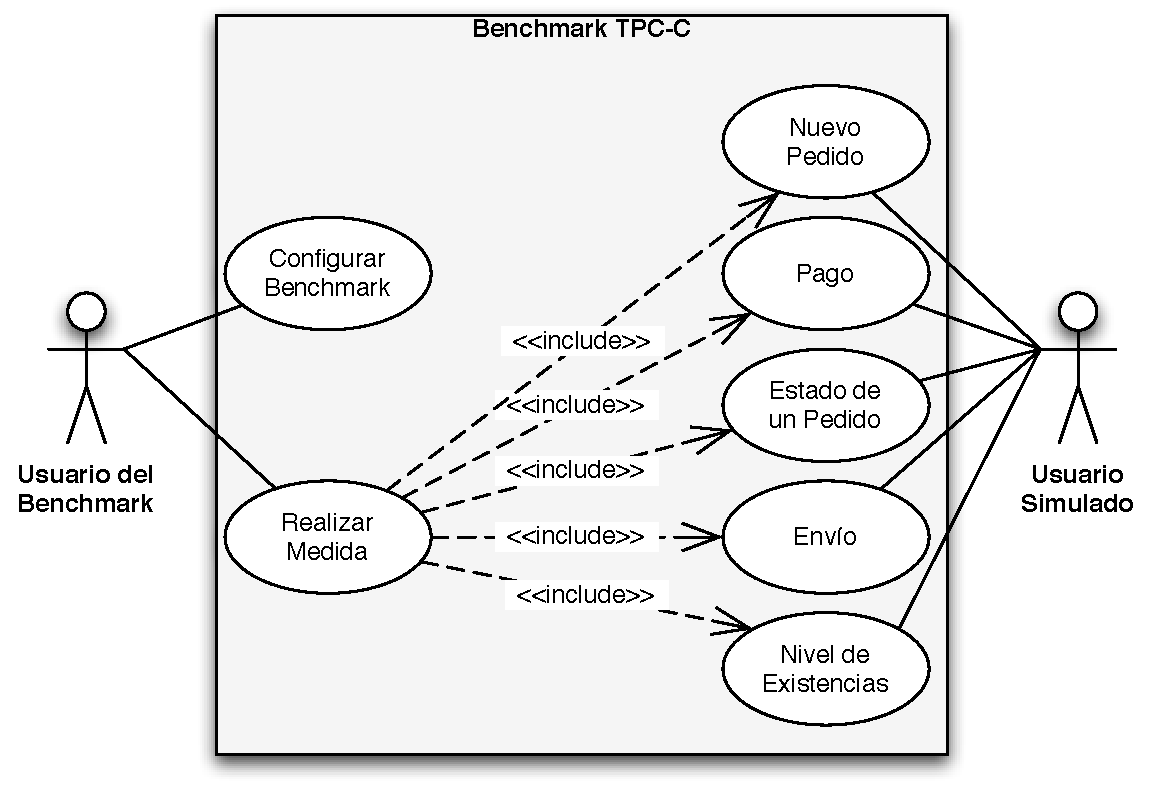
\includegraphics[width=\linewidth]{cap3/casosdeuso.pdf}
\caption{Casos de uso del benchmark TPC-C}
\label{fig:casosuso}
\end{center}
\end{figure}

\subsubsection{Configurar Benchmark}
\paragraph{Introducci�n}
A la hora de ejecutar el benchmark, existen unos par�metros importantes de los
que depende el resultado final y el modo de trabajo del benchmark. Es aqu� donde
se indica que necesita el benchmark para funcionar.
\paragraph{Actores}
El usuario del benchmark.
\paragraph{Pre condiciones}
Ninguna, ya que esto sucede lo primero de todo.
\paragraph{Post condiciones}
El benchmark se considera \textit{configurado} y se puede ejecutar con esta
configuraci�n.
\paragraph{Acciones}
\begin{enumerate}
\item El usuario del benchmark indica que quiere configurar los par�metros de
ejecuci�n del benchmark TPC-C.
\item El sistema le facilita un interfaz para realizar dicha configuraci�n.
\item El usuario introduce:
	\begin{itemize}
	\item El n�mero de terminales que van a simularse.
	\item Cu�ntas transacciones van a realizarse en total.
	\item El n�mero de almacenes a la hora de generar un poblado de datos.
	\end{itemize}
\item El sistema almacena dichos datos como una configuraci�n del benchmark.
\item El sistema queda listo para ejecutarse con esa nueva configuraci�n.
\end{enumerate}
\paragraph{Relaciones con otros casos de uso}
De manera directa ninguna, pero lo sucedido en este caso de uso es necesario
para que el resto de casos de uso funcionen.

\subsubsection{Realizar Medida}
\paragraph{Introducci�n}
Esta es la ejecuci�n del benchmark puramente, donde se realizan una serie de
tareas y se obtienen unos resultados en base a la m�trica de rendimiento que se
ha definido en el an�lisis. Este caso de uso depende de aquellos casos de uso
que simbolizan al usuario simulado y las tareas que realiza.
\paragraph{Actores}
El usuario del benchmark.
\paragraph{Pre condiciones}
El sistema tiene que estar \textit{configurado}, por lo que se debe disponer de
alguna configuraci�n antes de ejecutar el benchmark.
\paragraph{Post condiciones}
\begin{itemize}
\item Se obtiene una medici�n del rendimiento del sistema as� como otros datos
estad�sticos.
\item Se ha ejecutado el benchmark correctamente.
\end{itemize}
\paragraph{Acciones}
\begin{enumerate}
\item El usuario indica al sistema una configuraci�n del mismo y lo lanza para
obtener una medici�n de rendimiento.
\item El sistema crea una serie de tablas en un medio de almacenamiento y las
puebla (llena de datos) tal y como se indica en la secci�n de \textit{Poblado}
(Pag. \pageref{sec:poblado}).

Para ello utiliza el par�metro de configuraci�n referente al n�mero de
almacenes.
\item El sistema prepara el n�mero de terminales indicadas y con ese n�mero
prepara tambi�n el
n�mero de instancias del sistema de almacenamiento de datos que deben estar
preparadas para responder a la carga.
\item El sistema reparte el n�mero total de transacciones entre las terminales.
\item Cada terminal ejecuta las transacciones adecuadas para cumplir el
porcentaje de transacciones indicado en la secci�n de \textit{M�trica de
rendimiento} (Pag. \pageref{sec:metricarendimiento}).
	\begin{itemize}
	\item Nuevo pedido (\textit{$\ll include \gg$} Caso de uso de nuevo pedido).
	\item Pago (\textit{$\ll include \gg$} Caso de uso de Pago).
	\item Estado de un pedido (\textit{$\ll include \gg$} Caso de uso de Estado de un
	pedido).
	\item Env�o (\textit{$\ll include \gg$} Caso de uso de Env�o)
	\item Nivel de existencias (\textit{$\ll include \gg$} Caso de uso de Nivel de
	existencias).
	\end{itemize}
\item El sistema espera informaci�n por parte de los servidores encargados de
atender las peticiones de las terminales.
\item El sistema realiza una estad�stica y muestra la medida de rendimiento as�
como infamaci�n extra del n�mero de transacciones ejecutadas.
\end{enumerate}
\paragraph{Relaciones con otros casos de uso}
Para la correcta realizaci�n de este caso de uso se necesita de los siguientes
casos de uso: Nuevo Pedido, Pago, Estado de un pedido, Env�o y Nivel de
existencias.

\subsubsection{Nuevo Pedido}
\paragraph{Introducci�n}
Transacci�n de nuevo pedido, donde el sistema simula que la entrada de un pedido
adicional al negocio.
\paragraph{Actores}
El usuario simulado.
\paragraph{Pre condiciones}
\begin{itemize}
\item Es sistema est� en ejecuci�n.
\item El sistema de almacenamiento ha sido poblado con datos seg�n las reglas de
poblado (Pag. \ref{sec:poblado}).
\item Esta transacci�n se ejecuta en un servidor lanzado para atender a las
peticiones de una terminal simulada.
\end{itemize}
\paragraph{Post condiciones}
\begin{itemize}
\item Se ha insertado un nuevo pedido en el sistema
\item El sistema de benchmark sigue funcionando.
\item El sistema de almacenamiento contiene datos correctos y no corruptos.
\end{itemize}
\paragraph{Acciones}
\begin{enumerate}
\item El usuario simulado ha decidido que quiere realizar una transacci�n de
nuevo pedido.
\item El usuario simulado provee de los datos necesarios para dicha transacci�n
a la terminal (Todos los detalles en \textit{Nuevo Pedido, datos de entrada},
Pag. \pageref{sec:nuevopedido-datosdeentrada}).
	\begin{enumerate}
	\item El n�mero de almac�n local (W\_ID). 
	\item El n�mero de la zona (D\_ID). 
	\item El n�mero de l�neas de pedido (O\_OL\_CNT). 
	\item Para cada l�nea de pedido: 
		\begin{enumerate}
		\item Un n�mero de producto (OL\_I\_ID).
		\item Almac�n que provee el producto (OL\_SUPPLY\_W\_ID).
		\item Una cantidad de producto (OL\_QUANTITY).
		\item Una fecha para el pedido (O\_ENTRY\_D).
		\end{enumerate}
	\end{enumerate}
\item La terminal encarga el siguiente trabajo al servidor que se le ha
asignado (Todos los detalles en \textit{Nuevo Pedido, perfil de la transacci�n},
Pag. \pageref{sec:nuevopedido-perfil}).
	\begin{enumerate}
	\item Obtener los datos del almac�n W\_ID.
	\item Obtener los datos de la zona D\_W\_ID,D\_ID e incrementar
	O\_NEXT\_O\_ID.
	\item Obtener el cliente C\_W\_ID, C\_D\_ID, C\_ID y obtener sus datos.
	\item Crear una entrada en pedido y en nuevo pedido con la misma clave.
	\item Para cada l�nea de pedido:
		\begin{enumerate}
		\item Buscamos el producto.
		\item Actualizamos las existencias del producto en el almac�n.
		\item Calculamos el precio de esa l�nea
		\item Insertamos una tupla en l�neas de pedido con estos datos.
		\end{enumerate}
	\end{enumerate}	
\item La transacci�n se da por finalizada.
\end{enumerate}
\paragraph{Relaciones con otros casos de uso}
Es utilizado por el caso de uso: realizar medida.

\subsubsection{Pago}
\paragraph{Introducci�n}
Transacci�n de pago, donde se simula que un cliente paga una cantidad de dinero
para cubrir su deuda con la empresa.
\paragraph{Actores}
El usuario simulado.
\paragraph{Pre condiciones}
\begin{itemize}
\item Es sistema est� en ejecuci�n.
\item El sistema de almacenamiento ha sido poblado con datos seg�n las reglas
de poblado (Pag. \pageref{sec:poblado}).
\item Esta transacci�n se ejecuta en un servidor lanzado para atender a
las peticiones de una terminal simulada.
\end{itemize}

\paragraph{Post condiciones}
\begin{itemize}
\item Se ha anotado el pago del cliente.
\item El sistema de benchmark sigue funcionando.
\item El sistema de almacenamiento contiene datos correctos y no corruptos.
\end{itemize}

\paragraph{Acciones}
\begin{enumerate}
\item El usuario simulado ha decidido que quiere realizar una transacci�n de
pago.
\item El usuario simulado provee de los datos necesarios para dicha transacci�n
a la terminal (Todos los detalles en \textit{Pago, datos de entrada}, Pag
\pageref{sec:pago-datosdeentrada}).
	\begin{enumerate}
	\item El n�mero de almac�n (W\_ID).
	\item El n�mero de la zona (D\_ID).
	\item Los datos de un cliente: a veces por su identificador  (C\_W\_ID,
	C\_D\_ID, C\_ID), y a veces por su apellido (C\_LAST).
	\item La cantidad a pagar (H\_AMOUNT).
	\item La fecha del pago (H\_DATE).
	\end{enumerate}
\item La terminal encarga el siguiente trabajo al servidor que se le ha asignado
(Todos los detalles en \textit{Pago, perfil de la transacci�n}, Pag.
\pageref{sec:pago-perfil}).
	\begin{enumerate}
	\item Obtener los datos del almac�n (W\_ID) e incrementar su balance
	econ�mico en H\_AMOUNT.
	\item Obtener los datos de la zona (D\_W\_ID, D\_ID) e incrementar su
	balance econ�mico en H\_AMOUNT.
	\item Obtener los datos del cliente y:
		\begin{enumerate}
		\item Incrementar su balance anual en H\_AMOUNT.
		\item Disminuir el balance actual en H\_AMOUNT.
		\item Incrementar en uno el n�mero de pagos.
		\item Dependiendo del campo C\_CREDIT actualizar el campo
		C\_DATA.
		\end{enumerate}
	\item Preparar una entrada en el hist�rico con su campo H\_DATA.
	\item A�adir dicha entrada al hist�rico.
	\end{enumerate}
\end{enumerate}
\paragraph{Relaciones con otros casos de uso}
Es utilizado por el caso de uso: realizar medida.

\subsubsection{Estado de un pedido}
\paragraph{Introducci�n}
Transacci�n de consulta de estado de un pedido; el sistema simula consultar el
estado del �ltimo pedido realizado por el cliente.
\paragraph{Actores}
El usuario simulado.
\paragraph{Pre condiciones}
\begin{itemize}
\item Es sistema est� en ejecuci�n.
\item El sistema de almacenamiento ha sido poblado con datos seg�n las reglas
de poblado (Pag. \pageref{sec:poblado}).
\item Esta transacci�n se ejecuta en un servidor lanzado para atender a las 
peticiones de una terminal simulada.
\end{itemize}
\paragraph{Post condiciones}
\begin{itemize}
\item Se ha informado al cliente del estado de su �ltimo pedido.
\item El sistema de benchmark sigue funcionando.
\item El sistema de almacenamiento contiene datos correctos y no corruptos.
\end{itemize}

\paragraph{Acciones}
\begin{enumerate}
\item El usuario simulado ha decidido que quiere realizar una transacci�n de
consulta de estado de un pedido.
\item El usuario simulado provee de los datos necesarios para dicha transacci�n
a la terminal (Todos los detalles en \textit{Estado de pedido, datos de entrada},
Pag. \pageref{sec:estado-datosdeentrada}).
	\begin{enumerate}
	\item El n�mero de almac�n (W\_ID).
	\item El n�mero de la zona (D\_ID).
	\item Los datos de un cliente: a veces por su identificador  (C\_W\_ID,
	C\_D\_ID, C\_ID), y a veces por su apellido (C\_LAST).
	\end{enumerate}
\item La terminal encarga el siguiente trabajo al servidor que se le ha asignado
(Todos los detalles en \textit{Estado de pedido, perfil de la transacci�n}, Pag.
\pageref{sec:estado-perfil}).
	\begin{enumerate}
	\item Se obtienen los datos del cliente.
	\item Se obtiene el pedido del cliente con mayor O\_ID.
	\item Se obtienen todas las l�neas de dicho pedido.
	\end{enumerate}
\end{enumerate}
\paragraph{Relaciones con otros casos de uso}
Es utilizado por el caso de uso: realizar medida.

\subsubsection{Env�o}
\paragraph{Introducci�n}
Transacci�n de env�o, donde el sistema elige un pedido que no est� enviado,
selecciona uno de cada zona por cada almac�n, y lo tramita como enviado.

\paragraph{Actores}
El usuario simulado.

\paragraph{Pre condiciones}
\begin{itemize}
\item Es sistema est� en ejecuci�n.
\item El sistema de almacenamiento ha sido poblado con datos seg�n las reglas
de poblado (Pag. \pageref{sec:poblado}).
\item Esta transacci�n se ejecuta en un servidor lanzado para atender a
las peticiones de una terminal simulada.
\end{itemize}

\paragraph{Post condiciones}
\begin{itemize}
\item Se ha marcado el pedido como enviado.
\item El sistema de benchmark sigue funcionando.
\item El sistema de almacenamiento contiene datos correctos y no corruptos.
\end{itemize}

\paragraph{Acciones}
\begin{enumerate}
\item El usuario simulado ha decidido que quiere realizar una transacci�n de
env�o de pedidos.
\item El usuario simulado provee de los datos necesarios para dicha transacci�n
a la terminal (Todos los detalles en \textit{Env�o, datos de entrada}, Pag.
\pageref{sec:envio-datosdeentrada}).
	\begin{enumerate}
	\item El n�mero de almac�n (W\_ID).
	\item El n�mero de la empresa de transportes (O\_CARRIER\_ID).
	\item La fecha de env�o (OL\_DELIVERY\_D).
	\end{enumerate}
\item La terminal encarga el siguiente trabajo al servidor que se le ha asignado
(Todos los detalles en \textit{Env�o, perfil de la transacci�n}, Pag.
\pageref{sec:envio-perfil}). Para cada una de las zonas del almac�n escogido:
	\begin{enumerate}
	\item Se selecciona el nuevo pedido m�s viejo, es decir el NO\_O\_ID m�s
	peque�o, y se borra.
	\item Se selecciona el pedido correspondiente al nuevo pedido borrado y
	se actualiza la empresa de transportes (O\_CARRIER\_ID).
	\item Para todas las l�neas de pedido, calculamos el coste total y
	actualizamos en cada l�nea la fecha de env�o.
	\item Al balance actual del cliente se le suma el total de las l�neas de
	pedido y se incrementa el n�mero de pedidos enviados a ese cliente.
	\end{enumerate}
\end{enumerate}
\paragraph{Relaciones con otros casos de uso}
Es utilizado por el caso de uso: realizar medida.

\subsubsection{Nivel de existencias}
\paragraph{Introducci�n}
Transacci�n de consulta de nivel de existencias, donde se revisan las �ltimas
l�neas de pedido de los �ltimos 20 pedidos en una zona y de esos productos se
comprueban las existencias por si hace falta encargar m�s.

\paragraph{Actores}
El usuario simulado.

\paragraph{Pre condiciones}
\begin{itemize}
\item Es sistema est� en ejecuci�n.
\item El sistema de almacenamiento ha sido poblado con datos seg�n las reglas
de poblado (Pag. \pageref{sec:poblado}).
\item Esta transacci�n se ejecuta en un servidor lanzado para atender a
las peticiones de una terminal simulada.
\end{itemize}

\paragraph{Post condiciones}
\begin{itemize}
\item Se ha comprobado sin problemas las existencias de los productos incluidos
en los �ltimos 20 pedidos de una zona.
\item El sistema de benchmark sigue funcionando.
\item El sistema de almacenamiento contiene datos correctos y no corruptos.
\end{itemize}

\paragraph{Acciones}
\begin{enumerate}
\item El usuario simulado ha decidido que quiere realizar una transacci�n de
comprobar el nivel de existencias.
\item El usuario simulado provee de los datos necesarios para dicha transacci�n
a la terminal (Todos los detalles en \textit{Nivel de existencias, datos de
entrada}, Pag. \pageref{sec:nivel-datosdeentrada}).
	\begin{enumerate}
	\item Un almac�n (W\_ID).
	\item Una zona dentro de ese almac�n (D\_ID).
	\item Un l�mite m�nimo de existencias.
	\end{enumerate}
\item La terminal encarga el siguiente trabajo al servidor que se le ha asignado
(Todos los detalles en \textit{Nivel de existencias, perfil de la transacci�n}, Pag.
\pageref{sec:nivel-perfil}).
	\begin{enumerate}
	\item Obtenemos los datos de la zona, incluyendo el pr�ximo n�mero de
	pedido.
	\item Obtenemos todas las l�neas de pedido correspondientes a los
	�ltimos 20 pedidos de esa zona.
	\item Para cada producto en la l�nea de pedido, comprobamos que el stock
	del almac�n no est� por debajo del l�mite indicado.
	\end{enumerate}
\end{enumerate}


\paragraph{Relaciones con otros casos de uso}
Es utilizado por el caso de uso: realizar medida.

\subsection{Diagramas de secuencia}
Por �ltimo, dentro de los casos de uso y para intentar sacar una peque�a lista de clases o subsistemas de
an�lisis, as� como intentar ver las partes en las que se divide la organizaci�n
del benchmark TPC-C con las especificaciones que hemos indicado; se incluyen los
diagramas de secuencia para los casos de uso m�s significativos.

\subsubsection{Configurar Benchmark}
Figura \ref{fig:sec-conf}.
\begin{figure}[htb]
\begin{center}
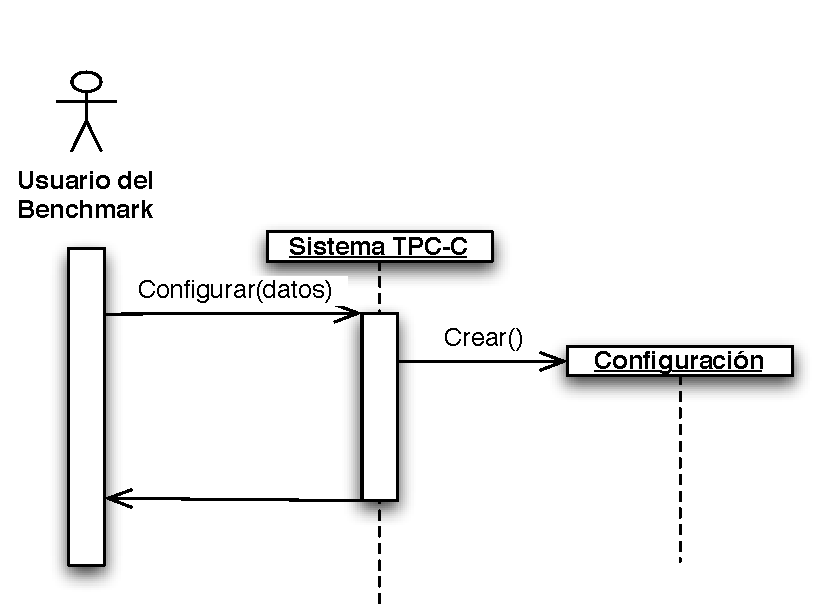
\includegraphics[width=8cm]{cap3/secuencia-configurar.pdf}
\end{center}
\caption{Diagrama de secuencia del caso de uso \textit{Configurar Benchmark}}
\label{fig:sec-conf}
\end{figure}
\afterpage{\clearpage}

\subsubsection{Realizar Medida}
Figura \ref{fig:sec-real}.
\begin{figure}[htb]
\begin{center}
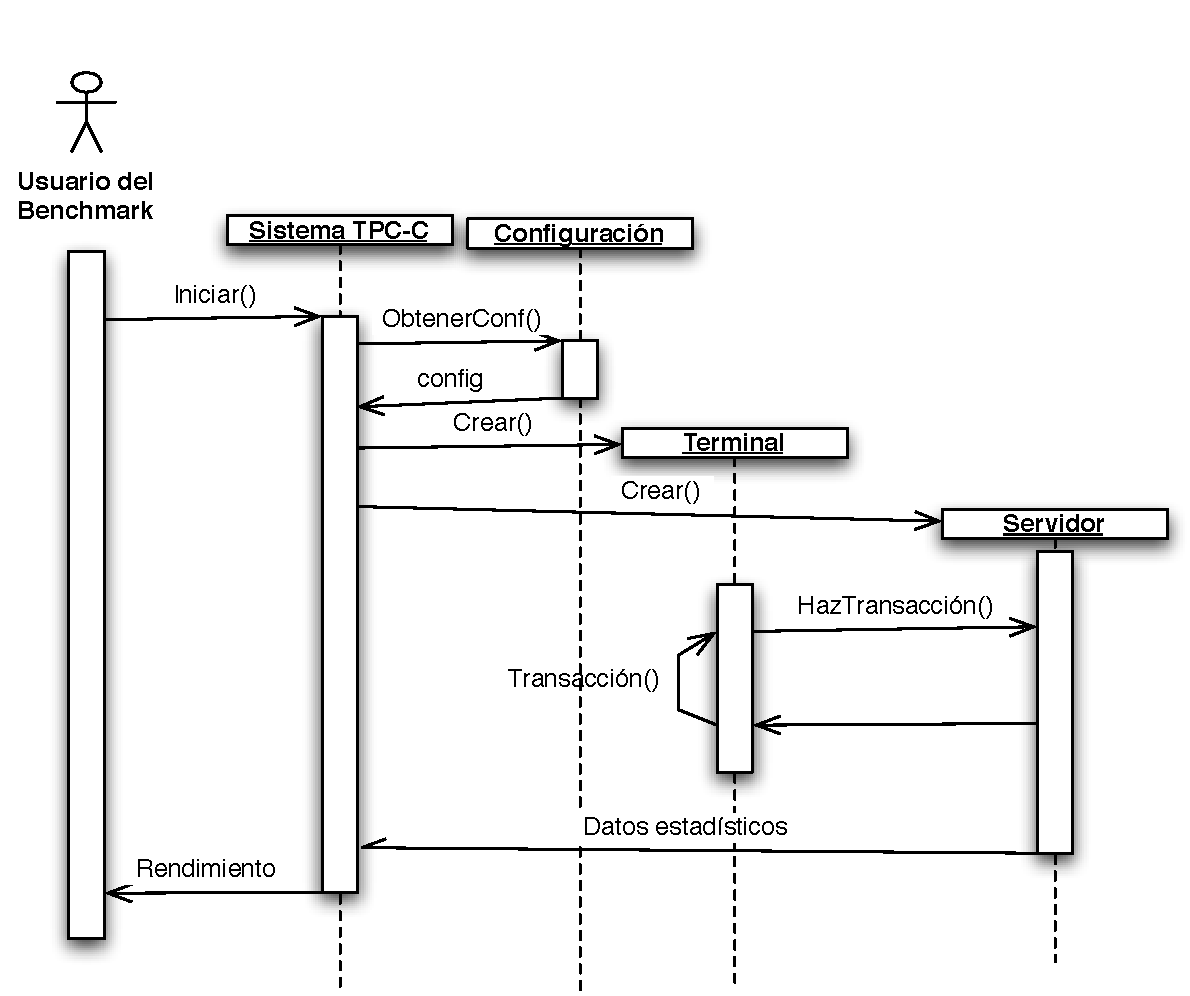
\includegraphics[width=13.5cm]{cap3/secuencia-ejecutar.pdf}
\end{center}
\caption{Diagrama de secuencia del caso de uso \textit{Realizar Medida}}
\label{fig:sec-real}
\end{figure}

\subsubsection{Nuevo Pedido}
Figura \ref{fig:sec-np}.
\begin{figure}[htb]
\begin{center}
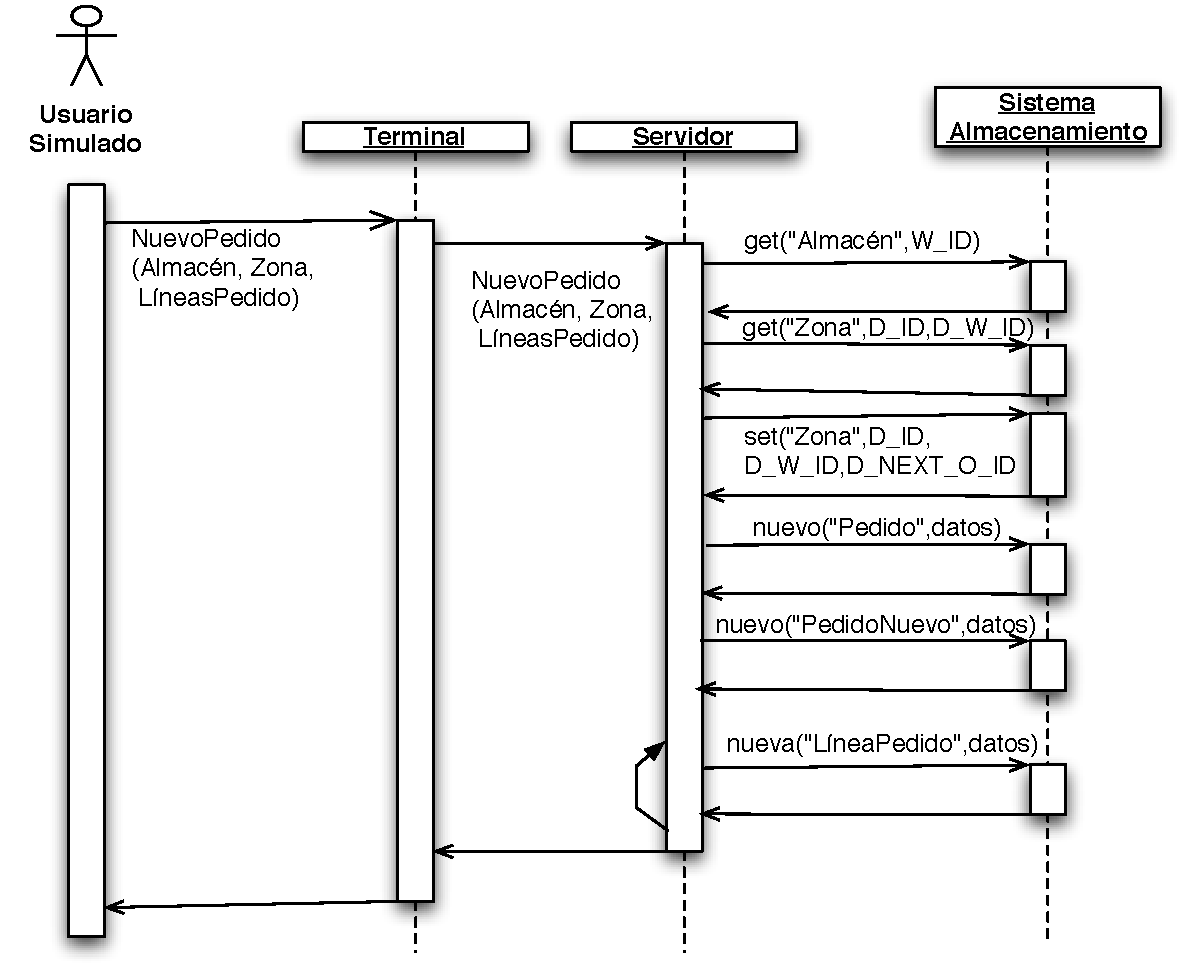
\includegraphics[width=13.5cm]{cap3/secuencia-nuevopedido.pdf}
\end{center}
\caption{Diagrama de secuencia del caso de uso \textit{Nuevo Pedido}}
\label{fig:sec-np}
\end{figure}

\subsection{Diagrama de clases de an�lisis}
De estos diagramas de secuencia, ya que se han expuesto algunas posibles clases,
podemos derivar las siguientes clases de an�lisis.
\begin{itemize}
\item \textit{Clase Terminal}: Dado que el usuario simulado, al fin y al cabo
es simulado, los datos necesarios para cada transacci�n los \textit{generar�}
esta clase.
\item \textit{Clase Servidor}: Es la encargada de realizar las transacciones;
tiene una lista de los almacenes disponibles, y los utiliza como referencia para
acceder a los datos. Realiza la l�gica de negocio.
\item \textit{Clase Sistema Almacenamiento}: Maneja las estructuras de datos
para acceder, a�adir, borrar y modificar registros de datos. Esta clase es usada
por los m�ltiples servidores de manera concurrente.
\item \textit{Clase IdAlmacenamiento}: Para completar a la clase servidor, y dado que en
alg�n lugar se tienen que guardar las referencias a los diferentes sistemas de
almacenamiento, que m�s tarde se enviaran al sistema de almacenamiento para que
opere con ellos, se ha creado esta clase.
\end{itemize}

El diagrama de clases de an�lisis se encuentra en la figura
\ref{fig:analisis-clases}.

\begin{figure}
\begin{center}
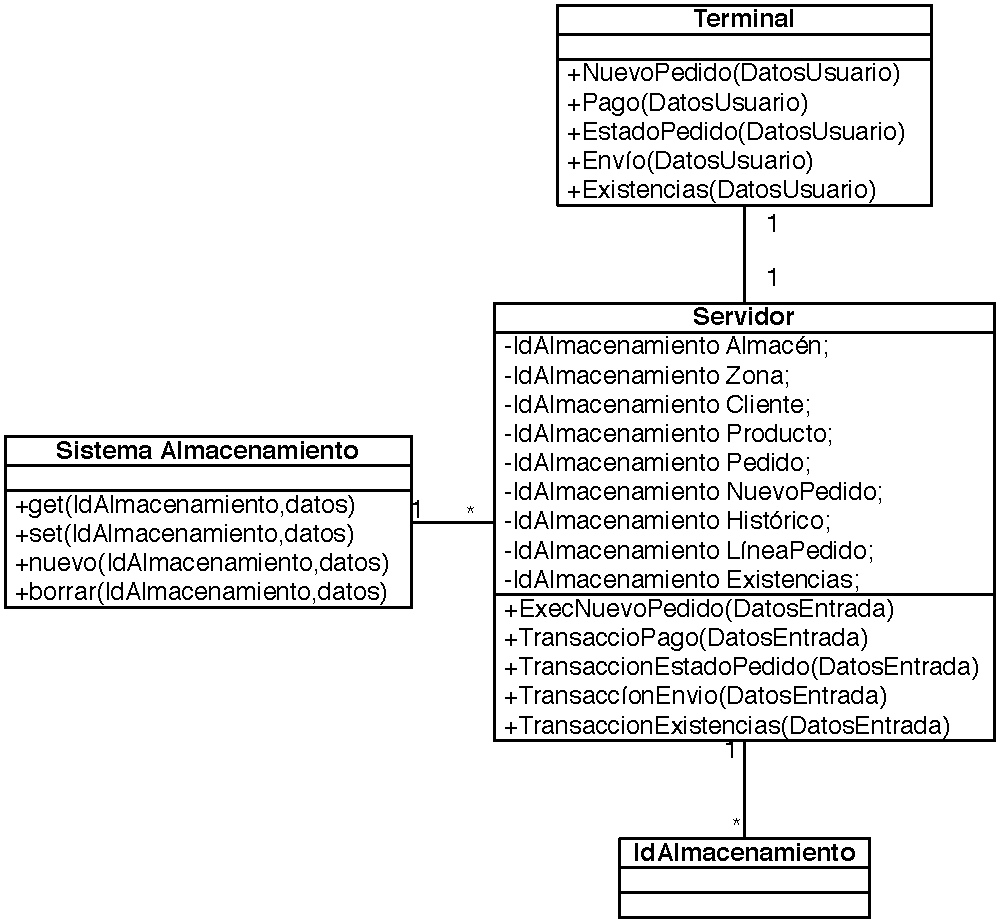
\includegraphics[width=\textwidth]{cap3/analisis-clases.pdf}
\end{center}
\caption{Diagrama de clases de an�lisis}
\label{fig:analisis-clases}
\end{figure}

% Dise�o
\chapter{Dise�o e implementaci�n}
En las especificaciones originales del benchmark TPC-C, existen reglas y
par�metros para realizar un an�lisis de rendimiento completo: desde la
herramienta a implementar, hasta plantillas para los documentos que hay que
presentar as� como una explicaci�n detallada de los datos a obtener.

En este caso lo que se va a dise�ar e implementar es la herramienta que permite
obtener un resultado num�rico del rendimiento de un sistema con su simple
ejecuci�n con una configuraci�n concreta.

\section{Dise�o de la arquitectura}
Para explicar el dise�o descendente que se ha realizado, se empezar� por el
diagrama de arquitectura, que dar� paso a los diferentes subsistemas de la
aplicaci�n. Ya que la aplicaci�n de primeras tiene dos partes diferenciadas:
subsistema de medida de rendimiento y subsistema de almacenamiento de datos, el
trabajo aplicado para dividir lo mejor posible en m�dulos el programa ha sido
importante, ya que si no, la cantidad de c�digo acumulada en un solo fichero
hubiera hecho dif�cil la b�squeda y soluci�n de problemas, as� como casi
imposible la adaptaci�n a peque�os cambios o actualizaciones.

\subsection{Dise�o de los subsistemas}
Empezaremos con una divisi�n funcional de los componentes del sistema agrupados
en subsistemas. El sistema principal que implementa el benchmark se divide en 3
subsistemas (Fig. \ref{fig:subsistemas}).

\begin{figure}
\begin{center}
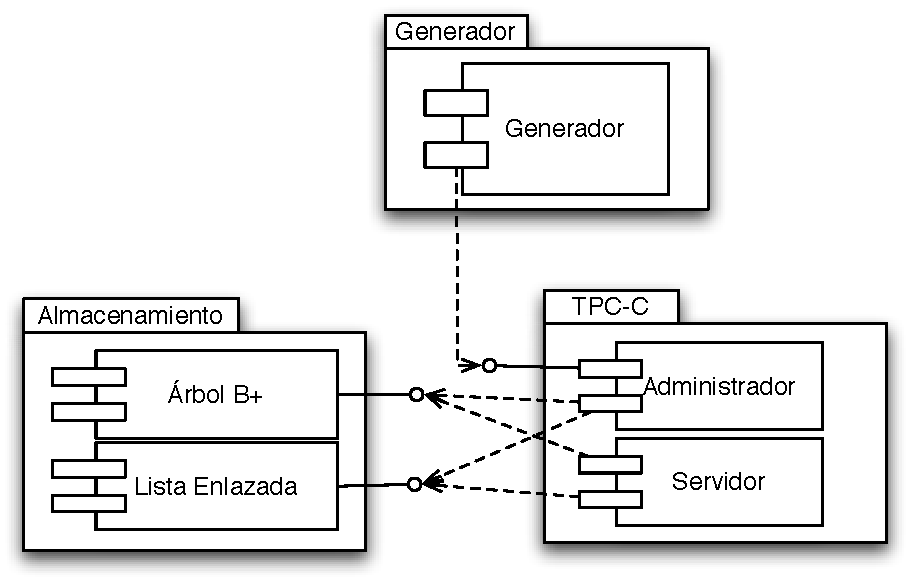
\includegraphics[width=10cm]{cap4/subsistemas.pdf}
\end{center}
\caption{Diferentes subsistemas del benchmark TPC-C}
\label{fig:subsistemas}
\end{figure}

\begin{itemize}
\item Subsistema generador: Se encarga de generar los datos de \textit{poblado}
como los datos de los usuarios simulados que al final acaban siendo los datos
que las \textit{terminales} env�an a los servidores para que realicen una
transacci�n.
\item Subsistema TPC-C: es el programa principal del benchmark, que se divide en
2 componentes:
	\begin{itemize}
	\item Administrador: es el encargado de cuidar y preparar el sistema
	para que los servidores comiencen su trabajo. Realiza las siguientes
	tareas cortas:
		\begin{itemize}
		\item Inicializa el subsistema de almacenamiento.
		\item Carga el \textit{poblado} generado anteriormente en el
		subsistema de almacenamiento.
		\item Lanza los servidores.
		\item Espera sus estad�sticas y las da un formato final.
		\end{itemize}
	\item Servidor: se encarga de realizar las transacciones que tiene
	indicadas en los datos que las \textit{terminales} le han encargado.
	Trabaja de manera conjunta con el subsistema de almacenamiento: el
	servidor se encarga de la l�gica del negocio, y el almacenamiento de
	guardar y recuperar los datos.
	\end{itemize}
\item Subsistema de almacenamiento: Se encarga de almacenar datos de manera
gen�rica y de proporcionar un m�todo r�pido de acceso y modificaci�n de los
mismos. Dado que no siempre las necesidades son las mismas, se emplean 2
componentes para prestar este servicio:
	\begin{itemize}
	\item �rbol B+: proporciona un m�todo de almacenamiento indexado, donde
	se permite: buscar, insertar, eliminar y modificar; siendo la operaci�n
	m�s r�pida la de buscar.
	\item Lista Enlazada: debido a que hay tablas que no tienen clave, este
	sistema de almacenamiento permite de una manera sencilla almacenar estos
	datos sin campos clave. Solo permite 2 operaciones: a�adir y borrar.
	\end{itemize}
En ambos componentes existe una \textit{sincronizaci�n} para que m�ltiples
procesos o hilos de ejecuci�n puedan acceder a los datos sin interferir entre
si.
\end{itemize}

\subsection{Dise�o detallado de la arquitectura}
Existen varios subsistemas y no todos ellos se ejecutan a la vez, ni en el mismo
proceso, por lo que hace falta un diagrama que explique claramente c�mo es el
funcionamiento habitual del benchmark antes de explicar en detalle los
fundamentos y la composici�n de cada subsistema.

\begin{figure}
\begin{center}
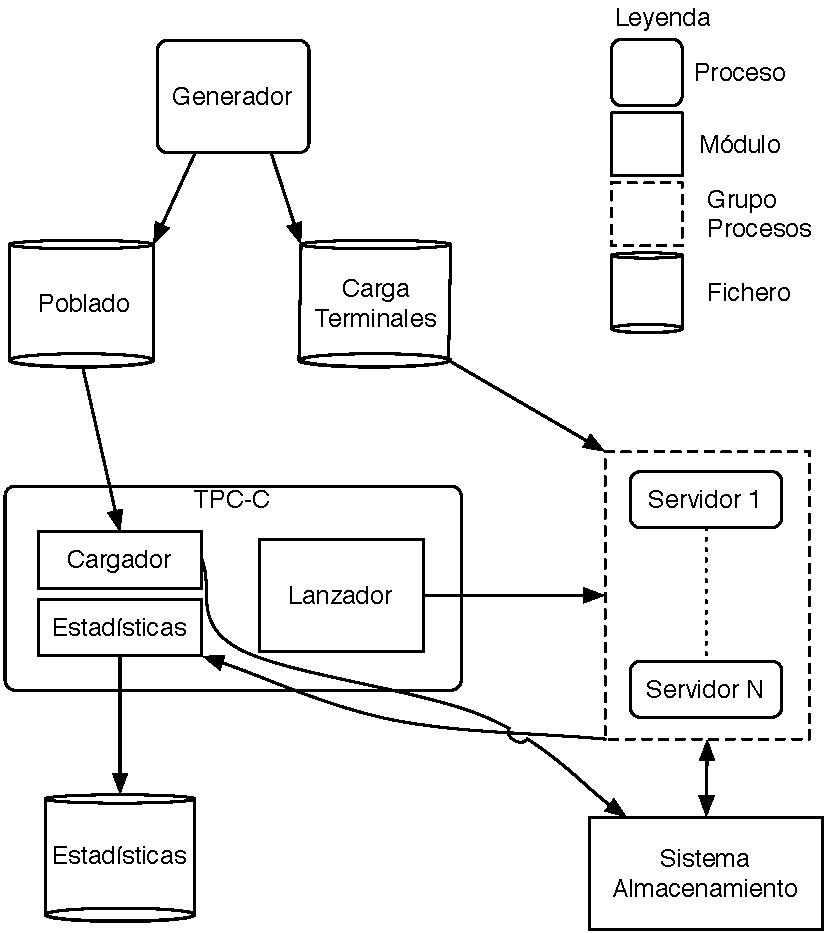
\includegraphics[width=10cm]{cap4/arquitectura.pdf}
\end{center}
\caption{Arquitectura del sistema TPC-C}
\label{fig:arquitectura}
\end{figure}

En la figura \ref{fig:arquitectura}, se puede observar de manera menos est�ndar
(sin usar UML) c�mo se distribuye todo el sistema TPC-C en diferentes sistemas y
procesos, por lo que se va detallar el funcionamiento de los mismos.


\begin{enumerate}
\item \textbf{Proceso Generador:} es el primero que se ejecuta para producir un
\textit{experimento} que consiste en:
	\begin{itemize}
	\item Unos datos de \textit{poblado}, que servir�n como datos iniciales
	a la hora de que los servidores comiencen a funcionar.
	\item Simula a los usuarios de las terminales, y con ello genera unos
	datos que son los que recibir�n los servidores para realizar las
	transacciones. Es lo que llamaremos \textit{carga} de trabajo generada
	por las terminales.
	\end{itemize}
El proceso generador necesita adem�s los par�metros de funcionamiento:
	\begin{itemize}
	\item La cantidad de \textit{almacenes} para poblar la base de datos.
	Recordemos que el almac�n es la unidad de generaci�n de carga
	inicial, cada almac�n contiene 10 zonas, y cada zona sus clientes
	pedidos y entradas en el hist�rico; por lo que al multiplicar el n�mero
	de almacenes se multiplican tambi�n estos datos.
	\item La cantidad de \textit{servidores} que simult�neamente van a
	atender peticiones de las terminales. Con este par�metro se generar�n
	diferentes ficheros de \textit{carga}
	\item Pero para contabilizar esta carga hace falta indicar tambi�n el
	\textit{n�mero de transacciones} que se van a ejecutar en total; seg�n
	este n�mero, se repartir�n esas transacciones entre los diferentes
	servidores.
	\end{itemize}
Por lo que al finalizar la ejecuci�n del proceso generador obtenemos los datos
de un \textit{experimento} en \textbf{ficheros}, que son:
	\begin{itemize}
	\item Datos de poblado del sistema de almacenamiento.
	\item N�mero de servidores.
	\item Carga para dichos servidores.
	\end{itemize}
\item \textbf{Proceso TPC-C:} Es el encargado de realizar la medici�n del
rendimiento, para ello preparar� los datos necesarios para que el sistema pueda
trabajar.
	\begin{enumerate}
	\item Lo primero es ejecutar un \textit{cargador}, que inicializa los
	sistemas de almacenamiento y los puebla con los datos de poblado. Es una
	operaci�n repetitiva y no se tiene en cuenta a la hora de medir el
	rendimiento.
	\item Luego se prepara la sincronizaci�n de los procesos servidores y se
	\textit{lanzan}, dichos procesos servidores, son unidades de ejecuci�n
	independientes que seg�n el modelo de paralelizaci�n pueden ser hilos de
	ejecuci�n o procesos.
	\item Por �ltimo, espera a que terminen los servidores, y mediante
	\textbf{memoria compartida} recoge los datos estad�sticos de cada
	servidor y escribe un fichero con un resumen y una medida de
	rendimiento.
	\end{enumerate}
En este proceso se ejecuta el \textit{subsistema de almacenamiento}, este
sistema es el mismo entre los procesos TPC-C y servidores gracias a que est�
situado en \textbf{memoria compartida}, por lo que los datos almacenados en la
fase de carga son los mismos que se utilizar�n por los servidores.
\item \textbf{Proceso servidor:} Pueden existir m�ltiples procesos servidores,
pero se explicar� el funcionamiento de uno en concreto. Cuando se lanza un
proceso servidor, este realiza un trabajo c�clico consistente en procesar
transacciones; este es el orden de operaciones:
	\begin{enumerate}
	\item Obtiene una transacci�n junto con sus datos del fichero de carga.
	\item La identifica y la realiza.
	\item Anota la transacci�n realizada en un �rea de \textbf{memoria
	compartida}.
	\end{enumerate}
Si bien este proceso parece sencillo, es el que m�s trabajo necesita para
realizarse ya que cada transacci�n lleva impl�cita una carga de trabajo. Tambi�n
es aqu� donde se explotan todas las caracter�sticas de multiproceso del sistema
de almacenamiento mediante un sistema \textit{lector-escritor} que se explicar�
m�s adelante. Este sistema permite una ordenaci�n de los accesos de tal manera
que para una tabla, s�lo un proceso pueda estar modific�ndola, pero cuando no se
est� modificando, m�ltiples procesos puedan estar accediendo a sus datos.
\end{enumerate}

\subsection{Tecnolog�as de la implementaci�n}
Una vez definida la arquitectura, hay que fijar que tecnolog�as se utilizar�n;
es verdad que definiendo la arquitectura ya se han dicho bastantes de estas
tecnolog�as, pero vamos a listar e introducir cada una de ellas.

\subsubsection{�rboles B+}\label{sec:arbolbmasbasico}
Los �rboles B y los �rboles B+ \cite{marques01} son casos especiales de �rboles de b�squeda. Un
�rbol de b�squeda es un tipo de �rbol que sirve para guiar la localizaci�n de un
registro, dado el valor de uno de sus campos. Los �ndices multinivel 
pueden considerarse como variaciones de los �rboles de
b�squeda. Cada bloque o nodo del �ndice multinivel puede tener hasta $p$ valores
del campo de indexaci�n y $p$  punteros. Los valores del campo de indexaci�n de cada
nodo gu�an al siguiente nodo (que se encuentra en otro nivel), hasta llegar al
bloque del fichero de datos que contiene el registro deseado. Al seguir un
puntero, se va restringiendo la b�squeda en cada nivel a un sub�rbol del �rbol
de b�squeda, y se ignoran todos los nodos que no est�n en dicho sub�rbol.

Los �rboles de b�squeda difieren un poco de los �ndices multinivel. Un �rbol de
b�squeda de orden $p$ es un �rbol tal que cada nodo contiene como mucho $p-1$  valores
del campo de indexaci�n y $p$  punteros, colocados de la siguiente manera:
\begin{equation}
(P_1,K_1,P_2,K_2,...,P_{q-1},K_{q-1},P_q)
\end{equation}

Donde:
\begin{itemize}
\item $q\leq p$
\item $P_i$ es un puntero a un nodo hijo.
\item $K_i$ es un valor de b�squeda o valor clave.
\end{itemize}

Adem�s se cumple que:
\begin{enumerate}
\item Todos los valores de b�squeda son �nicos.
\item Dentro de cada nodo se cumple: $K_1<K_2<...K_{q-1}$
\item Para todos los valores de $X$ del sub�rbol al que nos lleva el puntero
$P_i$, se tiene: 
	\begin{itemize}
	\item $K_{i-1}<X<K_i$ para $1<i<q$
	\item $X<K_i$ para $i=1$
	\item $K_{i-1}<X$ para $i=q$
	\end{itemize}
\end{enumerate}

Al buscar un valor $X$, se sigue el puntero $P_i$ apropiado de acuerdo con las
3 restricciones del punto 3.  Para insertar valores de b�squeda en el �rbol y
eliminarlos, sin violar las restricciones anteriores, se utilizan algoritmos que
no garantizan que el �rbol de b�squeda est� equilibrado (que todas las hojas
est�n al mismo nivel). Es importante mantener equilibrados los �rboles de
b�squeda porque esto garantiza que no habr� nodos en niveles muy profundos que
requieran muchos accesos a bloques durante una b�squeda. Adem�s, las
eliminaciones de registros pueden hacer que queden nodos casi vac�os, con lo que
hay un desperdicio de espacio importante que tambi�n provoca un aumento en el
n�mero de niveles.

El �rbol B es un �rbol de b�squeda, con algunas restricciones adicionales, que
resuelve hasta cierto punto los dos problemas anteriores. Estas restricciones
adicionales garantizan que el �rbol siempre estar� equilibrado y que el espacio
desperdiciado por la eliminaci�n, si lo hay, nunca ser� excesivo. Los algoritmos
para insertar y eliminar se hacen m�s complejos para poder mantener estas
restricciones. No obstante, la mayor parte de las inserciones y eliminaciones
son procesos simples, se complican s�lo en circunstancias especiales: cuando se
intenta insertar en un nodo que est� lleno o cuando se intenta borrar en un nodo
que est� ocupado hasta la mitad.

\paragraph{�rbol B}
Un �rbol B de orden $p$, se define de la siguiente manera:
\begin{enumerate}
\item La estructura de cada nodo tiene la siguiente forma:
\begin{equation}
(P_1,(K_1,Pr_1),P_2,(K_2,Pr_2),P_3,(K_3,Pr_3),...P_{q-1},(K_{q-1},Pr_{q-1}),P_q)
\end{equation}
Donde:
	\begin{itemize}
	\item $q\leq p$
	\item $P_i$ es un puntero a un nodo hijo.
	\item $Pr_i$ es un puntero al nodo de datos cuya clave es $K_i$
	\end{itemize}
\item Dentro de cada nodo se cumple: $K_1<K_2<...K_{q-1}$
\item Para todos los valores de $X$ del sub�rbol al que nos lleva el puntero
$P_i$, se tiene: 
	\begin{itemize}
	\item $K_{i-1}<X<K_i$ para $1<i<q$
	\item $X<K_i$ para $i=1$
	\item $K_{i-1}<X$ para $i=q$
	\end{itemize}
\item Cada nodo tiene como mucho $p$ punteros a otros nodos del �rbol.
\item Cada nodo excepto el ra�z (el primero) y las hojas (los �ltimos), tiene al
menos $p/2$ punteros a nodos del �rbol. El nodo ra�z tiene como m�nimo 2
punteros a nodos del �rbol, excepto si es el �nico nodo.
\item Un nodo con $q$ punteros a nodos y $q\leq p$, tiene $q-1$ campos de
indexaci�n o campos clave.
\item Todos los nodos hoja est�n al mismo nivel. Los nodos hoja tienen la misma
estructura que los nodos internos, pero los punteros a nodos del �rbol son
nulos.
\end{enumerate}

Como se puede observar, en los �rboles B todos los valores del campo de
indexaci�n aparecen alguna vez en alg�n nivel del �rbol, junto con un puntero al
fichero de datos.

\paragraph{�rbol B+}
En un �rbol B+ los punteros a datos se almacenan s�lo en los nodos hoja del
�rbol, por lo cual, la estructura de los nodos hoja difiere de la de los nodos
internos. Los nodos hoja tienen una entrada por cada valor del campo de
indexaci�n, junto con un puntero al registro del fichero de datos. Estos nodos
est�n enlazados para ofrecer un acceso ordenado a los registros a trav�s del
campo de indexaci�n. Los nodos hoja de un �rbol B+ son similares al primer nivel
(nivel base) de un �ndice. Los nodos internos del �rbol B+ corresponden a los
dem�s niveles del �ndice. Algunos valores del campo de indexaci�n se repiten en
los nodos internos del �rbol B+ con el fin de guiar la b�squeda.

En un �rbol B+ de orden $p$, la estructura de los nodos \textit{internos} es la
siguiente:
\begin{enumerate}
\item Todo nodo interno es de la forma: 
\begin{equation}
(P_1,K_1,P_2,K_2,P_3,K_3,...P_{q-1},K_{q-1},P_q)
\end{equation}
Donde:
	\begin{itemize}
	\item $q\leq p$
	\item Cada $P_i$ es un puntero a un nodo interno u hoja del �rbol.
	\end{itemize}
\item Dentro de cada nodo interno se cumple: $K_1<K_2<...K_{q-1}$
\item Para todos los valores de $X$ del sub�rbol al que nos lleva el puntero
$P_i$, se tiene: 
	\begin{itemize}
	\item $K_{i-1}<X<K_i$ para $1<i<q$
	\item $X<K_i$ para $i=1$
	\item $K_{i-1}<X$ para $i=q$
	\end{itemize}
\item Cada nodo interno tiene como mucho $p$ punteros a otros nodos del �rbol.
\item Cada nodo interno excepto el ra�z tiene al menos $p/2$ punteros a nodos
del �rbol. El nodo ra�z, si es interno, tiene al menos dos punteros a nodos del
�rbol.
\item Un nodo con $q$ punteros a nodos y $q\leq p$, tiene $q-1$ campos clave.
\end{enumerate}

La estructura de los nodos \textit{hoja} de un �rbol B+ de orden $p$ es la
siguiente:
\begin{enumerate}
\item Todo nodo hoja es de la forma:
\begin{equation}
((Pr_1,K_1),(Pr_2,K_2),(Pr_3,K_3),...(Pr_{q-1},K_{q-1}),P_siguiente)
\end{equation}
Donde:
	\begin{itemize}
	\item $q\leq p$
	\item Cada $Pr_i$ es un puntero al registro de datos cuya clave es
	$K_i$.
	\item $P_siguiente$ Es un puntero al nodo hoja siguiente.
	\end{itemize}
\item Cada nodo hoja tiene al menos $p/2$ valores.
\item Todos los nodos hoja est�n al mismo nivel.
\end{enumerate}

Como las entradas en los nodos internos de los �rboles B+ contienen valores del
campo de indexaci�n y punteros a nodos del �rbol, pero no contienen punteros a
los registros del fichero de datos, es posible \textit{empaquetar} m�s entradas en un
nodo interno de un �rbol B+ que en un nodo similar de un �rbol B. Por tanto, si
el tama�o de bloque (nodo) es el mismo, el orden $p$  ser� mayor para el �rbol B+
que para el �rbol B. Esto puede reducir el n�mero de niveles del �rbol B+,
mejor�ndose as� el tiempo de acceso. Como las estructuras de los nodos internos
y los nodos hoja de los �rboles B+ son diferentes, su orden $p$ puede ser diferente.

Se ha demostrado \cite{marques01} por an�lisis y simulaci�n que despu�s de un gran n�mero de
inserciones y eliminaciones aleatorias en un �rbol B, los nodos est�n ocupados
en un 69\% cuando se estabiliza el n�mero de valores del �rbol. Esto tambi�n es
verdadero en el caso de los �rboles B+. Si llega a suceder esto, la divisi�n y
combinaci�n de nodos ocurrir� con muy poca frecuencia, de modo que la inserci�n
y la eliminaci�n se volver�n muy eficientes.

\subsubsection{Lenguaje C}
Para implementar el benchmark se ha escogido como lenguaje de programaci�n el
lenguaje C. C es un lenguaje de programaci�n de prop�sito general que ofrece
econom�a sint�ctica, control de flujo y estructuras sencillas y un buen conjunto
de operadores. No es un lenguaje de muy alto nivel y m�s bien un lenguaje
peque�o, sencillo y no est� especializado en ning�n tipo de aplicaci�n. Esto lo
hace un lenguaje potente, con un campo de aplicaci�n ilimitado y sobre todo, se
aprende r�pidamente. En poco tiempo, un programador puede utilizar la totalidad
del lenguaje \cite{introc}.

Este lenguaje ha estado estrechamente unido al sistema operativo UNIX, puesto que
fueron desarrollados conjuntamente. Sin embargo, este lenguaje no est� ligado a
ning�n sistema operativo ni a ninguna m�quina concreta. Se le suele llamar
lenguaje de programaci�n de sistemas debido a su utilidad para escribir
compiladores y sistemas operativos, aunque de igual forma se puede desarrollar
cualquier tipo de aplicaci�n.

La base del C proviene del BCPL, escrito por Martin Richards, y del B escrito
por Ken Thompson en 1970 para el primer sistema UNIX en un DEC PDP-7. Estos son
lenguajes sin tipos, al contrario que el C que proporciona varios tipos de
datos. Los tipos que ofrece son caracteres, n�meros enteros y en coma flotante,
de varios tama�os. Adem�s se pueden crear tipos derivados mediante la
utilizaci�n de punteros, vectores, registros y uniones. El primer compilador de
C fue escrito por Dennis Ritchie para un DEC PDP-11 y escribi� el propio sistema
operativo en C.

C trabaja con tipos de datos que son directamente tratables por el hardware de
la mayor�a de computadoras actuales, como son los caracteres, n�meros y
direcciones. Estos tipos de datos pueden ser manipulados por las operaciones
aritm�ticas que proporcionan los procesadores. No proporciona mecanismos para
tratar tipos de datos que no sean los b�sicos, debiendo ser el programador el
que los desarrolle. Esto permite que el c�digo generado sea muy eficiente y de
ah� el �xito que ha tenido como lenguaje de desarrollo de sistemas. No
proporciona otros mecanismos de almacenamiento de datos que no sea el est�tico y
no proporciona mecanismos de entrada ni salida. Ello permite que el lenguaje sea
reducido y los compiladores de f�cil implementaci�n en distintos sistemas. Por
contra, estas carencias se compensan mediante la inclusi�n de funciones de
librer�a para realizar todas estas tareas, que normalmente dependen del sistema
operativo.

Originariamente, el manual de referencia del lenguaje para el gran p�blico fue
el libro de Kernighan y Ritchie, escrito en 1977. Es un libro que explica y
justifica totalmente el desarrollo de aplicaciones en C, aunque en �l se
utilizaban construcciones, en la definici�n de funciones, que pod�an provocar
confusi�n y errores de programaci�n que no eran detectados por el compilador.
Como los tiempos cambian y las necesidades tambi�n, en 1983 ANSI establece el
comit� X3J11 para que desarrolle una definici�n moderna y comprensible del C. El
est�ndar est� basado en el manual de referencia original de 1972 y se desarrolla
con el mismo esp�ritu de sus creadores originales. La primera versi�n de
est�ndar se public� en 1988 y actualmente todos los compiladores utilizan la
nueva definici�n. Una aportaci�n muy importante de ANSI consiste en la
definici�n de un conjunto de librer�as que acompa�an al compilador y de las
funciones contenidas en ellas. Muchas de las operaciones comunes con el sistema
operativo se realizan a trav�s de estas funciones. Una colecci�n de ficheros de
encabezamiento, headers, en los que se definen los tipos de datos y funciones
incluidas en cada librer�a. Los programas que utilizan estas bibliotecas para
interactuar con el sistema operativo obtendr�n un comportamiento equivalente en
otro sistema.

\subsubsection{PARMACS}
Estas macros implementan c�digo que permite concurrencia y sincronizaci�n en
m�ltiples arquitecturas, para que las aplicaciones sean programadas de manera
independiente y puedan ser trasladadas a otros sistemas simplemente cambiando la
implementaci�n de dichas macros.

Las macros han sido desarrolladas en el Argonne National Laboratory y son
empleadas usando el preprocesador m4. Las especificaciones originales de estas
macros se pueden encontrar en \cite{lusk87} \cite{parmacs}. PARMACS ofrece unas
primitivas de sincronizaci�n b�sicas, creaci�n paralela de procesos y asignaci�n
de memoria compartida; existen muchas implementaciones para diferentes sistemas
como Encore Multimax, SGI, Alliant y otros, que se encuentran disponibles al
p�blico.

Para las pruebas y simulaciones se ha utilizado una versi�n de PARMACS
implementada usando hilos POSIX en C. Aun as�, y de forma general est�s son las
funciones que han sido usadas, dentro del extenso cat�logo de PARMACS:
\begin{itemize}
\item \textit{MAIN\_INITENV(int numproc)}: Esta macro inicializa
el entorno de PARMACS. El primer argumento es opcional e indica el n�mero m�ximo
de procesos. Se utiliza en la funci�n principal del programa para inicializar el
sistema de control de procesos.

\item \textit{MAIN\_END()}: Esta macro finaliza el entorno PARMACS, y debe de
ser lo �ltimo que ejecute la aplicaci�n.

\item \textit{MAIN\_ENV()}: Esta macro declara las variables y las definiciones
de las estructuras utilizadas por el entorno PARMACS. Debe aparecer s�lo una vez
en la aplicaci�n, al principio del fichero de c�digo principal. En el caso de la
implementaci�n mediante hilos POSIX, no requiere ning�n par�metro

\item \textit{EXTERN\_ENV()}: Esta macro contiene definiciones de estructuras
utilizadas, y es �til para el resto de ficheros de c�digo que, sin ser el
principal, utilicen las macros y por lo tanto necesiten al menos tener
constancia de como se definen la estructuras que se usan.

\item \textit{CLOCK(int reloj)}: Esta macro almacena en la variable reloj la
fecha actual, las unidades en esta implementaci�n son los segundos transcurridos
desde el 1 de enero de 1970.

\item \textit{CREATE(void (*proc)(void))}: Esta macro crea un nuevo proceso que
ejecutar� la funci�n indicada por ``proc''. El nuevo proceso podr� acceder a toda
aquella memoria que este compartida.

\item \textit{WAIT\_FOR\_END()}: Esta macro bloquea el proceso que la utiliza
hasta que hayan finalizado todos los procesos lanzados con CREATE. En esta
implementaci�n no lleva argumentos, pero en otras se suele indicar el n�mero de
procesos por los que esperar.

\item \textit{G\_MALLOC(int tam)}: Asigna ``tam'' bytes de memoria compartida y
devuelve un puntero a dicha zona. G\_MALLOC termina con un punto y coma por lo
que no puede usarse con expresiones.

\item \textit{G\_FREE(void *ptr)}: Libera la memoria asignada con G\_MALLOC y
apuntada por el puntero ``ptr''.
\item \textit{LOCKDEC(lk)}: Declara una variable de tipo bloqueo con el nombre
``lk''.
\item \textit{LOCKINIT(lock lk)}: Esta macro inicializa una variable declarada como
tipo bloqueo, de tal manera que el primer proceso que la utilice llamando a
LOCK(lk), pueda entrar en la secci�n cr�tica y el resto se queden a la espera.
\item \textit{LOCK(lock lk)}: Esta macro entra en una secci�n cr�tica protegida por
la variable lk; de tal manera que si el proceso que la ejecuta es el primero,
puede entrar sin problemas; pero si ya existe otro proceso dentro de la secci�n
cr�tica, se queda a la espera.
\item \textit{UNLOCK(lock lk)}: Esta macro sale de una secci�n cr�tica
controlada por la variable lk. Si hay alg�n proceso bloqueado por esta variable,
uno de ellos es desbloqueado.

\item \textit{BARDEC(b)}: Esta macro declara una variable de tipo barrera.
\item \textit{BARINIT(barrier b)}: Esta macro inicializa una variable del tipo
barrera. Esta operaci�n s�lo se necesita una vez al inicio de la aplicaci�n.
\item \textit{BARRIER(barrier b, int n)}: Un proceso que ejecute esta macro, se
queda bloqueado hasta que ``n'' procesos la ejecuten con el mismo identificador de
barrera ``b''; en ese momento todos los procesos son desbloqueados.
\item \textit{GET\_PID()}: Esta macro devuelve el identificador num�rico del
proceso/hilo que lo ejecuta.
\end{itemize}

Estas macros se integran en el programa en C, si bien hay m�s macros dentro del
conjunto PARMACS, s�lo se han explicado las que se utilizan en esta aplicaci�n.
Como se ha podido observar, la comunicaci�n entre los procesos es mediante
\textit{memoria compartida}.

El hecho de usar para las pruebas iniciales una implementaci�n de PARMACS
mediante hilos POSIX, ayudar� a la aplicaci�n a ser portada a RSIM con pocos o
ning�n cambio.

\subsubsection{Ayuda en la depuraci�n de errores}\label{sec:debugh}
Para controlar y observar de manera detallada la ejecuci�n de un programa, asi
como para buscar errores que se nos pueden presentar inesperadamente, existen
los denominados \textit{debuggers}. Los debuggers son aplicaciones que preparan
un entorno de ejecuci�n controlado, donde poder observar, incluso paso a paso,
c�mo funciona nuestra aplicaci�n.

Pero los debuggers no son del todo autom�ticos, hay que indicarles qu� observar,
y en algunos casos indicarles como observar ciertas partes de nuestro programa;
por lo que puede ser muy tedioso est�r informado en todo momento de muchos
valores a lo largo de la ejecuci�n del programa.

Uno de los m�todos m�s simples para informar de lo que est� sucediendo en cada
punto importante de la aplicaci�n, es imprimir por pantalla informaci�n
detallada de los datos que est� manejando la aplicaci�n en un momento dado. Esto
no es siempre deseable, ya que no siempre nos interesa la informaci�n de todos
los subsistemas de la aplicaci�n.

Para implementar la funcionalidad de salida por pantalla restringiendo dicha
salida a uno o varios m�dulos concretos, se ha implementado un simple sistema de
ayuda a la depuraci�n de errores mediante macros del preprocesador de C. El
sistema est� definido en el fichero \textit{debug.h}, y su funcionamiento es muy
sencillo: Si a la hora de compilar un m�dulo, est� definida la constante
\texttt{DEBUG} dicho modulo se compilar� con instrucciones que mostrar�n datos
detallados del estado interno en el momento de la ejecuci�n.

Cada m�dulo, utiliza las siguientes primitivas:
\begin{itemize}
\item \texttt{DEBUGS(\ldots)} Se redefine la funcion DEBUGS como \textit{puts},
por lo que utiliza la misma declaraci�n que puts. La funcionalidad de puts
consiste en mostrar por pantalla una cadena de texto.
\item \texttt{DEBUGF(\ldots)} Se redefine la funcion DEBUGF como
\textit{printf}, por lo que utiliza la misma declaraci�n que printf. Esta
funci�n permite imprimir una cadena de texto con un cierto formato donde
intervienen uno o m�s par�metros.
\end{itemize}

Con estas dos macros, todos los m�dulos pueden ofrecer una salida por pantalla,
y si se observa el c�digo fuente se encontrar� que son usadas de manera
habitual. Hay que ser cuidadoso a la hora de activar la salida por pantalla en
algunos m�dulos, ya que puede degradar en gran medida el rendimiento de la
aplicaci�n.

\subsubsection{Otras tecnolog�as de la implementaci�n}
Otras tecnolog�as que se han empleado para la realizaci�n de la implementaci�n
del benchmark TPC-C:
\begin{itemize}
\item \textit{Listas Enlazadas}: Una lista enlazada es una colecci�n de 
elementos o nodos, en donde cada nodo contiene unos datos y un enlace al nodo 
siguiente.
\item Preprocesador de macros \textit{GNU m4}: para expandir las macros PARMACS en
los ficheros de c�digo fuente.(\url{http://www.gnu.org/software/m4/})
\item \textit{GNU make}: para automatizar la traducci�n de c�digo con macros
PARMACS a c�digo c, y la generaci�n de un fichero ejecutable.
(\url{http://www.gnu.org/software/make/})
\item \textit{Doxygen}: para la estandarizaci�n y generaci�n de documentaci�n
del c�digo fuente. (\url{http://www.doxygen.org/})
\end{itemize}

\subsection{Organizaci�n del c�digo fuente}
El esquema de subsistemas descrito anteriormente se refleja en la organizaci�n del c�digo fuente, ya
que a no ser que cada subsistema fuera extremadamente sencillo, el no aplicarlo
no ya en la organizaci�n de las funciones sino en el c�digo fuente, har�a del
proyecto un ``objeto'' muy dif�cil de manejar.

\begin{figure}[tb]
\begin{center}
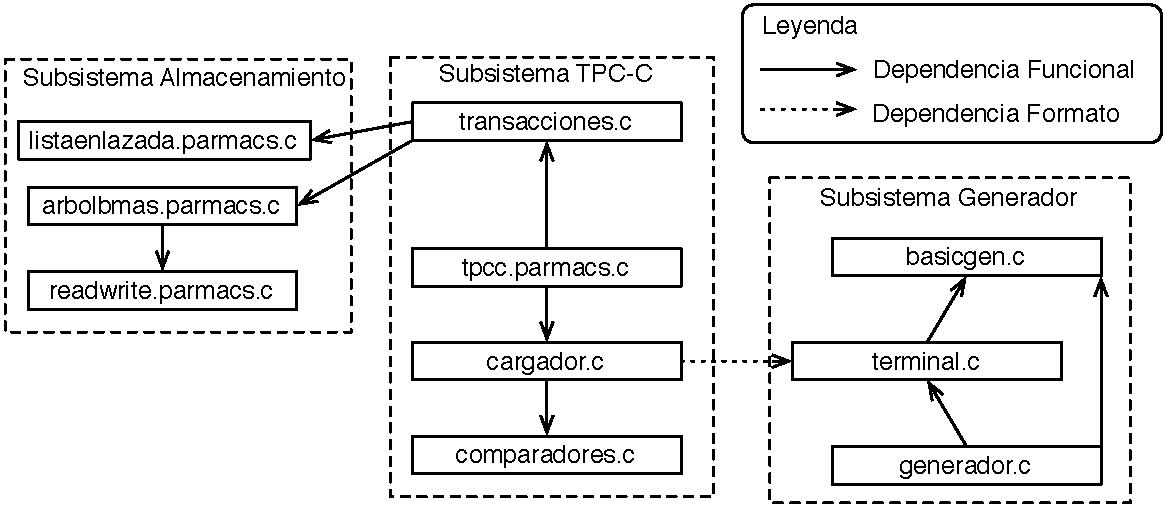
\includegraphics[width=\linewidth]{cap4/diagrama-dependencias.pdf}
\end{center}
\caption{Diagrama de dependencias entre m�dulos.}
\label{fig:diagrama-dependencias}
\end{figure}

\begin{itemize}
\item \textbf{Subsistema de almacenamiento}: que incluye los componentes
	\begin{itemize}
	\item Componente: \textit{�rbol B+}.
		\begin{itemize}
		\item Interfaz: \texttt{arbolbmas.h}
		\item Implementaci�n: \texttt{arbolbmas.parmacs.c
		readwrite.parmacs.c}
		\item Otras cabeceras: \texttt{arbolbmas-priv.h
		readwrite.parmacs.h}
		\end{itemize}
	\item Componente: \textit{Lista enlazada}
		\begin{itemize}
		\item Interfaz: \texttt{listaenlazada.parmacs.h}
		\item Implementaci�n: \texttt{listaenlazada.parmacs.c}
		\end{itemize}
	\end{itemize}
\item \textbf{Subsistema TPC-C}
	\begin{itemize}
	\item Componente \textit{Administrador}
		\begin{itemize}
		\item Implementaci�n: \texttt{tpcc.parmacs.c cargador.c comparadores.c}
		\item Otras cabeceras: \texttt{registros.h cargador.h}
		\end{itemize}
	\item Componente \textit{Servidor}
		\begin{itemize}
		\item Interfaz {transacciones.h}
		\item Implementaci�n {transacciones.c tpcc.parmacs.c}
		\end{itemize}
	\end{itemize}
\item \textbf{Subsistema Generador} s�lo con un componente: \textit{Generador}
	\begin{itemize}
	\item Interfaz: \texttt{terminal.h}
	\item Implementaci�n: \texttt{generador.c terminal.c basicgen.c}
	\end{itemize}
\end{itemize}

Las dependencias entre los diferentes m�dulos en los que est� dividio el c�digo
fuente asi como el subsistema al que pertenecen, se pueden observar en la figura
\ref{fig:diagrama-dependencias}.



\section{Subsistema de almacenamiento}
\subsection{Fundamentos de listas enlazadas}
Una lista enlazada es una colecci�n de elementos o nodos, en donde cada nodo
contiene unos datos y un enlace al nodo siguiente. La lista enlazada es una de
las estructuras din�micas m�s simples que implementa de manera vers�til una
lista din�mica de elementos donde continuamente se a�aden o se borran elementos.

Un nodo de la lista enlazada se define en la figura \ref{fig:nodolista}
\begin{figure}[htb]
\begin{center}
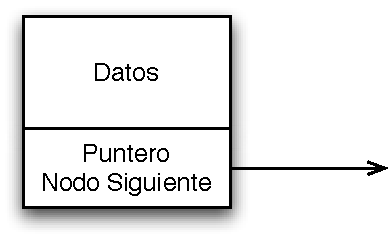
\includegraphics[width=3cm]{cap4/nodo-le.pdf}
\end{center}
\caption{Nodo de una lista enlazada}
\label{fig:nodolista}
\end{figure}

De tal manera que cuando se enlazan varios nodos obtenemos la estructura de la
figura \ref{fig:listaenlazada}

\begin{figure}[htb]
\begin{center}
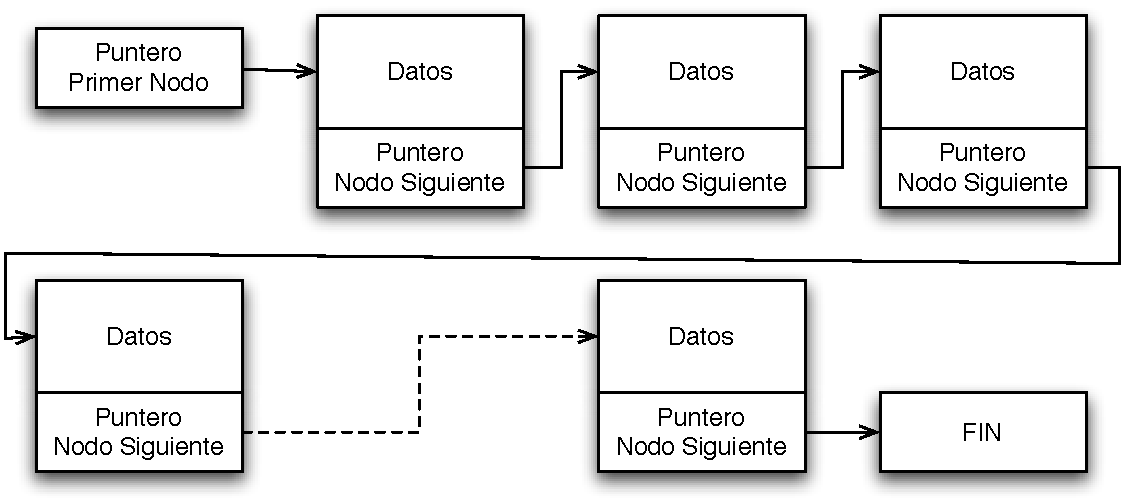
\includegraphics[width=\textwidth]{cap4/listaenlazada.pdf}
\end{center}
\caption{Estructura de lista enlazada}
\label{fig:listaenlazada}
\end{figure}

Dicha estructura no tiene porqu� estar ordenada, aunque a veces encontraremos
modificaciones como: que los datos tengan un orden en la lista, o exista un
puntero al �ltimo nodo de la lista
\subsubsection{Operaci�n de b�squeda}
La operaci�n de b�squeda en las listas enlazadas es una de las m�s costosas,
debido a que la b�squeda es secuencial y de orden n, es decir, hay que recorrer
todos los nodos para encontrar el que buscamos; en el peor de los casos, est�
ordenada o no, tengamos acceso desde el final o no, si buscamos un dato que no
se encuentra en la lista acabaremos recorriendo todos los nodos.

El procedimiento es el siguiente:
\begin{enumerate}
\item Colocarse en el primer nodo de la lista.
\item Comprobar si los datos son los que buscamos.
\item Si lo son, hemos terminado.
\item Si no lo son, colocarse en el siguiente nodo; si el nodo no es final
volver al segundo punto.
\item Si el nodo siguiente es el final, hemos terminado de manera no
satisfactoria.
\end{enumerate}

\subsubsection{Operaci�n de Inserci�n}
Una de las ventajas de las listas enlazadas es que no hace falta desplazar los
elementos cuando se insertan (ni cuando se borran). Para insertar un nuevo valor
en la lista enlazada existen dos maneras: al principio de la lista, tras alg�n
valor de la lista (lista ordenada).

Inserci�n al principio de la lista:
\begin{enumerate}
\item Obtener un nuevo nodo y almacenar el valor en la parte datos de dicho
nodo.
\item En este nuevo nodos, en la parte del puntero al nodo siguiente, almacenar
el valor de la variable \textit{puntero al primer nodo}.
\item Actualizar la variable \textit{puntero al primer nodo} con la direcci�n
del nuevo nodo creado.
\end{enumerate}

Inserci�n tras un valor de la lista:
\begin{enumerate}
\item Obtener un nuevo nodo y almacenar el valor en la parte datos de dicho 
nodo.
\item Buscar entre que dos nodos insertar, dichos nodos los llamaremos, anterior
y siguiente.
\item Del nodo anterior, actualizar el valor de su puntero al nodo siguiente a
la direcci�n del nuevo nodo.
\item En el nuevo nodo, actualizar el valor de su puntero al nodo siguiente a la
direcci�n del nodo siguiente.
\item Si siguiente es el primer nodo, no hay anterior, y procederemos como
cuando insertamos al principio de la lista.
\item Si anterior es el �ltimo nodo, no existe siguiente, por lo que en el nuevo
nodo, su puntero al siguiente nodo apuntar� a FIN.
\end{enumerate}

\subsubsection{Operaci�n de borrado}
En este caso tambi�n tenemos que considerar dos alternativas: borrar el primero,
o borrar un nodo intermedio.

Borrar el primer nodo:
\begin{enumerate}
\item Hacer que la variable \textit{puntero al primer nodo} apunte al nodo
siguiente del nodo apuntado originalmente.
\item Destruir el nodo desenlazado.
\end{enumerate}

Borrar un nodo intermedio:
\begin{enumerate}
\item Encontrar el nodo a borrar, en dicha b�squeda habr� dos nodos: el anterior
al nodo que queremos borrar, y el siguiente al nodo que queremos borrar.
\item Actualizar el puntero al nodo siguiente del nodo anterior al que queremos
borrar, y ponerle el valor de la direcci�n del nodo siguiente al que queremos
borrar.
\item Destruir el nodo desenlazado.
\item Si el nodo que queremos borrar es el primero, actuaremos como en el caso
de borrar el primer nodo.
\item Si el nodo que queremos borrar es el �ltimo, haremos que en el nodo
anterior al que queremos borrar, su puntero al nodo siguiente, apunte a FIN.
\end{enumerate}

\subsection{Sincronizaci�n de la lista enlazada}
Cuando se habla de sincronizar se habla de que varios procesos o hilos de
ejecuci�n puedan interactuar a la vez y sin interferencias con la misma
estructura de datos. El hecho de no controlar que muchos procesos accedan a la
estructura, no ocasionar�a problemas si todos leen la estructura, pero en el
momento que uno o m�s procesos intenten modificarla, pueden existir problemas.

Por ejemplo, si dos procesos A y B, quieren a�adir al final un nodo a trav�s de un
puntero de final de cola puede ocurrir que desaparezca uno de los nodos
insertados.

\begin{table}
\begin{tabularx}{\linewidth}{|X|X|}
\hline
\textbf{Proceso A} & \textbf{Proceso B} \\
\hline
Obtiene el valor del puntero al �ltimo nodo & \\
&Obtiene el valor del puntero al �ltimo nodo \\
Accede al �ltimo nodo y actualiza su siguiente nodo al nuevo nodo de A & \\
&Accede al �ltimo nodo y actualiza su siguiente nodo al nuevo nodo de B\\
&Actualiza el puntero al �ltimo nodo con el nuevo nodo de B \\
Actualiza el puntero al �ltimo nodo con el nuevo nodo de A & \\
\hline
\end{tabularx}
\caption{Ejemplo de c�mo corromper una lista enlazada con dos procesos}
\label{tab:le-corrupta}
\end{table}

Como se puede observar en el cuadro \ref{tab:le-corrupta}, nuestra estructura de
datos ha acabado corrupta ya que, el pen�ltimo nodo apunta al nodo a�adido por
B, pero el puntero del �ltimo nodo apunta al nodo a�adido por A; esto hace que
la estructura quede inservible, y si se ejecutan m�s operaciones sobre la misma
el resultado puede ser inesperado y no el deseado.

\subsubsection{Modelo de sincronizaci�n}
En el benchmark TPC-C la �nica tabla que utiliza la lista enlazada es la de
\textit{hist�rico}, y no hace m�s que a�adir nodos al final a trav�s de un
puntero que apunta al �ltimo nodo. Para evitar problemas como los anteriores se
ha puesto un cerrojo a las operaciones sobre la lista de tal manera que: no
puede ejecutarse ninguna operaci�n sobre la lista si una anterior no ha
terminado. Al c�digo que se ejecuta entre que se adquiere y se libera un bloqueo
de este tipo se le llama \textit{secci�n cr�tica}

En este caso el ejemplo anterior quedar�a como se puede observar en el cuadro \ref{tab:le-correcta}.
\begin{table}
\begin{tabularx}{\linewidth}{|X|X|}
\hline
\textbf{Proceso A} & \textbf{Proceso B} \\
\hline
Obtiene el cerrojo de la lista enlazada & \\
Obtiene el valor del puntero al �ltimo nodo & \\
&Intenta obtener el cerrojo de la lista enlazada, pero como ya est�
asignado se queda a la espera. \\
Accede al �ltimo nodo y actualiza su siguiente nodo al nuevo nodo de A & \\
Actualiza el puntero al �ltimo nodo con el nuevo nodo de A & \\
Libera el cerrojo & \\
&Despierta del bloqueo ya que A lo ha liberado, y obtiene el cerrojo \\
&Accede al �ltimo nodo y actualiza su siguiente nodo al nuevo nodo de B\\
&Actualiza el puntero al �ltimo nodo con el nuevo nodo de B \\
&Libera el cerrojo \\
\hline
\end{tabularx}
\caption{Ejemplo de inserci�n ordenada con dos procesos}
\label{tab:le-correcta}
\end{table}

Como se puede ver, ahora B accede al puntero del �ltimo nodo real, y lo que se
ha conseguido con este cerrojo es secuenciar las operaciones sobre la lista
enlazada.

\subsection{Implementaci�n de la lista enlazada}
Esta lista enlazada implementa inserci�n por el final y borrado por el
principio, aunque en el benchmark TPC-c no se usa el borrado por el principio.
Tambi�n incluye registros gen�ricos de tama�o N, que se explicar�n m�s adelante.

\subsubsection{Estructuras y tipos de datos}
Las estructuras y tipos de datos utilizadas, est�n declaradas en 
\textit{listaenlazada.parmacs.h}.
\paragraph{$\triangleright$ struct struct\_LENodo}
Estructura para manejar los enlaces al nodo siguiente. Esto es lo que se a�adir�
a los registros gen�ricos que se quieran insertar en la lista. Contenido:
\begin{itemize}
\item \texttt{struct struct\_LENodo *siguiente;} Puntero al siguiente elemento
de la lista. Con valor NULL cuando no hay m�s nodos en la lista.
\end{itemize}

\paragraph{$\triangleright$ struct struct\_ListaEnlazada}
Almacena la informaci�n necesaria para manejar la lista. Contenido:
\begin{itemize}
\item \texttt{struct struct\_LENodo *principio;} Puntero al primer nodo de la
lista, o NULL cuando est� vac�a.
\item \texttt{struct struct\_LENodo *fin;} Puntero al �ltimo nodo de la lista, o
NULL cuando est� vac�a.
\item \texttt{int regsize;} Tama�o del registro gen�rico usado
\item \texttt{LOCKDEC(bloqueo);} Cerrojo de la lista.
\end{itemize}

\paragraph{$\triangleright$ LENodo}
Se define el tipo de dato LENodo de la siguiente manera:\\
\texttt{typedef struct struct\_LENodo LENodo;}
\paragraph{$\triangleright$ ListaEnlazada}
Se define el tipo de dato ListaEnlazada de la siguiente manera:\\
\texttt{typedef struct struct\_ListaEnlazada ListaEnlazada;}


\subsubsection{Interfaz de uso}
Para utilizar la implementaci�n de la lista enlazada, se han dispuesto las
siguientes funciones declaradas en \texttt{listaenlazada.parmacs.h}.
\paragraph{$\triangleright$ le\_nueva}
\begin{itemize}
\item Declaraci�n: \texttt{ListaEnlazada *le\_nueva(int regsize)}
\item Descripci�n: Inicializa un identificador de lista enlazada. 
	\begin{itemize} 
	\item Se inicializan los punteros a null
	\item Se almacena el tama�o del registro.
	\item Se inicializa el cerrojo.
	\end{itemize}
\item Par�metros:
	\begin{itemize}
	\item \texttt{int regsize} (entrada): Tama�o del registro de datos
	gen�rico con el que trabajar.
	\end{itemize}
\item Devuelve: un puntero a la estructura de lista enlazada, que estar� 
inicializada como vac�a.
\end{itemize}

\paragraph{$\triangleright$ le\_insertar\_final}
\begin{itemize}
\item Declaraci�n: \texttt{void le\_insertar\_final(ListaEnlazada *lista,void
*registro)}
\item Descripci�n: (funci�n sincronizada) Inserta al final de la lista.
	\begin{itemize}
	\item Reserva memoria para el registro y la estructura de nodo.
    	\item Actualiza los punteros para colocar el nodo.
    	\item Copia los datos del nodo.
	\end{itemize}
\item Par�metros:
        \begin{itemize}
        \item \texttt{ListaEnlazada *lista} (entrada): Lista enlazada sobre la
	que operar.
        \item \texttt{void *registro} (entrada): Puntero al registro que
	insertar en la lista.
        \end{itemize}
\end{itemize}

\paragraph{$\triangleright$ le\_borrar\_primero}
\begin{itemize}
\item Declaraci�n: \texttt{int le\_borrar\_primero(ListaEnlazada *lista, void
*registro)}
\item Descripci�n: (funci�n sincronizada) Borra el primer elemento de la lista y lo devuelve.
	\begin{itemize}
    	\item Primero comprueba si la lista est� vac�a.
    	\item En caso de no estarlo, copia los datos al registro.
    	\item Y luego actualiza los punteros internos.
	\end{itemize}
\item Par�metros:
        \begin{itemize}
        \item \texttt{ListaEnlazada *lista} (entrada): Lista enlazada sobre la
	que operar.
        \item \texttt{void *registro} (salida): Lugar donde depositar el
	registro borrado.
        \end{itemize}
\item Devuelve: Un entero indicando el resultado de la operaci�n.
	\begin{itemize}
	\item \texttt{OP\_OK} Operaci�n Correcta.
	\item \texttt{OP\_NODATA} Sin datos debido a que la lista estaba vac�a.
	\end{itemize}
\end{itemize}

\paragraph{$\triangleright$ le\_destruir}
\begin{itemize}
\item Declaraci�n: \texttt{void le\_destruir(ListaEnlazada *lista)}
\item Descripci�n: Va borrando todos los nodos uno a uno.
\item Par�metros:
        \begin{itemize}
        \item \texttt{ListaEnlazada *lista} (entrada): Lista enlazada sobre la
	que operar.
        \end{itemize}
\end{itemize}

\subsubsection{Peculiaridades}
La primera peculiaridad en esta lista y que se aplicar� tambi�n en el �rbol B+,
es que se habla de \textit{registros gen�ricos}. Un registro gen�rico es aquel
que puede albergar cualquier tipo de dato, por tanto la lista no tiene en cuenta
el contenido de los datos para su funcionamiento interno.

Si bien se ha definido como un nodo de la lista la estructura struct\_LENodo,
que s�lo tiene un puntero al nodo siguiente. A la hora de reservar memoria se
reserva espacio para
\begin{itemize}
\item El puntero al nodo siguiente (lo que es la estructura LENodo).
\item Los datos (el tama�o est� indicado por regsize).
\end{itemize}

Por lo que tendremos una asignaci�n como la siguiente (extra�da de la funci�n
le\_insertar\_final):
\texttt{newrecord=G\_MALLOC(lista->regsize+sizeof(LENodo));}

A la hora de obtener los datos de un registro cualquiera, no tenemos m�s que,
dado el puntero del registro, desplazarnos el tama�o del puntero y leer a partir
de ah�: \texttt{memcpy(registro,tmp+1,lista->regsize);}

El segundo punto interesante, y que tambi�n se aplicar� en el �rbol B+, es que a
la hora de a�adir datos, aunque se le pase una zona de memoria con los datos, la
lista enlazada reserva una zona de memoria compartida para guardar ese dato, con
lo que queda accesible por los dem�s procesos.

\subsection{Fundamentos de �rboles B+}
Ya se ha hablado (pag. \pageref{sec:arbolbmasbasico}) sobre la estructura de un
�rbol B+; si decimos que un �rbol B+ es de orden $p$ decimos que:
\begin{itemize}
\item Si el nodo es interno tiene $p-1$ claves y $p$ enlaces.
\item Si el nodo es hoja, tiene $p-1$ claves y enlaces.
\end{itemize}

Los nodos de un �rbol B+ siguen la estructura de la figura \ref{fig:abm-nodos}
\begin{figure}[htb]
\begin{center}
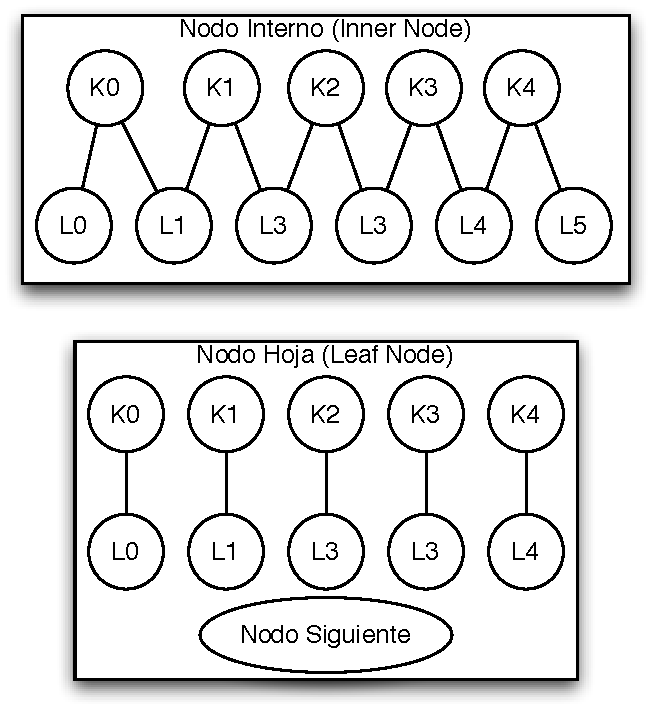
\includegraphics[width=8cm]{cap4/abm-nodos.pdf}
\end{center}
\caption{Nodos de un �rbol B+}
\label{fig:abm-nodos}
\end{figure}

La estructura que sirva para manejar un �rbol B+ al menos tendr� un puntero al
nodo ra�z, y un puntero al primer nodo hoja, ya que los nodos hoja est�n unidos
formando una lista enlazada, que es de gran utilizad cuando se realizan
b�squedas no indexadas.

Aunque se han estudiado muchas mejoras \cite{672375}, \cite{vilho04}, sobre todo
en lo referente a la relaci�n: eficiencia de cach� respecto al acceso a los
nodos, en este an�lisis y en esta implementaci�n s�lo se utilizan los fundamentos
b�sicos de arboles B+.

\subsubsection{B�squeda indexada}
La b�squeda a trav�s de un campo clave es el punto fuerte de los arboles B+,
entre millones de entradas se puede acceder a aquella que andamos buscando en
cuesti�n de mil�simas de segundo. Para entender las razones de esta afirmaci�n,
se va explicar un ejemplo.

Supongamos que tenemos un �rbol B+ de orden 51, es decir, aquel �rbol cuyos
nodos internos tienen 51 enlaces y 50 claves, y cuyos nodos hoja tienen 50
enlaces y 50 claves. Llamaremos altura del �rbol, a los nodos que hay que
recorrer desde el ra�z, hasta llegar a un nodo hoja, ambos inclusive. La
cantidad de datos que podemos almacenar es la siguiente:
\begin{itemize}
\item Altura 1: 50 registros. S�lo existe un nodo, el ra�z que es a su vez nodo
hoja.
\item Altura 2: $51*50=2.550$ registros. Del nodo ra�z parten 51 enlaces a nodos
hoja que a su vez pueden almacenar 50 registros.
\item Altura 3: $51*51*50=130.050$ registros. Del nodo ra�z parten 51 enlaces a nodos
internos, que tienen 51 enlaces a nodos hoja; estos �ltimos albergan 50 enlaces
a registros.
\item Altura 4: $51*51*51*50=6.632.550$ registros. Ya tenemos varios millones de
registros con solo 4 alturas.  
\end{itemize}

Nos quedaremos con el �rbol B+ de orden 51 y de 4 alturas, se supone que est�
totalmente lleno y que por lo tanto podremos acceder a los m�s de 6 millones de
registros. La operaci�n de b�squeda a partir de una clave $K$ es la siguiente:

\begin{enumerate}
\item Se accede al nodo ra�z y se marca como nodo actual.
\item Dado que las claves del nodo actual est�n ordenadas, se busca la clave $K$
entre todas las claves del nodo actual mediante una \textit{b�squeda binaria}, 
si no se encuentra, se dice la posici�n
aproximada, es decir, entre que dos claves se encuentra.
\item Entre la clave $K_{i-1}$ y la clave $K_i$ se encuentra el enlace $L_i$
que nos lleva al nodo cuyas claves son: mayores que $K_{i-1}$ y menores o
iguales que $K_i$. (fig. \ref{fig:abm-busqueda1})
\begin{figure}[htb]
\begin{center}
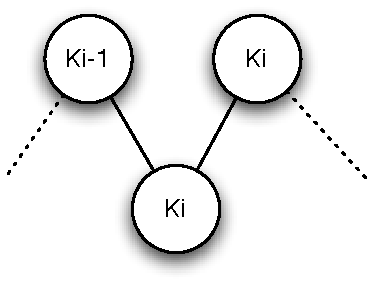
\includegraphics[width=3cm]{cap4/abm-busqueda1.pdf}
\end{center}
\caption{Estructura de un nodo interno}
\label{fig:abm-busqueda1}
\end{figure}
\item La posici�n aproximada es aquella $i$ tal que: $K_{i-1} < K \leq K_i$.
\item Accedemos al nodo apuntado por la posici�n $i$ ($L_i$), y lo llamamos nodo
actual.
\item Si el nodo es hoja, repetimos desde el punto dos y accederemos al dato.
\item Si el nodo es interno, volvemos al punto 2.
\end{enumerate}

Para recorrer los 4 niveles del nodo se han hecho 4 b�squedas binarias entre 50
elementos, que obviamente son mucho menos costosas que una b�squeda binaria entre
6 millones de elementos. De ah� que acceder a un registro entre varios millones
s�lo conlleve unos pocos milisegundos.

\subsubsection{B�squeda no indexada}
Este es el punto d�bil de los �rboles B+, si no se posee un campo clave por el
cual buscar un nodo en el �rbol, hay que recorrer todos los nodos. Aun as�, el
�rbol B+ presenta cierta facilidad para realizar esa tarea; debido a que todos
sus nodos hoja est�n enlazados entre si, y solo los nodos hoja contienen enlaces
a los datos, obtenemos una \textit{lista simplemente enlazada} con los nodos
hoja, que podremos recorrer para encontrar el dato buscado.

Utilizando el ejemplo anterior de un �rbol B+ de orden 51 con 4 niveles, y
suponiendo el peor caso, y es que el nodo buscado est� al final de la lista
enlazada. Dado que no se est� buscando por clave y por lo tanto no se puede utilizar la b�squeda
binaria en cada nodo, se tendr�an que realizar m�s de 6 millones de
comparaciones antes de llegar al nodo final.

El algoritmo de b�squeda ser�a el siguiente:
\begin{enumerate}
\item Se accede al primer nodo hoja y se le nombra: nodo actual.
\item Se busca uno a uno entre los registros apuntados por el nodo actual el
dato que buscamos.
\item Si se encuentra, se finaliza la b�squeda.
\item Si no se encuentra, se utiliza el puntero al nodo siguiente, y hacemos del
nodo siguiente el nodo actual; por �ltimo volvemos al punto 2.
\end{enumerate}

\subsubsection{Inserci�n}
La inserci�n de un registro extra en un �rbol B+ puede ser tan costosa como
muy simple; no es que sea una de las operaciones m�s peligrosas a la hora de
manejar esta estructura pero sin conviene hacerse met�dicamente para evitar
errores.

Toda inserci�n en un �rbol B+ comienza con una b�squeda del nodo hoja donde
debiera encontrarse la clave del registro que queremos insertar. Si localizado
el nodo hoja, este tiene espacio suficiente para albergar el nuevo registro, el
algoritmo es el siguiente.
\begin{enumerate}
\item Lo primero es realizar una b�squeda binaria para conocer en que posici�n
debiera insertarse el registro actual. Utilizando la funci�n de b�squeda binaria
aproximada que se utiliz� en la b�squeda indexada, obtenemos dicha posici�n.
\item Si el nodo admite claves duplicadas y la clave existe, continuamos
normalmente; pero si no las admite y la clave existe, se anula la inserci�n.
\item Si la posici�n de inserci�n es $i$ en el nodo hoja, desplazamos todos los
pares de: $(K_j,Lregistro_j)$ una posici�n a la derecha desde
$j=ocupados$ (que simboliza la cantidad actual de enlaces ocupados en el nodo)
hasta $j=i$, lo hacemos al rev�s (de derecha a izquierda) para que la operaci�n $K_{j+1}=K_j,
Lregistro_{j+1}=Lregistro_j$ no sobreescriba datos existentes.
\item Por �ltimo, insertamos nuestro nuevo registro copiando la clave en $K_i$ y
actualizando el puntero al registro $Lregistro_i=NuevoRegistro$.
\end{enumerate}

Es una operaci�n m�s complicada cuando el nodo hoja est� lleno, en ese caso hay
que dividir el nodo hoja, para obtener dos nodos hoja llenos hasta la mitad, y
as� poder insertar en uno de los dos nuevos nodos creados. La divisi�n de un
nodo hoja se realiza de esta manera:
\begin{enumerate}
\item Dado un nodo hoja lleno, se busca \textit{la mitad} de dicho nodo.
\item La mitad de dicho nodo se indica como $i$. Se crea un nuevo nodo vac�o.
\item Se mueven los datos: de $i$ hasta el final del nodo al nuevo nodo creado.
Tenemos dos nodos: \textit{izquierdo} (de $0$ a $i-1$) y \textit{derecho} (de
$i$ hasta el final).
\item Al tener un nuevo nodo hoja, hace falta enlazarlo con el nodo anterior,
que es un nodo interno. Recordemos que los nodos internos tienen claves para
indicar que camino tomar, as� que al a�adir un nuevo enlace en el nodo superior,
necesitaremos una nueva clave para guiar las b�squedas.
\item Dada una clave $K_j$ todos aquellos valores menores o iguales se
encuentran en el enlace $L_j$ y los mayores en el enlace $L_{j+1}$
\item Utilizamos la �ltima clave del nodo izquierdo como clave de uni�n.
\end{enumerate}

Se ha dejado el algoritmo a la mitad para resumir los pasos hechos hasta el
momento: cuando un nodo hoja esta lleno, se divide por la mitad en dos nodos:
izquierdo y derecho, siendo la ultima clave del izquierdo la clave de uni�n.
Ahora hay que introducir dicha clave en el nodo superior, que es un nodo
interno.

\begin{enumerate}
\item Nos posicionamos en el nodo interno superior al nodo hoja, y buscamos la
posici�n $i$ por la que se accede al nodo hoja.
\item Como hemos dividido anteriormente, desde esa posici�n $i$ s�lo se accede a
la mitad de los valores por lo que, idealmente, debi�ramos colocar la clave de
uni�n como $K_i$ ya que en el nodo izquierdo est�n los valores menores o iguales
que $K_i$.
\item Para poder realizar esto movemos todas las claves desde $K_ultima$ a $K_i$
un lugar a la derecha: $K_{j+1}=K_j$.
\item Realizamos lo mismo con los enlaces pero desde $L_ultimo$ a $L_{i+1}$.
\item Al realizar este desplazamiento de enlaces dejamos un hueco para insertar
un enlace al nodo derecho (fig. \ref{fig:abm-insertar1}).
\begin{figure}[htb]
\begin{center}
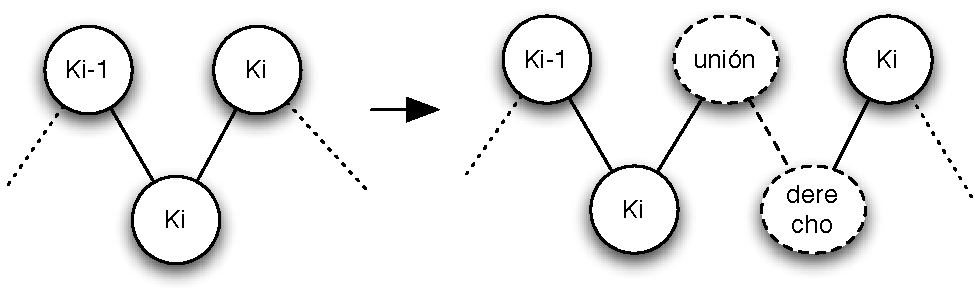
\includegraphics[width=\linewidth]{cap4/abm-insertar1.pdf}
\end{center}
\caption{Inserci�n de una clave de uni�n en un nodo interno}
\label{fig:abm-insertar1}
\end{figure}
\end{enumerate}

Una vez hecho esto, no hab�amos insertado aun el registro en el nodo hoja, y al
dividir el nodo hoja, s�lo nos queda seleccionar si va en el izquierdo o en el
derecho y realizar una inserci�n normal en el nodo hoja adecuado. No olvidar
completar la lista enlazada, el nodo izquierdo apunta al nuevo nodo derecho, y
el nuevo nodo derecho apunta donde antes apuntaba el viejo nodo izquierdo, es
decir, una inserci�n entre medias de una lista simplemente enlazada.

Por �ltimo puede ocurrir un problema, y es que al ir a insertar en el nodo
interno superior, este est� lleno. La t�cnica a aplicar es la misma: dividir el
nodo interno, obtener una clave de uni�n e insertar la clave de uni�n en el nodo
interno superior; pero hay que tener cuidado con ciertos detalles.
\begin{enumerate}
\item Los nodos internos tienen distinto n�mero de claves que de enlaces, y su
disposici�n es como la de \textit{varios tri�ngulos juntos}, siendo el v�rtice
superior la clave y los dos inferiores los enlaces. A la hora de dividir un nodo
interno por la mitad, el tri�ngulo se dividir� en dos, y la clave del v�rtice
superior desaparecer� del nodo y pasar� a ser la clave de uni�n.
\item Si dividimos el nodo ra�z, hay que insertar un nodo interno nuevo y con
s�lo dos enlaces y una clave: la clave de uni�n, y los enlaces a las dos partes
del nodo dividido.
\end{enumerate}

Para la tarea de inserci�n, muchas veces es �til tener punteros de navegaci�n en
los nodos: nodo anterior, nodo siguiente, etc. Estos punteros pueden estar en el
propio nodo, o los podemos ir almacenando seg�n vamos descendiendo en el �rbol. 

\subsubsection{Borrado}
Al igual que con la inserci�n el borrado es una operaci�n que puede ser sencilla
simplemente borrando una entrada en un nodo hoja; o bastante compleja,
necesitando borrar varias entradas en varios nodos internos. Se va a explicar
igual que se indic� la inserci�n, comenzando por un borrado simple en un nodo
hoja; el algoritmo es el siguiente:

\begin{enumerate}
\item Dada una clave $K$, buscar el nodo hoja que debiera contener la clave $K$.
\item Si no se encuentra, hemos terminado.
\item Si la encontramos, estar� en la posici�n $i$ del nodo hoja.
\item Desplazar los pares de clave y enlace $(K_j,L_j)$ desde $i+1$ hasta
$ultimo$, una unidad a la izquierda: $K_j=K_{j+1}$
\item Liberar la memoria del registro asociado a la vieja clave $K_i$.
\end{enumerate}

En este momento puede ocurrir que el nodo rebase el l�mite de tama�o m�nimo. Si
bien se hab�a dicho que un nodo como m�nimo puede tener $(maximo/2)$ claves; es
muy normal experimentar con dicho l�mite para optimizar el funcionamiento del
�rbol en un entorno concreto.

Se supondr� que el nodo ha rebasado su l�mite de tama�o m�nimo y hay que hacer
\textit{algo} para solucionarlo. Ese algo consiste en dos soluciones:
\begin{itemize}
\item \textit{Balancear}: Dados dos nodos, se balancea su contenido entre los
dos, terminando ambos nodos con el mismo n�mero de claves y enlaces ocupados.
\item \textit{Fusionar}: Dados dos nodos, se fusiona uno con otro,
desapareciendo el primero, y pasando su contenido a formar parte del segundo.
\end{itemize}

En este caso hay que tener \textit{anotados} los nodos izquierdo y derecho del
nodo hoja donde nos encontramos, as� como si el padre de dichos nodos es el
mismo que el del nodo actual. Hay que tener esto en cuenta ya que a la hora de
balancear dos nodos, o de fusionar dos nodos, s�lo se balancean o fusionan
aquellos nodos que tengan el mismo padre, para as� solo alterar un enlace y una
clave de dicho padre.

Las situaciones con las que nos podemos encontrar y la acci�n a tomar son las
indicadas en el cuadro \ref{tab:abm-borrar}.

\begin{table}
\begin{tabularx}{\linewidth}{|X|X|X|}
\hline
\bf Vecino izquierdo & \bf Vecino derecho& \bf Acci�n \\
\hline
\hline
No esta lleno    & No Hay	 & Fusi�n del actual con el izquierdo\\
\hline
Lleno            & No Hay        & Balancear el actual con el izquierdo\\
\hline
No Hay&	No esta lleno	&Fusi�n del actual con el derecho\\
\hline
No Hay& Lleno&	Balancear el actual con el izquierdo\\
\hline
Otro padre distinto al del nodo actual&	Mismo padre Y puede admitir&
Fusi�n del actual con el derecho\\
\hline
Otro padre distinto al del nodo actual&	Mismo padre Y esta lleno&
Balancear el actual con el derecho\\
\hline
Mismo padre Y puede admitir&Otro padre distinto al del nodo actual&
Fusi�n del actual con el izquierdo\\
\hline
Mismo padre Y esta lleno & Otro padre distinto al del nodo actual&
Balancear el actual con el izquierdo\\
\hline
Mismo padre Y puede admitir&Mismo padre Y puede admitir	&Fusi�n
del actual con el derecho (podr�a ser izquierdo tambi�n)\\
\hline
Mismo padre Y lleno	&Mismo padre Y puede admitir	&Balancear el
actual y el izquierdo\\
\hline
Mismo padre Y puede admitir&Mismo padre Y lleno	&Balancear el actual con el derecho\\
\hline
\end{tabularx}
\caption{Resumen de acciones de borrado}
\label{tab:abm-borrar}
\end{table}

El algoritmo de fusi�n es el siguiente:
\begin{enumerate}
\item Dados dos nodos izquierdo y derecho, se fusiona siempre hacia la
izquierda.
\item Se mueven todos los datos del nodo derecho al izquierdo.
\item Se elimina el nodo izquierdo.
\item Se anota que han ocurrido cambios para m�s tarde borrar el enlace del nodo
superior al nodo izquierdo que ya no existe.
\end{enumerate}

Y para el balanceo:
\begin{enumerate}
\item Dados dos nodos: izquierdo y derecho, se comprueba la ocupaci�n de cada
uno.
\item La suma de los dos tama�os entre 2 es el nuevo tama�o de ambos nodos.
\item La cantidad a desplazar es el tama�o del nodo m�s grande menos el tama�o
nuevo.
\item Si el izquierdo es m�s grande que el derecho, se mueven nodos y enlaces de
izquierda a derecha.
\item Si el derecho es m�s grande, se mueven nodos y enlaces del nodo derecho al
izquierdo.
\end{enumerate}

El algoritmo de borrado completo es el siguiente:
\begin{enumerate}
\item Continuando con el caso anterior se ha buscado y borrado un elemento de un nodo hoja.
\item Despu�s de borrar hay \textit{pocos} elementos.
\item Se selecciona una acci�n del cuadro \ref{tab:abm-borrar}
\item Si la acci�n ha sido balancear, se termina.
\item Si la acci�n ha sido fusionar, hay un nodo menos y hay que quitar un
enlace del nodo superior.
\item Volver a aplicar el algoritmo de borrado completo en el nodo superior.
\end{enumerate}

Se puede observar que este algoritmo es recursivo a la hora de descender, ya que
se anotan: nodos izquierdos y derechos as� como sus padres. Y luego se retrocede
ese camino recursivo borrando entradas de los nodos si han sucedido fusiones de
nodos, ya que en este caso hay que eliminar un enlace.

La fusi�n se produce siempre hacia la izquierda, lo que garantiza que el �rbol
siempre estar� equilibrado: se ir�n borrando nodos hoja a la vez que se ajusta
el contenido de los nodos superiores; pero esto hace tambi�n dif�cil que el
�rbol reduzca su nivel. Por ejemplo, en el �rbol de orden 51 con 4 niveles,
hace falta dejar al nodo ra�z con s�lo un enlace para que desaparezca (y as�
eliminar un nivel), esto supone eliminar $50*51*51*50=6.502.500$ registros, para que
el �rbol tenga ahora $51*51*50=130.050$ registros.

\subsection{Sincronizaci�n del �rbol B+}
Dado que los �rboles B+ se utilizan en sistemas de bases de datos como �ndices,
se han analizado diferentes formas \cite{rao00making} de mejorar la
sincronizaci�n y por lo tanto el bloqueo de accesos, a las estructuras de un
�rbol B+. El problema del acceso concurrente por parte de varios procesos o hilos
de ejecuci�n a la estructura del �rbol, ya no es dos simples enlaces que pueden
corromperse, sino millones de enlaces donde el hecho de que uno no indique el
nodo correcto puede suponer perder la mitad de la informaci�n almacenada.

\subsubsection{Primera aproximaci�n}
Una aproximaci�n a las t�cnicas de bloqueo pasa por analizar que operaciones
deseamos bloquear. En un principio y pensando que un proceso pueda estar leyendo
el �rea que otro proceso est� alterando, la primera soluci�n que se sugiere es:
\textit{poner un cerrojo por �rbol}, de tal manera que las operaciones se
realizan de manera secuencial y no ocurre una siguiente antes de que termine la
anterior.

Esta soluci�n evita todos los problemas pero es muy poco eficiente, debido a
que:
\begin{itemize}
\item Es muy habitual que varios procesos lean a la vez el �rbol. Esto no supone
en la realidad ning�n problema pero con esta aproximaci�n no es posible, por lo
que cada lector tiene que esperar a que el anterior termine.
\item Se tiene como ejemplo el �rbol anterior de orden 51 y 4 niveles, tenemos
m�s de 6 millones de registros. Si adem�s se tienen 16 procesos accediendo al �rbol
simult�neamente, con 6 millones de registros, la probabilidad de que de un nodo
hoja se borre a la vez que se lea es muy baja. Suponiendo que no hay que tocar
el �rbol nada m�s que para borrar la entrada de un nodo hoja sin fusionar o
balancear:
	\begin{itemize}
	\item Si bloqueamos el �rbol entero para una operaci�n de lectura,
	podr�amos estar realizando la operaci�n de borrado sin problemas.
	\item Si bloqueamos el �rbol entero para escritura y sabemos que no
	vamos a tener que fusionar ni balancear, podr�amos estar haciendo muchas
	otras lecturas que no hacemos.
	\end{itemize}
\item Esto �ltimo se aplica tambi�n a las inserciones si no hay que dividir el
nodo donde insertamos.
\end{itemize}

Analizando estos casos, se puede ver un problema bien conocido: existe una
estructura de datos en memoria com�n a varios procesos, unos procesos quieren
leer y otros escribir. Es el problema de los \textit{lectores escritores}

\subsubsection{Lectores Escritores}
La idea b�sica del problema de los lectores escritores es la siguiente:
bas�ndose en una estructura com�n:
\begin{itemize}
\item Varios procesos quieren leer y varios escribir.
\item Pueden existir varios lectores a la vez en esa estructura com�n.
\item S�lo puede existir un escritor operando en dicha estructura. Aunque muchos
lectores y escritores pueden estar esperando para realizar la operaci�n, s�lo un
escritor puede operar en el arbol, y cuando dicho escritor trabaja, ning�n otro
lector puede operar.
\end{itemize}

Soluciones se pueden encontrar en los libros de sistemas operativos
\cite{tanem98}, \cite{stal02}. Muchas de estas soluciones est�n
\textit{desequilibradas}, es decir, dan preferencia a los lectores o a los
escritores. La preferencia se asigna de tal manera que si hay preferencia a los
escritores, cuando llega un escritor, se salta la cola de espera de los lectores
y es el siguiente que entra a operar; o al rev�s, la preferencia de los
lectores, indica que un lector cuando se pone a la espera para operar en el
�rbol siempre se salta la cola de los escritores.

Esto puede provocar \textit{inanici�n}: que un escritor no llegue a escribir
nunca o que un lector no llegue a leer nunca, debido a que aunque est�n en la
cola a la espera de operar, siempre hay otra operaci�n que se salta dicha cola y
les mantiene indefinidamente a la espera.

Para evitar dicha inanici�n se ha utilizado un algoritmo lo m�s equilibrado
posible (cuadro \ref{tab:readwrite}). Se compone de:
\begin{itemize}
\item \textit{num\_lectores}: Una variable que controla el n�mero de lectores.
\item \textit{seccion\_critica}: Un cerrojo para acceder a dicha variable.
\item \textit{cola}: Un cerrojo que act�a como una cola donde se apuntan tanto lectores como
escritores.
\item Un cerrojo para los escritores.
\end{itemize}

\begin{table}
\begin{tabularx}{\linewidth}{|X|X|}
\hline
\multicolumn{1}{|c|}{\bf Lector} & \multicolumn{1}{c|}{\bf Escritor} \\
\hline
\hline
\tt LOCK(cola) & \tt LOCK(cola)\\
\tt LOCK(seccion\_critica) & \tt LOCK(bloqueo\_escritores)\\
\tt num\_lectores=num\_lectores+1 & \tt UNLOCK(cola)\\
\hhline{~-}
\tt if (num\_lectores == 1) & Realizar la escritura\\
\hhline{~-}
\tt \quad LOCK(bloqueo\_escritores)& \tt UNLOCK(bloqueo\_escritores)\\
\hhline{~-}
\tt UNLOCK(seccion\_critica) &\\
\tt UNLOCK(cola) & \\
\hhline{-}
Realizar la lectura correspondiente. & \\
\hhline{-}
\tt LOCK(seccion\_critica) & \\
\tt num\_lectores=num\_lectores-1 & \\
\tt if (num\_lectores == 0) & \\
\tt \quad UNLOCK(bloqueo\_escritores) & \\
\tt UNLOCK(seccion\_critica) & \\
\hline
\end{tabularx}
\caption{Algoritmo de lectores escritores equilibrados usando cerrojos}
\label{tab:readwrite}
\end{table}

La nomenclatura de las diferentes acciones de la soluci�n al problema lector
escritor son:
\begin{itemize}
\item \textit{Bloquear para leer}: ejecutar la primera parte del lector,
hasta justo antes de realizar la lectura correspondiente. Simboliza que se
quiere realizar una lectura.
\item \textit{Desbloquear lectura}: ejecutar la segunda parte del lector, justo
despu�s de la lectura correspondiente. Simboliza que la lectura ha finalizado.
\item \textit{Bloquear para escribir}: ejecutar la primera parte del escritor, hasta
justo antes de realizar la escritura correspondiente. Como antes, simboliza que
se quiere realizar una escritura.
\item \textit{Desbloquear escritura}: ejecutar la segunda parte del escritor (un
simple desbloqueo), justo despu�s de la escritura correspondiente. Simboliza que
la escritura ha finalizado.
\end{itemize}

Algunos casos con los que nos podemos encontrar son los siguientes, que adem�s
ayudar�n a entender el funcionamiento de esta soluci�n al problema lector
escritor.
\begin{itemize}
\item \textbf{S�lo lectores}: en este caso, como pueden existir m�ltiples
lectores accediendo de manera concurrente a los datos, cada lector aumenta en
uno la variable de n�mero de lectores; adem�s el primer lector impide a los
escritores entrar bloqueando el cerrojo de los escritores.
Al acabar su lectura decrementan en uno el contador de lectores y el �ltimo
lector que sale, abre el cerrojo de los escritores.
\item \textbf{Aparece un escritor}: 
\begin{enumerate}
\item En un momento dado, aparece un escritor,
junto con el resto de lectores se pone en la cola, pero mientras que los
lectores salen de la cola directamente, el escritor se queda bloqueado en su
cerrojo de escritores ya que, continuando con el punto anterior, hay muchos
lectores accediendo.
\item Como no ha desbloqueado el cerrojo de cola, en el preciso instante que se
queda bloqueado en su cerrojo de escritor, todas las nuevas peticiones, ya sean
de lectores o escritores se bloquean en el cerrojo de cola.
\item Con el tiempo, los lectores que hay dentro terminar�n su lectura, e ir�n
decrementando el contador.
\item Cuando el �ltimo lector salga, desbloquear� el cerrojo de los escritores,
y el lector liberar� la cola y realizar� su escritura. En este momento puede
intentar acceder un lector o un escritor.
\item Cuando el escritor termine, abrir� el cerrojo de escritura.
\end{enumerate}
\item \textbf{Justo despu�s del escritor, aparece un lector}
\begin{enumerate}
\item Cuando el escritor desbloquea la cola, entra un lector.
\item Ese lector es el primero, ya que recordemos que para que el escritor
entrase no tenia que haber ning�n lector.
\item El lector al ser el primero, intenta bloquear el cerrojo de escritores,
pero ya esta bloqueado dado que hay un lector dentro, y se queda a la espera.
\item Como se queda a la espera, el cerrojo de cola no se desbloquea y no pueden
entrar m�s operaciones.
\item Cuando el escritor termine abriendo dicho cerrojo de cola, el lector que
hab�a permanecido a la espera en dicho cerrojo se desbloquea dejando dicho
cerrojo bloqueado para nuevos escritores.
\end{enumerate}
\item \textbf{Justo despu�s del escritor, aparece otro escritor}
\begin{enumerate}
\item Ahora justo despu�s del escritor, en vez de un lector, aparece otro
escritor.
\item Pasa del cerrojo de la cola al cerrojo de escritores.
\item Como el cerrojo de escritores estaba bloqueado debido a que ya hay un
escritor dentro, se queda a la espera de que el escritor termine la operaci�n.
\item En dicha espera no libera el cerrojo de cola, por lo que las nuevas
operaciones se ponen a la espera en dicha cola.
\item Cuando el escritor inicial termina, desbloquea el cerrojo de escritores, y
el nuevo escritor comienza su operaci�n.
\item Si justo despu�s aparece un lector, es el caso anterior; y si aparece un
escritor, es este mismo caso.
\end{enumerate}
\end{itemize}

\subsubsection{Soluci�n aplicada al �rbol B+ implementado}
En el �rbol que se ha implementado se ha aplicado el problema de los lectores
escritores en 2 niveles:
\begin{itemize}
\item \textit{A nivel de �rbol}: se puede bloquear el �rbol para lectura o para
escritura.
\item \textit{A nivel de nodo hoja}: un nodo hoja se puede bloquear para lectura o para
escritura.
\end{itemize}

La idea de aplicar esta divisi�n en dos niveles es que muchas veces solamente se
necesita bloquear el nodo hoja para a�adir o borrar un dato, dejando el �rbol
intacto; por lo que no hay que bloquear el �rbol entero (millones de registros),
si solo necesitamos bloquear un nodo. Si a la hora de insertar o borrar, se
detecta que va a hacer falta modificar m�s de un nodo hoja, se desiste y se
bloquea el �rbol para escritura, volviendo a empezar la operaci�n de inserci�n.

Veamos como se aplica esta soluci�n a cada operaci�n:
\paragraph{$\diamond$ Operaci�n de b�squeda indexada}
Algoritmo empleado para la b�squeda indexada:
\begin{enumerate}
\item Primero se bloquea el �rbol para lectura.
\item Se desciende por el �rbol buscando el nodo hoja correspondiente.
\item Una vez obtenemos el enlace del nodo hoja, bloqueamos dicho nodo para
lectura.
\item Entre medias, dicho nodo no ha podido desaparecer ya que el �rbol estaba
bloqueado para lectura y su estructura no ha sido modificada, as� que al menos
nos aseguramos el acceso al nodo.
\item Buscamos dentro del nodo y finalizamos la operaci�n de b�squeda de manera
satisfactoria o no, dependiendo si hemos encontrado o no lo que busc�bamos.
\item Desbloqueamos la lectura del nodo hoja.
\item Desbloqueamos la lectura del �rbol.
\end{enumerate}

\paragraph{$\diamond$ Operaci�n de b�squeda no-indexada}
Algoritmo empleado para la b�squeda no indexada:
\begin{enumerate}
\item Se bloquea el �rbol para lectura
\item Se obtiene el puntero al primer nodo hoja, que es el nodo actual.
\item Se bloquea el nodo actual para lectura.
\item Se busca en el nodo actual. Si se encuentra lo que hemos buscado,
desbloqueamos el nodo y el �rbol para lectura y devolvemos el dato. Si no se
encuentra, continuamos.
\item Se obtiene el puntero al nodo siguiente, y se le hace nodo actual.
\item Se desbloquea la lectura el nodo anterior.
\item Volvemos al punto 2: bloquear el nodo actual.
\item Si se llega al final de la lista de nodos hoja sin encontrar el dato
deseado, se desbloquea el �ltimo nodo y el �rbol de lectura y se finaliza.
\end{enumerate}

\paragraph{$\diamond$ Operaci�n de modificaci�n}
Algoritmo empleado para la modificaci�n de los datos de un registro:
\begin{enumerate}
\item Se bloquea el �rbol para lectura.
\item Se busca el nodo hoja que contiene el registro a modificar.
\item Se bloquea el nodo hoja para escritura.
\item Se busca el dato en el nodo hoja. Si no se encuentra, se desbloquea el
nodo hoja de escritura y el �rbol de lectura, y se termina la operaci�n.
\item Si se encuentra, se modifica.
\item Se desbloquea la escritura del nodo hoja, y la lectura del �rbol
\end{enumerate}

\paragraph{$\diamond$ Operaci�n de inserci�n}
El algoritmo para la inserci�n conf�a en encontrarse con el mejor caso: una
inserci�n directa sin modificaciones de la estructura; pero si detecta que va a
tener que modificar dicha estructura, aborta la operaci�n y bloquea el �rbol
para escritura para asegurarse el poder modificar la operaci�n. Eso no quita que
entre que desbloquea el �rbol de lectura y lo bloquea para escritura los nodos
cambien de contenido y la operaci�n pudiera realizarse sin necesidad de este
bloqueo; pero aun en este caso, se opta por bloquear todo el �rbol. La
descripci�n del algoritmo es la siguiente:
\begin{enumerate}
\item Se bloquea el �rbol para lectura.
\item Se busca el nodo hoja donde insertar.
\item Se bloquea el nodo hoja para escritura.
\item Comprobamos si podemos insertar:
	\begin{enumerate}
	\item Si la clave existe, no permitimos claves duplicadas, abortamos la
	operaci�n desbloqueando el nodo hoja de escritura y la lectura del
	�rbol.
	\item Si el nodo est� lleno, abortamos la operaci�n, desbloqueamos la
	escritura del nodo y la lectura del �rbol. Y bloqueamos para escritura
	el �rbol entero; en este caso no hay que hacer ninguna comprobaci�n ya
	que \textit{ser� la �nica operaci�n que act�e en el �rbol}.
	\end{enumerate}
\item Insertamos el dato
\item Desbloqueamos la escritura del nodo hoja y la lectura del �rbol.
\end{enumerate}

\paragraph{$\diamond$ Operaci�n de borrado}
La operaci�n de borrado, de manera muy similar a la operaci�n de inserci�n,
conf�a en que el borrado no afecte a la estructura del �rbol. Antes de borrar
comprueba si el nivel de ocupaci�n del nodo bajar�a por debajo del l�mite, y en
caso afirmativo aborta la operaci�n y bloquea el �rbol para escritura,
reanud�ndola con la confianza de ser la �nica operaci�n trabajando en el �rbol.
El algoritmo empleado para el borrado es el siguiente:
\begin{enumerate}
\item Se bloquea el �rbol para lectura.
\item Se busca el nodo hoja con el registro a borrar.
\item Se bloquea el nodo hoja para escritura.
\item Se comprueba si es posible el borrado:
	\begin{enumerate}
	\item Si la clave no existe, se aborta la operaci�n ya que no hay nada
	que borrar, y se desbloquea la escritura del nodo y la escritura del
	�rbol.
	\item Si al borrar un elemento del nodo hoja, la capacidad del nodo est�
	por debajo del l�mite m�nimo de ocupaci�n de un nodo, se aborta la
	operaci�n desbloqueando la escritura del nodo y la lectura del �rbol.
	M�s tarde se bloquea el �rbol para escritura y se repite, teniendo la
	certeza de que es la �nica operaci�n que se esta realizando en el �rbol.
	\end{enumerate}
\item Si es posible, se borra el elemento del nodo.
\item Se desbloquea la escritura del nodo y la lectura del �rbol.
\end{enumerate}
Durante el borrado, s�lo se producen fusiones y balanceos entre nodos si el
�rbol est� bloqueado para escritura, ya que tanto en un balanceo como en una
fusi�n, hace falta actualizar los nodos superiores, y para eso se necesita
disponer del �rbol de manera exclusiva.

\subsection{Implementaci�n del �rbol B+}
La implementaci�n del �rbol B+ la componen varios ficheros, cada uno con su
funcionalidad.
\begin{itemize}
\item \texttt{arbolbmas.parmacs.c} C�digo del �rbol B+
\item \texttt{arbolbmas.h}: Cabecera para usar con otros m�dulos con la
declaraci�n del interfaz y de los tipos de datos usados.
\item \texttt{readwrite.parmacs.c readwrite.parmacs.h}: Implementaci�n del
problema lector escritor, usado por el c�digo del �rbol B+.
\item \texttt{arbolbmas-priv.h}: Macros y definiciones internas del �rbol.
\end{itemize}
\subsubsection{Problema del lector escritor}
Este m�dulo resuelve el problema del lector-escritor, para ello define una
estructura de sincronizaci�n y una serie de funciones para actuar sobre dicha
estructura. Comenzaremos con las estructuras y tipos de datos:

\paragraph{$\triangleright$ struct struct\_rw}
Estructura que define un sistema de bloqueo lector/escritor
\begin{itemize}
\item \texttt{LOCKDEC(cola)} Cerrojo que act�a como cola a la hora de encolar
las operaciones de lectura o de escritura que se vayan solicitando.
\item \texttt{LOCKDEC(seccion\_critica)} Cerrojo que protege la variable
controla el n�mero de lectores actuales: num\_lectores.
\item \texttt{LOCKDEC(bloqueo\_escritores)} Cerrojo utilizado para dar paso a un
solo escritor.
\item \texttt{int num\_lectores;} Variable que controla el n�mero actual de
lectores.
\end{itemize} 

\paragraph{$\triangleright$ rw\_data}
Se define el tipo de dato rw\_data de la siguiente manera:\\
\texttt{typedef struct struct\_rw rw\_data;}

Las funciones para el problema lector escritor y que utilizan la estructura
anterior, son las siguientes:
\paragraph{$\triangleright$ rw\_init}
\begin{itemize}
\item Declaraci�n: \texttt{rw\_data *rw\_init(rw\_data *nuevo)}
\item Descripci�n: Inicializa un identificador lector/escritor.
	\begin{itemize}
	\item Inicializa los 3 sem�foros.
	\item Pone a 0 el contador de lectores.
	\end{itemize}
\item Par�metros:
        \begin{itemize}
        \item \texttt{rw\_data *nuevo} (entrada): Estructura lector/escritor a
	inicializar.
        \end{itemize}
\end{itemize}

\paragraph{$\triangleright$ rw\_read\_ini}
\begin{itemize}
\item Declaraci�n: \texttt{void rw\_read\_ini(rw\_data *bloq)}
\item Descripci�n: A�ade un lector a la estructura lector/escritor.
	\begin{itemize}
	\item Si el lector puede leer, la funci�n devuelve el control y anota el
	lector extra.
	\item Si el lector no puede leer debido a que hay un escritor
trabajando, la funci�n no devuelve el control y se queda a la espera de poder
realizar la lectura.
	\end{itemize}
\item Par�metros:
        \begin{itemize}
        \item \texttt{rw\_data *bloq} (entrada): puntero a un identificador
lector/escritor sobre el que trabajar.
        \end{itemize}
\end{itemize}

\paragraph{$\triangleright$ rw\_read\_fin}
\begin{itemize}
\item Declaraci�n: \texttt{void rw\_read\_fin(rw\_data *bloq)}
\item Descripci�n: Indica la finalizaci�n de una operaci�n de lectura, por lo
que resta un lector al identificador lector/escritor.
\item Par�metros:
        \begin{itemize}
        \item \texttt{rw\_data *bloq} (entrada): puntero a un identificador 
lector/escritor sobre el que trabajar.
        \end{itemize}
\end{itemize}

\paragraph{$\triangleright$ rw\_write\_ini}
\begin{itemize}
\item Declaraci�n: \texttt{void rw\_write\_ini(rw\_data *bloq)}
\item Descripci�n: A�ade un escritor al identificador lector/escritor, iniciando
una operaci�n de escritura.
	\begin{itemize}
	\item Si al intentar a�adir un escritor hay lectores u otro escritor, la
	funci�n no devuelve el control y se mantiene a la espera.
	\item En el momento que no exista ning�n lector ni escritor, la funci�n
	devuelve el control.
	\end{itemize}
\item Par�metros:
        \begin{itemize}
        \item \texttt{rw\_data *bloq} (entrada): puntero a un identificador
	lector/escritor sobre el que trabajar.
        \end{itemize}
\end{itemize}

\paragraph{$\triangleright$ rw\_write\_fin}
\begin{itemize}
\item Declaraci�n: \texttt{void rw\_write\_fin(rw\_data *bloq)}
\item Descripci�n: Finaliza una operaci�n de escritura que ha comenzado.
\item Par�metros:
        \begin{itemize}
        \item \texttt{rw\_data *bloq} (entrada): puntero a un identificador
	lector/escritor sobre el que trabajar.
        \end{itemize}
\end{itemize}

\subsubsection{�rbol B+}
El interfaz para comunicarse con el �rbol B+ es una fiel representaci�n de la
teor�a; contiene las operaciones de b�squeda indexada y no indexada,
modificaci�n, inserci�n y borrado. Todas estas operaciones se hacen en base a la
estructura que identifica a un �rbol.

Aun as� el �rbol tiene unos par�metros que definen un poco su funcionamiento:
\paragraph{$\triangleright$ NODE\_SIZE}
Para hacer un �rbol de orden $n$ este valor tiene que contener $n-1$. Es la
capacidad de un nodo: el n�mero de claves y enlaces de un nodo hoja, y el
n�mero de claves de un nodo interno; NODE\_SIZE+1 es el n�mero de enlaces del
nodo interno. El valor m�nimo es $3$.

\paragraph{$\triangleright$ NODE\_SIZE\_MIN}
M�nima cantidad de datos en un nodo.
\begin{itemize}
\item Ayuda a ajustar la altura del nodo de manera m�s o menos r�pida.
Seg�n el valor de este valor m�nimo: a un valor del m�nimo m�s peque�o, m�s
tarde se realizar� el ajuste.
\item Se debe de cumplir la regla: $min \leq (max)/2$, para que el nodo pueda
        dividirse por la mitad cuando se llena y no incumpla el m�nimo.
\end{itemize}

Las estructuras y tipos de datos utilizadas en la comunicaci�n
con el �rbol:

\paragraph{$\triangleright$ struct struct\_ABMNodo}
Nodo del �rbol, tanto interno como hoja:
\begin{itemize}
\item \texttt{unsigned char  atributos;} Atributos del nodo. Actualmente s�lo
almacena si el nodo es interno o es hoja.
\item \texttt{unsigned short ocupados;} Entradas ocupadas en el nodo.
\item \texttt{unsigned int   keysize;} Tama�o de las claves de este nodo. Este
campo es necesario para que el nodo sea autosuficiente y se pueda operar con �l
sin necesidad de consultar la estructura principal de �rbol.
\item \texttt{rw\_data        bloq;} Estado de sincronizaci�n del nodo.
\item \texttt{union enlaces} Uni�n para diferenciar tipos.
	\begin{itemize}
        \item \texttt{struct struct\_ABMNodo *interno[NODE\_SIZE+1];} Si el nodo
	es interno, los enlaces de ese nodo son a otros nodos
	\item \texttt{void *externo[NODE\_SIZE];} Si el nodo es hoja, los
	enlaces son a los datos.
	\end{itemize}
\item \texttt{struct struct\_ABMNodo *link;} Enlace a otro nodo. 
	\begin{itemize}
	\item Si el nodo es interno, es un enlace al nodo padre.
	\item Si el nodo es hoja, es un enlace al nodo siguiente.
	\end{itemize}
\end{itemize}

\paragraph{$\triangleright$ struct struct\_Arbol}
Estructura que almacena informaci�n del �rbol.
\begin{itemize}
\item \texttt{struct struct\_ABMNodo *raiz;} Puntero al nodo ra�z del �rbol.
\item \texttt{struct struct\_ABMNodo *listaHojas;} Puntero a la hoja m�s a la
izquierda del �rbol.
\item \texttt{unsigned int keysize;} Tama�o en bytes de la clave.
\item \texttt{unsigned int regsize;} Tama�o en bytes del registro completo.
\item \texttt{int (*comparar)(void *,void *);} Funci�n de comparaci�n de 2
claves a y b, que devuelve:
	\begin{itemize}
	\item $-1$ si $a < b$
	\item $0$ si $a = b$
	\item $1$ si $a > b$
	\end{itemize}
\item \texttt{rw\_data      bloq;} Estado de sincronizaci�n del �rbol.
\end{itemize}

\paragraph{$\triangleright$ struct struct\_iterador}
Iterador para b�squedas secuenciales sin usar un campo clave.
\begin{itemize}
\item \texttt{struct struct\_ABMNodo *actual;} Nodo en el que nos encontramos.
\item \texttt{unsigned int            pos;} Posici�n dentro del nodo actual en
la que nos encontramos.
\item \texttt{unsigned int           regsize;} Tama�o de los registros a
devolver.
\item \texttt{int(*encaja)(void *,void *);} Funci�n que dado un registro
comprueba si cumple ciertas condiciones. Dados un registro a y unos datos, esta
funci�n devuelve 1 si dicho registro cumple las condiciones que implementa la
funci�n, o 0 si no las cumple.
\item \texttt{void    *datos;} Datos extra para la funci�n encaja.
\item \texttt{rw\_data *bloq;} Estructura de sincronizaci�n del �rbol.
\end{itemize}

\paragraph{$\triangleright$ ABMNodo}
Se define el tipo de dato ABMNodo como: \\
\texttt{typedef struct struct\_ABMNodo ABMNodo;}

\paragraph{$\triangleright$ Arbol}
Se define el tipo de dato Arbol como: \\
\texttt{typedef struct struct\_Arbol   Arbol;}

\paragraph{$\triangleright$ cmpFunc}
Tipo de dato que identifica un puntero a una funci�n de comparaci�n que
compara dos registros: a y b; de tal manera que:
\begin{itemize}
\item Si $a > b$: devuelve $1$.
\item Si $a = b$: devuelve $0$.
\item Si $a < b$: devuelve $-1$.
\end{itemize}
Se define el tipo de dato cmpFunc como: \\
\texttt{typedef int(*cmpFunc)(void *,void*);}

\paragraph{$\triangleright$ iterador}
Se define el tipo de dato iterador como: \\
\texttt{typedef struct struct\_iterador iterador}

\paragraph{$\triangleright$ itFunc}
Tipo de dato para la funci�n de b�squeda del iterador. Dado un registro devuelve
0 o 1 si dicho registro encaja o no con las especificaciones indicadas en la
funci�n respectivamente.
\begin{itemize}
\item Primer par�metro de entrada: registro siguiente.
\item Segundo par�metro de entrada: datos extra indicados al crear el iterador.
\end{itemize}
Se define el tipo de dato itFunc como:\\
\texttt{typedef int(*itFunc)(void *,void *);}

\paragraph{$\triangleright$ doFunc}
Tipo de dato para la funci�n de modificaci�n de datos del �rbol.
Dados dos registros: uno el usado para la b�squeda y otro el que
se ha encontrado en el �rbol; realiza una operaci�n con el fin,
de actualizar el registro encontrado usando los datos del registro
dado para la b�squeda.

Se define el tipo de dato doFunc como:\\
\texttt{typedef void(*doFunc)(void *,void *);}

Por �ltimo, vamos a ver las \textit{funciones} que hacen de interfaz con el �rbol:

\paragraph{$\triangleright$ abm\_nuevo}
\begin{itemize}
\item Declaraci�n: \texttt{Arbol *abm\_nuevo(int regsize,int keysize,cmpFunc
comparar)}
\item Descripci�n:Crea un �rbol B+ nuevo.
	\begin{itemize}	
  	\item Reserva la memoria necesaria para la estructura que identifica al
	�rbol.
  	\item La inicializa a un estado que indique que el �rbol est� vac�o: con
	s�lo un nodo que es hoja y vac�o.
	\end{itemize}
\item Par�metros:
        \begin{itemize}
        \item \texttt{int regsize} (entrada): Tama�o en bytes del registro a
	usar.
        \item \texttt{int keysize} (entrada): Tama�o de la clave del registro.
        \item \texttt{cmpFunc comparar} (entrada): Funci�n que compara dos
	claves de dos registros. De tal manera que si al 1er par�metro le
	denominamos A y al
	segundo B, al llamar a la funci�n comparar(A,B), esta devolver�:
		\begin{itemize}
		\item $-1$ si $A<B$
		\item $0$ si $A=B$
		\item $1$ si $A>B$
		\end{itemize}
        \end{itemize}
\item Devuelve: Un puntero al nuevo �rbol creado.
\end{itemize}

\paragraph{$\triangleright$ abm\_destruir}
\begin{itemize}
\item Declaraci�n: \texttt{void abm\_destruir(Arbol *arb)}
\item Descripci�n: (funci�n sincronizada) Destruye un �rbol borrando todo su contenido, lo que incluye:
	\begin{itemize}
        \item Los registros asociados.
	\item Los nodos que lo componen.
	\item La estructura que identifica al �rbol.
	\end{itemize}
\item Par�metros:
        \begin{itemize}
        \item \texttt{Arbol *arb} (entrada): Puntero al �rbol a destruir.
        \end{itemize}
\end{itemize}

\paragraph{$\triangleright$ abm\_insertar}
\begin{itemize}
\item Declaraci�n: \texttt{int abm\_insertar(Arbol *arb,void *registro)}
\item Descripci�n: (funci�n sincronizada) Inserta un registro en el �rbol. Para insertar un registro en el �rbol:
	\begin{itemize}
        \item Primero se localiza el nodo donde insertarlo.
	\item Si el nodo en cuesti�n est� lleno hay que dividirlo, lo que puede 
	encadenar m�s de una divisi�n.
	\item Si no, se reserva memoria compartida para el registro, y
	se inserta.
	\end{itemize}
\item Par�metros:
        \begin{itemize}
        \item \texttt{Arbol *arb} (entrada): �rbol con el que trabajar.
        \item \texttt{void *registro} (entrada): Zona de memoria con el registro
	a insertar. Despu�s de la inserci�n, esta memoria se puede liberar, ya
	que se hace copia del contenido.
        \end{itemize}
\item Devuelve: Un entero con el estado de la operaci�n.
	\begin{itemize}
	\item \texttt{ABM\_ERROR} En caso de error.
	\item \texttt{ABM\_DUP} En caso de que el registro ya existiera.
	\item \texttt{ABM\_OK} Si el registro ha sido insertado
	satisfactoriamente.
	\end{itemize}
\end{itemize}

\paragraph{$\triangleright$ abm\_buscar}
\begin{itemize}
\item Declaraci�n: \texttt{int abm\_buscar (Arbol *arb,void *registro)}
\item Descripci�n: (funci�n sincronizada) Busca un registro dada una clave. Utiliza el par�metro
registro tanto para entrada: es ah� donde se indica
la clave a buscar, como para salida: en caso de encontrar el registro,
los datos van a parar a esa estructura.
\item Par�metros:
        \begin{itemize}
        \item \texttt{Arbol *arb} (entrada): �rbol donde realizar la operaci�n.
        \item \texttt{void *registro} (entrada y salida): Contiene la clave por
	la que buscar, y almacena el resultado en caso de que la b�squeda de
	resultados.
        \end{itemize}
\item Devuelve: Un entero indicando si la b�squeda ha tenido o no �xito.
	\begin{itemize}
	\item \texttt{ABM\_OK} Se ha encontrado lo que se buscaba.
	\item \texttt{ABM\_404} No se ha encontrado el registro buscado.
	\end{itemize}
\end{itemize}

\paragraph{$\triangleright$ abm\_modificar}
\begin{itemize}
\item Declaraci�n: \texttt{int abm\_modificar(Arbol *arb,void *registro,doFunc
hacer)}
\item Descripci�n: (funci�n sincronizada) Modifica un registro dada su clave.
    Modifica el contenido de un registro busc�ndolo a partir de su clave. Es
    importante se�alar, que NO SE DEBE cambiar la clave del registro con esta 
    operaci�n, pues los resultados NO se reflejar�n en el �rbol y el registro 
    s�lo se podr� acceder usando la clave anterior.
\item Par�metros:
        \begin{itemize}
        \item \texttt{Arbol *arb} (entrada): �rbol donde realizar la operaci�n.
        \item \texttt{void *registro} (entrada): Registro que contiene tanto la
	clave como los nuevos datos a insertar, esto �ltimo en el caso de que hacer sea NULL.
        \item \texttt{doFunc hacer} (entrada): Funci�n que contiene una
operaci�n a realizar cuando se encuentre el registro a modificar. Este par�metro
puede ser NULL, y en este caso se cambiaran los datos del registro encontrado a
los del par�metro ``registro''; si no es null, se utilizar� la clave del par�metro
registro, y cuando se encuentre el dato, se aplicar� la funci�n.
        \end{itemize}
\item Devuelve: Un entero indicando el resultado de la operaci�n.
	\begin{itemize}
	\item \texttt{ARB\_OK} Se ha encontrado y modificado el registro
	\item \texttt{ABM\_404} Valor no encontrado, por lo que no se pudo
	modificar.
	\end{itemize}
\end{itemize}

\paragraph{$\triangleright$ abm\_borrar}
\begin{itemize}
\item Declaraci�n: \texttt{int abm\_borrar (Arbol *arb,void *clave)}
\item Descripci�n: (funci�n sincronizada) Borra un registro del �rbol.
    El borrado de un registro del �rbol es una de las operaciones m�s costosas
    debido a que puede implicar desde el simple borrado del registro, balanceo 
    entre hojas, hasta borrado de nodos y reajuste del �rbol.
\item Par�metros:
        \begin{itemize}
        \item \texttt{Arbol *arb} (entrada): �rbol donde realizar las
operaciones.
        \item \texttt{void *clave} (entrada): Clave del registro a borrar.
        \end{itemize}
\item Devuelve: Un entero indicando el resultado de la operaci�n.
	\begin{itemize}
	\item \texttt{ABM\_OK} La operaci�n se ha realizado sin incidencias.
	\end{itemize}
\end{itemize}

\paragraph{$\triangleright$ abm\_it\_init}
\begin{itemize}
\item Declaraci�n: \texttt{void abm\_it\_init (iterador *it,Arbol *arb,itFunc
encaja,void *datos)}
\item Descripci�n: (funci�n sincronizada) Inicializa un nuevo iterador. Dado un
�rbol, inicializa un iterador para recorrer el �rbol secuencialmente a trav�s de sus nodos hoja
en busca de registros que encajen en las condiciones que aplicar� la funci�n ``encaja''.
\item Par�metros:
        \begin{itemize}
        \item \texttt{iterador *it} (entrada): Iterador a inicializar.
        \item \texttt{Arbol *arb} (entrada): �rbol que recorrer.
        \item \texttt{itFunc encaja} (entrada): Funci�n de encaje. Su funci�n
	consiste en que dado un registro devuelve 1 si cumple ciertas condiciones que
        tiene la funci�n internamente, o 0 si no las cumple..
        \item \texttt{void *datos} (entrada): Informaci�n extra para que la
	funci�n encaja trabaje.
        \end{itemize}
\end{itemize}

\paragraph{$\triangleright$ abm\_it\_fin}
\begin{itemize}
\item Declaraci�n: \texttt{void abm\_it\_fin(iterador *it)}
\item Descripci�n: (funci�n sincronizada) Pone fin a una iteraci�n por los nodos
hoja del �rbol. Es necesario ejecutar esta funci�n despu�s de terminar el
recorrido para liberar el bloqueo de lectura del �rbol.
\item Par�metros:
        \begin{itemize}
        \item \texttt{iterador *it} (entrada): Iterador sobre el que trabajar.
        \end{itemize}
\end{itemize}

\paragraph{$\triangleright$ abm\_iterar}
\begin{itemize}
\item Declaraci�n: \texttt{int abm\_iterar(iterador *itr,void *registro)}
\item Descripci�n: (funci�n sincronizada) Realiza una iteraci�n entre los nodos hoja del �rbol. Busca
solamente un registro con el que la funci�n ``encaja'' est� de acuerdo, una vez
encontrado lo devuelve, pudiendo llamar m�s tarde a esta funci�n para continuar.
\item Par�metros:
        \begin{itemize}
        \item \texttt{iterador *itr} (entrada): Iterador sobre el que trabajar
y que contiene el estado actual de iteraci�n.
        \item \texttt{void *registro} (salida): Zona de memoria donde guardar
el registro encontrado.
        \end{itemize}
\item Devuelve: Un entero indicando el estado de la operaci�n.
	\begin{itemize}
	\item \texttt{ABM\_OK} Se ha encontrado un registro.
	\item \texttt{ABM\_FIN} Se ha llegado al final de la lista de nodos hoja
y no se ha encontrado ning�n registro m�s. Se debe llamar a abm\_it\_fin para
finalizar la iteraci�n.
	\end{itemize}
\end{itemize}

\subsubsection{Peculiaridades de la implementaci�n}
Al igual que en la lista simplemente enlazada, una de las peculiaridades es la
de admitir registros gen�ricos, y en este caso dado que hace falta un campo
clave (o unos campos clave), tambi�n se permiten claves gen�ricas.

Si un nodo, tanto interno como hoja, contiene las claves adem�s de los enlaces,
dado que las claves son de tama�o arbitrario (dependen del registro), cuando se
reserva memoria para la estructura del nodo, tambi�n se a�ade la memoria
necesaria para las claves:\\
\texttt{nuevoNodo=(ABMNodo *)G\_MALLOC(sizeof(ABMNodo) + NODE\_SIZE*keysize)}

Esto implica manejo de punteros para establecer y obtener una clave. Para
simplificar estas operaciones se ha hecho uso de macros del preprocesador de C.
\begin{itemize}
\item Obtener una clave:\\
\texttt{\#define getNodeKey(nodo,pos) ((void *)(nodo+1))+((pos)*getKeySize(nodo))}
\item Establecer una clave:\\
\texttt{\#define setNodeKey(nodo,pos,clave) memcpy(getNodeKey(nodo,pos),clave,getKeySize(nodo))}
\item Macro auxiliar de obtener el tama�o de la clave de un nodo:\\
\texttt{\#define getKeySize(nodo) nodo->keysize}
\end{itemize}

\subsection{Banco de pruebas del subsistema}
Este subsistema es la base del benchmark TPC-C, un fallo en cualquiera de sus
funciones puede suponer a alto nivel un error indetectable o una corrupci�n de
las estructuras que acabe dando un error fatal. Por lo que se ha hecho un esfuerzo
especial en probar todas las funcionalidades de estos dos m�todos de
almacenamiento.

\subsubsection{Lista Enlazada}
Es el sistema de almacenamiento m�s simple con solo dos operaciones: a�adir al
final y borrar del principio. Las pruebas por las que ha pasado y ha superado
son las siguientes.
\begin{itemize}
\item Insertar n�meros de manera secuencial.
\item Recuperar dichos n�meros en el mismo orden que se insertaron borrando y
recuperando por el principio.
\item Destruir la lista y con ello liberar la memoria.
\end{itemize}

\subsubsection{�rbol B+}
Para el �rbol, dado que es m�s complejo y tiene m�s operaciones se han realizado
muchas m�s pruebas, sobre todo bas�ndose en inserciones y borrados aleatorios ya
que representan mejor un funcionamiento real. Las pruebas a las que ha sido
sometido y ha superado son:
\begin{itemize}
\item Iterar en un �rbol vac�o no debe ocasionar errores.
\item No se debe de poder insertar un valor duplicado.
\item Rellenar con una secuencia de n�meros aleatoria: dado un rango de n�meros,
barajarlos e insertarlos.
\item Buscar un dato concreto.
\item Modificar un dato concreto.
\item Modificar utilizando una funci�n de modificaci�n.
\item Iterar buscando pares.
\item Iterar buscando m�ltiplos de 7.
\item Volcado de la estructura en memoria a modo texto para observar de manera
visual que se cumplen todas las propiedades del �rbol.
\item Borrado de dicho rango de n�meros, pero con otro barajeo distinto al de
inserci�n. Despu�s de borrado, se comprueba de manera autom�tica algunas
condiciones del �rbol:
	\begin{itemize}
	\item La lista de nodos recorre todos los nodos.
	\item Se puede llegar a todos los datos.
	\item Las claves conservan el orden.
	\end{itemize}
\end{itemize}

\subsubsection{Aplicaciones de prueba}
Ambas pruebas han sido implementadas en programas de prueba; esto facilita el
comprobar la validez de las estructuras tras peque�os cambios y correcciones.
Los programas que comprueban las estructuras son los siguientes.
\begin{itemize}
\item \texttt{abm\_test} que proviene de \texttt{abm\_test.parmacs.c}. Realiza
las pruebas indicadas anteriormente al �rbol B+.
\item \texttt{le\_test} que proviene de \texttt{le\_test.c}. Realiza las pruebas
indicadas anteriormente a la lista enlazada.
\end{itemize}


\section{Subsistema generador}
El subsistema generador es el encargado de obtener dos tipos de datos:
\begin{itemize}
\item El poblado inicial para el subsistema de almacenamiento.
\item La carga que las terminales van a enviar a los servidores.
\end{itemize}

Para generar la carga, implementan las especificaciones que se pueden encontrar
a lo largo del apartado \ref{sec:requisitos} (pag. \pageref{sec:requisitos}).
Durante el an�lisis del benchmark TPC-C se especificaron:
\begin{itemize}
\item Las diferentes tablas donde almacenar datos.
\item La descripci�n exacta de cada registro.
\item Qu� cantidades hacen falta de cada registro.
\item C�mo generar dichas cantidades.
\item Cu�ntas y c�mo repartir las diferentes transacciones para que se cumpla el
porcentaje asignado a cada una.
\end{itemize}

Los ficheros que integran este subsistema, junto con su funcionalidad son los
siguientes:
\begin{itemize}
\item \texttt{registros.h} Especificaciones de los registros: atributos, formato
para escribirlos en un fichero y formato para recuperarles de un fichero.
\item \texttt{basicgen.c basicgen.h} Dado que ciertos datos se generan de manera
aleatoria con unas especificaciones, dicha generaci�n se repite en muchas
ocasiones, por lo que aqu� se han agrupado las funciones de generaci�n de datos
m�s utilizadas.
\item \texttt{generador.h} Configura el generador con las cardinalidades de
poblado de las diferentes tablas, as� como en que ficheros volcar los datos.
\item \texttt{generador.c} Programa independiente que al ejecutarse genera un
\textit{experimento}, consistente en: una carga de trabajo y un poblado.
\end{itemize}

\subsection{Dise�o e implementaci�n de los registros}
Dado que el lenguaje de programaci�n es C, hay que adaptar los tipos de
atributos especificados en el an�lisis a tipos de datos lo m�s sencillos posibles
que podamos encontrar en C. Se han resumido los siguientes tipos de datos, con
sus equivalencias en el lenguaje C:
\begin{itemize}
\item Identificadores de cualquier tipo: \texttt{uint32\_t atrib;}
\item Texto tama�o variable, N: \texttt{char atrib[N+1];}
\item Texto tama�o fijo, N: \texttt{char atrib[N+1];}
\item N�meros hasta 9 d�gitos: \texttt{uint32\_t atrib;}
\item N�meros hasta 19 d�gitos: \texttt{uint64\_t atrib;}
\item Fecha y hora: \texttt{time\_t atrib;}
\end{itemize}

Para los n�meros con decimales, se les ha normalizado multiplic�ndoles por el
n�mero de ceros necesarios para que no se utilicen decimales. Por ejemplo, para
la unidad monetaria, que en nuestro caso son los euros, dado que existen
c�ntimos de euro, se ha multiplicado dicha unidad por 100. Esto,
a la hora de realizar las operaciones, se tiene en cuenta, y se ha modificado
la l�gica de negocio para que se trabaje con c�ntimos de euro en vez de euros.
Para el resto de medidas que tambi�n se han modificado, como pueden ser
descuentos u otros porcentajes, tambi�n se ha modificado la manera de operar
para no utilizar decimales.

En cada registro se ha dispuesto una constante que indica el tama�o
de la clave, para hacer m�s f�cil su implementaci�n. Otras constantes que se
pueden encontrar en los registros son las relacionadas con la lectura y
escritura en disco, para usar con las funciones \textit{fprintf} y
\textit{fscanf}, de la biblioteca est�ndar de entrada y salida en C.

Veamos la composici�n y caracter�sticas de los diferentes registros. Las
constantes que definen los formatos de entrada y salida no se han incluido
debido a su ilegibilidad, pero se ha incluido una referencia a su posici�n en el
fichero \texttt{registros.h}.

\paragraph{$\triangleright$ Registro Almac�n}
\begin{itemize}
\item Tama�o de la clave de los registro del tipo \textit{almac�n}:\\
\texttt{\#define REGALMACEN\_KEYSIZE sizeof(struct \{uint32\_t w\_id;\})}

\item Cadena para el volcado del registro \textit{almac�n} v�a *printf:\\
\texttt{\#define DUMPSTRING\_ALMACEN} (l�nea 25)

\item Cadena para la lectura del registro \textit{almac�n} v�a *scanf:\\
\texttt{\#define READSTRING\_ALMACEN} (l�nea 27)

\item Par�metros a usar con la cadena de volcado, partiendo de un registro
\textit{almac�n} (alm):\\
\texttt{\#define DUMPPARAM\_ALMACEN(alm)} (l�nea 29)

\item Par�metros a usar con la cadena de lectura, partiendo de un registro
\textit{almac�n} (alm):\\
\texttt{\#define READPARAM\_ALMACEN(alm)} (l�nea 32)
                               
\item Registro equivalente a una tupla de la tabla Almac�n:\\
\texttt{struct struct\_RegAlmacen}:
	\begin{itemize}
	\item \texttt{uint32\_t w\_id;}
	\item \texttt{char      w\_name[11];}
	\item \texttt{char      w\_street\_1[21];}
	\item \texttt{char      w\_street\_2[21];}
	\item \texttt{char      w\_city[21];}
	\item \texttt{char      w\_state[3];}
	\item \texttt{char      w\_zip[10];}
	\item \texttt{uint32\_t w\_tax;}
	\item \texttt{uint64\_t w\_ytd;}
	\end{itemize}
\end{itemize}

\paragraph{$\triangleright$ Registro Zona} 
\begin{itemize}
\item Tama�o de la clave de los registro del tipo \textit{zona}:\\
\texttt{\#define REGZONA\_KEYSIZE sizeof(struct \{uint32\_t d\_id;\})}

\item Cadena para el volcado del registro \textit{zona} v�a *printf:\\
\texttt{\#define DUMPSTRING\_ZONA} (l�nea 53)

\item Cadena para la lectura del registro \textit{zona} v�a *scanf:\\
\texttt{\#define READSTRING\_ZONA} (l�nea 55)

\item Par�metros a usar con la cadena de volcado, partiendo de un registro
\textit{zona} (zon):\\
\texttt{\#define DUMPPARAM\_ZONA(zon)} (l�nea 57)

\item Par�metros a usar con la cadena de lectura, partiendo de un registro
\textit{zona} (zon):\\
\texttt{\#define READPARAM\_ZONA(zon)} (l�nea 60)

\item Registro equivalente a una tupla de la tabla Zona:\\
\texttt{struct struct\_RegZona}:
	\begin{itemize}
	\item \texttt{uint32\_t d\_id;}
	\item \texttt{uint32\_t d\_w\_id;}
	\item \texttt{char      d\_name[11];}
	\item \texttt{char      d\_street\_1[21];}
	\item \texttt{char      d\_street\_2[21];}
	\item \texttt{char      d\_city[21];}
	\item \texttt{char      d\_state[3];}
	\item \texttt{char      d\_zip[9];}
	\item \texttt{uint32\_t d\_tax;}
	\item \texttt{uint64\_t d\_ytd;}
	\item \texttt{uint32\_t d\_next\_o\_id;}
	\end{itemize}
\end{itemize}

\paragraph{$\triangleright$ Registro Cliente}
\begin{itemize}
\item Tama�o de la clave de los registro del tipo \textit{cliente}:\\
\texttt{\#define REGCLIENTE\_KEYSIZE sizeof(struct \{uint32\_t c\_id; uint32\_t
c\_d\_id; uint32\_t c\_w\_id;\})}
\item Cadena para el volcado del registro \textit{cliente} v�a *printf:\\
\texttt{\#define DUMPSTRING\_CLIENTE} (l�nea 83)
\item Cadena para la lectura del registro \textit{cliente} v�a *scanf:\\
\texttt{\#define READSTRING\_CLIENTE} (l�nea 85)
\item Par�metros a usar con la cadena de volcado, partiendo de un registro
\textit{cliente} (cl):\\
\texttt{\#define DUMPPARAM\_CLIENTE(cl)} (l�nea 87)
\item Par�metros a usar con la cadena de lectura, partiendo de un registro
\textit{cliente} (cl):\\
\texttt{\#define READPARAM\_CLIENTE(cl)} (l�nea 92)
\item Registro equivalente a una tupla de la tabla Cliente:\\
\texttt{struct struct\_RegCliente}
	\begin{itemize}
	\item \texttt{uint32\_t c\_id;} (Campo clave)
	\item \texttt{uint32\_t c\_d\_id;} (Campo clave)
	\item \texttt{uint32\_t c\_w\_id;} (Campo clave)
	\item \texttt{char      c\_first[17];}
	\item \texttt{char      c\_middle[3];}
	\item \texttt{char      c\_last[17];}
	\item \texttt{char      c\_street\_1[21];}
	\item \texttt{char      c\_street\_2[21];}
	\item \texttt{char      c\_city[21];}
	\item \texttt{char      c\_state[3];}
	\item \texttt{char      c\_zip[10];}
	\item \texttt{char      c\_phone [17];}
	\item \texttt{time\_t    c\_since;}
	\item \texttt{char      c\_credit[3];}
	\item \texttt{uint64\_t c\_credit\_lim;}
	\item \texttt{uint32\_t c\_discount;}
	\item \texttt{int64\_t c\_balance;}
	\item \texttt{uint64\_t c\_ytd\_payment;}
	\item \texttt{uint32\_t c\_payment\_cnt;}
	\item \texttt{uint32\_t c\_delivery\_cnt;}
	\item \texttt{char      c\_data[501];}
	\end{itemize}
\end{itemize}

\paragraph{$\triangleright$ Registro Hist�rico}
\begin{itemize}
\item Tama�o de la clave de los registro del tipo \textit{hist�rico}:\\
\texttt{\#define REGHISTORICO\_KEYSIZE 0}
\item Cadena para el volcado del registro \textit{hist�rico} v�a *printf:\\ 
\texttt{\#define DUMPSTRING\_HISTORICO} (l�nea 126)
\item Cadena para la lectura del registro \textit{hist�rico} v�a *scanf:\\
\texttt{\#define READSTRING\_HISTORICO} (l�nea 127)
\item Par�metros a usar con la cadena de volcado, partiendo de un registro
\textit{hist�rico} (his):\\
\texttt{\#define DUMPPARAM\_HISTORICO(his)} (l�nea 128)
\item Par�metros a usar con la cadena de lectura, partiendo de un registro
\textit{hist�rico} (his):\\
\texttt{\#define READPARAM\_HISTORICO(his)} (l�nea 130)
\item Registro equivalente a una tupla de la tabla Hist�rico:\\
\texttt{struct struct\_RegHistorico}
	\begin{itemize}
	\item \texttt{uint32\_t h\_c\_id;}
	\item \texttt{uint32\_t h\_c\_d\_id;}
	\item \texttt{uint32\_t h\_c\_w\_id;}
	\item \texttt{uint32\_t h\_d\_id;}
	\item \texttt{uint32\_t h\_w\_id;}
	\item \texttt{time\_t    h\_date;}
	\item \texttt{uint32\_t h\_amount;}
	\item \texttt{char      h\_data[25];}
	\end{itemize}
\end{itemize}

\paragraph{$\triangleright$ Registro NuevoPedido}
\begin{itemize}
\item Tama�o de la clave de los registro del tipo \textit{nuevo pedido}:\\
\texttt{\#define REGNUEVOPEDIDO\_KEYSIZE sizeof(struct \{uint32\_t no\_o\_id;
uint32\_t no\_d\_id; uint32\_t no\_w\_id;\})}
\item Cadena para el volcado del registro \textit{NuevoPedido} v�a *printf:\\
\texttt{\#define DUMPSTRING\_NUEVOPEDIDO} (l�nea 149)
\item Cadena para la lectura del registro \textit{NuevoPedido} v�a *scanf:\\
\texttt{\#define READSTRING\_NUEVOPEDIDO DUMPSTRING\_NUEVOPEDIDO}
\item Par�metros a usar con la cadena de volcado, partiendo de un registro
\textit{NuevoPedido} (np):\\
\texttt{\#define DUMPPARAM\_NUEVOPEDIDO(np)} (l�nea 151)
\item Par�metros a usar con la cadena de lectura, partiendo de un registro
\textit{NuevoPedido} (np):\\
\texttt{\#define READPARAM\_NUEVOPEDIDO(np)} (l�nea 152)
\item Registro equivalente a una tupla de la tabla NuevoPedido:\\ 
\texttt {struct struct\_RegNuevoPedido}
	\begin{itemize}
	\item \texttt{uint32\_t no\_o\_id;} (Campo clave)
	\item \texttt{uint32\_t no\_d\_id;} (Campo clave)
	\item \texttt{uint32\_t no\_w\_id;} (Campo clave)
	\end{itemize}
\end{itemize}

\paragraph{$\triangleright$ Registro Pedido}
\begin{itemize}
\item Tama�o de la clave de los registro del tipo \textit{pedido}:\\
\texttt{\#define REGPEDIDO\_KEYSIZE sizeof(struct \{uint32\_t o\_id; uint32\_t
o\_d\_id; uint32\_t o\_w\_id;\})}
\item Cadena para el volcado del registro \textit{pedido} v�a *printf:\\
\texttt{\#define DUMPSTRING\_PEDIDO} (l�nea 165)
\item Cadena para la lectura del registro \textit{pedido} v�a *scanf:\\
\texttt{\#define READSTRING\_PEDIDO DUMPSTRING\_PEDIDO}
\item Par�metros a usar con la cadena de volcado, partiendo de un registro
\textit{pedido} (ped):\\
\texttt{\#define DUMPPARAM\_PEDIDO(ped)} (l�nea 167)
\item Par�metros a usar con la cadena de lectura, partiendo de un registro 
\textit{pedido} (ped):\\
\texttt{\#define READPARAM\_PEDIDO(ped)} (l�nea 169)
\item Registro equivalente a una tupla de la tabla Pedido:\\
\texttt{struct struct\_RegPedido}
	\begin{itemize}
	\item \texttt{uint32\_t o\_id;} (Campo clave)
	\item \texttt{uint32\_t o\_d\_id;} (Campo clave)
	\item \texttt{uint32\_t o\_w\_id;} (Campo clave)
	\item \texttt{uint32\_t o\_c\_id;}
	\item \texttt{time\_t   o\_entry\_d;}
	\item \texttt{uint32\_t o\_carrier\_id;}
	\item \texttt{uint32\_t o\_ol\_cnt;}
	\item \texttt{uint32\_t o\_all\_local;}
	\end{itemize}
\end{itemize}

\paragraph{$\triangleright$ Registro L�neaPedido}
\begin{itemize}
\item Tama�o de la clave de los registro del tipo \textit{LineaPedido}:\\ 
\texttt{\#define REGLINEAPEDIDO\_KEYSIZE sizeof(struct \{uint32\_t ol\_i\_id; 
uint32\_t ol\_d\_id; uint32\_t ol\_w\_id; uint32\_t ol\_number;\})}
\item Cadena para el volcado del registro \textit{L�neaPedido} v�a *printf:\\
\texttt{\#define DUMPSTRING\_LINEAPEDIDO} (l�nea 188)
\item Cadena para la lectura del registro \textit{L�neaPedido} v�a *scanf:\\
\texttt{\#define READSTRING\_LINEAPEDIDO} (l�nea 189)
\item Par�metros a usar con la cadena de volcado, partiendo de un registro
\textit{L�neaPedido} (lp):\\
\texttt{\#define DUMPPARAM\_LINEAPEDIDO(lp)} (l�nea 190)
\item Par�metros a usar con la cadena de lectura, partiendo de un registro
\textit{L�neaPedido} (lp):\\
\texttt{\#define READPARAM\_LINEAPEDIDO(lp)} (l�nea 193)
\item Registro equivalente a una tupla de la tabla L�neaPedido:\\
\texttt{struct struct\_RegLineaPedido}
	\begin{itemize}
	\item \texttt{uint32\_t ol\_o\_id;} (Campo clave)
	\item \texttt{uint32\_t ol\_d\_id;} (Campo clave)
	\item \texttt{uint32\_t ol\_w\_id;} (Campo clave)
	\item \texttt{uint32\_t ol\_number;} (Campo clave)
	\item \texttt{uint32\_t ol\_i\_id;}
	\item \texttt{uint32\_t ol\_supply\_w\_id;}
	\item \texttt{time\_t   ol\_delivery\_d;}
	\item \texttt{uint32\_t ol\_quantity;}
	\item \texttt{uint32\_t ol\_amount;}
	\item \texttt{char      ol\_dist\_info[25];}
	\end{itemize}
\end{itemize}

\paragraph{$\triangleright$ Registro Existencias}
\begin{itemize}
\item  Tama�o de la clave de los registros del tipo \textit{existencias}:\\
\texttt{\#define REGEXISTENCIAS\_KEYSIZE sizeof(struct \{uint32\_t
s\_id; uint32\_t s\_w\_id;\})}
\item Cadena para el volcado del registro \textit{existencias} v�a *printf:\\
\texttt{\#define DUMPSTRING\_EXISTENCIAS} (linea 215)
\item Cadena para la lectura del registro \textit{existencias} v�a *scanf:\\
\texttt{\#define READSTRING\_EXISTENCIAS} (l�nea 216)
\item Par�metros a usar con la cadena de volcado, partiendo de un registro
\textit{existencias} (ex):\\
\texttt{\#define DUMPPARAM\_EXISTENCIAS(ex)} (l�nea 217)
\item Par�metros a usar con la cadena de lectura, partiendo de un registro
\textit{existencias} (ex):\\
\texttt{\#define READPARAM\_EXISTENCIAS(ex)} (l�nea 220)
\item Registro equivalente a una tupla de la tabla Existencias:\\
\texttt{struct struct\_RegExistencias}
	\begin{itemize}
	\item \texttt{uint32\_t s\_i\_id;} (Campo clave)
	\item \texttt{uint32\_t s\_w\_id;} (Campo clave)
	\item \texttt{uint32\_t s\_quantity;}
	\item \texttt{char      s\_dist\_01[25];}
	\item \texttt{char      s\_dist\_02[25];}
	\item \texttt{char      s\_dist\_03[25];}
	\item \texttt{char      s\_dist\_04[25];}
	\item \texttt{char      s\_dist\_05[25];}
	\item \texttt{char      s\_dist\_06[25];}
	\item \texttt{char      s\_dist\_07[25];}
	\item \texttt{char      s\_dist\_08[25];}
	\item \texttt{char      s\_dist\_09[25];}
	\item \texttt{char      s\_dist\_10[25];}
	\item \texttt{uint32\_t s\_ytd;}
	\item \texttt{uint32\_t s\_order\_cnt;}
	\item \texttt{uint32\_t s\_remote\_cnt;}
	\item \texttt{char      s\_data[51];}
	\end{itemize}
\end{itemize}

\paragraph{$\triangleright$ Registro Producto}
\begin{itemize}
\item Tama�o de la clave de los registros del tipo \textit{producto}:\\
\texttt{\#define REGPRODUCTO\_KEYSIZE sizeof(struct \{uint32\_t i\_id;\})}
\item Cadena para el volcado del registro \textit{producto} v�a *printf:\\
\texttt{\#define DUMPSTRING\_PRODUCTO} (l�nea 250)
\item Cadena para la lectura del registro \textit{producto} v�a *scanf:\\
\texttt{\#define READSTRING\_PRODUCTO} (l�nea 251)
\item Par�metros a usar con la cadena de volcado, partiendo de un registro
\textit{producto} (prod):\\
\texttt{\#define DUMPPARAM\_PRODUCTO(prod)} (l�nea 252)
\item Par�metros a usar con la cadena de lectura, partiendo de un registro
\textit{producto} (prod):\\
\texttt{\#define READPARAM\_PRODUCTO(prod)} (l�nea 253)
\item Registro equivalente a una tupla de la tabla Productos:\\
\texttt{struct struct\_RegProducto}
	\begin{itemize}
	\item \texttt{uint32\_t i\_id;} (Campo clave)
	\item \texttt{uint32\_t i\_im\_id;}
	\item \texttt{char      i\_name[25];}
	\item \texttt{uint32\_t i\_price;}
	\item \texttt{char      i\_data[51];}
	\end{itemize}
\end{itemize}

\subsubsection{Tipos de datos}
Para un uso m�s simple y una implementaci�n m�s clara, con los registros
actuales se han definido los siguientes tipos de datos.
\paragraph{$\triangleright$ RegAlmacen}
Se define el registro de la tabla de almacenes RegAlmacen como:\\
\texttt{typedef struct struct\_RegAlmacen     RegAlmacen;    }

\paragraph{$\triangleright$ RegZona}
Se define el registro de la tabla de zonas RegZona como:\\
\texttt{typedef struct struct\_RegZona        RegZona;       }

\paragraph{$\triangleright$ RegCliente}
Se define el registro de la tabla de clientes RegCliente como:\\
\texttt{typedef struct struct\_RegCliente     RegCliente;    }

\paragraph{$\triangleright$ RegHistorico}
Se define el registro de la tabla del hist�rico de pedidos RegHistorico como:\\
\texttt{typedef struct struct\_RegHistorico   RegHistorico;  }

\paragraph{$\triangleright$ RegNuevoPedido}
Se define el registro de la tabla de nuevos pedidos RegNuevoPedido como:\\
\texttt{typedef struct struct\_RegNuevoPedido RegNuevoPedido;}

\paragraph{$\triangleright$ RegPedido}
Se define el registro de la tabla de pedidos como:\\
\texttt{typedef struct struct\_RegPedido      RegPedido;     }

\paragraph{$\triangleright$ RegLineaPedido}
Se define el registro de la tabla de l�neas de pedido RegLineaPedido como:\\
\texttt{typedef struct struct\_RegLineaPedido RegLineaPedido;}

\paragraph{$\triangleright$ RegExistencias}
Se define el registro de la tabla de existencias como:\\
\texttt{typedef struct struct\_RegExistencias RegExistencias;}

\paragraph{$\triangleright$ RegProducto}
Se define el registro de la tabla de productos RegProducto como:\\
\texttt{typedef struct struct\_RegProducto    RegProducto;   }

\subsection{Generadores b�sicos}
A la hora de cumplir con los requisitos del an�lisis en cuanto a la generaci�n
de ciertos campos, se utilizan las funciones del m�dulo \texttt{basicgen.c}.
Estos generadores b�sicos se usan tanto para generar el poblado como para
generar la carga de trabajo de los servidores.
Los generadores b�sicos que se han implementado son los siguientes.

\paragraph{$\triangleright$ gen\_last}
\begin{itemize}
\item Declaraci�n: \texttt{void gen\_last(char *last,int num)}
\item Descripci�n: Genera un apellido seg�n las reglas del benchmark TPC-C.
    Los apellidos se crean a partir de un n�mero de 3 d�gitos, donde cada d�gito equivale 
    a un vocablo. Los 3 vocablos concatenados forman el apellido.
\item Par�metros:
        \begin{itemize}
        \item \texttt{char *last} (salida): Lugar donde almacenar el apellido
	generado.
        \item \texttt{int num} (entrada): N�mero de 3 d�gitos con el cual
	generar el apellido..
        \end{itemize}
\end{itemize}

\paragraph{$\triangleright$ gen\_a\_string}
\begin{itemize}
\item Declaraci�n: \texttt{void gen\_a\_string(char *destino,int a, int b)}
\item Descripci�n: Genera una cadena de caracteres aleatorios.
    Dado un n�mero m�nimo de caracteres y un n�mero m�ximo, se crea una
    cadena con caracteres aleatorios entre esas dos posiciones, ambas inclusive. 
    Aunque tiene ciertas restricciones:
	\begin{itemize}
    \item No empieza las cadenas con espacios.
    \item No termina las cadenas con espacios.
	\end{itemize}
\item Par�metros:
        \begin{itemize}
        \item \texttt{char *destino} (salida): Lugar donde colocar la cadena
	generada.
        \item \texttt{int a} (entrada): N�mero m�nimo de caracteres.
        \item \texttt{int b} (entrada): N�mero m�ximo de caracteres.
        \end{itemize}
\end{itemize}

\paragraph{$\triangleright$ gen\_n\_string}
\begin{itemize}
\item Declaraci�n: \texttt{void gen\_n\_string(char *destino,uint32\_t a,uint32\_t b)}
\item Descripci�n: Genera una cadena de d�gitos aleatorios.
   Con un m�nimo y un m�ximo de longitud, genera una cadena de d�gitos 
   decimales aleatorios con una longitud aleatoria entre los dos l�mites, ambos
   incluidos.
\item Par�metros:
        \begin{itemize}
        \item \texttt{char *destino} (salida): Lugar donde colocar la cadena
	generada.
        \item \texttt{uint32\_t a} (entrada): N�mero m�nimo de d�gitos.
        \item \texttt{uint32\_t b} (entrada): N�mero m�ximo de d�gitos.
        \end{itemize}
\end{itemize}

\paragraph{$\triangleright$ gen\_zip}
\begin{itemize}
\item Declaraci�n: \texttt{void gen\_zip (char *destino)}
\item Descripci�n: Genera un c�digo postal.
   Seg�n los requisitos, un c�digo postal se
   crea concatenando a una cadena aleatoria de 4 d�gitos, la cadena ``1111''.
\item Par�metros:
        \begin{itemize}
        \item \texttt{char *destino} (salida): Lugar donde colocar el c�digo
postal generado.
        \end{itemize}
\end{itemize}

\paragraph{$\triangleright$ gen\_number}
\begin{itemize}
\item Declaraci�n: \texttt{uint32\_t gen\_number(uint32\_t a,uint32\_t b)}
\item Descripci�n: Genera un n�mero entero positivo entre dos valores, ambos
incluidos en los posibles valores de salida.
\item Par�metros:
        \begin{itemize}
        \item \texttt{uint32\_t a} (entrada): Valor m�nimo.
        \item \texttt{uint32\_t b} (entrada): Valor m�ximo.
        \end{itemize}
\item Devuelve: Un entero sin signo generado aleatoriamente.
\end{itemize}

\paragraph{$\triangleright$ gen\_NURand}
\begin{itemize}
\item Declaraci�n: \texttt{\#define gen\_NURand(A,x,y) ((((gen\_number(0,A) |
gen\_number(x,y))+CValue) \% (y-x+1))+x)}
\item Descripci�n: Macro utilizada para generar un n�mero aleatorio mediante una
distribuci�n no uniforme. Necesita de la variable CValue para funcionar
correctamente
\item Par�metros:
        \begin{itemize}
        \item \texttt{A} (entrada): Constante de trabajo cuyo valor es:
		\begin{itemize}
		\item Para el rango [0\ldots 999], 255 
		\item Para el rango [0\ldots 3.000], 1.023 
		\item Para el rango [0\ldots 100.000], 8.191 
		\end{itemize}
        \item \texttt{x} (entrada): Valor m�nimo.
        \item \texttt{y} (entrada): Valor m�ximo.
        \end{itemize}
\item Devuelve: un n�mero aleatorio no uniforme.
\end{itemize}

Y por �ltimo, en \texttt{basicgen.h}, tenemos algunos par�metros con los que
variar el funcionamiento de los generadores b�sicos. Dichos par�metros son:
\paragraph{$\triangleright$ MAPA\_NUMEROS}
Cadena de caracteres que indica con que d�gitos se va a trabajar a la hora de
interpretar un n�mero y convertirlo en una cadena de caracteres. Se define
como:\\
\texttt{\#define MAPA\_NUMEROS    ``0123456789''}

Y su longitud, para acelerar el funcionamiento, se indica de esta manera:\\
\texttt{\#define MAPANUM\_LEN     10}

\paragraph{$\triangleright$ MAPA\_CARACTERES}
Cuando se generan cadenas de caracteres aleatorios, los caracteres a incluir en
esa cadena generada se obtienen de la cadena MAPA\_CARACTERES. Se define como:\\
\texttt{\#define MAPA\_CARACTERES
``abcdefghijklmnopqrstuvwxyzABCDEFGHIJKLMNOPQRSTUVWXYZ0123456789 -\_.''}

Y su longitud, para acelerar el funcionamiento, se indica de la siguiente manera:\\
\texttt{\#define MAPACAR\_LEN     66}

\subsection{Terminales simuladas}
Por un lado est� el poblado de datos, cuya generaci�n es muy sencilla (ver
apartado \ref{sec:poblado}); pero por otro est� la carga de trabajo. La carga de
trabajo son los datos que necesita cada transacci�n para empezar a funcionar; si
se revisan las especificaciones de cada transacci�n, se ver� que primero se
reunen unos cuantos datos iniciales, que son facilitados por el usuario de la
terminal, y con dichos datos se lanza la transacci�n.

Para simular esta entrada/salida, los datos que las terminales enviar�an al
servidor para que realizase una transacci�n se van a guardar en un fichero de
carga (uno por cada servidor); y el m�dulo encargado de fabricar esos ficheros
es el que codifica el fichero \texttt{terminal.c}

\subsubsection{Interfaz p�blico}
El generador, por cada servidor que le pidan que genere unos datos, crear� un
fichero donde guardar dichos datos y le pedir� al simulador de terminales que
genere la carga de $n$ transacciones en dicho fichero. Esto lo hace a trav�s de
la funci�n: terminal\_tpcc.

\paragraph{$\triangleright$ terminal\_tpcc}
\begin{itemize}
\item Declaraci�n: \texttt{void terminal\_tpcc(FILE *fich,uint64\_t numTran);}
\item Descripci�n: Genera carga de trabajo. Dado un fichero de destino y un
n�mero de transacciones para las que generar carga, va barajando una baraja de
transacciones (segundo m�todo para conseguir la proporci�n de transacciones,
pag. \pageref{sec:reglastransacciones}), y va generando de manera aleatoria la
carga para cada transacci�n.
\item Par�metros:
        \begin{itemize}
        \item \texttt{FILE *fich} (entrada): puntero al descriptor del fichero
	utilizado para almacenar la carga de trabajo.
        \item \texttt{uint64\_t numTran} (entrada): N�mero de transacciones para
	generar carga. 
        \end{itemize}
\end{itemize}

\subsubsection{Interfaz privado}
Internamente, despu�s de seleccionar el tipo de transacci�n para la cual se va a
generar carga, acude a una funci�n especializada en generar carga de cada tipo
de transacci�n, pas�ndole como par�metro el fichero donde debe volcar la carga.
Dichas funciones, de uso interno de terminal\_tpcc son:

\begin{itemize}
\item \texttt{void term\_nuevo\_pedido     (FILE *);} Genera los datos iniciales para
una transacci�n de nuevo pedido.
\item \texttt{void term\_pago             (FILE *);} Genera los datos iniciales para
una transacci�n de pago.
\item \texttt{void term\_estado\_pedido    (FILE *);} Genera los datos iniciales para
una transacci�n de estado de un pedido.
\item \texttt{void term\_envio            (FILE *);} Genera los datos iniciales para
una transacci�n de env�o.
\item \texttt{void term\_nivel\_existencias(FILE *);}
\end{itemize}

\subsubsection{Formato de la salida}
Todas estas funciones, insertan una sola
linea de texto ascii con campos separados por tabuladores que contiene los datos
necesarios para realizar la transacci�n, dicha l�nea va precedida de un n�mero
que identifica a cada tipo de transacci�n:
\begin{itemize}
\item 0 para nuevo pedido.
\item 1 para pago.
\item 2 para estado de un pedido.
\item 3 para env�o.
\item 4 para nivel de existencias.
\end{itemize}

Adem�s, la funci�n de nuevo pedido, dado que necesita indicar los datos de las
l�neas de pedido, inserta tantas l�neas como l�neas de pedido; pero dichas
l�neas no tienen un n�mero delante que las identifique. Al leer los datos para
una transacci�n de nuevo pedido, se lee primero la l�nea marcada con un 0, y en
dicha l�nea se encuentra el n�mero de l�neas de pedido, que son las que se
extraer�n del fichero.

Los formatos de entrada y de salida se definen en el fichero
\texttt{terminal.h}, son para las funciones fprintf (salida) y fscanf(entrada); 
son los siguientes:
\begin{itemize}
\item Formatos de salida para los datos que necesitan las diferentes
transacciones para ejecutarse:
	\begin{itemize}
	\item Transacci�n de nuevo pedido:\\
\texttt{\#define DS\_TERM\_NUEVOPEDIDO     ``0$\backslash$t\%u$\backslash$t\%u$\backslash$t\%u$\backslash$t\%u$\backslash$n''}
	\item Transacci�n de nuevo pedido, cada l�nea de pedido:\\
\texttt{\#define DS\_TERM\_LINEAPEDIDO      ``$\backslash$t\%u$\backslash$t\%u$\backslash$t\%u$\backslash$n''}
	\item Transacci�n de pago:\\
\texttt{\#define DS\_TERM\_PAGO
``1$\backslash$t\%u$\backslash$t\%u$\backslash$t\%u$\backslash$t\%s$\backslash$t\%u$\backslash$t\%u$\backslash$t\%u$\backslash$t\%u$\backslash$t$\backslash$n''}
	\item Transacci�n de estado de un pedido:\\
\texttt{\#define DS\_TERM\_ESTADOPEDIDO     ``2$\backslash$t\%u$\backslash$t\%u$\backslash$t\%u$\backslash$t\%s$\backslash$n''}
	\item Transacci�n de env�o:\\
\texttt{\#define DS\_TERM\_ENVIO            ``3$\backslash$t\%u$\backslash$t\%u$\backslash$t\%u$\backslash$n''}
	\item Transacci�n de nivel de existencias:\\
\texttt{\#define DS\_TERM\_NIVELEXISTENCIAS ``4$\backslash$t\%u$\backslash$t\%u$\backslash$t\%u$\backslash$n''}
	\end{itemize}
\item Para la lectura desde fichero (entrada) de los datos que necesitan las
diferentes transacciones:
	\begin{itemize}
\item Transacci�n de nuevo pedido:\\
\texttt{\#define RS\_TERM\_NUEVOPEDIDO      ``\%u$\backslash$t\%u$\backslash$t\%u$\backslash$t\%u$\backslash$n''}
\item Transacci�n de nuevo pedido, cada l�nea de pedido:\\
\texttt{\#define RS\_TERM\_LINEAPEDIDO      ``$\backslash$t\%u$\backslash$t\%u$\backslash$t\%u$\backslash$n''}
\item Transacci�n de pago:\\
\texttt{\#define RS\_TERM\_PAGO             ``\%u$\backslash$t\%u$\backslash$t\%u$\backslash$t\%s$\backslash$t\%u$\backslash$t\%u$\backslash$t\%u$\backslash$t\%u$\backslash$t$\backslash$n''}
\item Transacci�n de estado de pedido:\\
\texttt{\#define RS\_TERM\_ESTADOPEDIDO     ``\%u$\backslash$t\%u$\backslash$t\%u$\backslash$t\%s$\backslash$n''}
\item Transacci�n de env�o:\\
\texttt{\#define RS\_TERM\_ENVIO            ``\%u$\backslash$t\%u$\backslash$t\%u$\backslash$n''}
\item Transacci�n de nivel de existencias:\\
\texttt{\#define RS\_TERM\_NIVELEXISTENCIAS ``\%u$\backslash$t\%u$\backslash$t\%u$\backslash$n''}
	\end{itemize}
\end{itemize}

\subsection{Generador de carga y poblado}
Por �ltimo, la aplicaci�n generador, que se utiliza para obtener el poblado y la
carga de datos. Su interfaz con el usuario es a trav�s de opciones indicadas en la
l�nea de �rdenes y devuelve su trabajo en forma de ficheros. A la salida que se
genera se le llama \textit{experimento}.

\subsubsection{Par�metros a la hora de generar un experimento}
Los siguientes par�metros se pueden indicar en la l�nea de �rdenes a la hora de
ejecutar el generador para variar su funcionamiento.
\begin{itemize}
\item \texttt{-h} Muestra un mensaje de ayuda con los par�metros y sus valores
por defecto.
\item \texttt{-c} No genera el poblado de la base de datos. Esto es �til cuando
s�lo se quiere cambiar la carga del sistema; por ejemplo: a�adir m�s
transacciones o cambiar el n�mero de terminales, usando el mismo poblado.
\item \texttt{-a n�mero} Por defecto se genera el poblado para un almac�n, si se
desean m�s almacenes, no hay m�s que indicar aqu� el n�mero total de almacenes
para los que generar el poblado.
\item \texttt{-t n�mero} Por defecto se generan 100 transacciones; si se desean
m�s, se indica en este n�mero. El m�ximo de transacciones que se pueden indicar
es $2^{64}=18446744073709551615$.
\item \texttt{-s n�mero} El n�mero de procesos servidor para los que generar
carga. El n�mero de transacciones total se dividir� entre el n�mero de
servidores, y la cantidad resultante ser� la carga total para cada servidor.
\end{itemize}

Por �ltimo, y como par�metro final, se debe especificar un directorio donde
depositar la carga generada; este �ltimo par�metro es obligatorio. Para conocer 
m�s sobre ejemplos y el modo de uso de este programa, acudir al ap�ndice
\ref{app:manual}.


\subsubsection{Ficheros del experimento}
Una vez tenemos los par�metros y se ha ejecutado el generador, obtendremos en el
directorio indicado una serie de ficheros, cada uno con un contenido diferente.
Veamos cual es su nombre y su aplicaci�n:
\begin{itemize}
\item Ficheros acabados en: \textit{\_productos.txt, \_almacenes.txt, \_existencias.txt,
\_zonas.txt, \_clientes.txt, \_hist�rico.txt, \_pedidos.txt, \_lineaspedido.txt
y \_nuevospedidos.txt} ; son los ficheros de poblado de la base de datos. Su
formato es texto ascii con campos separados por tabuladores que tienen el
formato que se indic� cuando se especificaron los registros. 
\item Ficheros acabados en: \textit{\_cargaNUM.txt}; son los ficheros de carga de cada
servidor. Su formato es tambi�n en texto ascii con campos separados por
tabuladores.
\item Fichero acabado en: \textit{\_constantes.txt}; almacena el n�mero de servidores
para los que se ha generado carga, y tambi�n el n�mero de transacciones totales a 
ejecutar entre todos los servidores.
\end{itemize}.

Por defecto, cuando se genera un experimento con el mismo nombre de uno ya
existente, se sobreescriben los ficheros de poblado y se eliminan los ficheros
anteriores de carga antes de ser generados de nuevo. Al aplicar la opci�n
\texttt{-c}, los ficheros de poblado se mantienen pero los ficheros de carga
anteriores son eliminados antes de generar los nuevos.

\subsection{Banco de pruebas del subsistema}
Las pruebas del sistema generador se han centrado sobre todo en comprobar cada
una de las cadenas de escritura a ficheros y las de lectura, para poder asegurar
que lo mismo que se lee es lo que se ha escrito. No se han olvidado las pruebas
de generaci�n aunque dichas pruebas no se pudieron automatizar.

El banco de pruebas para el subsistema de generaci�n, consta de las siguientes
pruebas que ha superado.
\begin{itemize}
\item Para cada tipo de registro (almac�n, zona, \ldots ), se utiliz� un
programa que dado un poblado generado, lo lee del disco y lo vuelve a escribir
en otro fichero. Despu�s de su ejecuci�n, se comprueba que ambos ficheros son
iguales, y as� se puede afirmar que lo mismo que se escribe es lo mismo que se
lee.
\item Para cada fichero de poblado generador, con la utilidad \texttt{wc -l}, se
han contado la cantidad de l�neas generadas, para comprobar si la cardinalidad
pedida es la misma que la cardinalidad generada.
\item Para los ficheros de carga se utiliz� otro programa que mostraba por
pantalla los datos que iba leyendo, de tal manera que se pod�a comprobar que lo
escrito en disco y lo le�do era exactamente igual.
\item Para cada generador, se comprob� que realmente su salida era aleatoria
entre los rangos que se le indicaban.
\end{itemize} 

No es un banco de pruebas muy extenso, pero con esto se puede asegurar una
correcta generaci�n de datos, que m�s tarde ser�n utilizados por el 
programa de medida del rendimiento.



\section{Subsistema TPC-C}
Este subsistema es el encargado de ejecutar las pruebas de rendimiento para
obtener una medici�n de dicho rendimiento, la unidad utilizada es el
\textit{tpmC}, que consiste en medir el n�mero de transacciones de \textit{nuevo
pedido} que se realizan por segundo; dicho n�mero estar� estrechamente
relacionado con la rapidez del sistema en resolver el resto de transacciones
para poder atender a las de nuevo pedido.

Al igual que el sistema generador, este subsistema se maneja a trav�s de un
ejecutable que interact�a con el usuario. La secuencia de su funci�n principal
es la siguiente:
\begin{enumerate}
\item Depurar los par�metros de entrada: nombre del experimento y la ruta donde
est� ubicado; para poder acceder a los ficheros de carga y poblado.
\item Poblar la base de datos con los ficheros de poblado. Esta tarea no se
tiene en cuenta para la medici�n.
\item Inicializar los sistemas de comunicaci�n y sincronizaci�n con los
servidores:
	\begin{itemize}
	\item Una zona de memoria compartida donde los servidores ir�n poniendo
	sus estad�sticas y que cuando finalicen ser� le�da por el programa
	principal para hacer un resumen y presentar los resultados de
	rendimiento.
	\item Una barrera para que todos los servidores comiencen a la vez.
	\item Un �ndice compartido para que cada servidor tenga un identificador
	�nico, partiendo del 0, y as� puedan leer correctamente su fichero de
	carga. Para esto tambi�n hace falta un cerrojo que controle el acceso
	concurrente a dicho �ndice.
	\end{itemize}
\item Lanzar los servidores, cuidando de que todos comiencen simult�neamente, y esperar
a que finalicen sus tareas.
\item Cuando todos hayan finalizado, preparar un fichero con las estad�sticas.
\end{enumerate}

Los ficheros que componen este subsistema, junto con su funcionalidad, son los
siguientes:
\begin{itemize}
\item \texttt{tpcc.parmacs.c} Programa principal que tambi�n implementa la
funcionalidad b�sica del servidor.
\item \texttt{transacciones.c} Implementa el trabajo que tiene que realizar un
servidor para satisfacer cada transacci�n.
\item \texttt{cargador.c} Realiza el poblado inicial de la base de datos,
inicializando todas las estructuras de almacenamiento necesarias.
\end{itemize}

\subsection{Lectura y carga del poblado}
Para que los servidores comienzan a trabajar, necesitan que las estructuras de
almacenamiento est�n: creadas y pobladas. De esta tarea se encarga la funci�n
\texttt{cargador}, que rellena una estructura llamada \texttt{BBDD} con los
�rboles y las listas necesarias.

\subsubsection{Estructuras de datos}
Ya que los servidores necesitan trabajar con 9 almacenes, se ha dispuesto una
estructura de datos que sirve como directorio para acceder a los mismos. La
estructura se llama \texttt{struct\_BBDD}. Esta estructura tambi�n proporciona
un par de datos al programa principal, como son el n�mero de servidores y el
n�mero de transacciones totales.
\paragraph{$\triangleright$ struct struct\_BBDD}
Directorio de estructuras de almacenamiento de datos.
\begin{itemize}
\item \texttt{Arbol *productos;} Estructura de almacenamiento para los
productos.
\item \texttt{Arbol *almacenes;} Estructura de almacenamiento para los
almacenes.
\item \texttt{Arbol *existencias;} Estructura de almacenamiento para las
existencias.
\item \texttt{Arbol *zonas;} Estructura de almacenamiento para las zonas.
\item \texttt{Arbol *clientes;} Estructura de almacenamiento para los clientes.
\item \texttt{ListaEnlazada *historico;} Estructura de almacenamiento para el
hist�rico de pedidos.
\item \texttt{Arbol *pedidos;} Estructura de almacenamiento para los pedidos.
\item \texttt{Arbol *lineaspedido;} Estructura de almacenamiento para las lineas
de pedido.
\item \texttt{Arbol *nuevospedidos;} Estructura de almacenamiento para los
nuevos pedidos.
\item \texttt{uint32\_t numServ;} N�mero de servidores a ejecutar.
\item \texttt{uint64\_t numTran;} N�mero total de transacciones a ejecutar entre
todos los servidores.
\end{itemize}

\paragraph{$\triangleright$ BBDD}
El tipo de dato BBDD se define como:\\
\texttt{typedef struct struct\_BBDD BBDD;}

El programa principal pide al \textit{cargador} que rellene esa estructura, el
cargador lee los ficheros de poblado y constantes, y la rellena; m�s tarde el
programa principal la utilizar� para saber el n�mero de servidores que
lanzar y comprobar si se han ejecutado todas las transacciones; los servidores
la utilizar�n para acceder a los datos.

\subsubsection{Interfaz de uso}
La funci�n de carga se declara de la siguiente manera:

\paragraph{$\triangleright$ cargador}
\begin{itemize}
\item Declaraci�n: \texttt{void cargador(BBDD *bd,char *nombre\_base)}
\item Descripci�n: Carga el poblado de la base de datos y las constantes de
funcionamiento. Utiliza las definiciones de \texttt{terminal.h} para conocer el
formato de lectura de los ficheros de poblado.
\item Par�metros:
        \begin{itemize}
	\item \texttt{BBDD *bd} (salida): Directorio de estructuras de
	almacenamiento a inicializar y poblar.
	\item \texttt{char *nombre\_base} (entrada): Dado que los experimentos
	est�n en un directorio, y todos los ficheros de un experimento, tienen
	antepuesto el nombre del mismo. Esta cadena es la ruta com�n de acceso a
	los ficheros de un experimento. Por ejemplo, el experimento ``uno'' en
	el directorio ``experimentos'', hace que esta cadena tenga el valor:
	\texttt{experimentos/uno\_}. Donde \_ es el separador usado en todos los
	ficheros para separar el tipo de fichero del nombre del experimento.
	\end{itemize}
\end{itemize}

Y el algoritmo que ejecuta es el descrito a continuaci�n:
\begin{enumerate}
\item Para cada estructura de almacenamiento:
	\begin{enumerate}
	\item Abrir el fichero de poblado.
	\item Crear la estructura de almacenamiento.
	\item Para cada l�nea del fichero de poblado, a�adirla a la estructura
	de almacenamiento.
	\item Cerrar el fichero y pasar a la siguiente estructura.
	\end{enumerate}
\item Por �ltimo, cargar los par�metros de n�mero de servidores y n�mero de
transacciones.
\end{enumerate}

\subsection{Servidor de transacciones}
El servidor de transacciones es la funci�n encargada de ejecutar la carga de
transacciones de un fichero de carga, y de ir anotando que transacciones ha
ejecutado. Para esto el servidor requiere del m�dulo \texttt{transacciones.c}
que implementa la \textit{l�gica de negocio} del benchmark tpc-c para cada
transacci�n.

\subsubsection{Funci�n servidor}
La organizaci�n de estas tareas la realiza la funci�n
\textit{servidor} localizada en el fichero \texttt{tpcc.parmacs.c}.

\paragraph{$\triangleright$ servidor}
\begin{itemize}
\item Declaraci�n: \texttt{void servidor(void)}
\item Descripci�n: Procesa transacciones a partir de un fichero de carga y anota
cu�ntas transacciones ha realizado y de qu� tipo son.
\item Par�metros:
        \begin{itemize}
        \item Ninguno. Utiliza variables globales del servidor
        \end{itemize}
\item Variables globales que utiliza.
	\begin{itemize}
	\item \texttt{struct semaforos *sems;} Cerrojo de acceso al �ndice de
	servidores.
	\item \texttt{int *indice;} �ndice para asignar a cada servidor un
	identificador.
	\item \texttt{uint64\_t **estadisticas} Vector de vectores, donde existe
	un vector para almacenar la cantidad de transacciones de cada tipo por
	cada proceso.
	\item \texttt{BBDD principal;} Directorio de acceso a las estructuras de
	almacenamiento.
	\item \texttt{char nombre\_base[512];} Base de la ruta de acceso al
	fichero de carga.
	\item \texttt{struct barreras *bars;} Barrera de inicializaci�n, para
	que todos los servidores comiencen a la vez.
	\end{itemize}
\end{itemize}

El trabajo que realiza es parecido a la funci�n de carga de poblado, pero en
este caso s�lo lee de su fichero de carga de trabajo.
\begin{enumerate}
\item Obtiene su �ndice de servidor, gracias al cerrojo de �ndice y a la
variable compartida \textit{�ndice}.
\item Accede al fichero de carga, mediante la ruta parcial
\textit{nombre\_base}.
\item Utiliza la barrera para esperar que todos los servidores restantes hayan
hecho los dos pasos anteriores.
\item Hasta finalizar el fichero de carga:
	\begin{enumerate}
	\item Lee un n�mero del fichero de carga, que es el tipo de transacci�n
	a realizar.
	\item Ejecuta dicha transacci�n, gracias al modulo
	\texttt{transacciones.c}
	\item Anota la transacci�n realizada.
	\end{enumerate}
\item Cierra el fichero de carga y finaliza.
\end{enumerate}

\subsubsection{Transacciones}
El esfuerzo que realiza el sistema de pruebas, mediante este benchmark, est�
implementado en 5 transacciones. Dichas transacciones, recordemos, simulan
la carga de trabajo de la base de datos de una empresa donde se realizan:
pedidos, env�os, consultas de estado y stock, y pagos.

Para esta implementaci�n se han \textit{traducido} las especificaciones del
apartado \ref{sec:transacciones} (pag. \pageref{sec:transacciones}), al lenguaje
C, utilizando para el acceso a los datos, el interfaz del subsistema de
almacenamiento.

Los 5 tipos de transacciones est�n implementados en el fichero
\texttt{transacciones.c}, mediante 5 funciones.

\paragraph{$\triangleright$ nuevo\_pedido}
\begin{itemize}
\item Declaraci�n: \texttt{void nuevo\_pedido(BBDD *bd,FILE *fich)}
\item Descripci�n: Ejecuta la transacci�n de nuevo pedido, definida en el apartado
\ref{sec:nuevopedido-perfil} (pag. \pageref{sec:nuevopedido-perfil}).
\item Par�metros:
        \begin{itemize}
        \item \texttt{BBDD *bd} (entrada): Directorio de acceso a las
estructuras de almacenamiento.
        \item \texttt{FILE *fich} (entrada): puntero al fichero de carga. A
partir de este puntero se pueden leer los datos de entrada de la transacci�n.
        \end{itemize}
\end{itemize}

\paragraph{$\triangleright$ pago}
\begin{itemize}
\item Declaraci�n: \texttt{void pago(BBDD *bd,FILE *fich)}
\item Descripci�n: Ejecuta la transacci�n de pago, definida en el apartado
\ref{sec:pago-perfil} (pag. \pageref{sec:pago-perfil}).
\item Par�metros:
        \begin{itemize}
        \item \texttt{BBDD *bd} (entrada): Directorio de acceso a las
estructuras de almacenamiento.
        \item \texttt{FILE *fich} (entrada): puntero al fichero de carga. A
partir de este puntero se pueden leer los datos de entrada de la transacci�n.
        \end{itemize}
\end{itemize}

\paragraph{$\triangleright$ estado\_pedido}
\begin{itemize}
\item Declaraci�n: \texttt{void estado\_pedido(BBDD *bd,FILE *fich)}
\item Descripci�n: Ejecuta la transacci�n de consulta de estado de un pedido,
definida en el apartado \ref{sec:estado-perfil} (pag. \pageref{sec:estado-perfil}).
\item Par�metros:
        \begin{itemize}
       	\item \texttt{BBDD *bd} (entrada): Directorio de acceso a las
estructuras de almacenamiento.
        \item \texttt{FILE *fich} (entrada): puntero al fichero de carga. A
partir de este puntero se pueden leer los datos de entrada de la transacci�n.
	\end{itemize}
\end{itemize}

\paragraph{$\triangleright$ env�o}
\begin{itemize}
\item Declaraci�n: \texttt{void env�o(BBDD *bd,FILE *fich);}
\item Descripci�n: Ejecuta la transacci�n de env�o de pedidos, definida en el
apartado \ref{sec:envio-perfil} (pag. \pageref{sec:envio-perfil}).
\item Par�metros:
        \begin{itemize}
        \item \texttt{BBDD *bd} (entrada): Directorio de acceso a las
estructuras de almacenamiento.
        \item \texttt{FILE *fich} (entrada): puntero al fichero de carga. A
partir de este puntero se pueden leer los datos de entrada de la transacci�n.
	\end{itemize}
\end{itemize}

\paragraph{$\triangleright$ nivel\_existencias}
\begin{itemize}
\item Declaraci�n: \texttt{void nivel\_existencias(BBDD *bd,FILE *fich)}
\item Descripci�n: Ejecuta la transacci�n de consulta del nivel de existencias,
definida en el apartado \ref{sec:nivel-perfil} (pag.
\pageref{sec:nivel-perfil}).
\item Par�metros:
        \begin{itemize}
	\item \texttt{BBDD *bd} (entrada): Directorio de acceso a las
estructuras de almacenamiento.
        \item \texttt{FILE *fich} (entrada): puntero al fichero de carga. A
partir de este puntero se pueden leer los datos de entrada de la transacci�n.
	\end{itemize}
\end{itemize}

\subsection{Programa tpcc}
Como �ltimo paso y culminaci�n de todos los subsistemas y m�dulos, se encuentra
la aplicaci�n tpcc, implementada en el fichero \texttt{tpcc.parmacs.c}. Esta
aplicaci�n ejecuta la funci�n principal descrita al principio de esta secci�n
sobre el subsistema TPC-C.

Se ha comentado el algoritmo de trabajo de dicha funci�n, pero no se ha
detallado el interfaz de comunicaci�n con el usuario. Dicho interfaz es muy
sencillo, ya que la aplicaci�n tpcc s�lo requiere dos par�metros para funcionar:
\begin{itemize}
\item Nombre del experimento: es decir, el prefijo de los ficheros del
experimento.
\item Directorio de trabajo del experimento: del cual leer los ficheros de carga
de trabajo y de poblado, y en el cual generar un fichero de estad�sticas.
\end{itemize}

Ejemplo:\\
\texttt{./tpcc prueba1 mispruebas}

Despu�s de la ejecuci�n del programa, en el directorio \textit{mispruebas}, se
habr� generado un fichero con las estad�sticas. Las estad�sticas se calculan con
el siguiente algoritmo.

\begin{enumerate}
\item Se espera a que finalicen los procesos.
\item Una vez finalizados los servidores se comienza la realizaci�n de las
estad�sticas.
\item La zona de memoria para estad�stica se compone de tantos vectores de
estad�sticas como procesos servidores se hayan lanzado.
\item Un vector de estad�sticas es un vector de 5 enteros de 64 bits que
contabiliza la cantidad de cada uno de los 5 tipos de transacciones.
\item Se contabilizan todas las estad�sticas: para cada vector de estad�sticas
se suman sus 5 valores y todas esas sumas se agregan a un contador de total de
transacciones.
\item Se utiliza el vector 0 para hacer las estad�sticas totales por tipo: se
recorren todos los vectores y se suman todos los del tipo 0, tipo 1, \ldots
\item Se imprime a un fichero una estad�stica de porcentajes de transacciones por tipo.
\item Se imprime, adem�s, un total de transacciones por segundo.
\item Y por �ltimo, se imprime el total de transacciones de nuevo pedido por
minuto, el \textit{tpmC}.
\end{enumerate}

\subsection{Banco de pruebas del subsistema}
Dado que en este subsistema se prueba la aplicaci�n final, para comprobar el
correcto funcionamiento de todos los m�dulos hay que verificar casi todas las
condiciones del an�lisis. En la mayor�a de casos esta revisi�n no se ha podido
automatizar, por lo que las revisiones manuales han sido relativamente pocas.

La lista de pruebas que se ha realizado al subsistema y que ha superado han
sido las siguientes:
\begin{itemize}
\item Comprobar que todas las transacciones obtienen los datos correctamente de
las estructuras de almacenamiento. Esta comprobaci�n se realiza volcando las
acciones de las transacciones por pantalla.
\item Comprobar que cada transacci�n realiza su trabajo, esto se realiza de dos
maneras:
	\begin{itemize}
	\item De manera directa se muestra por pantalla cada una de las acciones
	de la transacci�n. Si por ejemplo, se realiza una b�squeda, se muestran
	los datos encontrados; c�lculos realizados y otra informaci�n de lo que
	est� sucediendo en un instante dado.
	\item De manera indirecta, algunas transacciones almacenan datos que son
	m�s tarde utilizados por otras. Por ejemplo, un nuevo pedido, con el
	paso del tiempo, ser� enviado, luego la transacci�n de env�o necesitar�
	esos datos y se ver�n reflejados en la pantalla.
	\end{itemize}
\item Comprobaci�n del sistema de manejo de par�metros de entrada. Debido a que
se forma una ruta con los dos par�metros de entrada, hay que asegurar que se
accede a todos los ficheros.
\end{itemize}

% Conclusiones
\chapter{Conclusiones}
Las conclusiones que se pueden obtener de cualquier desarrollo vienen
condicionadas por los par�metros o acciones que se deseen observar, o por el
conocimiento previo de la materia, que puede llevar a pasar por alto logros ya
conocidos.

De la manera m�s objetiva posible, y siempre con los dos condicionantes
anteriores, las conclusiones que se han obtenido en este proyecto son las
siguientes.

\section{Benchmark TPC-C}
El benchmark TPC-C, como especificaci�n, es completo y cumple todas las 
caracter�sticas que se le exigen a un buen an�lisis de rendimiento. A la hora de
implementar todos los requerimientos hay que tener un especial cuidado en seguir
las especificaciones correctamente, debido a que son muchos los requisitos y es
muy f�cil equivocarse.

Al ser muchos los requisitos, no todos han sido implementados; ya se coment� que
los retardos producidos por el tiempo que el \textit{usuario simulado} tarda en
introducir los datos en la terminal no se ten�an en cuenta. Luego no se han
podido cumplir todos los requisitos del benchmark TPC-C.

La lista completa de requisitos a los que se ha hecho alusi�n y no se han
alcanzado es la siguiente:
\begin{itemize}
\item Tiempos de retardo simulados.
\item Transacciones fallidas: todas se anotan y no se comprueba la porcentaje de
transacciones que fallan.
\item Propiedades ACID de las transacciones: se intenta que los cambios
consistentes, aislados, persistentes y las operaciones sean at�micas. Pero no se
ha hecho un estudio detallado del cumplimiento de estas propiedades.
\item No aprovecharse del modo de funcionamiento del benchmark: en esta
implementaci�n se ha aprovechado la situaci�n de tal manera que se usa una lista
enlazada para la tabla hist�rico sabiendo que solo se van a a�adir entradas sin
clave al final.
\end{itemize}

\section{�rboles de b�squeda}
A la hora de buscar estructuras que permitan la b�squeda partiendo de una
clave, se pueden encontrar m�ltiples alternativas: desde listas, tablas hash,
�ndices multinivel est�ticos, etc. \cite{navathe}. A la hora de buscar una
soluci�n para el problema de implementar un sistema de almacenamiento para el
benchmark TPC-C, se opt� por una estructura muy empleada en implementaciones de
�ndices: el �rbol B+.

El problema de una estructura como el �rbol B+, es que tiene gran cantidad de
detalles en sus operaciones. Se puede encontrar mucha informaci�n en libros e
Internet, pero en muy pocos lugares, por no decir ninguno, se detalla
completamente una implementaci�n que realmente funcione. S�lo incluyen una
definici�n de su estructura, y una descripci�n superficial de la operaci�n m�s
sencilla: la inserci�n. El resto de detalles necesarios se dejan sin definir,
\textit{para que el lector trabaje}, etc.

Presentar un dise�o completo y una implementaci�n funcional de un �rbol B+, ha
sido uno de los mayores problemas, sobre todo debido a que el �rbol es la base
del almacenamiento del benchmark, y el funcionamiento del benchmark depende
mucho del funcionamiento del �rbol. Para este dise�o se han tenido que realizar
muchas actuaciones del tipo: prueba y error.

Otro problema es el que relaciona la estructura de datos con el lenguaje de
programaci�n. El lenguaje C no es uno de los m�s indicados para implementar
estructuras de alto nivel, y mucho menos gen�ricas; aunque dada la necesidad de
portar m�s tarde la aplicaci�n a RSIM, es el �nico lenguaje disponible.

Como \textit{conclusi�n} sobre los �rboles B+, se puede obtener que son buenas
estructuras de b�squeda, y que lo han demostrado en este benchmark, ya que
despu�s de su implementaci�n, su uso y rendimiento ha sido satisfactorio. 

Como contrapartida, y dado el lenguaje de programaci�n, su implementaci�n ha sido
muy costosa en cuanto al tiempo empleado, y ha estado plagada de errores en casi
todas las etapas del desarrollo; sobre todo debido a que ciertos aspectos del
dise�o no se \textit{conoc�an} de antemano ya que no estaban documentados en
casi ning�n sitio, y parte de la implementaci�n se realiz� por ``prueba y error''.

\section{Sincronizaci�n}
La programaci�n concurrente es siempre un aspecto ignorado en la programaci�n de
aplicaciones. Durante la carrera se tocan ciertos aspectos en la asignatura de
\textit{Sistemas operativos}, pero hasta que no se aplican dichos conocimientos
en una aplicaci�n real, no se tiene conciencia de todos los problemas que ello
supone.

Si bien los paradigmas t�picos del \textit{lector-escritor}, o el
\textit{productor-consumidor}, son bien conocidos; su aplicaci�n en un sistema
concreto es el verdadero reto del analista y/o programador.

En este caso el lenguaje C, no es que provea de un sistema de sincronizaci�n,
sino que se depende de la funcionalidad del sistema operativo. Para intentar
abstraerse un poco de esto, se ha utilizado la colecci�n de macros PARMACS.

Durante el desarrollo de esta aplicaci�n, sobre todo a la hora de sincronizar
las lecturas y escrituras en el subsistema de almacenamiento, se ha obtenido una
experiencia muy valiosa en sistemas concurrentes.

Por otro lado, y centr�ndonos en la implementaci�n de la sincronizaci�n del
�rbol B+ y del problema de los lectores escritores. La implementaci�n de una
soluci�n al problema de lectores escritores no es algo complicado, el problema,
como se comento anteriormente, es ``sembrar'' el c�digo realizado para un solo
proceso con dicha implementaci�n, y que realmente se solucione el problema. Que
funcione no es la soluci�n al problema, ya que en la programaci�n concurrente,
si no se parte de un dise�o correcto, la soluci�n puede funcionar $N$ veces,
pero no la vez $N+1$.

Como \textit{conclusi�n} en este aspecto, el sincronizar una estructura de datos
de manera correcta y transparente a los procesos que la utilizan, es un trabajo
tedioso que requiere m�ltiples revisiones y varios puntos de vista para lograr
tener en cuenta todas las situaciones posibles.

\section{Medidas de rendimiento}
Uno de los objetivos de est� implementaci�n, es disponer de una aplicaci�n que
nos provea de una medida de rendimiento de un sistema concreto. Lo m�s normal en
estos casos es buscar una aplicaci�n ya construida, ejecutarla y obtener dicha
medida; pero como ya se ha visto en los fundamentos te�ricos, una medida de
rendimiento, y por lo tanto un benchmark requieren cumplir ciertas normas.

Sin conocer nada sobre las medidas de rendimiento, los benchmark y los an�lisis
de rendimiento, los resultados a los que se puede llegar despu�s de leer unas
especificaciones como las del TPC-C pueden ser totalmente err�neos. Las
especificaciones del benchmark TPC-C est�n construidas en base a estas reglas,
intentan cumplirlas, y por ello es muy necesario tener estos conceptos claros
antes de entender el an�lisis.

Una vez se sepa qu� se busca con una medida de rendimiento, sus fallos m�s
comunes, las reglas, conocer algunas medidas existentes, etc. Se puede dar un
paso m�s e intentar comprender el benchmark TPC-C para m�s tarde implementarlo.

La \textit{conclusi�n} de este apartado, es que es necesario un conocimiento
previo de la teor�a de medidas de rendimiento, antes de analizar un benchmark
para poder extraer correctamente todos los puntos, y no implementar un sistema
con errores desde el principio.

\section{Conclusi�n final}
Los objetivos que se plantearon en un principio de han logrado, aunque con
algunas restricciones como se coment� para el benchmark TPC-C. Se ha logrado:
\begin{itemize}
\item Obtener una aplicaci�n con la que realizar medidas de rendimiento. Esta
implementaci�n es ya un benchmark m�s a a�adir a la biblioteca de benchmarks
disponibles tanto para el grupo de Arquitectura y Tecnolog�a de Computadores,
como para el resto de interesados en medidas de rendimiento.
\item Utilizar y ampliar los conocimientos obtenidos a lo largo de la carrera.
Se han afrontado problemas, y mediante soluciones ya conocidas o investigaci�n
de aquellos problemas no conocidos, se ha construido la soluci�n.
\end{itemize}

Pero la implementaci�n de las especificaciones del benchmark TPC-C es solo el
comienzo del futuro de la aplicaci�n. Se buscaba obtener una implementaci�n que
m�s tarde pudiera ser ejecutada en RSIM; si bien se ha conseguido dicha
implementaci�n, queda el paso mas importante: ejecutarla en RSIM. Solo ha sido
el primer paso, los siguientes ser�n: adaptarlo a las peculiaridades de RSIM,
completar la implementaci�n ya que como se coment� hay requisitos incompletos; y
por �ltimo, estudiar el comportamiento de la aplicaci�n en RSIM, a la vez que se
experimenta con los trabajos del grupo de Arquitectura y Tecnolog�a de
Computadores en cuanto a los protocolos de coherencia cach�.


\addappheadtotoc
\appendix
\chapter{Contenidos del CD-ROM adjunto}\label{app:cdrom}
Por la parte interior de la tapa trasera se encuentra adjunto un CD-ROM con los
contenidos expuestos en esta memoria. Para acceder a este CD-ROM es necesario un
ordenador con lector de CD-ROM; no importando el sistema operativo que se use.

\section{Acceso al CD-ROM}
\subsubsection{Acceso desde sistemas windows}
\begin{enumerate}
\item Insertar el CD-ROM en el lector.
\item Acceder desde el icono \textit{Mi Pc} del escritorio o desde el
\textit{Explorador de ficheros} a la unidad correspondiente.
\item Si el sistema windows lo permite, la unidad aparecer� etiquetada como
\textit{PFC-TPCC}.
\end{enumerate}

\subsubsection{Acceso desde sistemas Mac OS 10.X}
\begin{enumerate}
\item Insertar el CD-ROM en el lector.
\item Acceder al \textit{finder} o al escritorio.
\item Si se accede desde el finder, en la parte superior izquierda se habr�
creado una nueva unidad que da acceso al CD-ROM.
\item Si se accede desde el escritorio, junto al icono de acceso al disco duro,
se habr� creado otro icono de acceso al CD-ROM.
\item Por �ltimo, si se accede desde consola, ir al directorio
\texttt{/Volumes/PFC-TPCC}
\end{enumerate}

\subsubsection{Acceso desde sistemas Linux/Unix}
\begin{enumerate}
\item Insertar el CD-ROM en el lector.
\item Si el sistema linux/unix dispone de sistema de montado autom�tico, en el
escritorio gr�fico o en los directorios \texttt{/mnt} o \texttt{/media}
aparecer� el CD-ROM accesible.
\item Si el sistema no dispone de un sistema de montado autom�tico, habr� que
utilizar la orden mount para acceder a los contenidos del CD-ROM
\item En cualquier caso, teclear \texttt{mount} para conocer el estado de los
dispositivos de almacenamiento montados en el sistema.
\item M�s informaci�n sobre la orden mount tecleando \texttt{man mount}
\end{enumerate}

\section{Listado del contenido}
Partiendo del directorio ra�z del CD-ROM, encontramos:
\begin{itemize}
\item \texttt{/memoria.pdf} Una copia de esta memoria en formato PDF.
\item \texttt{/fuentes/} Directorio donde se almacena el c�digo fuente.
	\begin{itemize}
	\item \texttt{tpcc.tar.gz} C�digo fuente del benchmark TPC-C.
	\end{itemize}
\item \texttt{/original/} Directorio donde se almacenan los originales en formato
\LaTeX de esta memoria.
	\begin{itemize}
        \item \texttt{memoria.tar.gz} Originales en formato \LaTeX.
	\end{itemize}
\end{itemize}

\subsubsection{Contenido del fichero \texttt{tpcc.tar.gz}}
Para descomprimir y desempaquetar este fichero desde un terminal unix/linux,
teclear para descomprimir en el directorio actual:\\
\texttt{tar -xzvf /ruta.al.fichero/tpcc.tar.gz}

Se obtendr� un directorio \texttt{tpcc/} donde se encuentra el c�digo fuente,
para m�s informaci�n sobre c�mo compilar dicho c�digo fuente, ver el manual de
la aplicaci�n (pag. \pageref{app:manual}).

\subsubsection{Contenido del fichero \texttt{memoria.tar.gz}}
Para descomprimir y desempaquetar este fichero desde un terminal unix/linux, 
teclear para descomprimir en el directorio actual:\\
\texttt{tar -xzvf /ruta.al.fichero/memoria.tar.gz}

Esta memoria ha sido escrita en \LaTeX, y adem�s ha sido orientada hacia la
obtenci�n de un documento PDF, por lo que es imposible utilizar la orden
\texttt{latex} para generar un fichero PS.

\paragraph{Generaci�n de la memoria}
Para generar un fichero PDF hay que teclear, en el directorio donde se haya
desempaquetado la memoria:
\begin{verbatim}
]$ pdflatex memoria
]$ bibtex memoria1
]$ bibtex memoria2
]$ pdflatex memoria
]$ pdflatex memoria
\end{verbatim}

\paragraph{Manejo de ficheros PDF}
La memoria se entrega en formato PDF (\textit{Portable Document Format}); y para
acceder al contenido se necesita un visor de ficheros PDF. Una lista de las
diferentes posibilidades seg�n el sistema operativo, es la siguiente:
\begin{itemize}
\item \textit{Adobe Acrobat Reader}: para los sistemas operativos Microsoft Windows, IBM OS/2
Warp, Palm OS, Pocket PC, Symbian OS, Linux, Sun Solaris, IBM Aix, HP-UX y Mac OS
7.x -- 10.x . Disponible en:
\url{http://www.adobe.es/products/acrobat/readstep2.html}.
\item \textit{xpdf}: para los sistemas operativos con el sistema de ventanas X
Window. Disponible en: \url{http://www.foolabs.com/xpdf/}.
\item \textit{kpdf}: forma parte del entorno de escritorio KDE. Disponible en
\url{http://www.kde.org/}; m�s informaci�n en: \url{http://kpdf.kde.org/}.
\item \textit{Vista Previa}: disponible en el sistema operativo Mac OS 10.x .
M�s informaci�n en: \url{http://www.apple.com/es/macosx/features/pdf/}.
\end{itemize}


\chapter{Manual de la aplicaci�n}\label{app:manual}
La implementaci�n del benchmark TPC-C se entrega en c�digo fuente, por lo que
para poder ejecutarla, hace falta compilarla. Adem�s de las herramientas
necesarias de desarrollo, esta implementaci�n tiene otros requerimientos, no ya
del software sino del hardware donde se va a ejecutar.

\section{Requisitos m�nimos}
De hardware o f�sicos:
\begin{itemize}
\item Capacidad en disco: m�nimo 80 MiBytes. Debido a los ficheros de carga y poblado,
aproximadamente se necesitan:
	\begin{itemize}
	\item Unos 75 MiBytes por almac�n en lo referente al poblado de la base
	de datos.
	\item Unos 750 Kibytes por cada 10.000 transacciones programadas.
	\end{itemize}
\item Memoria RAM: m�nimo 384 MiBytes. Dado que todo el almacenamiento se produce
en memoria RAM, se necesitan unos 128 MiBytes extra por cada 100.000
transacciones que se quieran procesar.
\end{itemize}

Software necesario:
\begin{itemize}
\item Compilador de C con preprocesador; preferiblemente \textit{GNU C Compiler}
(gcc).
\item Preprocesador de macros \textit{GNU m4}.
\item Herramienta para la generaci�n autom�tica de ejecutables \textit{GNU Make}
\item Soporte del sistema operativo para \textit{Hilos POSIX} (pthreads).
\end{itemize}

Sistemas donde se ha probado la aplicaci�n:
\begin{itemize}
\item Principalmente en \textit{Darwin} (Mac OS 10.4.2).
\item Tambi�n en linux:
	\begin{itemize}
	\item Linux Kernel 2.6.x
	\item Distribuciones probadas: gentoo y debian.
	\end{itemize}
\item S�lo compilaci�n y funcionamiento del generador en Solaris 8
\end{itemize}

Incompatibilidades:
\begin{itemize}
\item Con el sistema operativo \textit{FreeBSD}: el soporte de hilos POSIX es
nulo.
\item Con el sistema operativo \textit{OpenBSD}: no permite el acceso a un mismo
cerrojo desde dos hilos.
\end{itemize}

\section{Instalaci�n}
\subsubsection{Preparaci�n del c�digo fuente}
Para la instalaci�n de la aplicaci�n hace falta obtener el fichero que contiene
el c�digo fuentes del CD-ROM
adjunto a esta memoria (ver pag. \ref{app:cdrom}). Una vez tengamos el fichero
\texttt{tpcc.tar.gz} se proceder� a descomprimirlo y desempaquetarlo mediante la
orden: $tar -xzvf /ruta.al.fichero/tpcc.tar.gz$

Ejemplo:
\small{\begin{verbatim}
~$ tar -xzvf tpcc.tar.gz 
tpcc/
tpcc/abm_test.parmacs.c
tpcc/arbolbmas-priv.h
tpcc/arbolbmas.c
tpcc/arbolbmas.h
tpcc/arbolbmas.parmacs.c
tpcc/basicgen.c
tpcc/basicgen.h
tpcc/cargador.c
tpcc/cargador.h
tpcc/comparadores.c
tpcc/comparadores.h
tpcc/debug.h
tpcc/generador.c
tpcc/generador.h
tpcc/le_test.c
tpcc/listaenlazada.parmacs.c
tpcc/listaenlazada.parmacs.h
tpcc/macros/
tpcc/macros/c.m4.posix.mutex
tpcc/Makefile
tpcc/readwrite.parmacs.c
tpcc/readwrite.parmacs.h
tpcc/registros.h
tpcc/terminal.c
tpcc/terminal.h
tpcc/tpcc.parmacs.c
tpcc/transacciones.c
tpcc/transacciones.h
~$ 
\end{verbatim}}

\subsubsection{Compilaci�n}
Una vez descomprimido y desempaquetado el c�digo fuente de la aplicaci�n, para generar los
ejecutables, se accede al directorio \texttt{tpcc} y se teclea la orden
\texttt{make}. Dado que se utiliza el programa \textit{GNU make}; y algunos sistemas
que integran un make de otro fabricante, para ejecutar el \textit{GNU make} hay
que utilizar la orden \texttt{gmake}.

Ejemplo:
\small{
\begin{verbatim}
~/tpcc$ make
m4 macros/c.m4.posix.mutex readwrite.parmacs.h > readwrite.h
m4 macros/c.m4.posix.mutex listaenlazada.parmacs.h > listaenlazada.h
m4 macros/c.m4.posix.mutex tpcc.parmacs.c > tpcc.c
gcc -g -O0   -c -o tpcc.o tpcc.c
gcc -g -O0   -c -o arbolbmas.o arbolbmas.c
gcc -g -O0   -c -o cargador.o cargador.c
gcc -g -O0   -c -o comparadores.o comparadores.c
m4 macros/c.m4.posix.mutex listaenlazada.parmacs.c > listaenlazada.c
gcc -g -O0   -c -o listaenlazada.o listaenlazada.c
gcc -g -O0   -c -o transacciones.o transacciones.c
gcc -g -O0   -c -o basicgen.o basicgen.c
m4 macros/c.m4.posix.mutex readwrite.parmacs.c > readwrite.c
gcc -g -O0   -c -o readwrite.o readwrite.c
gcc -lpthread  tpcc.o arbolbmas.o cargador.o comparadores.o 
listaenlazada.o transacciones.o basicgen.o readwrite.o   -o tpcc
gcc -g -O0   -c -o generador.o generador.c
gcc -g -O0   -c -o terminal.o terminal.c
gcc -lpthread  generador.o basicgen.o terminal.o   -o generador
m4 macros/c.m4.posix.mutex abm_test.parmacs.c > abm_test.c
gcc -g -O0   -c -o abm_test.o abm_test.c
gcc -lpthread  abm_test.o arbolbmas.o readwrite.o   -o abm_test
gcc -g -O0   -c -o le_test.o le_test.c
gcc -lpthread  le_test.o listaenlazada.o   -o le_test
rm tpcc.c listaenlazada.c abm_test.c readwrite.c
~/tpcc$
\end{verbatim}
}

Una vez terminada la compilaci�n del c�digo, se habr�n generado 4 ficheros
ejecutables:
\begin{itemize}
\item \texttt{generador}: Generador de experimentos (carga y poblado).
\item \texttt{tpcc}: Aplicaci�n que realiza la prueba de rendimiento TPC-C.
\item \texttt{abm\_test}: Pruebas realizadas al subsistema de almacenamiento,
m�dulo del �rbol B+.
\item \texttt{le\_test}: Pruebas realizadas al subsistema de almacenamiento,
m�dulo de la lista enlazada.
\end{itemize}

\section{Ejecuci�n}
Para ejecutar una medici�n de rendimiento, hacen falta dos pasos:
\begin{enumerate}
\item Mediante el programa \texttt{generador}, crear un experimento con los
ficheros de poblado y de carga.
\item Ejecutar el benchmark con la orden \texttt{tpcc}, indic�ndole el nombre
del experimento y el directorio donde se encuentra.
\end{enumerate}

\subsection{Generador de carga y poblado}
Para obtener el experimento utilizaremos el programa \texttt{generador}, si
tecleamos \texttt{./generador} o \texttt{./generador -h} en el directorio donde
hemos compilado los ejecutables nos saldr� el siguiente mensaje de informaci�n
sobre el modo de uso del programa.
\small{\begin{verbatim}
Modo de uso:
   ./generador [<opciones>] <dir>

Opciones:
   -h         Este mensaje.
   -c         No genera el poblado de la BD (�til para cambiar la carga)
   -a n�mero  Cantidad de almacenes................(Por defecto: 1)
   -t n�mero  Cantidad total de transacciones......(Por defecto: 100)
   -s n�mero  Cantidad de procesos servidor........(Por defecto: 1)
   <dir>      Directorio destino del experimento...(Obligatorio)
\end{verbatim}}

\subsubsection{Descripci�n de las opciones}
\begin{itemize}
\item \texttt{-h} Muestra un mensaje de ayuda y termina la ejecuci�n del
programa.
\item \texttt{-c} (opcional) No genera los ficheros correspondientes al poblado
de la base de datos. Esta opci�n es �til cuando se tiene una carga concreta y
deseamos cambiar: la cantidad de transacciones o la cantidad de procesos
servidor; sin crear de nuevo el poblado.

\item \texttt{-a <n�mero>} (opcional, por defecto 1) N�mero total de almacenes
en el poblado de la base de datos. Este n�mero es la unidad b�sica de poblado,
debido a que por cada almac�n existen 10 zonas, por cada zona 3000 clientes y
pedidos, etc; si aumentamos el n�mero de almacenes, se multiplican estas �ltimas
cardinalidades por dicho n�mero.
El n�mero m�ximo de almacenes que se pueden indicar es: $4.294.967.295$
\item \texttt{-t <n�mero>} (opcional, por defecto 100) N�mero total de
transacciones a generar entre todos los servidores. El n�mero m�ximo de
transacciones que se pueden generar es: $18.446.744.073.709.551.615$
\item \texttt{-s <n�mero>} (opcional, por defecto 1) Cantidad de servidores para
los que generar carga. El n�mero total de transacciones se divide entre el total
de servidores, y el resultado es n�mero de transacciones que generar� por cada
servidor. El n�mero m�ximo de servidores que se pueden indicar es:
$4.294.967.295$
\end{itemize}

\subsubsection{Ejemplos de uso}
Generaci�n de datos de entrada para 1 almac�n y 2 servidores, dando el nombre
\textit{prueba} al experimento.
\small{\begin{verbatim}
tpcc$ ./generador -s 2 prueba
Ejecutando ./generador - Generando carga para 
        * 1 Almacenes
        * 100 Transacciones
        * 1 Almacenes
        * 100 Transacciones
        * 2 Servidores
        * Directorio de salida: prueba

-> Generando 100000 productos
-> Generando 1 almacenes
-> Generando 100000 entradas de stock para el almac�n N� 0
-> Generando 10 zonas para el almac�n N� 0
-> Generando 3000 clientes para la zona N� 0 del almac�n N� 0
-> Generando 3000 pedidos para la zona N� 0 del almac�n N� 0
-> Generando 900 nuevos pedidos (partiendo de 2100) para la zona N� 0 del
almac�n N� 0
-> Generando 3000 clientes para la zona N� 1 del almac�n N� 0
-> Generando 3000 pedidos para la zona N� 1 del almac�n N� 0
-> Generando 900 nuevos pedidos (partiendo de 2100) para la zona N� 1 del
almac�n N� 0
-> Generando 3000 clientes para la zona N� 2 del almac�n N� 0
-> Generando 3000 pedidos para la zona N� 2 del almac�n N� 0
-> Generando 900 nuevos pedidos (partiendo de 2100) para la zona N� 2 del
almac�n N� 0
-> Generando 3000 clientes para la zona N� 3 del almac�n N� 0
-> Generando 3000 pedidos para la zona N� 3 del almac�n N� 0
-> Generando 900 nuevos pedidos (partiendo de 2100) para la zona N� 3 del
almac�n N� 0
-> Generando 3000 clientes para la zona N� 4 del almac�n N� 0
-> Generando 3000 pedidos para la zona N� 4 del almac�n N� 0
-> Generando 900 nuevos pedidos (partiendo de 2100) para la zona N� 4 del
almac�n N� 0
-> Generando 3000 clientes para la zona N� 5 del almac�n N� 0
-> Generando 3000 pedidos para la zona N� 5 del almac�n N� 0
-> Generando 900 nuevos pedidos (partiendo de 2100) para la zona N� 5 del
almac�n N� 0
-> Generando 3000 clientes para la zona N� 6 del almac�n N� 0
-> Generando 3000 pedidos para la zona N� 6 del almac�n N� 0
-> Generando 900 nuevos pedidos (partiendo de 2100) para la zona N� 6 del
almac�n N� 0
-> Generando 3000 clientes para la zona N� 7 del almac�n N� 0
-> Generando 3000 pedidos para la zona N� 7 del almac�n N� 0
-> Generando 900 nuevos pedidos (partiendo de 2100) para la zona N� 7 del
almac�n N� 0
-> Generando 3000 clientes para la zona N� 8 del almac�n N� 0
-> Generando 3000 pedidos para la zona N� 8 del almac�n N� 0
-> Generando 900 nuevos pedidos (partiendo de 2100) para la zona N� 8 del
almac�n N� 0
-> Generando 3000 clientes para la zona N� 9 del almac�n N� 0
-> Generando 3000 pedidos para la zona N� 9 del almac�n N� 0
-> Generando 900 nuevos pedidos (partiendo de 2100) para la zona N� 9 del
almac�n N� 0
-> Generando Carga para el servidor 0 - transacciones 50
-> Generando Carga para el servidor 1 - transacciones 50
\end{verbatim}}


Bas�ndonos en el ejemplo anterior, se conserva el poblado generado, pero se
cambia el n�mero total de transacciones a $1.000$ y el n�mero de servidores a
$5$. 
\small{\begin{verbatim}
tpcc$ ./generador -c -t 1000 -s 5 prueba
Ejecutando ./generador - Generando carga para 
        * 0 Almacenes
        * 1000 Transacciones
        * 5 Servidores
        * Directorio de salida: prueba

-> El directorio "prueba" existe, borrando carga.
         * Borrando prueba_carga0.txt (0)
         * Borrando prueba_carga1.txt (0)
-> Generando Carga para el servidor 0 - transacciones 200
-> Generando Carga para el servidor 1 - transacciones 200
-> Generando Carga para el servidor 2 - transacciones 200
-> Generando Carga para el servidor 3 - transacciones 200
-> Generando Carga para el servidor 4 - transacciones 200
\end{verbatim}}


\subsection{Benchmark tpcc}
Una vez que dispongamos de uno o m�s experimentos con los que trabajar, se podr�
lanzar la aplicaci�n de medida de rendimiento \texttt{tpcc}; para que, bas�ndose
en un experimento concreto, realice una ejecuci�n de la l�gica de negocio que
implementa la aplicaci�n \texttt{tpcc}. Despu�s de la ejecuci�n, obtendremos un
fichero con los resultados de la medici�n.

\subsubsection{Par�metros de ejecuci�n}
A diferencia del generador, esta aplicaci�n no muestra ning�n mensaje por
pantalla  (ver apartado \ref{sec:detallada} en pag. \pageref{sec:detallada} para
cambiar esto). El modo de ejecutar el benchmark es el siguiente:\\
\texttt{./tpcc nombre\_experimento directorio\_experimento}

Donde:
\begin{itemize}
\item \texttt{nombre\_experimento} Corresponde al prefijo que llevan todos los
ficheros de un experimento.
\item \texttt{directorio\_experimento} Lugar donde encontrar los ficheros del
experimento.
\end{itemize}

Normalmente estos dos par�metros suelen ser iguales, ya que el generador cuando
se le �ndice el nombre de un experimento, crea un directorio con ese nombre, y
pone de prefijo a todos los ficheros el nombre del directorio.

\subsubsection{Ejemplo de uso}
Bas�ndonos en los datos creados en el ejemplo anterior del generador, ejecutamos
el benchmark tpcc.

\small{\begin{verbatim}
tpcc $ ./tpcc prueba prueba
tpcc $
\end{verbatim}}

Para ver los resultados de la medici�n:
\small{\begin{verbatim}
tpcc $ cat prueba/prueba_estadisticas.txt 
Estadisticas generadas: Sun Sep 18 18:46:42 2005

Total transacciones: 1000 (1000 programadas)
        * Nuevo Pedido 43.3000% (433)
        * Pago 43.6000% (436)
        * Estado de Pedido 4.5000% (45)
        * Env�o 4.1000% (41)
        * Nivel de Existencias 4.5000% (45)
Transacciones por segundo: 24.3902
(1000 transacciones en 41 segundos)
tpmC - 633.6585 (transacciones de nuevo pedido por minuto)
\end{verbatim}}

\section{Configuraci�n detallada} \label{sec:detallada}
Dentro de todo el sistema que da lugar a la implementaci�n benchmark TPC-C, hay
par�metros para variar el comportamiento del benchmark. Estos par�metros no est�n
accesibles mediante opciones de la l�nea de �rdenes, sino que se encuentran
establecidos en definiciones dentro de los ficheros del c�digo fuente. Veamos que
par�metros de configuraci�n hay dentro de cada fichero

\subsection{Salida por pantalla}
Como ya se coment� en la secci�n \ref{sec:debugh} (pag. \pageref{sec:debugh}),
existe un sistema de ayuda a la detecci�n de errores que informa en pantalla sobre lo que
est� sucediendo en cada momento. Para activar la salida por pantalla no hay m�s
que compilar el modulo en el que deseemos activar dicha salida con la constante
\texttt{DEBUG} definida. Esto se puede hacer de manera global o local.

\subsubsection{De manera global}
Modificando el fichero \texttt{Makefile} y cambiando la definici�n de la
variable CFLAGS. Si normalmente esta variable esta definida como
\texttt{CFLAGS=-g} , ahora pasar�a ser \texttt{CFLAGS=-g -DDEBUG}.

\subsubsection{De manera local}
O por cada m�dulo independientemente. Para poder activar la salida en un m�dulo
concreto, hay que definir en dicho m�dulo la opci�n \texttt{DEBUG} edit�ndolo y
a�adiendo \texttt{\#define DEBUG} antes de la l�nea \texttt{\#include
``debug.h''}.

\subsubsection{Ejemplo de activaci�n}
Suele ser muy �til activar la salida por pantalla en el m�dulo
\texttt{tpcc.parmacs.c},
ya que as� recibiremos informaci�n de los servidores que indican en que
transacci�n est�n trabajando.

Continuando con el ejemplo de \textit{prueba} anterior, activaremos la opci�n
\texttt{DEBUG} en el fichero \texttt{tpcc.parmacs.c}, y teclearemos la orden
\texttt{make} para recompilar dicho m�dulo.

\small{\begin{verbatim}
tpcc $ vim tpcc.parmacs.c 
tpcc $ make
m4 macros/c.m4.posix.mutex tpcc.parmacs.c > tpcc.c
gcc -g -O0   -c -o tpcc.o tpcc.c
En el fichero incluido de tpcc.c:8:
debug.h:21:3: aviso: #warning ��Has activado DEBUG para este modulo!!
gcc -lpthread  tpcc.o arbolbmas.o cargador.o comparadores.o
listaenlazada.o transacciones.o basicgen.o readwrite.o   -o tpcc
rm tpcc.c
\end{verbatim}}

Al compilar con la opci�n \texttt{DEBUG} activada, el compilador nos dar� un
aviso; no supone ning�n error, s�lo es un aviso ya que en determinados m�dulos
puede suponer un descenso importante en el rendimiento de la aplicaci�n. Si
ejecutamos ahora el benchmark, obtendremos la siguiente salida.

\small{\begin{verbatim}
 $ ./tpcc prueba prueba
[tpcc] Inicio - Nombre base: "prueba/prueba_"
[tpcc] Inicio - Poblando la base de datos, esto llevar� un buen rato
[tpcc] Numero servidores:5 Numero transacciones:1000
[0][Servidor] �ndice: 0
[0][Servidor] Fichero entrada: "prueba/prueba_carga0.txt"
[1][Servidor] �ndice: 1
[1][Servidor] Fichero entrada: "prueba/prueba_carga1.txt"
[2][Servidor] �ndice: 2
[2][Servidor] Fichero entrada: "prueba/prueba_carga2.txt"
[3][Servidor] �ndice: 3
[3][Servidor] Fichero entrada: "prueba/prueba_carga3.txt"
[4][Servidor] �ndice: 4
[4][Servidor] Fichero entrada: "prueba/prueba_carga4.txt"
[4][Servidor] Comenzando (Barrera de inicio superada)
[4][Servidor] Transacci�n de Estado de pedido
[4][Servidor] Transacci�n de Nuevo pedido
...
...
...
[3][Servidor] Trabajo finalizado
[3][Servidor] Total transacciones: 200
        * Nuevo Pedido 43.5000% (87)
        * Pago 43.0000% (86)
        * Estado de Pedido 4.5000% (9)
        * Env�o 4.5000% (9)
        * Nivel de Existencias 4.5000% (9)
[1][Servidor] Transacci�n de Pago
[1][Servidor] Transacci�n de Estado de pedido
[1][Servidor] Transacci�n de Nuevo pedido
[1][Servidor] Transacci�n de Pago
[1][Servidor] Transacci�n de Nuevo pedido
[1][Servidor] Transacci�n de Nuevo pedido
[1][Servidor] Trabajo finalizado
[1][Servidor] Total transacciones: 200
        * Nuevo Pedido 43.0000% (86)
        * Pago 44.0000% (88)
        * Estado de Pedido 4.5000% (9)
        * Env�o 4.0000% (8)
        * Nivel de Existencias 4.5000% (9)
[tpcc] Limpiando almac�n de datos
[limpiar] Destruyendo medio de almacenamiento n�mero 0
[limpiar] Destruyendo medio de almacenamiento n�mero 1
[limpiar] Destruyendo medio de almacenamiento n�mero 2
[limpiar] Destruyendo medio de almacenamiento n�mero 3
[limpiar] Destruyendo medio de almacenamiento n�mero 4
[limpiar] Destruyendo medio de almacenamiento n�mero 5
[limpiar] Destruyendo medio de almacenamiento n�mero 6
[limpiar] Destruyendo medio de almacenamiento n�mero 7
[limpiar] Destruyendo medio de almacenamiento n�mero 8
[tpcc] Limpiando memoria compartida
\end{verbatim}}

Como se puede observar, con solo activar esta opci�n al m�s alto nivel, la
cantidad de datos que se obtiene es muy alta.

\subsection{Opciones de la aplicaci�n tpcc}
Aparte de la opci�n \texttt{DEBUG} existen otras dos constantes que alteran su
funcionamiento. Estas constantes hay que definirlas en el fichero
\texttt{tpcc.parmacs.c}.

\begin{itemize}
\item \texttt{\_\_ESTADISTICAS\_\_} Por defecto activada. Su activaci�n controla
la generaci�n de las estad�sticas: si no est� definida, no se generan
estad�sticas del rendimiento (fichero de estad�sticas).
\item \texttt{\_\_LIMPIAR\_\_} Por defecto activada. En los sistemas donde
PARMACS permita liberar memoria mediante G\_FREE, al activar esta opci�n se
indica que la memoria de todas las estructuras de almacenamiento sea liberada.
Esta opci�n tambi�n es �til para comprobar si existe alguna corrupci�n dentro
las estructuras, ya que al ordenar su destrucci�n si existen errores internos,
no se producir�n errores en la funci�n de limpieza.
\end{itemize}

\subsection{Opciones del generador}
En el fichero \texttt{generador.h} se pueden alterar los nombres de los ficheros
de salida para el poblado y las constantes, y tambi�n se puede alterar la
cardinalidad de los diferentes elementos del poblado.

Para los ficheros tenemos las siguientes constantes:
\begin{itemize}
\item \texttt{FICHERO\_PRODUCTOS} Por defecto: ``productos.txt''.
\item \texttt{FICHERO\_ALMACENES}     Por defecto: ``almacenes.txt''.
\item \texttt{FICHERO\_EXISTENCIAS}   Por defecto: ``existencias.txt''.
\item \texttt{FICHERO\_ZONAS}         Por defecto: ``zonas.txt''.
\item \texttt{FICHERO\_CLIENTES}      Por defecto: ``clientes.txt''.
\item \texttt{FICHERO\_HISTORICO}     Por defecto: ``historico.txt''.
\item \texttt{FICHERO\_PEDIDOS}       Por defecto: ``pedidos.txt''.
\item \texttt{FICHERO\_LINEASPEDIDO}  Por defecto: ``lineaspedido.txt''.
\item \texttt{FICHERO\_NUEVOSPEDIDOS} Por defecto: ``nuevospedidos.txt''.
\item \texttt{FICHERO\_CONSTANTES}    Por defecto: ``constantes.txt''.
\end{itemize}

Y para las cardinalidades del poblado:
\begin{itemize}
\item \texttt{CARD\_ALMACEN     } Por defecto: $1$
\item \texttt{CARD\_ZONA        } Por defecto: $10$
\item \texttt{CARD\_CLIENTE     } Por defecto: $30.000$
\item \texttt{CARD\_PEDIDO      } Por defecto: \texttt{CARD\_CLIENTE}
\item \texttt{CARD\_NUEVOPEDIDO } Por defecto: \texttt{CARD\_CLIENTE}*0.3
\item \texttt{CARD\_PRODUCTO    } Por defecto: $100.000$
\item \texttt{CARD\_EXISTENCIAS } Por defecto: \texttt{CARD\_PRODUCTO}
\item \texttt{CARD\_TRANSACCION } Por defecto: $100$
\item \texttt{CARD\_SERVIDOR    } Por defecto: $1$
\end{itemize}

\subsection{Opciones del �rbol B+}
Como ya se coment� el �rbol B+ se compone de nodos internos y hoja, y dichos
nodos tienen una cierta capacidad de claves, y tambi�n un l�mite m�nimo de
claves. Se pueden alterar estos par�metros en el fichero \texttt{arbolbmas.h}.
\begin{itemize}
\item \texttt{NODE\_SIZE} Capacidad de claves del nodo. En cuanto a los enlaces,
un nodo hoja tendr� el mismo n�mero de enlaces que de claves y un nodo interno
tendr� un enlace m�s. 
\item \texttt{NODE\_SIZE\_MIN} L�mite de capacidad m�nima en claves de un nodo.
\end{itemize}

Y para estos tama�os se deben de cumplir 3 reglas:
\begin{itemize}
\item El tama�o m�nimo de un nodo es $3$.
\item El l�mite de capacidad m�nimo de un nodo es como poco $1$.
\item Entre el tama�o m�ximo y m�nimo se tiene que cumplir la f�rmula: 
$min \leq\ (max)/2$
\end{itemize}


\chapter{Notas sobre las referencias web}
A lo largo de esta memoria y en la propia secci�n de \textit{otras referencias},
se pueden encontrar m�ltiples direcciones de p�ginas web. Dichas direcciones
son un m�todo de encontrar m�s informaci�n sobre el punto en el que han sido
indicadas, ya que no todo el conocimiento ni la informaci�n se encuentra en
libros o art�culos.

Dado que el contenido de las web cambia con el tiempo, a d�a \textbf{18 de Septiembre de
2005}, se han revisado todos y cada uno de los enlaces  y se puede asegurar que
en esta fecha contienen la informaci�n a la que se hace referencia.


% Bibliograf�a
%\renewcommand{\bibname}{Bibliograf�a}
\backmatter
%\markboth{Bibliograf�a}{Bibliograf�a}
%\addcontentsline{toc}{chapter}{Bibliograf�a}
\bibliographystyle{abbrv}
\addtocounter{chapter}{1}
\chapter{Bibliograf�a y referencias}
\renewcommand{\thesection}{\roman{section}} 
\setcounter{section}{0}

\begin{btSect}{bibliografia} 
\section{Bibliograf�a} 
\btPrintCited
\end{btSect} 

\begin{btSect}{referencias} 
\section{Otras referencias}\label{sec:otrasreferencias} 
\btPrintCited
\end{btSect} 

\end{document}
